% Options for packages loaded elsewhere
\PassOptionsToPackage{unicode}{hyperref}
\PassOptionsToPackage{hyphens}{url}
%
\documentclass[
]{book}
\usepackage{lmodern}
\usepackage{amssymb,amsmath}
\usepackage{ifxetex,ifluatex}
\ifnum 0\ifxetex 1\fi\ifluatex 1\fi=0 % if pdftex
  \usepackage[T1]{fontenc}
  \usepackage[utf8]{inputenc}
  \usepackage{textcomp} % provide euro and other symbols
\else % if luatex or xetex
  \usepackage{unicode-math}
  \defaultfontfeatures{Scale=MatchLowercase}
  \defaultfontfeatures[\rmfamily]{Ligatures=TeX,Scale=1}
\fi
% Use upquote if available, for straight quotes in verbatim environments
\IfFileExists{upquote.sty}{\usepackage{upquote}}{}
\IfFileExists{microtype.sty}{% use microtype if available
  \usepackage[]{microtype}
  \UseMicrotypeSet[protrusion]{basicmath} % disable protrusion for tt fonts
}{}
\makeatletter
\@ifundefined{KOMAClassName}{% if non-KOMA class
  \IfFileExists{parskip.sty}{%
    \usepackage{parskip}
  }{% else
    \setlength{\parindent}{0pt}
    \setlength{\parskip}{6pt plus 2pt minus 1pt}}
}{% if KOMA class
  \KOMAoptions{parskip=half}}
\makeatother
\usepackage{xcolor}
\IfFileExists{xurl.sty}{\usepackage{xurl}}{} % add URL line breaks if available
\IfFileExists{bookmark.sty}{\usepackage{bookmark}}{\usepackage{hyperref}}
\hypersetup{
  pdftitle={Reproducible Medical Research with R},
  pdfauthor={Peter D.R. Higgins, MD, PhD, MSc},
  hidelinks,
  pdfcreator={LaTeX via pandoc}}
\urlstyle{same} % disable monospaced font for URLs
\usepackage{color}
\usepackage{fancyvrb}
\newcommand{\VerbBar}{|}
\newcommand{\VERB}{\Verb[commandchars=\\\{\}]}
\DefineVerbatimEnvironment{Highlighting}{Verbatim}{commandchars=\\\{\}}
% Add ',fontsize=\small' for more characters per line
\usepackage{framed}
\definecolor{shadecolor}{RGB}{248,248,248}
\newenvironment{Shaded}{\begin{snugshade}}{\end{snugshade}}
\newcommand{\AlertTok}[1]{\textcolor[rgb]{0.94,0.16,0.16}{#1}}
\newcommand{\AnnotationTok}[1]{\textcolor[rgb]{0.56,0.35,0.01}{\textbf{\textit{#1}}}}
\newcommand{\AttributeTok}[1]{\textcolor[rgb]{0.77,0.63,0.00}{#1}}
\newcommand{\BaseNTok}[1]{\textcolor[rgb]{0.00,0.00,0.81}{#1}}
\newcommand{\BuiltInTok}[1]{#1}
\newcommand{\CharTok}[1]{\textcolor[rgb]{0.31,0.60,0.02}{#1}}
\newcommand{\CommentTok}[1]{\textcolor[rgb]{0.56,0.35,0.01}{\textit{#1}}}
\newcommand{\CommentVarTok}[1]{\textcolor[rgb]{0.56,0.35,0.01}{\textbf{\textit{#1}}}}
\newcommand{\ConstantTok}[1]{\textcolor[rgb]{0.00,0.00,0.00}{#1}}
\newcommand{\ControlFlowTok}[1]{\textcolor[rgb]{0.13,0.29,0.53}{\textbf{#1}}}
\newcommand{\DataTypeTok}[1]{\textcolor[rgb]{0.13,0.29,0.53}{#1}}
\newcommand{\DecValTok}[1]{\textcolor[rgb]{0.00,0.00,0.81}{#1}}
\newcommand{\DocumentationTok}[1]{\textcolor[rgb]{0.56,0.35,0.01}{\textbf{\textit{#1}}}}
\newcommand{\ErrorTok}[1]{\textcolor[rgb]{0.64,0.00,0.00}{\textbf{#1}}}
\newcommand{\ExtensionTok}[1]{#1}
\newcommand{\FloatTok}[1]{\textcolor[rgb]{0.00,0.00,0.81}{#1}}
\newcommand{\FunctionTok}[1]{\textcolor[rgb]{0.00,0.00,0.00}{#1}}
\newcommand{\ImportTok}[1]{#1}
\newcommand{\InformationTok}[1]{\textcolor[rgb]{0.56,0.35,0.01}{\textbf{\textit{#1}}}}
\newcommand{\KeywordTok}[1]{\textcolor[rgb]{0.13,0.29,0.53}{\textbf{#1}}}
\newcommand{\NormalTok}[1]{#1}
\newcommand{\OperatorTok}[1]{\textcolor[rgb]{0.81,0.36,0.00}{\textbf{#1}}}
\newcommand{\OtherTok}[1]{\textcolor[rgb]{0.56,0.35,0.01}{#1}}
\newcommand{\PreprocessorTok}[1]{\textcolor[rgb]{0.56,0.35,0.01}{\textit{#1}}}
\newcommand{\RegionMarkerTok}[1]{#1}
\newcommand{\SpecialCharTok}[1]{\textcolor[rgb]{0.00,0.00,0.00}{#1}}
\newcommand{\SpecialStringTok}[1]{\textcolor[rgb]{0.31,0.60,0.02}{#1}}
\newcommand{\StringTok}[1]{\textcolor[rgb]{0.31,0.60,0.02}{#1}}
\newcommand{\VariableTok}[1]{\textcolor[rgb]{0.00,0.00,0.00}{#1}}
\newcommand{\VerbatimStringTok}[1]{\textcolor[rgb]{0.31,0.60,0.02}{#1}}
\newcommand{\WarningTok}[1]{\textcolor[rgb]{0.56,0.35,0.01}{\textbf{\textit{#1}}}}
\usepackage{longtable,booktabs}
% Correct order of tables after \paragraph or \subparagraph
\usepackage{etoolbox}
\makeatletter
\patchcmd\longtable{\par}{\if@noskipsec\mbox{}\fi\par}{}{}
\makeatother
% Allow footnotes in longtable head/foot
\IfFileExists{footnotehyper.sty}{\usepackage{footnotehyper}}{\usepackage{footnote}}
\makesavenoteenv{longtable}
\usepackage{graphicx,grffile}
\makeatletter
\def\maxwidth{\ifdim\Gin@nat@width>\linewidth\linewidth\else\Gin@nat@width\fi}
\def\maxheight{\ifdim\Gin@nat@height>\textheight\textheight\else\Gin@nat@height\fi}
\makeatother
% Scale images if necessary, so that they will not overflow the page
% margins by default, and it is still possible to overwrite the defaults
% using explicit options in \includegraphics[width, height, ...]{}
\setkeys{Gin}{width=\maxwidth,height=\maxheight,keepaspectratio}
% Set default figure placement to htbp
\makeatletter
\def\fps@figure{htbp}
\makeatother
\setlength{\emergencystretch}{3em} % prevent overfull lines
\providecommand{\tightlist}{%
  \setlength{\itemsep}{0pt}\setlength{\parskip}{0pt}}
\setcounter{secnumdepth}{5}
\usepackage{booktabs}
\usepackage{amsthm}
\makeatletter
\def\thm@space@setup{%
  \thm@preskip=8pt plus 2pt minus 4pt
  \thm@postskip=\thm@preskip
}
\makeatother
\usepackage{booktabs}
\usepackage{longtable}
\usepackage{array}
\usepackage{multirow}
\usepackage{wrapfig}
\usepackage{float}
\usepackage{colortbl}
\usepackage{pdflscape}
\usepackage{tabu}
\usepackage{threeparttable}
\usepackage{threeparttablex}
\usepackage[normalem]{ulem}
\usepackage{makecell}
\usepackage{xcolor}
\usepackage{amsmath}
\usepackage{caption}
\usepackage[]{natbib}
\bibliographystyle{apalike}

\title{Reproducible Medical Research with R}
\author{Peter D.R. Higgins, MD, PhD, MSc}
\date{2020-04-24}

\begin{document}
\maketitle

{
\setcounter{tocdepth}{1}
\tableofcontents
}
\hypertarget{preface}{%
\chapter{Preface}\label{preface}}

Welcome to Reproducible Medical Research with R (RMWR). I hope that this book meets your needs.

\hypertarget{who-this-book-is-for}{%
\section{Who This Book is For}\label{who-this-book-is-for}}

This is a book for anyone in the medical field interested in analyzing the data available to them to better understand health, disease, or delivery of care. This could include nurses, dieticians, psychologists, and PhDs in related fields, as well as medical students, residents, fellows, or doctors in practice.\\
I expect that most learners will be using this book in their spare time at night and on weekends, as the medical school curriculum is already packed full, and there is no room to add skills in reproducible research to the standard curriculum. This book is designed for self-teaching, and many hints and solutions will be provided to avoid roadblocks and frustration.
Many learners find themselves wanting to develop reproducible research skills after they have finished their training, and after they have become comfortable with their clinical role. This is the time when they identify and want to address problems in their practice with the data they have before them. This book is for you.

\hypertarget{prerequisites}{%
\section{Prerequisites}\label{prerequisites}}

Thank you for giving this e-book a try. This is designed for physicians or others analyzing health data who are interested in pursuing this field using the R language.
We will assume that:

\begin{itemize}
\tightlist
\item
  you have access to a computer
\item
  that you have access to the internet
\item
  that you can download the current version of R, and
\item
  that you have downloaded a current version of Rstudio.
\end{itemize}

\hypertarget{the-spiral-of-success-structure}{%
\section{The Spiral of Success Structure}\label{the-spiral-of-success-structure}}

This book is structured on the concept of a ``spiral of success'', with readers learning about topics like data visualization, data wrangling, data modeling, reproducible research, and communication of results in repeated passes. These will initially be at a superficial level, and at each pass of the spiral, will provide increasing depth and complexity. This means that the chapters on data wrangling will not all be together, nor the chapters on data visualization. Our goal is to build skills gradually, and return to (and remind students of) their previously built skills in one area and to add to them. The eventual goal is for learners to be able to produce, document, and communicate reproducible research to their community.

\hypertarget{motivation-for-this-book}{%
\section{Motivation for this Book}\label{motivation-for-this-book}}

Most medical people who learn R to do their own data analysis do it on their own time. They rarely have time for a semester-long course, and their clinical schedules usually will not allow it. Fortunately, a lot of people learn R on their own, and there is a strong and supportive R Community to help new learners. A 2019 Twitter survey conducted by \texttt{@RLadies} found that more than half of respondents were largely self-taught, from books and online resources.

There are a lot of good resources for learning R, so why one more? In part, because the needs of a medical audience are often different. There are distinct needs for protecting health information, generating a descriptive Table One, using secure data tools like REDCap, and creating standard medical journal and meeting output in Word, Powerpoint, and poster formats.

More and more, all science is becoming data science. We are able to track patients, their test results, and even the individual pixels (voxels) of their CT scans electronically, and use those data points to develop new knowledge. While one could argue that health care workers should collect data and bring it to trained statisticians, this does not work nearly as well as you might expect. Most academic statisticians are incentivized to develop new statistical methods, and are not very interested (or incentivized) to do the hand-holding required to wrangle messy clinical data into a manuscript.

There also are simply not enough statisticians to meet the needs of medical science. Having clinicians on the front lines with some data science training makes a big difference, whether in 1854 in London (John Snow) or in 2014 in Flint, Michigan (Mona Hanna-Atisha). Having more clinicians with some training will impact medical care, as they will identify local problems that would have otherwise never reached a statistician, and probably never been addressed with data otherwise.

\hypertarget{the-scientific-reproducibility-crisis}{%
\section{The Scientific Reproducibility Crisis}\label{the-scientific-reproducibility-crisis}}

Beginning as far back as 1989, with the David Baltimore case, and increasingly publicly through the 2010s, there has been a rising tide of realization that a lot of taxpayer-funded science is done sloppily, and that our standards as scientists need to be higher. The line between carelessly-done science and outright fraud is a thin one, and the case can be made that doing science in a sloppy fashion defrauds the funders, as it leads to results that can not be reproduced nor replicated. Particularly in medicine, where incorrect findings can cause great harm, we should take special care to do scientific research which is well-documented, reproducible, and replicable. This topic as a motivating force for doing careful medical research will be expanded upon in Chapter 1.

\hypertarget{what-this-book-is-not}{%
\section{What this Book is Not}\label{what-this-book-is-not}}

\hypertarget{this-book-is-not-a-statistics-text}{%
\subsection{This Book is Not A Statistics Text}\label{this-book-is-not-a-statistics-text}}

This is not an introduction to statistics. I am assuming that you have learned some statistics somewhere in secondary school, undergraduate studies, graduate school, or even medical school. There are lots of statisticians with Ph.D.s who can certainly teach statistics much more effectively than I can. While I have a master's degree in Clinical Research Design and Statistical Analysis (isn't that a mouthful!) from the University of Michigan, I will leave formal teaching of statistics to the pros.

If you need to brush up on your statistics, no worries. There are several excellent (and free!) e-books on that very topic, using R. Some good examples include (go ahead and click through the blue links to explore):

\begin{enumerate}
\def\labelenumi{\arabic{enumi}.}
\tightlist
\item
  \href{https://learningstatisticswithr-bookdown.netlify.com}{Learning Statistics with R (LSR)}
\item
  \href{https://bookdown.org/fjmcgrade/ismaykim/}{Modern Dive}
\item
  \href{https://tinystats.github.io/teacups-giraffes-and-statistics/index.html}{Teacup Giraffes}
\end{enumerate}

We will cover a lot of the same materials as these books, but with a less theoretical and more applied approach. I will focus on specific medical examples, and emphasize issues (like Protected Health Information) that are particularly important for medical data. I am assuming that you are here because you want to analyze your own data in your probably very limited free time.

\hypertarget{this-book-does-not-provide-comprehensive-coverage-of-the-r-universe}{%
\subsection{This Book Does Not Provide Comprehensive Coverage of the R Universe}\label{this-book-does-not-provide-comprehensive-coverage-of-the-r-universe}}

This book is also far from comprehensive in teaching what is available in the R ecosystem. This book should be considered a launch pad. Many of the later chapters will give you a taste of what is available in certain areas, and guide you to resources (and links) that you can explore to learn more and do more beyond the scope of this book.

\hypertarget{some-guideposts}{%
\section{Some Guideposts}\label{some-guideposts}}

Keep an eye out for Guideposts, which look like this:

\textbf{Warnings}

This is a common gotcha. Watch out for this.

\textbf{Tips}

This is a helpful tip for debugging.

\textbf{Try It Out}

Take what you have learned and try it yourself in the code box below.

\textbf{Challenge} - take the next step and try a more challenging example.

Try this more complicated example.

\textbf{Explore More} - resources for learning more about a particular topic.

If you want to learn more about Shiny apps, go to \url{https://mastering-shiny.org} to see an entire book on the topic.

\hypertarget{getting-started-and-installing-your-tools}{%
\chapter{Getting Started and Installing Your Tools}\label{getting-started-and-installing-your-tools}}

One of the most intimidating parts of getting started with something new is the actual getting started part. Don't worry, we will walk you through this step-by step.

\hypertarget{goals-for-this-chapter}{%
\section{Goals for this Chapter}\label{goals-for-this-chapter}}

\begin{itemize}
\tightlist
\item
  Install R on your Computer
\item
  Install RStudio on your Computer
\item
  Install Git on your Computer
\item
  Get Acquainted with the RStudio IDE
\end{itemize}

\hypertarget{website-links-needed-for-this-chapter}{%
\section{Website links needed for this Chapter}\label{website-links-needed-for-this-chapter}}

While in many chapters, we will list the R packages you need, in this chapter, you will be downloading and installing new software, so we will list the links here for your reference

\begin{itemize}
\tightlist
\item
  \url{https://www.r-project.org}
\item
  \url{https://rstudio.com/products/rstudio/download/}
\item
  \url{https://git-scm.com/downloads}
\end{itemize}

\hypertarget{pathway-for-this-chapter}{%
\section{Pathway for this Chapter}\label{pathway-for-this-chapter}}

This Chapter is part of the \textbf{TOOLS} pathway.
Chapters in this pathway include

\begin{itemize}
\tightlist
\item
  Getting Started and Installing Your Tools
\item
  Updating R, RStudio, and Your Packages
\item
  Advanced Use of the RStudio IDE
\item
  When You Don't Want to Update Packages (Using \emph{renv})
\item
  Major R Updates (Where Are My Packages?)
\end{itemize}

\hypertarget{installing-r-on-your-computer}{%
\section{Installing R on your Computer}\label{installing-r-on-your-computer}}

R is a statistical programming language, designed for non-programmers (statisticians). It is optimized to work with data in tables. It is a very fast and powerful programming engine, but it is not terribly comfortable or convenient. R itself is not terribly user-friendly. It is a lot like a drag racing car, which is basically a person with a steering wheel strapped to an airplane engine.
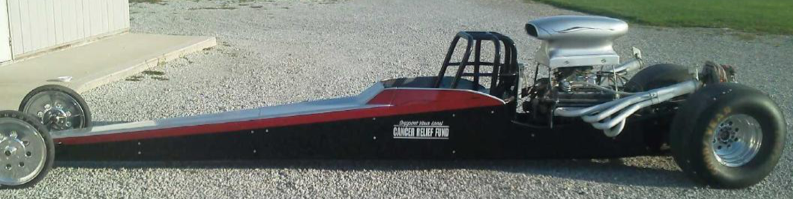
\includegraphics{images/drag.png}
Very aerodynamic and fast, but not comfortable for the long run (more than about 8 seconds).
You will need something more like a production car, with a nice interior and a dashboard, and comfy leather seats.
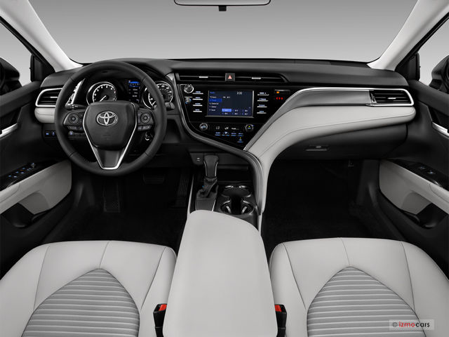
\includegraphics{images/dashboard.png}
This is provided by the RStudio IDE (Integrated Developer Environment). We want you to install both R and RStudio, in that order.\\
Let's start with installing R.\\
R is free and available for download on the web. Go to the \href{https://r-project.org/}{r-project website} to get started.

This screen will look like this
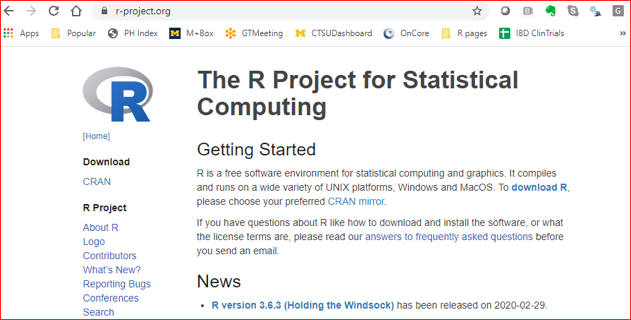
\includegraphics{images/r-project.png}\\
You can see from the blue link (download R) that you can download R, but you will be downloading it faster if you pick a local CRAN mirror.\\
You might be wondering what CRAN and CRAN Mirrors are. Nothing to do with cranberries, fortunately. CRAN is the Comprehensive R Archive Network. Each site (mirror) in the network contains an archive of all R versions and packages, and the sites are scattered over the globe. A CRAN Mirror maintains an up to date copy of all of the R versions and packages on CRAN. If you use the nearest CRAN mirror, you will generally get faster downloads.\\
At this point, you might be wondering what a package is\ldots{}\\
A package is a set of functions and/or data that you can download to upgrade and add features to R. It is a lot like a downloadable upgrade to a Tesla that lets you play the video game \emph{Witcher 3} on your console, but more useful.
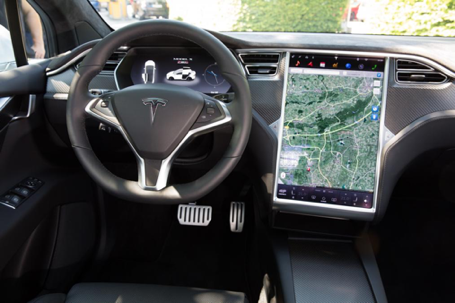
\includegraphics{images/dash-tesla.png}

Now click on the blue link that says ``download R''.\\
This will take you to a page to select your local CRAN Mirror , from which you will download R.
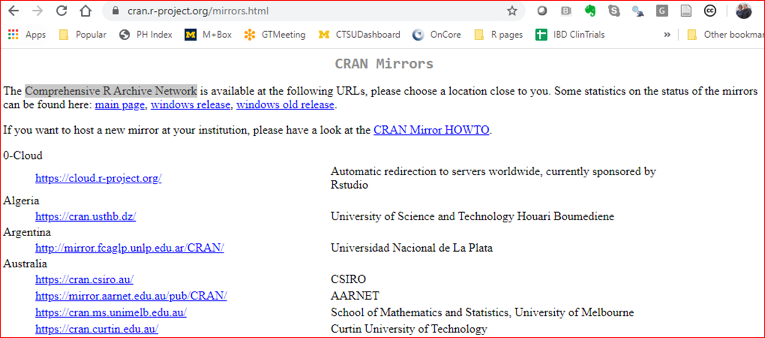
\includegraphics{images/cran-mirror.png}
Scroll down to your country (yes, the USA is at the bottom), and a CRAN mirror near you.
This is an example from northern Michigan, USA.
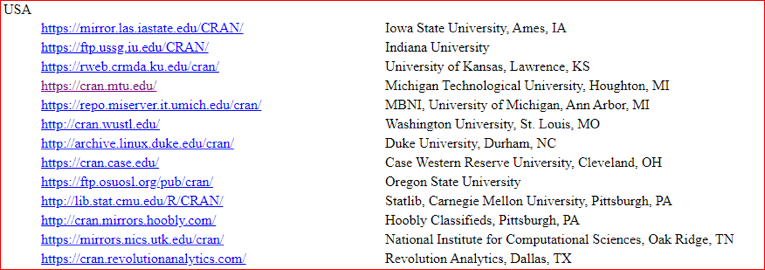
\includegraphics{images/usa-mirrors.png}
Once you click on a CRAN Mirror site to select the location, you will be taken to the actual Download site.

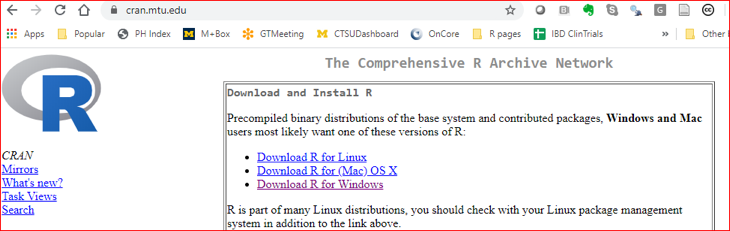
\includegraphics{images/installr.png}
Select the link for the operating system you want to use. We will walk through this with Windows first, then Mac. If you are using a Mac, skip forward to the Mac install. If you are using Linux, you can clearly figure it out on your own (it will look a lot like these).\\
Once you have clicked through, your next screen will look like this\\
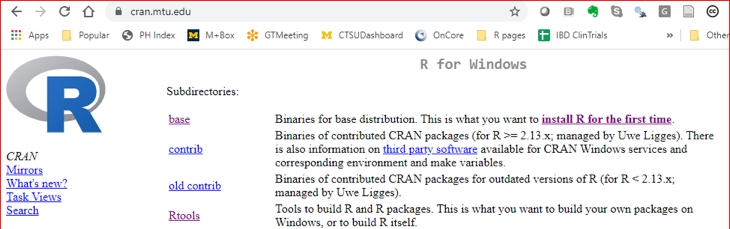
\includegraphics{images/installr2.png}
You want to download both base and Rtools (you might need Rtools later). The base link will take you to the latest version, which will look something like this.

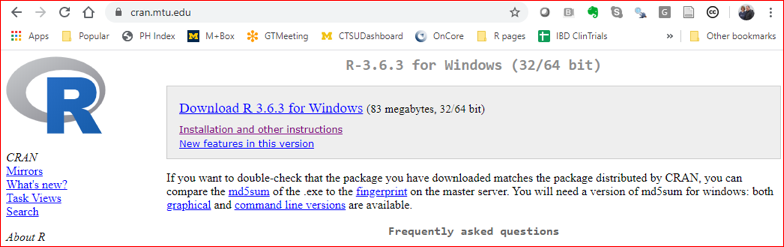
\includegraphics{images/installr3windows.png}
Click on this link, and you will be able to save a file named R-N.N.N-win.exe (Ns depending on version number) to your Downloads folder. Click on the Save button to save it.
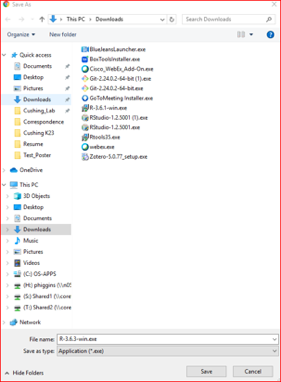
\includegraphics{images/installrsave.png}
Now, go to your Downloads folder in Windows, and double clinic on the R installation file (R-N.N.N-win.exe). Click Yes to allow this to install.
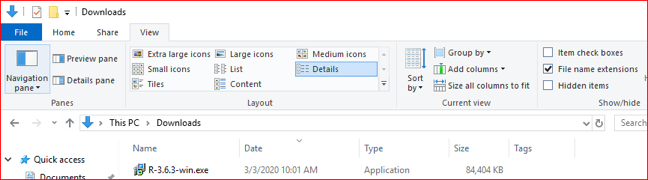
\includegraphics{images/installrexe.png}
Now select your language option
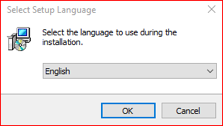
\includegraphics{images/installrEnglish.png}
You will be asked to accept the GNU license - do so. Click Yes to allow this to install. Then select where to install - generally use the default- a local (often C) drive - do not install on a shared network drive or in the cloud.
\includegraphics{images/installrdrive.png}
Then select the Components - generally use the defaults, but newer computers can skip the 32 bit version.
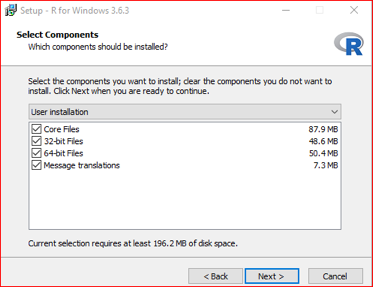
\includegraphics{images/installrComponents.png}
In the next dialog box, accept the default startup options.
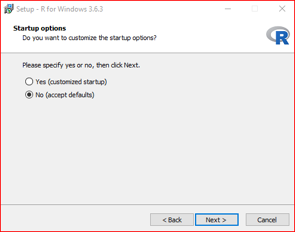
\includegraphics{images/installrdefaults.png}
You can choose the start menu folder. The default R folder is fine.
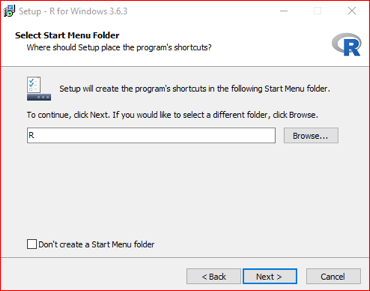
\includegraphics{images/installrstartmenu.png}

You probably won't need shortcuts, so leave these unchecked in the next dialog box.
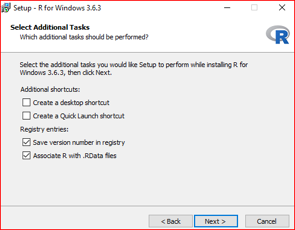
\includegraphics{images/installraddltasks.png}

Then the Setup Wizard will appear - click Finish, and the rest of the installation will occur.

\begin{figure}
\centering
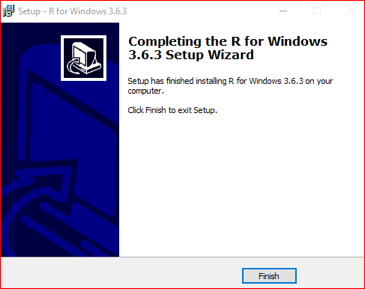
\includegraphics{images/installrwizard.png}
\caption{install\_wizard}
\end{figure}

\hypertarget{testing}{%
\subsection{Testing}\label{testing}}

Now you want to test whether your Windows installation was successful. Can you find R and make it work?
Hunt for your C folder, then for OS-APPS within that folder. Keep drilling down to the Program Files folder. Then the R folder, and the current version folder within that one (R-N.N.N). Within that folder will be the bin folder, and within that will be your R-N.N.N.exe file. Double click on this to run it. The example paths below can help guide you.

\begin{figure}
\centering
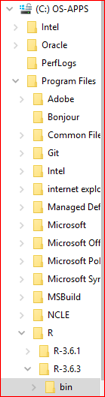
\includegraphics{images/installwin-path2.png}
\caption{install\_path2}
\end{figure}

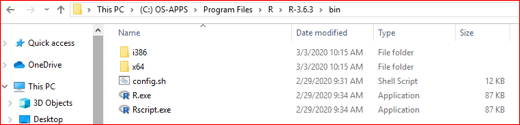
\includegraphics{images/installrpath.png}
Opening the exe file will produce a classic 2000-era terminal window, called Rterm, with 64 bit if that is what your computer uses. The version number should match what you downloaded. The messaging should end with a ``\textgreater{}'' prompt.
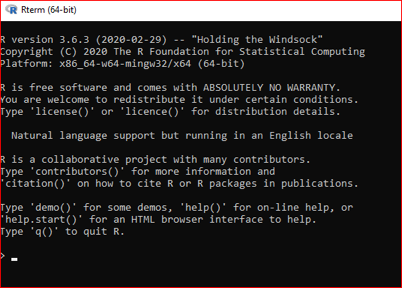
\includegraphics{images/windowsrterm.png}
At this prompt, type in:\\
paste(`Two to the seventh power is', 2\^{}7)
(don't leave out the comma) - then press the Enter key.

This should produce the following:

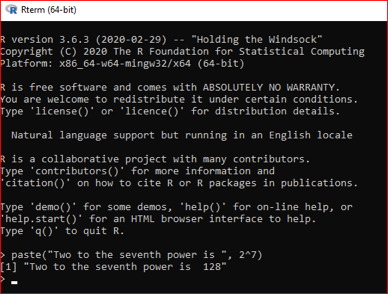
\includegraphics{images/windowstest.png}
Note that you have explained what is being done and computed the result.

\hypertarget{mac-install-of-r}{%
\subsection{Mac Install of R}\label{mac-install-of-r}}

The installation for Mac is very similar, but the windows look a bit different. At the Download Version page, you click on the Mac Download.
You will then click on the link for R-N.N.N.pkg, and allow downloads from CRAN.

\begin{figure}
\centering
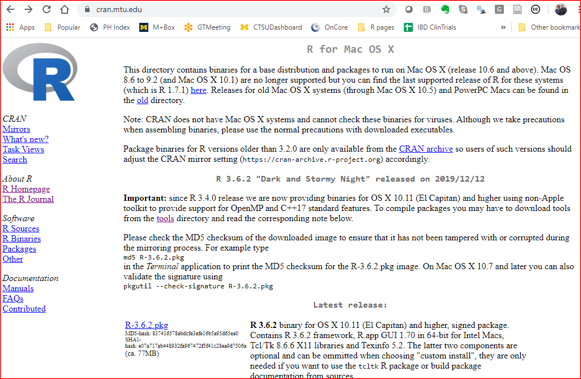
\includegraphics{images/installrpkgmac.png}
\caption{install\_path}
\end{figure}

Then go to Finder, and navigate to the Downloads folder. Click on R-N.N.N.pkg
You will then click on the link for R-N.N.N.pkg, and allow downloads from CRAN.

\includegraphics{images/installrdownloadsmac.png}
Click on Continue on 2 consecutive screens to download


\includegraphics{images/installrCont1mac.png}
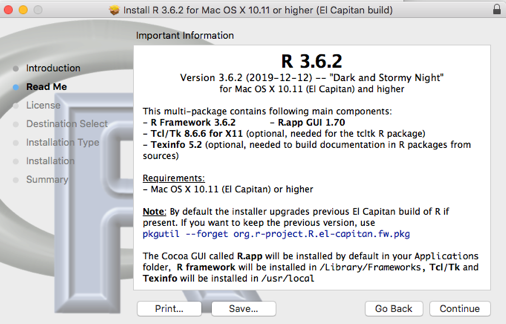
\includegraphics{images/installrCont2mac.png}
Then you need to agree with the License Agreement,
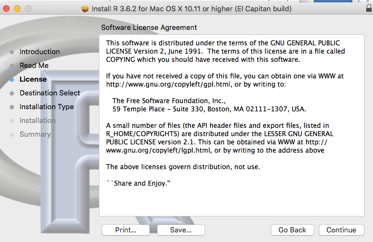
\includegraphics{images/installrmacLicense.png}
then Click on Install, and provide your Mac password for permission to install.
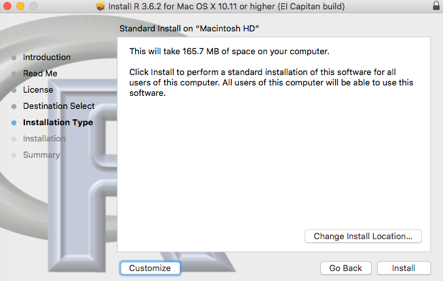
\includegraphics{images/installrmac-install.png}
When the installation is complete, click on the Close button. Accept the prompt to move the installer file to the trash.

\hypertarget{testing-r-on-the-mac}{%
\subsection{Testing R on the Mac}\label{testing-r-on-the-mac}}

Go to Finder, and then your Applications folder. Scroll down to the R file. Double click on this to run it.
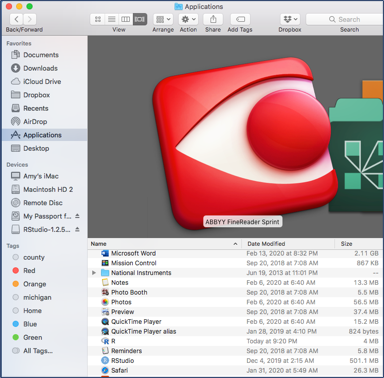
\includegraphics{images/findrmac.png}
You should get this 2000=era terminal window named R Console. The version number should match what you downloaded, and the messaging should end with a ``\textgreater{}'' prompt.
At this prompt, type in
paste(`Two to the seventh power is', 2\^{}7)
(DON'T leave out the comma)
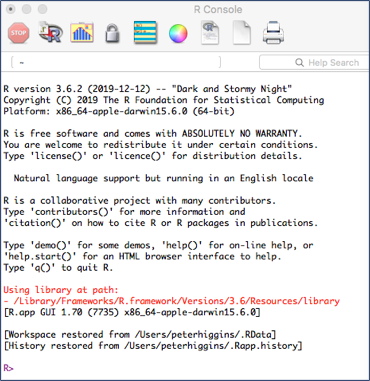
\includegraphics{images/rconsolemac.png}

This should result in

\begin{figure}
\centering
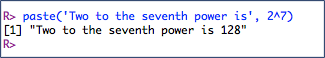
\includegraphics{images/mactestR.png}
\caption{mactestR}
\end{figure}

\hypertarget{successful-testing}{%
\subsection{Successful testing!}\label{successful-testing}}

Awesome. You are now Ready to R!
\includegraphics{images/ready2R.png}

\hypertarget{installing-rstudio-on-your-computer}{%
\section{Installing RStudio on your Computer}\label{installing-rstudio-on-your-computer}}

\hypertarget{installing-git-on-your-computer}{%
\section{Installing Git on your Computer}\label{installing-git-on-your-computer}}

\hypertarget{getting-acquainted-with-the-rstudio-ide}{%
\section{Getting Acquainted with the RStudio IDE}\label{getting-acquainted-with-the-rstudio-ide}}

\hypertarget{intro}{%
\section{Introduction}\label{intro}}

There are many books about Data Science.
Why does the world need another one, particularly one targeting physicians?

\begin{itemize}
\tightlist
\item
  There is a lot of health care data
\item
  There are a lot of interesting questions in health care
\item
  There are particular and challenging issues in doing data analysis with PHI (Protected Health Information)
\end{itemize}

Syllabus: Data Science for Physicians (DS4P)

\begin{itemize}
\tightlist
\item
  Instructor: Peter Higgins, MD, PhD, MSc (CRDSA), Professor of Internal Medicine
\item
  Office Hours: MSRB One 6510
\item
  In-person class time

  \begin{itemize}
  \tightlist
  \item
    MSRB One 6510, Thursday evenings 6:30-8:30 PM
  \end{itemize}
\end{itemize}

\hypertarget{course-description-and-objectives}{%
\section{Course Description and Objectives}\label{course-description-and-objectives}}

\hypertarget{description}{%
\subsection{Description}\label{description}}

A practical introduction to data collection and security, data cleaning, statistical methods and computational tools needed to make sense of data, and methods for reporting and sharing your findings. This course is not a traditional introductory statistics courses in that computing plays a more central role than mathematics and a higher emphasis is placed on ``thinking with data.'' Topics include

\begin{itemize}
\tightlist
\item
  secure HIPPA-compliant data collection
\item
  data cleaning and validation
\item
  data visualization
\item
  data wrangling
\item
  confidence intervals
\item
  hypothesis testing, and
\item
  regression
  The course has no mathematics or computer science prerequisites.
\end{itemize}

\hypertarget{objectives}{%
\subsection{Objectives}\label{objectives}}

\begin{enumerate}
\def\labelenumi{\arabic{enumi}.}
\tightlist
\item
  Have students engage in the data/science research pipeline in as faithful a manner as possible while maintaining a level suitable for novices.
\item
  Foster a conceptual understanding of statistical topics and methods using real clinical data whenever possible, and simulation/resampling to support teaching concepts of inference.
\item
  Use a flipped classroom model by incorporating online learning for new concepts, with limited face-to-face time for real-time problem-solving
\item
  Introduce best practices for reproducible research and collaboration.
\item
  Develop statistical literacy by, among other ways, tying in the curriculum to actual clinical data, demonstrating the importance statistics and computing plays in advancing medicine
\end{enumerate}

\hypertarget{topics}{%
\subsection{Topics}\label{topics}}

Roughly speaking we will cover the following topics (a more detailed outline is found below:

\begin{enumerate}
\def\labelenumi{\arabic{enumi}.}
\tightlist
\item
  Introduction and Tools (R, RStudio, and R Markdown)
\item
  Data Import, and Handling
\item
  Data Collection
\item
  Checking, Validating, And Exploring your Data
\item
  Data Types
\item
  Data Wrangling with Tidyr and Dplyr
\item
  Graphic Summaries for a Single Variable -- ggplot package
\item
  Descriptive Data for a Single Variable
\item
  Graphic Summaries for Two or More Variables -- ggplot2
\item
  Descriptive Data for Two or More Variables
\item
  Presenting your Results in a report with RMarkdown
\item
  Statistical inference
\item
  Study Design
\item
  Sample Size and Power
\item
  Sources of Bias
\item
  Study Types
\item
  One variable, single group
\item
  One variable, two groups
\item
  Multiple groups
\item
  Linear Regression
\item
  Reporting results interactively with Shiny
\item
  Logistic Regression
\item
  Meta-Analysis
\end{enumerate}

\hypertarget{learning-resources}{%
\subsection{Learning Resources}\label{learning-resources}}

• E-Textbooks:
Open Intro Statistics, at www.openintro.org

• E-Books on R
These are at different levels:

Level: Absolute Beginner
Textbook: R Basics\\
Goal: Set up R and RStudio on a laptop, introduce the concept of an IDE\\
Link:

Level: New to R \& Statistics\\
Textbook: Modern Dive
Goal: Learn basics of Data Management and visualization, introduction to hypothesis testing and statistical modeling\\
Link:

Level: Comfortable with R\\
Textbook: Hands-On R Programming\\
Goal:\\
Link:

Level: Ready to Understand More\\
Textbook: R for Data Science\\
Link:\\

• Software:

\begin{itemize}
\tightlist
\item
  Local laptop/desktop free open-source version of R and RStudio
\item
  Cloud-based RStudio Server, which you can access in your browser via:
  Note if you are off-campus you must first log into the UM VPN.
\end{itemize}

• Online:

\begin{itemize}
\tightlist
\item
  DataCamp. A brower based interactive tool for learning R through short, focused courses, each 3-4 hours long.
\item
  RStudio. Website with many resources for learning about the RStudio IDE and the tidyverse.
\item
  r-cookbook -- an often useful website with concrete examples of how to use R packages
\item
  Stack Overflow and Google. Remarkably helpful to search for explanations of error messages, or explanations of problems that someone else has probably also experienced. For using Google, search for any topic or your error message and add ``in R''
\item
  package vignettes -- variable quality, but when well done, can be extremely helpful examples of how to use the functions in each package
\item
  R twitter -- follow Rbloggers, \#rstats
\end{itemize}

\hypertarget{evaluation}{%
\subsection{Evaluation}\label{evaluation}}

This course is entirely voluntary. I hope that you will learn valuable skills that will advance your research career. I would like you to progress to using these skills on your own data as quickly as possible, as this will greatly help you reinforce your new skills. There are no grades and no formal evaluations. You can, however, earn certificates on DataCamp for completing courses.

\hypertarget{task-goals}{%
\subsection{Task Goals}\label{task-goals}}

\begin{enumerate}
\def\labelenumi{\arabic{enumi}.}
\tightlist
\item
  Learn concepts through Data Camp\\
\end{enumerate}

\begin{enumerate}
\def\labelenumi{\alph{enumi}.}
\tightlist
\item
  Multiple short courses to correspond with each unit
\end{enumerate}

\begin{enumerate}
\def\labelenumi{\arabic{enumi}.}
\setcounter{enumi}{1}
\tightlist
\item
  Test yourself with assignments in ModernDive
\end{enumerate}

\begin{enumerate}
\def\labelenumi{\alph{enumi}.}
\tightlist
\item
  Chapters corresponding to each unit
\end{enumerate}

\begin{enumerate}
\def\labelenumi{\arabic{enumi}.}
\setcounter{enumi}{2}
\tightlist
\item
  Three Challenges
\end{enumerate}

\begin{enumerate}
\def\labelenumi{\alph{enumi}.}
\tightlist
\item
  Clean data and perform descriptive data analysis on the biofire dataset
\item
  Clean data and model outcomes in the health satisfaction dataset, producing a final report
\item
  Use logistic regression to model dichotomous outcomes and produce a Shiny app to allow users to make predictions for future patients
\end{enumerate}

\begin{enumerate}
\def\labelenumi{\arabic{enumi}.}
\setcounter{enumi}{3}
\tightlist
\item
  Final Project
  There will be a final capstone project. This is an opportunity for you to use your statistics and data science skills developed during the challenges and perform your own start-to-finish data analysis project. The project will involving you addressing a scientific question by choosing a data set (or preferably, using one of your own), performing an analysis using the concepts and tools we have covered in this course, and writing a report. This can be done solo or with a partner.
\end{enumerate}

\hypertarget{learning-goals}{%
\subsection{Learning Goals}\label{learning-goals}}

\begin{enumerate}
\def\labelenumi{\arabic{enumi}.}
\tightlist
\item
  Recognize the importance of data collection, identify limitations in data collection methods, and determine how they affect the generalizability of your findings
\item
  Use statistical software (R) to summarize data numerically and visually, and to perform data analysis.
\item
  Have a conceptual understanding of statistical inference.
\item
  Apply estimation and testing methods to analyze single variables or the relationship between two variables in order to understand data relationships and make data-based conclusions.
\item
  Model numerical response variables and dichotomous response variables using a single explanatory variable or multiple explanatory variables in order to investigate relationships between variables.
\item
  Interpret results correctly, effectively, and in context without relying on statistical jargon.
\item
  Critique data-based claims and evaluate data-based decisions.
\end{enumerate}

\hypertarget{tips-for-success}{%
\subsection{Tips for success}\label{tips-for-success}}

\begin{enumerate}
\def\labelenumi{\arabic{enumi}.}
\tightlist
\item
  Read materials for each unit
\item
  Do Data Camp courses for each unit -- usually around 1 chapter (1 hour) per day.
\item
  Do Data Camp daily practice on any day that you don't have time to do a full chapter
\item
  At end of each course, review material, take notes, copy/reproduce/save code on your laptop
\item
  Try new skills on your own data, or on one of the open data sets
\item
  Use RStudio and DataCamp Cheat sheets
\item
  Annotate your code to help `future you' understand it.
\item
  Save and reuse your code for future projects
\end{enumerate}

\hypertarget{expected-work-load}{%
\subsection{Expected work load}\label{expected-work-load}}

This course is entirely voluntary. It is expected that you have lots of clinical and/or research work to keep up with, along with the occasional call or night rotation. This is an investment in future skills to help your career. I recommend that you try to do up to one hour a day on most days, and on days when that is not realistic, to just do the 10 minutes of daily practice on DataCamp to keep the information fresh in your mind.\\
Other learning resources:

You can label chapter and section titles using \texttt{\{\#label\}} after them, e.g., we can reference Chapter \ref{intro}. If you do not manually label them, there will be automatic labels anyway, e.g., Chapter \ref{methods}.

Figures and tables with captions will be placed in \texttt{figure} and \texttt{table} environments, respectively.

\begin{Shaded}
\begin{Highlighting}[]
\KeywordTok{par}\NormalTok{(}\DataTypeTok{mar =} \KeywordTok{c}\NormalTok{(}\DecValTok{4}\NormalTok{, }\DecValTok{4}\NormalTok{, }\FloatTok{.1}\NormalTok{, }\FloatTok{.1}\NormalTok{))}
\KeywordTok{plot}\NormalTok{(pressure, }\DataTypeTok{type =} \StringTok{'b'}\NormalTok{, }\DataTypeTok{pch =} \DecValTok{19}\NormalTok{)}
\end{Highlighting}
\end{Shaded}

\begin{figure}

{\centering 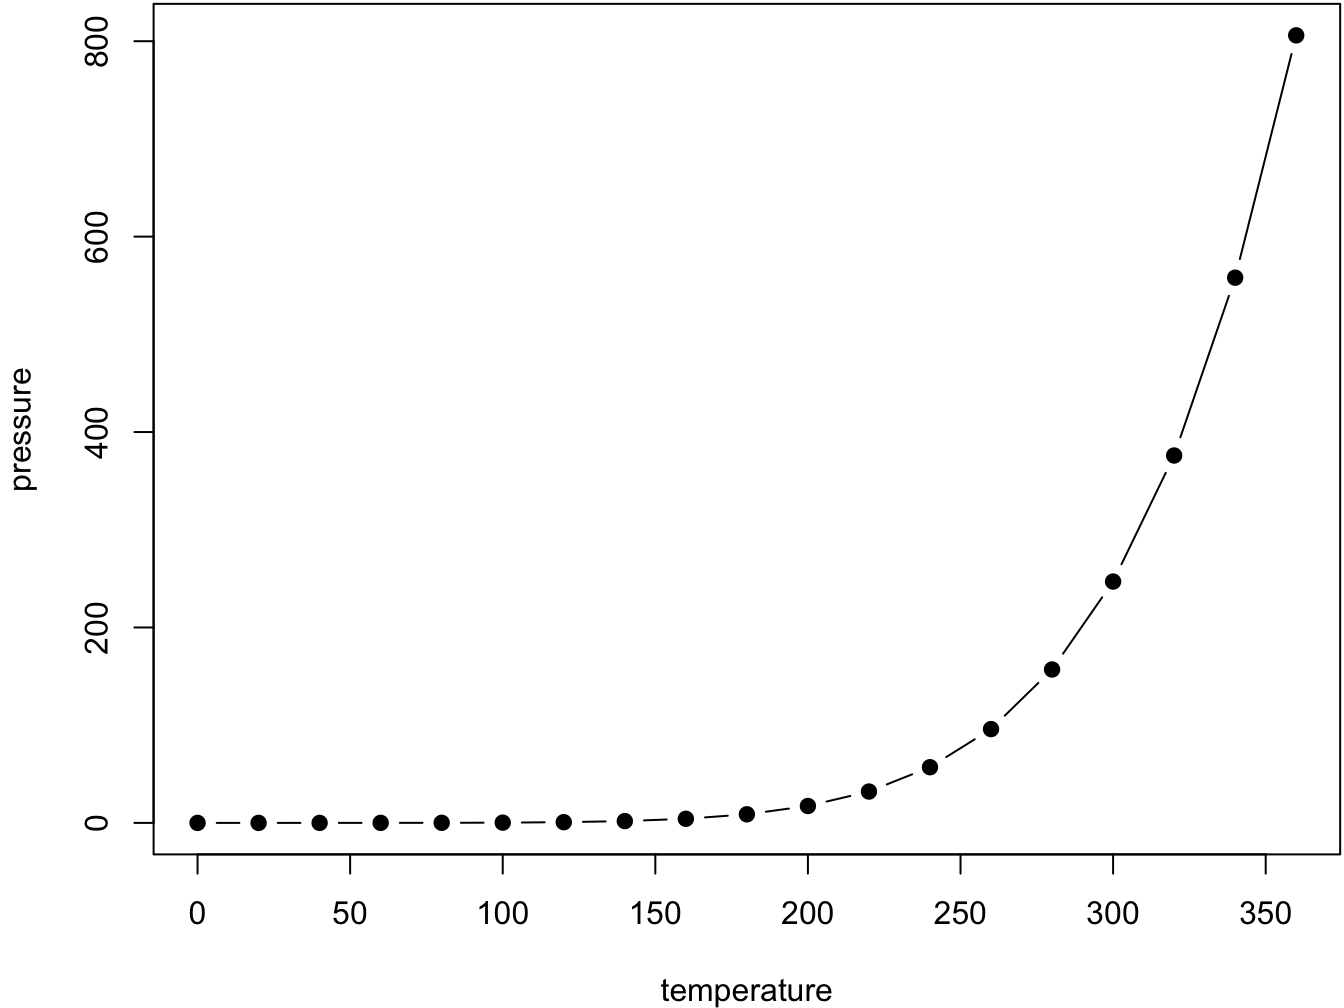
\includegraphics[width=0.8\linewidth]{io02-getting-started_files/figure-latex/nice-fig-1} 

}

\caption{Here is a nice figure!}\label{fig:nice-fig}
\end{figure}

Reference a figure by its code chunk label with the \texttt{fig:} prefix, e.g., see Figure \ref{fig:nice-fig}. Similarly, you can reference tables generated from \texttt{knitr::kable()}, e.g., see Table \ref{tab:nice-tab}.

\begin{Shaded}
\begin{Highlighting}[]
\NormalTok{knitr}\OperatorTok{::}\KeywordTok{kable}\NormalTok{(}
  \KeywordTok{head}\NormalTok{(iris, }\DecValTok{20}\NormalTok{), }\DataTypeTok{caption =} \StringTok{'Here is a nice table!'}\NormalTok{,}
  \DataTypeTok{booktabs =} \OtherTok{TRUE}
\NormalTok{)}
\end{Highlighting}
\end{Shaded}

\begin{table}

\caption{\label{tab:nice-tab}Here is a nice table!}
\centering
\begin{tabular}[t]{rrrrl}
\toprule
Sepal.Length & Sepal.Width & Petal.Length & Petal.Width & Species\\
\midrule
5.1 & 3.5 & 1.4 & 0.2 & setosa\\
4.9 & 3.0 & 1.4 & 0.2 & setosa\\
4.7 & 3.2 & 1.3 & 0.2 & setosa\\
4.6 & 3.1 & 1.5 & 0.2 & setosa\\
5.0 & 3.6 & 1.4 & 0.2 & setosa\\
\addlinespace
5.4 & 3.9 & 1.7 & 0.4 & setosa\\
4.6 & 3.4 & 1.4 & 0.3 & setosa\\
5.0 & 3.4 & 1.5 & 0.2 & setosa\\
4.4 & 2.9 & 1.4 & 0.2 & setosa\\
4.9 & 3.1 & 1.5 & 0.1 & setosa\\
\addlinespace
5.4 & 3.7 & 1.5 & 0.2 & setosa\\
4.8 & 3.4 & 1.6 & 0.2 & setosa\\
4.8 & 3.0 & 1.4 & 0.1 & setosa\\
4.3 & 3.0 & 1.1 & 0.1 & setosa\\
5.8 & 4.0 & 1.2 & 0.2 & setosa\\
\addlinespace
5.7 & 4.4 & 1.5 & 0.4 & setosa\\
5.4 & 3.9 & 1.3 & 0.4 & setosa\\
5.1 & 3.5 & 1.4 & 0.3 & setosa\\
5.7 & 3.8 & 1.7 & 0.3 & setosa\\
5.1 & 3.8 & 1.5 & 0.3 & setosa\\
\bottomrule
\end{tabular}
\end{table}

You can write citations, too. For example, we are using the \textbf{bookdown} package \citep{R-bookdown} in this sample book, which was built on top of R Markdown and \textbf{knitr} \citep{xie2015}.

\hypertarget{access-rstudio-cloud}{%
\section{Access RStudio cloud}\label{access-rstudio-cloud}}

\hypertarget{r-basics-e-book}{%
\section{R basics E-book}\label{r-basics-e-book}}

Use the e-book Rbasics by Chester Ismay

\url{https://ismayc.github.io/rbasics-book/}

\hypertarget{rstudio-tips-document}{%
\section{RStudio tips document}\label{rstudio-tips-document}}

\hypertarget{a-tasting-menu-of-r}{%
\chapter{A Tasting Menu of R}\label{a-tasting-menu-of-r}}

In this chapter, we will introduce you to a lot of neat things that you can do with R and RStudio, and you will publish a simple data analysis on the Internet
that you can share with friends and family.
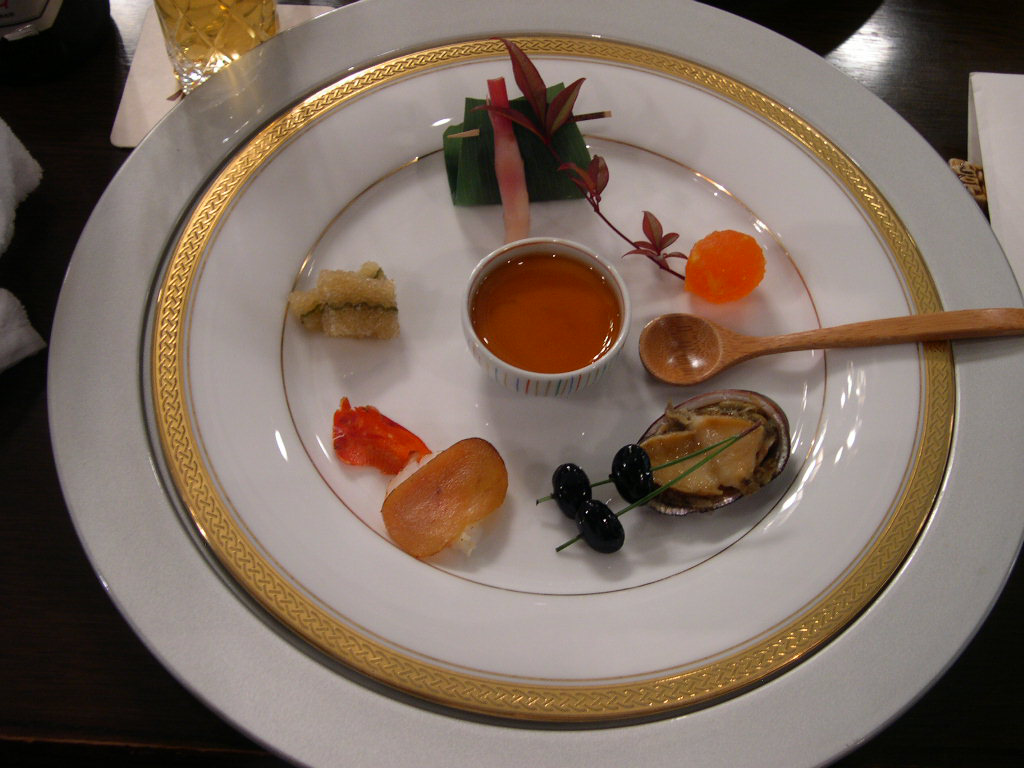
\includegraphics{images/tasting.png}

\hypertarget{setting-the-table}{%
\section{Setting the Table}\label{setting-the-table}}

At the end of this chapter, you will publish a data analysis to \emph{RPubs}, a free website site where you can share your data analyses and visualizations. First you will need to set up an account on RPubs. Start by opening a new tab in your browser, and navigating to this \href{https://rpubs.com/users/new}{RPubs link}. It should look like the image below.
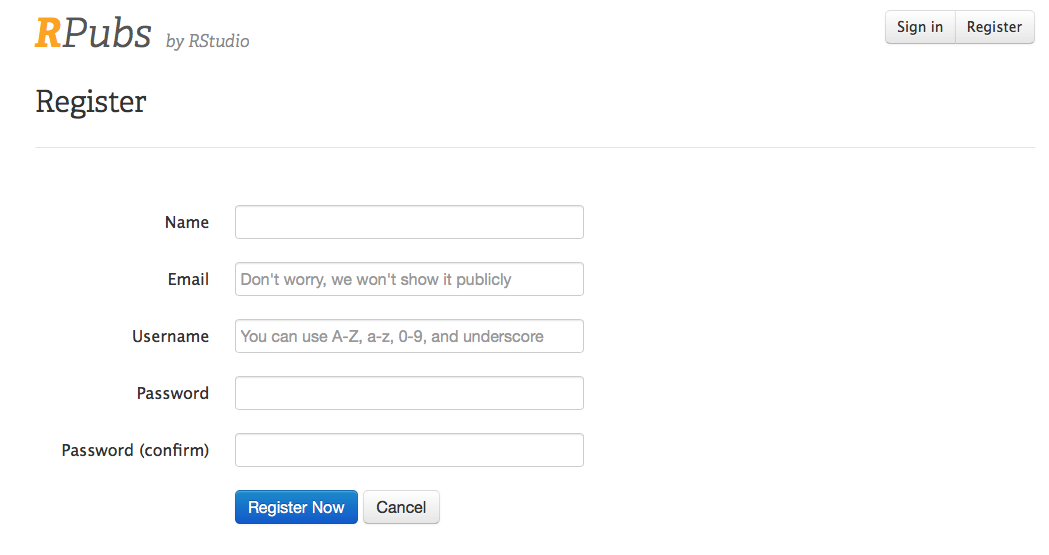
\includegraphics{images/rpubs1.png}\\
Enter your name, email, username and password, and click on the \emph{Register Now} button, and you will be set up to use RPubs.\\
This will bring you to this page. In the image below, we have set up an account for pdr.\\
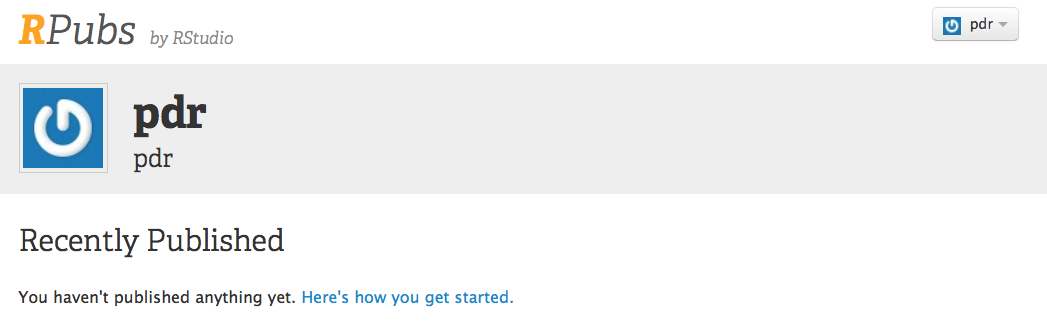
\includegraphics{images/rpubs2.png}
Click on the \emph{Here's How You Get Started} link.
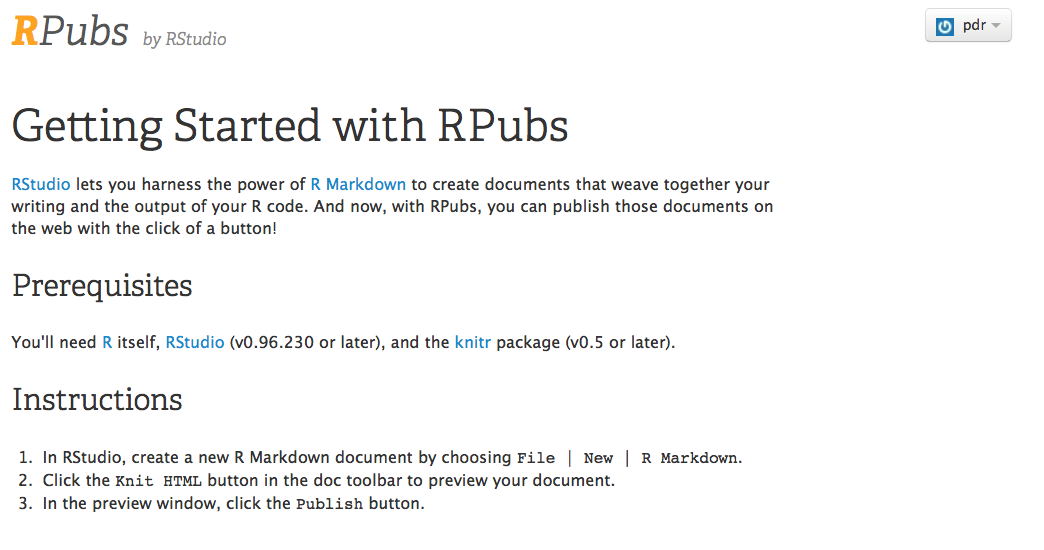
\includegraphics{images/rpubs3.png}\\
You are now all set up and ready to go. Now you have a place on the internet to share your R creations!

\hypertarget{goals-for-this-chapter-1}{%
\section{Goals for this Chapter}\label{goals-for-this-chapter-1}}

\begin{itemize}
\tightlist
\item
  Open a New Rmarkdown document
\item
  Read in Data from a file
\item
  Wrangle Your Data
\item
  Visualize Your Data
\item
  Publish your work to RPubs
\item
  Check out Interactive Plots
\item
  Check out Animated Graphics
\item
  Check out a Clinical Trial Dashboard
\item
  Check out a Shiny App
\end{itemize}

\hypertarget{packages-needed-for-this-chapter}{%
\section{Packages needed for this Chapter}\label{packages-needed-for-this-chapter}}

You will need to enter this line of code into your console, to make sure that the tidyverse package is installed on your computer.
\texttt{install.packages("tidyverse")}

In the setup chunk of your Rmarkdown document, you will need to access the tidyverse package with one line of code:
\texttt{library(tidyverse)}

\hypertarget{website-links-needed-for-this-chapter-1}{%
\section{Website links needed for this Chapter}\label{website-links-needed-for-this-chapter-1}}

In this chapter, you will need to access the RPubs website.\\
- \url{https://rpubs.com/}

\hypertarget{pathway-for-this-chapter-1}{%
\section{Pathway for this Chapter}\label{pathway-for-this-chapter-1}}

This Chapter is part of the \textbf{XXX} pathway.
Chapters in this pathway include

\hypertarget{open-a-new-rmarkdown-document}{%
\section{Open a New Rmarkdown document}\label{open-a-new-rmarkdown-document}}

Let's get started in R. Turn on your computer, and open the RStudio application. You should see the familiar panes for the Console, Environment, and Files.\\
You need to open up a new document to activate the Source pane. While in RStudio, click on File/New File/R Script.
It should look like this.\\
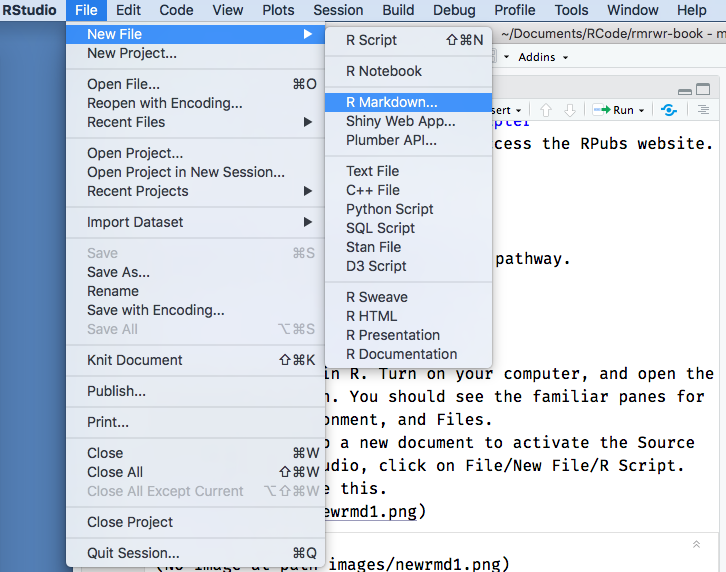
\includegraphics{images/rmd1.png}
Now you will see the window below. Rename the document from ``Untitled'' to ``Tasting'', and click the OK button.
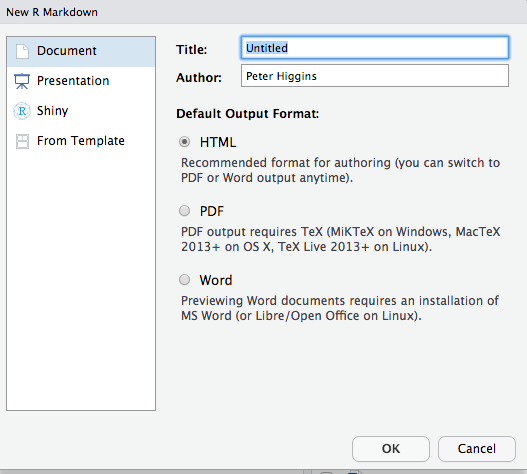
\includegraphics{images/rmd2.png}

Now the file is open, and looks like the window below. Click on the save icon (like a floppy disk in the top left), and save this document as tasting.Rmd.
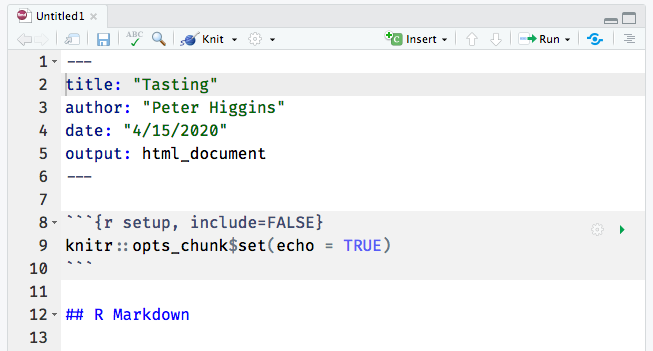
\includegraphics{images/rmd3.png}
You have created a new Rmarkdown document. An Rmarkdown document lets you mix data, code, and descriptive text. It is very helpful for presenting and explaining data and visualizations. An Rmarkdown document can be converted (Knit) to HTML for a web page, Microsoft Word, Powerpoint, PDF, and several other formats.

Code chunks are in a gray color, and both start and end with 3 backticks (```).

Text can be body text, or can be headers and titles. The number of hashtags before some header text defines what level the header is.\\
You can insert links, pictures, and YouTube videos into Rmarkdown documents if it is helpful to explain your point.
The first code chunk in each Rmarkdown document is named \texttt{setup}. The name comes after the left curly brace and the r (\texttt{\{r}) at the beginning of the setup chunk. The letter \texttt{r} tells RStudio that what is coming on the next line is R code (RStudio can also use SQL, C++, python, and several other languages). After the comma, you can define options for this code chunk. In this case, the option \texttt{include} is set to FALSE, so that when this Rmarkdown document is knitted, this code chunk will not appear.

\hypertarget{read-in-data-from-a-file}{%
\section{Read in Data from a file}\label{read-in-data-from-a-file}}

\hypertarget{wrangle-your-data}{%
\section{Wrangle Your Data}\label{wrangle-your-data}}

\hypertarget{visualize-your-data}{%
\section{Visualize Your Data}\label{visualize-your-data}}

\hypertarget{publish-your-work-to-rpubs}{%
\section{Publish your work to RPubs}\label{publish-your-work-to-rpubs}}

\hypertarget{the-dessert-cart}{%
\section{The Dessert Cart}\label{the-dessert-cart}}

Below are some examples of neat things you can do with medical data in R. These are more advanced approaches, but completely doable when you have more experience with R.

\hypertarget{interactive-plots}{%
\subsection{Interactive Plots}\label{interactive-plots}}

\hypertarget{animated-graphics}{%
\subsection{Animated Graphics}\label{animated-graphics}}

\hypertarget{a-clinical-trial-dashboard}{%
\subsection{A Clinical Trial Dashboard}\label{a-clinical-trial-dashboard}}

\hypertarget{a-shiny-app}{%
\subsection{A Shiny App}\label{a-shiny-app}}

\hypertarget{an-example-of-synergy-in-the-r-community}{%
\subsection{An Example of Synergy in the R Community}\label{an-example-of-synergy-in-the-r-community}}

One of the remarkable things about the open source R community is that people build all kinds of new R functions and packages that are useful to them, and then share them publicly with tools like \emph{Github} so that they can be useful to others. Often combining bits of several packages leads to \textbf{emergent properties} - completely new creations that can only occur because all of the parts (packages) are present. The collaborative nature of the R community, in this case on Twitter (follow the \#rstats hashtag), can lead to surprising collaborations and outcomes.\\
See the example below.\\
Go ahead, \emph{click} on the play button to run the gifs. All coded in R.\\

I used a modified version of \citet{djnavarro}'s flametree package to produce this fractal tree in 3D, placed it in a LEGO planter for \citet{ryantimpe}, set down a copy of \citet{skyetetra} and \citet{robinson_es}'s book for some light reading, and of course, used \#rayrender and \#rstats to render it all :) https://t.co/qRg2omUftw pic.twitter.com/Ff9VeLtX97

--- Tyler Morgan-Wall (\citet{tylermorganwall}) April 14, 2020

\hypertarget{updating-r-rstudio-and-your-packages}{%
\chapter{Updating R, RStudio, and Your Packages}\label{updating-r-rstudio-and-your-packages}}

This is an R Markdown document. Markdown is a simple formatting syntax for authoring HTML, PDF, and MS Word documents. For more details on using R Markdown see \url{http://rmarkdown.rstudio.com}.

\hypertarget{major-r-updates-where-are-my-packages}{%
\chapter{Major R Updates (Where Are My Packages?)}\label{major-r-updates-where-are-my-packages}}

This is an R Markdown document. Markdown is a simple formatting syntax for authoring HTML, PDF, and MS Word documents. For more details on using R Markdown see \url{http://rmarkdown.rstudio.com}.

\hypertarget{checking-validating-and-asserting-things-about-your-data}{%
\chapter{Checking, Validating, And Asserting things about your Data}\label{checking-validating-and-asserting-things-about-your-data}}

So you have imported your data!
Great!
Now to start the analysis!

Not so fast, cowboy!\\
First you need to validate your data.

\hypertarget{cleaning-names-with-janitor-package-to-snake_case}{%
\subsubsection{Cleaning -- names with janitor package to snake\_case}\label{cleaning-names-with-janitor-package-to-snake_case}}

\hypertarget{a-few-words-about-tidyverse-style}{%
\paragraph{A few words about tidyverse style}\label{a-few-words-about-tidyverse-style}}

\hypertarget{finding-missing-data-naniar-and-visdat-packages}{%
\subsubsection{Finding Missing data -- naniar and visdat packages}\label{finding-missing-data-naniar-and-visdat-packages}}

\hypertarget{validating-data-validate-package}{%
\subsubsection{Validating data -- validate package}\label{validating-data-validate-package}}

\hypertarget{asserting-properties-of-your-data-with-assertr}{%
\subsection{Asserting properties of your data with assertr}\label{asserting-properties-of-your-data-with-assertr}}

\hypertarget{evaluating-str-glimpse}{%
\subsubsection{Evaluating -- str, glimpse}\label{evaluating-str-glimpse}}

\hypertarget{exploring--skimr-package}{%
\subsubsection{Exploring- skimr package}\label{exploring--skimr-package}}

\hypertarget{histograms}{%
\subsubsection{Histograms}\label{histograms}}

\hypertarget{correlations-ggally-extension-of-ggplot2-and-corrr-package}{%
\subsubsection{Correlations -- ggally extension of ggplot2, and corrr package}\label{correlations-ggally-extension-of-ggplot2-and-corrr-package}}

\hypertarget{time-series-data-with-the-tidyverts-packages}{%
\chapter{Time Series data with the Tidyverts Packages}\label{time-series-data-with-the-tidyverts-packages}}

Fun text here.
All kinds of crazy examples.
Time series with data from influenza pandemic of 1918-19, perhaps.
This is a book for anyone in the medical field interested in analyzing the data available to them to better understand health, disease, or delivery of care. This could include nurses, dieticians, psychologists, and PhDs in related fields, as well as medical students, residents, fellows, or doctors in practice.\\
I expect that most learners will be using this book in their spare time at night and on weekends, as the medical school curriculum is already packed full, and there is no room to add skills in reproducible research to the standard curriculum. This book is designed for self-teaching, and many hints and solutions will be provided to avoid roadblocks and frustration.

\hypertarget{tsibble}{%
\section{Tsibble}\label{tsibble}}

Time series tibble

\href{https://tidyverts.org}{Tidyverts webpage}

\hypertarget{fable}{%
\section{Fable}\label{fable}}

Tidy forecasting

\hypertarget{feasts}{%
\section{Feasts}\label{feasts}}

Feature extraction and Statistics

\hypertarget{slider}{%
\section{Slider}\label{slider}}

Rolling anaylsis with window functions.\\
\href{https://davisvaughan.github.io/slider/}{Slider packagedown page}

\hypertarget{descriptive-data-tables}{%
\chapter{Descriptive Data Tables}\label{descriptive-data-tables}}

\hypertarget{making-table-one}{%
\section{Making Table One}\label{making-table-one}}

\hypertarget{arsenal-package-tableby}{%
\subsection{Arsenal package, tableby}\label{arsenal-package-tableby}}

\hypertarget{gtsummary}{%
\subsection{gtsummary}\label{gtsummary}}

\hypertarget{single-variable-ggplots}{%
\chapter{Single variable GGplots}\label{single-variable-ggplots}}

\hypertarget{histograms-1}{%
\section{Histograms}\label{histograms-1}}

\hypertarget{dotplots}{%
\subsection{dotplots}\label{dotplots}}

\hypertarget{other}{%
\subsection{other?}\label{other}}

\hypertarget{two-variable-ggplots---continuous-vs-categorical}{%
\chapter{Two variable GGplots - continuous vs categorical}\label{two-variable-ggplots---continuous-vs-categorical}}

\hypertarget{boxplot}{%
\section{Boxplot}\label{boxplot}}

\hypertarget{violin-plot}{%
\section{Violin plot}\label{violin-plot}}

\hypertarget{geom-point-or-jitter}{%
\section{geom point or jitter}\label{geom-point-or-jitter}}

\hypertarget{overplotting---jitter-and-alpha}{%
\subsection{Overplotting - jitter and alpha}\label{overplotting---jitter-and-alpha}}

\hypertarget{ridgeplots}{%
\section{Ridgeplots}\label{ridgeplots}}

\hypertarget{challenges}{%
\section{Challenges}\label{challenges}}

\hypertarget{two-variable-ggplots---continuous-vs-continuous}{%
\chapter{Two variable GGplots - continuous vs continuous}\label{two-variable-ggplots---continuous-vs-continuous}}

\hypertarget{scatterplot}{%
\section{Scatterplot}\label{scatterplot}}

\hypertarget{mosaic-plot}{%
\section{Mosaic plot}\label{mosaic-plot}}

\hypertarget{corrr-package}{%
\section{corrr package}\label{corrr-package}}

\hypertarget{correlation-matrix}{%
\section{Correlation matrix}\label{correlation-matrix}}

\hypertarget{challenges-1}{%
\section{Challenges}\label{challenges-1}}

\hypertarget{presenting-your-results-with-rmarkdown}{%
\chapter{Presenting your Results with Rmarkdown}\label{presenting-your-results-with-rmarkdown}}

The magic of the knit button

\hypertarget{making-word-document-reports}{%
\section{Making word document reports}\label{making-word-document-reports}}

\hypertarget{setting-up-a-custom-template}{%
\subsection{setting up a custom template}\label{setting-up-a-custom-template}}

\hypertarget{rmarkdown-to-powerpoint}{%
\section{Rmarkdown to powerpoint}\label{rmarkdown-to-powerpoint}}

\hypertarget{rmarkdown-to-html}{%
\section{Rmarkdown to HTML}\label{rmarkdown-to-html}}

\hypertarget{challenges-2}{%
\section{Challenges}\label{challenges-2}}

\hypertarget{reproducibility-in-your-research}{%
\chapter{Reproducibility in Your Research}\label{reproducibility-in-your-research}}

\hypertarget{collaborating-with-past-you-and-future-you}{%
\subsubsection{Collaborating with Past You and Future You}\label{collaborating-with-past-you-and-future-you}}

\hypertarget{general-references}{%
\paragraph{General references}\label{general-references}}

\hypertarget{httpspeerj.compreprints3192}{%
\subparagraph{\texorpdfstring{\url{https://peerj.com/preprints/3192/}}{https://peerj.com/preprints/3192/}}\label{httpspeerj.compreprints3192}}

\hypertarget{httpspeerj.compreprints3139}{%
\subparagraph{\texorpdfstring{\url{https://peerj.com/preprints/3139/}}{https://peerj.com/preprints/3139/}}\label{httpspeerj.compreprints3139}}

\hypertarget{datacamp-github-course}{%
\subsubsection{DataCamp GitHub Course}\label{datacamp-github-course}}

\hypertarget{the-problem-of-versions-and-updated-packages}{%
\subsubsection{The problem of versions and updated packages}\label{the-problem-of-versions-and-updated-packages}}

\hypertarget{solutions}{%
\paragraph{Solutions}\label{solutions}}

\hypertarget{renv-package}{%
\subparagraph{Renv package}\label{renv-package}}

\hypertarget{rocker-docker-containers}{%
\subparagraph{Rocker (docker) containers}\label{rocker-docker-containers}}

\hypertarget{r-projects}{%
\subsubsection{R Projects}\label{r-projects}}

\hypertarget{rstudio-on-projects}{%
\subsubsection{RStudio on Projects}\label{rstudio-on-projects}}

\hypertarget{multiple-scripts-and-organization-of-projects}{%
\paragraph{Multiple scripts and organization of projects}\label{multiple-scripts-and-organization-of-projects}}

\hypertarget{version-control}{%
\paragraph{Version control}\label{version-control}}

\hypertarget{httpspeerj.compreprints3159}{%
\subparagraph{\texorpdfstring{\url{https://peerj.com/preprints/3159/}}{https://peerj.com/preprints/3159/}}\label{httpspeerj.compreprints3159}}

\hypertarget{linear-and-branching-projects-and-use-of-the-drake-package}{%
\subsubsection{Linear and branching projects, and use of the drake package}\label{linear-and-branching-projects-and-use-of-the-drake-package}}

\hypertarget{study-design}{%
\chapter{Study Design}\label{study-design}}

\hypertarget{hypotheses-null-and-alternative}{%
\subsubsection{Hypotheses -- null and alternative}\label{hypotheses-null-and-alternative}}

\hypertarget{specific-and-testable}{%
\subsubsection{Specific and testable}\label{specific-and-testable}}

\hypertarget{inclusion-and-exclusion}{%
\subsubsection{Inclusion and exclusion}\label{inclusion-and-exclusion}}

\hypertarget{how-many-eligible-patients-datadirect-query}{%
\subsubsection{How many eligible patients -- DataDirect query}\label{how-many-eligible-patients-datadirect-query}}

\hypertarget{be-conservative-most-wont-enroll}{%
\subsubsection{Be conservative -- most won't enroll}\label{be-conservative-most-wont-enroll}}

\hypertarget{study-designs}{%
\section{Study Designs}\label{study-designs}}

\hypertarget{cross-sectional}{%
\subsubsection{Cross sectional}\label{cross-sectional}}

\hypertarget{cohort}{%
\subsubsection{Cohort}\label{cohort}}

\hypertarget{retrospective}{%
\subsubsection{Retrospective}\label{retrospective}}

\hypertarget{rarely-prospective-registries-case-series-more-likely}{%
\subsubsection{Rarely prospective -- registries, case series more likely}\label{rarely-prospective-registries-case-series-more-likely}}

\hypertarget{all-associations}{%
\subsubsection{All Associations}\label{all-associations}}

\hypertarget{causal-inference-requires-randomization}{%
\subsubsection{Causal Inference requires randomization}\label{causal-inference-requires-randomization}}

\hypertarget{sample-size-and-power}{%
\chapter{Sample Size and Power}\label{sample-size-and-power}}

Using the pwr package

\hypertarget{estimating-measures-in-each-group}{%
\subsubsection{Estimating measures in each group}\label{estimating-measures-in-each-group}}

\hypertarget{estimating-effect-size}{%
\subsubsection{Estimating effect size}\label{estimating-effect-size}}

\hypertarget{estimating-range-and-sd}{%
\subsubsection{Estimating range and SD}\label{estimating-range-and-sd}}

\hypertarget{power-calc-for-continuous}{%
\subsubsection{Power calc for continuous}\label{power-calc-for-continuous}}

\hypertarget{power-calc-for-proportion}{%
\subsubsection{Power calc for proportion}\label{power-calc-for-proportion}}

h \textless- pwr::ES.h(.14, .08) \# effect size
pwr::pwr.2p.test(h=0.1934809,n=350,sig.level=0.05,alternative=``two.sided'')

\hypertarget{sources-of-bias}{%
\chapter{Sources of Bias}\label{sources-of-bias}}

\hypertarget{generalizability-of-studies}{%
\subsection{Generalizability of studies}\label{generalizability-of-studies}}

\hypertarget{bias-in-design}{%
\subsection{Bias in design}\label{bias-in-design}}

\hypertarget{recall-bias}{%
\subsection{Recall Bias}\label{recall-bias}}

\hypertarget{immortal-time-bias}{%
\subsection{Immortal Time bias}\label{immortal-time-bias}}

\hypertarget{ascertainment-bias}{%
\subsection{Ascertainment bias}\label{ascertainment-bias}}

\hypertarget{collider-bias}{%
\subsection{Collider bias}\label{collider-bias}}

\hypertarget{assuming-linearity-on-a-scale}{%
\subsection{Assuming linearity on a scale}\label{assuming-linearity-on-a-scale}}

This is an example of use of the blockrand package to create a randomization of two assignments with 5 strata in a randomized permuted block design

\begin{Shaded}
\begin{Highlighting}[]
\KeywordTok{library}\NormalTok{(blockrand)}
\KeywordTok{library}\NormalTok{(knitr)}
\KeywordTok{library}\NormalTok{(kableExtra)}
\KeywordTok{library}\NormalTok{(tidyverse, }\DataTypeTok{quietly =}\NormalTok{ T)}
\end{Highlighting}
\end{Shaded}

\begin{verbatim}
## -- Attaching packages ------------- tidyverse 1.3.0 --
\end{verbatim}

\begin{verbatim}
## v ggplot2 3.3.0.9000      v purrr   0.3.4      
## v tibble  3.0.1           v dplyr   0.8.99.9002
## v tidyr   1.0.2           v stringr 1.4.0      
## v readr   1.3.1           v forcats 0.5.0
\end{verbatim}

\begin{verbatim}
## -- Conflicts ---------------- tidyverse_conflicts() --
## x dplyr::filter()     masks stats::filter()
## x dplyr::group_rows() masks kableExtra::group_rows()
## x dplyr::lag()        masks stats::lag()
\end{verbatim}

Our goal is to have 500 assignments available across 5 strata.

\begin{Shaded}
\begin{Highlighting}[]
\KeywordTok{set.seed}\NormalTok{(}\DecValTok{1234}\NormalTok{)}
\NormalTok{stratum1 <-}\StringTok{ }\KeywordTok{blockrand}\NormalTok{(}\DataTypeTok{n =} \DecValTok{100}\NormalTok{,}
                      \DataTypeTok{block.prefix =} \StringTok{"B_"}\NormalTok{,}
                      \DataTypeTok{stratum =} \StringTok{"Stratum_1"}\NormalTok{,}
                      \DataTypeTok{num.levels =} \DecValTok{2}\NormalTok{,}
                      \DataTypeTok{levels =} \KeywordTok{c}\NormalTok{(}\StringTok{"Patient Navigator"}\NormalTok{, }\StringTok{"Control"}\NormalTok{)}
\NormalTok{                      ) }\OperatorTok\StringTok{ }\KeywordTok{filter}\NormalTok{(id }\OperatorTok{<}\DecValTok{101}\NormalTok{)}
\NormalTok{stratum1}
\end{Highlighting}
\end{Shaded}

\begin{verbatim}
##    id   stratum block.id block.size         treatment
## 1   1 Stratum_1     B_01          8           Control
## 2   2 Stratum_1     B_01          8           Control
## 3   3 Stratum_1     B_01          8           Control
## 4   4 Stratum_1     B_01          8 Patient Navigator
## 5   5 Stratum_1     B_01          8           Control
## 6   6 Stratum_1     B_01          8 Patient Navigator
## 7   7 Stratum_1     B_01          8 Patient Navigator
## 8   8 Stratum_1     B_01          8 Patient Navigator
## 9   9 Stratum_1     B_02          4           Control
## 10 10 Stratum_1     B_02          4           Control
## 11 11 Stratum_1     B_02          4 Patient Navigator
## 12 12 Stratum_1     B_02          4 Patient Navigator
## 13 13 Stratum_1     B_03          4           Control
## 14 14 Stratum_1     B_03          4 Patient Navigator
## 15 15 Stratum_1     B_03          4           Control
## 16 16 Stratum_1     B_03          4 Patient Navigator
## 17 17 Stratum_1     B_04          4           Control
## 18 18 Stratum_1     B_04          4           Control
## 19 19 Stratum_1     B_04          4 Patient Navigator
## 20 20 Stratum_1     B_04          4 Patient Navigator
## 21 21 Stratum_1     B_05          2           Control
## 22 22 Stratum_1     B_05          2 Patient Navigator
## 23 23 Stratum_1     B_06          8 Patient Navigator
## 24 24 Stratum_1     B_06          8           Control
## 25 25 Stratum_1     B_06          8 Patient Navigator
## 26 26 Stratum_1     B_06          8           Control
## 27 27 Stratum_1     B_06          8 Patient Navigator
## 28 28 Stratum_1     B_06          8           Control
## 29 29 Stratum_1     B_06          8           Control
## 30 30 Stratum_1     B_06          8 Patient Navigator
## 31 31 Stratum_1     B_07          8 Patient Navigator
## 32 32 Stratum_1     B_07          8           Control
## 33 33 Stratum_1     B_07          8 Patient Navigator
## 34 34 Stratum_1     B_07          8           Control
## 35 35 Stratum_1     B_07          8 Patient Navigator
## 36 36 Stratum_1     B_07          8 Patient Navigator
## 37 37 Stratum_1     B_07          8           Control
## 38 38 Stratum_1     B_07          8           Control
## 39 39 Stratum_1     B_08          8           Control
## 40 40 Stratum_1     B_08          8           Control
## 41 41 Stratum_1     B_08          8 Patient Navigator
## 42 42 Stratum_1     B_08          8 Patient Navigator
## 43 43 Stratum_1     B_08          8 Patient Navigator
## 44 44 Stratum_1     B_08          8           Control
## 45 45 Stratum_1     B_08          8 Patient Navigator
## 46 46 Stratum_1     B_08          8           Control
## 47 47 Stratum_1     B_09          4           Control
## 48 48 Stratum_1     B_09          4 Patient Navigator
## 49 49 Stratum_1     B_09          4           Control
## 50 50 Stratum_1     B_09          4 Patient Navigator
## 51 51 Stratum_1     B_10          2           Control
## 52 52 Stratum_1     B_10          2 Patient Navigator
## 53 53 Stratum_1     B_11          2           Control
## 54 54 Stratum_1     B_11          2 Patient Navigator
## 55 55 Stratum_1     B_12          2 Patient Navigator
## 56 56 Stratum_1     B_12          2           Control
## 57 57 Stratum_1     B_13          8           Control
## 58 58 Stratum_1     B_13          8 Patient Navigator
## 59 59 Stratum_1     B_13          8           Control
## 60 60 Stratum_1     B_13          8 Patient Navigator
## 61 61 Stratum_1     B_13          8 Patient Navigator
## 62 62 Stratum_1     B_13          8 Patient Navigator
## 63 63 Stratum_1     B_13          8           Control
## 64 64 Stratum_1     B_13          8           Control
## 65 65 Stratum_1     B_14          4 Patient Navigator
## 66 66 Stratum_1     B_14          4           Control
## 67 67 Stratum_1     B_14          4           Control
## 68 68 Stratum_1     B_14          4 Patient Navigator
## 69 69 Stratum_1     B_15          2 Patient Navigator
## 70 70 Stratum_1     B_15          2           Control
## 71 71 Stratum_1     B_16          4 Patient Navigator
## 72 72 Stratum_1     B_16          4           Control
## 73 73 Stratum_1     B_16          4           Control
## 74 74 Stratum_1     B_16          4 Patient Navigator
## 75 75 Stratum_1     B_17          8           Control
## 76 76 Stratum_1     B_17          8 Patient Navigator
## 77 77 Stratum_1     B_17          8 Patient Navigator
## 78 78 Stratum_1     B_17          8 Patient Navigator
## 79 79 Stratum_1     B_17          8           Control
## 80 80 Stratum_1     B_17          8           Control
##  [ reached 'max' / getOption("max.print") -- omitted 20 rows ]
\end{verbatim}

Now stratum 2

\begin{Shaded}
\begin{Highlighting}[]
\KeywordTok{set.seed}\NormalTok{(}\DecValTok{0714}\NormalTok{)}
\NormalTok{stratum2 <-}\StringTok{ }\KeywordTok{blockrand}\NormalTok{(}\DataTypeTok{n =} \DecValTok{100}\NormalTok{,}
                      \DataTypeTok{block.prefix =} \StringTok{"B_"}\NormalTok{,}
                      \DataTypeTok{stratum =} \StringTok{"Stratum_2"}\NormalTok{,}
                      \DataTypeTok{num.levels =} \DecValTok{2}\NormalTok{,}
                      \DataTypeTok{levels =} \KeywordTok{c}\NormalTok{(}\StringTok{"Patient Navigator"}\NormalTok{, }\StringTok{"Control"}\NormalTok{)}
\NormalTok{                      ) }\OperatorTok\StringTok{ }\KeywordTok{filter}\NormalTok{(id }\OperatorTok{<}\DecValTok{101}\NormalTok{)}
\NormalTok{stratum2}
\end{Highlighting}
\end{Shaded}

\begin{verbatim}
##    id   stratum block.id block.size         treatment
## 1   1 Stratum_2     B_01          6 Patient Navigator
## 2   2 Stratum_2     B_01          6 Patient Navigator
## 3   3 Stratum_2     B_01          6           Control
## 4   4 Stratum_2     B_01          6           Control
## 5   5 Stratum_2     B_01          6 Patient Navigator
## 6   6 Stratum_2     B_01          6           Control
## 7   7 Stratum_2     B_02          4           Control
## 8   8 Stratum_2     B_02          4 Patient Navigator
## 9   9 Stratum_2     B_02          4           Control
## 10 10 Stratum_2     B_02          4 Patient Navigator
## 11 11 Stratum_2     B_03          4           Control
## 12 12 Stratum_2     B_03          4 Patient Navigator
## 13 13 Stratum_2     B_03          4 Patient Navigator
## 14 14 Stratum_2     B_03          4           Control
## 15 15 Stratum_2     B_04          4           Control
## 16 16 Stratum_2     B_04          4           Control
## 17 17 Stratum_2     B_04          4 Patient Navigator
## 18 18 Stratum_2     B_04          4 Patient Navigator
## 19 19 Stratum_2     B_05          4           Control
## 20 20 Stratum_2     B_05          4           Control
## 21 21 Stratum_2     B_05          4 Patient Navigator
## 22 22 Stratum_2     B_05          4 Patient Navigator
## 23 23 Stratum_2     B_06          8 Patient Navigator
## 24 24 Stratum_2     B_06          8 Patient Navigator
## 25 25 Stratum_2     B_06          8 Patient Navigator
## 26 26 Stratum_2     B_06          8           Control
## 27 27 Stratum_2     B_06          8           Control
## 28 28 Stratum_2     B_06          8 Patient Navigator
## 29 29 Stratum_2     B_06          8           Control
## 30 30 Stratum_2     B_06          8           Control
## 31 31 Stratum_2     B_07          2 Patient Navigator
## 32 32 Stratum_2     B_07          2           Control
## 33 33 Stratum_2     B_08          2 Patient Navigator
## 34 34 Stratum_2     B_08          2           Control
## 35 35 Stratum_2     B_09          6 Patient Navigator
## 36 36 Stratum_2     B_09          6           Control
## 37 37 Stratum_2     B_09          6           Control
## 38 38 Stratum_2     B_09          6 Patient Navigator
## 39 39 Stratum_2     B_09          6 Patient Navigator
## 40 40 Stratum_2     B_09          6           Control
## 41 41 Stratum_2     B_10          4 Patient Navigator
## 42 42 Stratum_2     B_10          4           Control
## 43 43 Stratum_2     B_10          4 Patient Navigator
## 44 44 Stratum_2     B_10          4           Control
## 45 45 Stratum_2     B_11          2           Control
## 46 46 Stratum_2     B_11          2 Patient Navigator
## 47 47 Stratum_2     B_12          4 Patient Navigator
## 48 48 Stratum_2     B_12          4           Control
## 49 49 Stratum_2     B_12          4 Patient Navigator
## 50 50 Stratum_2     B_12          4           Control
## 51 51 Stratum_2     B_13          6           Control
## 52 52 Stratum_2     B_13          6           Control
## 53 53 Stratum_2     B_13          6           Control
## 54 54 Stratum_2     B_13          6 Patient Navigator
## 55 55 Stratum_2     B_13          6 Patient Navigator
## 56 56 Stratum_2     B_13          6 Patient Navigator
## 57 57 Stratum_2     B_14          8 Patient Navigator
## 58 58 Stratum_2     B_14          8           Control
## 59 59 Stratum_2     B_14          8 Patient Navigator
## 60 60 Stratum_2     B_14          8           Control
## 61 61 Stratum_2     B_14          8           Control
## 62 62 Stratum_2     B_14          8 Patient Navigator
## 63 63 Stratum_2     B_14          8           Control
## 64 64 Stratum_2     B_14          8 Patient Navigator
## 65 65 Stratum_2     B_15          2 Patient Navigator
## 66 66 Stratum_2     B_15          2           Control
## 67 67 Stratum_2     B_16          2 Patient Navigator
## 68 68 Stratum_2     B_16          2           Control
## 69 69 Stratum_2     B_17          2           Control
## 70 70 Stratum_2     B_17          2 Patient Navigator
## 71 71 Stratum_2     B_18          4 Patient Navigator
## 72 72 Stratum_2     B_18          4 Patient Navigator
## 73 73 Stratum_2     B_18          4           Control
## 74 74 Stratum_2     B_18          4           Control
## 75 75 Stratum_2     B_19          6           Control
## 76 76 Stratum_2     B_19          6 Patient Navigator
## 77 77 Stratum_2     B_19          6           Control
## 78 78 Stratum_2     B_19          6 Patient Navigator
## 79 79 Stratum_2     B_19          6 Patient Navigator
## 80 80 Stratum_2     B_19          6           Control
##  [ reached 'max' / getOption("max.print") -- omitted 20 rows ]
\end{verbatim}

Now stratum 3

\begin{Shaded}
\begin{Highlighting}[]
\KeywordTok{set.seed}\NormalTok{(}\DecValTok{1965}\NormalTok{)}
\NormalTok{stratum3 <-}\StringTok{ }\KeywordTok{blockrand}\NormalTok{(}\DataTypeTok{n =} \DecValTok{100}\NormalTok{,}
                      \DataTypeTok{block.prefix =} \StringTok{"B_"}\NormalTok{,}
                      \DataTypeTok{stratum =} \StringTok{"Stratum_3"}\NormalTok{,}
                      \DataTypeTok{num.levels =} \DecValTok{2}\NormalTok{,}
                      \DataTypeTok{levels =} \KeywordTok{c}\NormalTok{(}\StringTok{"Patient Navigator"}\NormalTok{, }\StringTok{"Control"}\NormalTok{)}
\NormalTok{                      ) }\OperatorTok\StringTok{ }\KeywordTok{filter}\NormalTok{(id }\OperatorTok{<}\DecValTok{101}\NormalTok{)}
\NormalTok{stratum3}
\end{Highlighting}
\end{Shaded}

\begin{verbatim}
##    id   stratum block.id block.size         treatment
## 1   1 Stratum_3     B_01          8           Control
## 2   2 Stratum_3     B_01          8 Patient Navigator
## 3   3 Stratum_3     B_01          8 Patient Navigator
## 4   4 Stratum_3     B_01          8           Control
## 5   5 Stratum_3     B_01          8           Control
## 6   6 Stratum_3     B_01          8           Control
## 7   7 Stratum_3     B_01          8 Patient Navigator
## 8   8 Stratum_3     B_01          8 Patient Navigator
## 9   9 Stratum_3     B_02          4           Control
## 10 10 Stratum_3     B_02          4 Patient Navigator
## 11 11 Stratum_3     B_02          4 Patient Navigator
## 12 12 Stratum_3     B_02          4           Control
## 13 13 Stratum_3     B_03          6 Patient Navigator
## 14 14 Stratum_3     B_03          6 Patient Navigator
## 15 15 Stratum_3     B_03          6           Control
## 16 16 Stratum_3     B_03          6 Patient Navigator
## 17 17 Stratum_3     B_03          6           Control
## 18 18 Stratum_3     B_03          6           Control
## 19 19 Stratum_3     B_04          2           Control
## 20 20 Stratum_3     B_04          2 Patient Navigator
## 21 21 Stratum_3     B_05          2           Control
## 22 22 Stratum_3     B_05          2 Patient Navigator
## 23 23 Stratum_3     B_06          6           Control
## 24 24 Stratum_3     B_06          6           Control
## 25 25 Stratum_3     B_06          6 Patient Navigator
## 26 26 Stratum_3     B_06          6           Control
## 27 27 Stratum_3     B_06          6 Patient Navigator
## 28 28 Stratum_3     B_06          6 Patient Navigator
## 29 29 Stratum_3     B_07          6 Patient Navigator
## 30 30 Stratum_3     B_07          6           Control
## 31 31 Stratum_3     B_07          6           Control
## 32 32 Stratum_3     B_07          6           Control
## 33 33 Stratum_3     B_07          6 Patient Navigator
## 34 34 Stratum_3     B_07          6 Patient Navigator
## 35 35 Stratum_3     B_08          8           Control
## 36 36 Stratum_3     B_08          8           Control
## 37 37 Stratum_3     B_08          8           Control
## 38 38 Stratum_3     B_08          8           Control
## 39 39 Stratum_3     B_08          8 Patient Navigator
## 40 40 Stratum_3     B_08          8 Patient Navigator
## 41 41 Stratum_3     B_08          8 Patient Navigator
## 42 42 Stratum_3     B_08          8 Patient Navigator
## 43 43 Stratum_3     B_09          6 Patient Navigator
## 44 44 Stratum_3     B_09          6           Control
## 45 45 Stratum_3     B_09          6           Control
## 46 46 Stratum_3     B_09          6 Patient Navigator
## 47 47 Stratum_3     B_09          6           Control
## 48 48 Stratum_3     B_09          6 Patient Navigator
## 49 49 Stratum_3     B_10          6           Control
## 50 50 Stratum_3     B_10          6 Patient Navigator
## 51 51 Stratum_3     B_10          6           Control
## 52 52 Stratum_3     B_10          6           Control
## 53 53 Stratum_3     B_10          6 Patient Navigator
## 54 54 Stratum_3     B_10          6 Patient Navigator
## 55 55 Stratum_3     B_11          8 Patient Navigator
## 56 56 Stratum_3     B_11          8 Patient Navigator
## 57 57 Stratum_3     B_11          8           Control
## 58 58 Stratum_3     B_11          8           Control
## 59 59 Stratum_3     B_11          8 Patient Navigator
## 60 60 Stratum_3     B_11          8           Control
## 61 61 Stratum_3     B_11          8 Patient Navigator
## 62 62 Stratum_3     B_11          8           Control
## 63 63 Stratum_3     B_12          6           Control
## 64 64 Stratum_3     B_12          6           Control
## 65 65 Stratum_3     B_12          6 Patient Navigator
## 66 66 Stratum_3     B_12          6 Patient Navigator
## 67 67 Stratum_3     B_12          6 Patient Navigator
## 68 68 Stratum_3     B_12          6           Control
## 69 69 Stratum_3     B_13          4 Patient Navigator
## 70 70 Stratum_3     B_13          4 Patient Navigator
## 71 71 Stratum_3     B_13          4           Control
## 72 72 Stratum_3     B_13          4           Control
## 73 73 Stratum_3     B_14          2 Patient Navigator
## 74 74 Stratum_3     B_14          2           Control
## 75 75 Stratum_3     B_15          6           Control
## 76 76 Stratum_3     B_15          6           Control
## 77 77 Stratum_3     B_15          6 Patient Navigator
## 78 78 Stratum_3     B_15          6 Patient Navigator
## 79 79 Stratum_3     B_15          6 Patient Navigator
## 80 80 Stratum_3     B_15          6           Control
##  [ reached 'max' / getOption("max.print") -- omitted 20 rows ]
\end{verbatim}

Now stratum 4

\begin{Shaded}
\begin{Highlighting}[]
\KeywordTok{set.seed}\NormalTok{(}\DecValTok{314159}\NormalTok{)}
\NormalTok{stratum4 <-}\StringTok{ }\KeywordTok{blockrand}\NormalTok{(}\DataTypeTok{n =} \DecValTok{100}\NormalTok{,}
                      \DataTypeTok{block.prefix =} \StringTok{"B_"}\NormalTok{,}
                      \DataTypeTok{stratum =} \StringTok{"Stratum_4"}\NormalTok{,}
                      \DataTypeTok{num.levels =} \DecValTok{2}\NormalTok{,}
                      \DataTypeTok{levels =} \KeywordTok{c}\NormalTok{(}\StringTok{"Patient Navigator"}\NormalTok{, }\StringTok{"Control"}\NormalTok{)}
\NormalTok{                      ) }\OperatorTok\StringTok{ }\KeywordTok{filter}\NormalTok{(id }\OperatorTok{<}\DecValTok{101}\NormalTok{)}
\NormalTok{stratum4}
\end{Highlighting}
\end{Shaded}

\begin{verbatim}
##    id   stratum block.id block.size         treatment
## 1   1 Stratum_4     B_01          4           Control
## 2   2 Stratum_4     B_01          4 Patient Navigator
## 3   3 Stratum_4     B_01          4 Patient Navigator
## 4   4 Stratum_4     B_01          4           Control
## 5   5 Stratum_4     B_02          2           Control
## 6   6 Stratum_4     B_02          2 Patient Navigator
## 7   7 Stratum_4     B_03          2 Patient Navigator
## 8   8 Stratum_4     B_03          2           Control
## 9   9 Stratum_4     B_04          6           Control
## 10 10 Stratum_4     B_04          6 Patient Navigator
## 11 11 Stratum_4     B_04          6 Patient Navigator
## 12 12 Stratum_4     B_04          6           Control
## 13 13 Stratum_4     B_04          6 Patient Navigator
## 14 14 Stratum_4     B_04          6           Control
## 15 15 Stratum_4     B_05          2 Patient Navigator
## 16 16 Stratum_4     B_05          2           Control
## 17 17 Stratum_4     B_06          2 Patient Navigator
## 18 18 Stratum_4     B_06          2           Control
## 19 19 Stratum_4     B_07          4 Patient Navigator
## 20 20 Stratum_4     B_07          4           Control
## 21 21 Stratum_4     B_07          4 Patient Navigator
## 22 22 Stratum_4     B_07          4           Control
## 23 23 Stratum_4     B_08          2 Patient Navigator
## 24 24 Stratum_4     B_08          2           Control
## 25 25 Stratum_4     B_09          4           Control
## 26 26 Stratum_4     B_09          4 Patient Navigator
## 27 27 Stratum_4     B_09          4           Control
## 28 28 Stratum_4     B_09          4 Patient Navigator
## 29 29 Stratum_4     B_10          2 Patient Navigator
## 30 30 Stratum_4     B_10          2           Control
## 31 31 Stratum_4     B_11          6           Control
## 32 32 Stratum_4     B_11          6 Patient Navigator
## 33 33 Stratum_4     B_11          6           Control
## 34 34 Stratum_4     B_11          6 Patient Navigator
## 35 35 Stratum_4     B_11          6           Control
## 36 36 Stratum_4     B_11          6 Patient Navigator
## 37 37 Stratum_4     B_12          8           Control
## 38 38 Stratum_4     B_12          8 Patient Navigator
## 39 39 Stratum_4     B_12          8           Control
## 40 40 Stratum_4     B_12          8           Control
## 41 41 Stratum_4     B_12          8 Patient Navigator
## 42 42 Stratum_4     B_12          8           Control
## 43 43 Stratum_4     B_12          8 Patient Navigator
## 44 44 Stratum_4     B_12          8 Patient Navigator
## 45 45 Stratum_4     B_13          4 Patient Navigator
## 46 46 Stratum_4     B_13          4 Patient Navigator
## 47 47 Stratum_4     B_13          4           Control
## 48 48 Stratum_4     B_13          4           Control
## 49 49 Stratum_4     B_14          4 Patient Navigator
## 50 50 Stratum_4     B_14          4 Patient Navigator
## 51 51 Stratum_4     B_14          4           Control
## 52 52 Stratum_4     B_14          4           Control
## 53 53 Stratum_4     B_15          4 Patient Navigator
## 54 54 Stratum_4     B_15          4 Patient Navigator
## 55 55 Stratum_4     B_15          4           Control
## 56 56 Stratum_4     B_15          4           Control
## 57 57 Stratum_4     B_16          4 Patient Navigator
## 58 58 Stratum_4     B_16          4           Control
## 59 59 Stratum_4     B_16          4 Patient Navigator
## 60 60 Stratum_4     B_16          4           Control
## 61 61 Stratum_4     B_17          4           Control
## 62 62 Stratum_4     B_17          4 Patient Navigator
## 63 63 Stratum_4     B_17          4           Control
## 64 64 Stratum_4     B_17          4 Patient Navigator
## 65 65 Stratum_4     B_18          6           Control
## 66 66 Stratum_4     B_18          6           Control
## 67 67 Stratum_4     B_18          6 Patient Navigator
## 68 68 Stratum_4     B_18          6 Patient Navigator
## 69 69 Stratum_4     B_18          6           Control
## 70 70 Stratum_4     B_18          6 Patient Navigator
## 71 71 Stratum_4     B_19          6 Patient Navigator
## 72 72 Stratum_4     B_19          6           Control
## 73 73 Stratum_4     B_19          6           Control
## 74 74 Stratum_4     B_19          6 Patient Navigator
## 75 75 Stratum_4     B_19          6 Patient Navigator
## 76 76 Stratum_4     B_19          6           Control
## 77 77 Stratum_4     B_20          6           Control
## 78 78 Stratum_4     B_20          6 Patient Navigator
## 79 79 Stratum_4     B_20          6 Patient Navigator
## 80 80 Stratum_4     B_20          6           Control
##  [ reached 'max' / getOption("max.print") -- omitted 20 rows ]
\end{verbatim}

Now Stratum 5

\begin{Shaded}
\begin{Highlighting}[]
\KeywordTok{set.seed}\NormalTok{(}\DecValTok{2718}\NormalTok{)}
\NormalTok{stratum5 <-}\StringTok{ }\KeywordTok{blockrand}\NormalTok{(}\DataTypeTok{n =} \DecValTok{100}\NormalTok{,}
                      \DataTypeTok{block.prefix =} \StringTok{"B_"}\NormalTok{,}
                      \DataTypeTok{stratum =} \StringTok{"Stratum_5"}\NormalTok{,}
                      \DataTypeTok{num.levels =} \DecValTok{2}\NormalTok{,}
                      \DataTypeTok{levels =} \KeywordTok{c}\NormalTok{(}\StringTok{"Patient Navigator"}\NormalTok{, }\StringTok{"Control"}\NormalTok{)}
\NormalTok{                      ) }\OperatorTok\StringTok{ }\KeywordTok{filter}\NormalTok{(id }\OperatorTok{<}\DecValTok{101}\NormalTok{)}
\NormalTok{stratum5}
\end{Highlighting}
\end{Shaded}

\begin{verbatim}
##    id   stratum block.id block.size         treatment
## 1   1 Stratum_5     B_01          2 Patient Navigator
## 2   2 Stratum_5     B_01          2           Control
## 3   3 Stratum_5     B_02          8           Control
## 4   4 Stratum_5     B_02          8           Control
## 5   5 Stratum_5     B_02          8           Control
## 6   6 Stratum_5     B_02          8           Control
## 7   7 Stratum_5     B_02          8 Patient Navigator
## 8   8 Stratum_5     B_02          8 Patient Navigator
## 9   9 Stratum_5     B_02          8 Patient Navigator
## 10 10 Stratum_5     B_02          8 Patient Navigator
## 11 11 Stratum_5     B_03          4 Patient Navigator
## 12 12 Stratum_5     B_03          4 Patient Navigator
## 13 13 Stratum_5     B_03          4           Control
## 14 14 Stratum_5     B_03          4           Control
## 15 15 Stratum_5     B_04          8 Patient Navigator
## 16 16 Stratum_5     B_04          8           Control
## 17 17 Stratum_5     B_04          8 Patient Navigator
## 18 18 Stratum_5     B_04          8           Control
## 19 19 Stratum_5     B_04          8 Patient Navigator
## 20 20 Stratum_5     B_04          8           Control
## 21 21 Stratum_5     B_04          8 Patient Navigator
## 22 22 Stratum_5     B_04          8           Control
## 23 23 Stratum_5     B_05          6           Control
## 24 24 Stratum_5     B_05          6 Patient Navigator
## 25 25 Stratum_5     B_05          6 Patient Navigator
## 26 26 Stratum_5     B_05          6 Patient Navigator
## 27 27 Stratum_5     B_05          6           Control
## 28 28 Stratum_5     B_05          6           Control
## 29 29 Stratum_5     B_06          6           Control
## 30 30 Stratum_5     B_06          6 Patient Navigator
## 31 31 Stratum_5     B_06          6           Control
## 32 32 Stratum_5     B_06          6 Patient Navigator
## 33 33 Stratum_5     B_06          6           Control
## 34 34 Stratum_5     B_06          6 Patient Navigator
## 35 35 Stratum_5     B_07          2           Control
## 36 36 Stratum_5     B_07          2 Patient Navigator
## 37 37 Stratum_5     B_08          4           Control
## 38 38 Stratum_5     B_08          4 Patient Navigator
## 39 39 Stratum_5     B_08          4           Control
## 40 40 Stratum_5     B_08          4 Patient Navigator
## 41 41 Stratum_5     B_09          6 Patient Navigator
## 42 42 Stratum_5     B_09          6 Patient Navigator
## 43 43 Stratum_5     B_09          6 Patient Navigator
## 44 44 Stratum_5     B_09          6           Control
## 45 45 Stratum_5     B_09          6           Control
## 46 46 Stratum_5     B_09          6           Control
## 47 47 Stratum_5     B_10          6 Patient Navigator
## 48 48 Stratum_5     B_10          6           Control
## 49 49 Stratum_5     B_10          6           Control
## 50 50 Stratum_5     B_10          6           Control
## 51 51 Stratum_5     B_10          6 Patient Navigator
## 52 52 Stratum_5     B_10          6 Patient Navigator
## 53 53 Stratum_5     B_11          2 Patient Navigator
## 54 54 Stratum_5     B_11          2           Control
## 55 55 Stratum_5     B_12          6           Control
## 56 56 Stratum_5     B_12          6           Control
## 57 57 Stratum_5     B_12          6 Patient Navigator
## 58 58 Stratum_5     B_12          6 Patient Navigator
## 59 59 Stratum_5     B_12          6 Patient Navigator
## 60 60 Stratum_5     B_12          6           Control
## 61 61 Stratum_5     B_13          2           Control
## 62 62 Stratum_5     B_13          2 Patient Navigator
## 63 63 Stratum_5     B_14          2 Patient Navigator
## 64 64 Stratum_5     B_14          2           Control
## 65 65 Stratum_5     B_15          6 Patient Navigator
## 66 66 Stratum_5     B_15          6 Patient Navigator
## 67 67 Stratum_5     B_15          6 Patient Navigator
## 68 68 Stratum_5     B_15          6           Control
## 69 69 Stratum_5     B_15          6           Control
## 70 70 Stratum_5     B_15          6           Control
## 71 71 Stratum_5     B_16          4 Patient Navigator
## 72 72 Stratum_5     B_16          4 Patient Navigator
## 73 73 Stratum_5     B_16          4           Control
## 74 74 Stratum_5     B_16          4           Control
## 75 75 Stratum_5     B_17          6 Patient Navigator
## 76 76 Stratum_5     B_17          6           Control
## 77 77 Stratum_5     B_17          6 Patient Navigator
## 78 78 Stratum_5     B_17          6           Control
## 79 79 Stratum_5     B_17          6 Patient Navigator
## 80 80 Stratum_5     B_17          6           Control
##  [ reached 'max' / getOption("max.print") -- omitted 20 rows ]
\end{verbatim}

now bind these together in one assignment sheet

\begin{Shaded}
\begin{Highlighting}[]
\NormalTok{assign500 <-}\StringTok{ }\KeywordTok{rbind}\NormalTok{(stratum1, stratum2, stratum3, stratum4, stratum5)}
\NormalTok{assign500 }\OperatorTok\StringTok{ }
\StringTok{  }\KeywordTok{rename}\NormalTok{(}\DataTypeTok{num =}\NormalTok{ id) }\OperatorTok\StringTok{ }
\StringTok{  }\KeywordTok{select}\NormalTok{(stratum, num, treatment, block.id, block.size) }\OperatorTok\StringTok{ }
\StringTok{  }\NormalTok{knitr}\OperatorTok{::}\KeywordTok{kable}\NormalTok{() }\OperatorTok\StringTok{ }
\StringTok{  }\KeywordTok{kable_styling}\NormalTok{()}
\end{Highlighting}
\end{Shaded}

\begin{table}[H]
\centering
\begin{tabular}{l|r|l|l|r}
\hline
stratum & num & treatment & block.id & block.size\\
\hline
Stratum\_1 & 1 & Control & B\_01 & 8\\
\hline
Stratum\_1 & 2 & Control & B\_01 & 8\\
\hline
Stratum\_1 & 3 & Control & B\_01 & 8\\
\hline
Stratum\_1 & 4 & Patient Navigator & B\_01 & 8\\
\hline
Stratum\_1 & 5 & Control & B\_01 & 8\\
\hline
Stratum\_1 & 6 & Patient Navigator & B\_01 & 8\\
\hline
Stratum\_1 & 7 & Patient Navigator & B\_01 & 8\\
\hline
Stratum\_1 & 8 & Patient Navigator & B\_01 & 8\\
\hline
Stratum\_1 & 9 & Control & B\_02 & 4\\
\hline
Stratum\_1 & 10 & Control & B\_02 & 4\\
\hline
Stratum\_1 & 11 & Patient Navigator & B\_02 & 4\\
\hline
Stratum\_1 & 12 & Patient Navigator & B\_02 & 4\\
\hline
Stratum\_1 & 13 & Control & B\_03 & 4\\
\hline
Stratum\_1 & 14 & Patient Navigator & B\_03 & 4\\
\hline
Stratum\_1 & 15 & Control & B\_03 & 4\\
\hline
Stratum\_1 & 16 & Patient Navigator & B\_03 & 4\\
\hline
Stratum\_1 & 17 & Control & B\_04 & 4\\
\hline
Stratum\_1 & 18 & Control & B\_04 & 4\\
\hline
Stratum\_1 & 19 & Patient Navigator & B\_04 & 4\\
\hline
Stratum\_1 & 20 & Patient Navigator & B\_04 & 4\\
\hline
Stratum\_1 & 21 & Control & B\_05 & 2\\
\hline
Stratum\_1 & 22 & Patient Navigator & B\_05 & 2\\
\hline
Stratum\_1 & 23 & Patient Navigator & B\_06 & 8\\
\hline
Stratum\_1 & 24 & Control & B\_06 & 8\\
\hline
Stratum\_1 & 25 & Patient Navigator & B\_06 & 8\\
\hline
Stratum\_1 & 26 & Control & B\_06 & 8\\
\hline
Stratum\_1 & 27 & Patient Navigator & B\_06 & 8\\
\hline
Stratum\_1 & 28 & Control & B\_06 & 8\\
\hline
Stratum\_1 & 29 & Control & B\_06 & 8\\
\hline
Stratum\_1 & 30 & Patient Navigator & B\_06 & 8\\
\hline
Stratum\_1 & 31 & Patient Navigator & B\_07 & 8\\
\hline
Stratum\_1 & 32 & Control & B\_07 & 8\\
\hline
Stratum\_1 & 33 & Patient Navigator & B\_07 & 8\\
\hline
Stratum\_1 & 34 & Control & B\_07 & 8\\
\hline
Stratum\_1 & 35 & Patient Navigator & B\_07 & 8\\
\hline
Stratum\_1 & 36 & Patient Navigator & B\_07 & 8\\
\hline
Stratum\_1 & 37 & Control & B\_07 & 8\\
\hline
Stratum\_1 & 38 & Control & B\_07 & 8\\
\hline
Stratum\_1 & 39 & Control & B\_08 & 8\\
\hline
Stratum\_1 & 40 & Control & B\_08 & 8\\
\hline
Stratum\_1 & 41 & Patient Navigator & B\_08 & 8\\
\hline
Stratum\_1 & 42 & Patient Navigator & B\_08 & 8\\
\hline
Stratum\_1 & 43 & Patient Navigator & B\_08 & 8\\
\hline
Stratum\_1 & 44 & Control & B\_08 & 8\\
\hline
Stratum\_1 & 45 & Patient Navigator & B\_08 & 8\\
\hline
Stratum\_1 & 46 & Control & B\_08 & 8\\
\hline
Stratum\_1 & 47 & Control & B\_09 & 4\\
\hline
Stratum\_1 & 48 & Patient Navigator & B\_09 & 4\\
\hline
Stratum\_1 & 49 & Control & B\_09 & 4\\
\hline
Stratum\_1 & 50 & Patient Navigator & B\_09 & 4\\
\hline
Stratum\_1 & 51 & Control & B\_10 & 2\\
\hline
Stratum\_1 & 52 & Patient Navigator & B\_10 & 2\\
\hline
Stratum\_1 & 53 & Control & B\_11 & 2\\
\hline
Stratum\_1 & 54 & Patient Navigator & B\_11 & 2\\
\hline
Stratum\_1 & 55 & Patient Navigator & B\_12 & 2\\
\hline
Stratum\_1 & 56 & Control & B\_12 & 2\\
\hline
Stratum\_1 & 57 & Control & B\_13 & 8\\
\hline
Stratum\_1 & 58 & Patient Navigator & B\_13 & 8\\
\hline
Stratum\_1 & 59 & Control & B\_13 & 8\\
\hline
Stratum\_1 & 60 & Patient Navigator & B\_13 & 8\\
\hline
Stratum\_1 & 61 & Patient Navigator & B\_13 & 8\\
\hline
Stratum\_1 & 62 & Patient Navigator & B\_13 & 8\\
\hline
Stratum\_1 & 63 & Control & B\_13 & 8\\
\hline
Stratum\_1 & 64 & Control & B\_13 & 8\\
\hline
Stratum\_1 & 65 & Patient Navigator & B\_14 & 4\\
\hline
Stratum\_1 & 66 & Control & B\_14 & 4\\
\hline
Stratum\_1 & 67 & Control & B\_14 & 4\\
\hline
Stratum\_1 & 68 & Patient Navigator & B\_14 & 4\\
\hline
Stratum\_1 & 69 & Patient Navigator & B\_15 & 2\\
\hline
Stratum\_1 & 70 & Control & B\_15 & 2\\
\hline
Stratum\_1 & 71 & Patient Navigator & B\_16 & 4\\
\hline
Stratum\_1 & 72 & Control & B\_16 & 4\\
\hline
Stratum\_1 & 73 & Control & B\_16 & 4\\
\hline
Stratum\_1 & 74 & Patient Navigator & B\_16 & 4\\
\hline
Stratum\_1 & 75 & Control & B\_17 & 8\\
\hline
Stratum\_1 & 76 & Patient Navigator & B\_17 & 8\\
\hline
Stratum\_1 & 77 & Patient Navigator & B\_17 & 8\\
\hline
Stratum\_1 & 78 & Patient Navigator & B\_17 & 8\\
\hline
Stratum\_1 & 79 & Control & B\_17 & 8\\
\hline
Stratum\_1 & 80 & Control & B\_17 & 8\\
\hline
Stratum\_1 & 81 & Patient Navigator & B\_17 & 8\\
\hline
Stratum\_1 & 82 & Control & B\_17 & 8\\
\hline
Stratum\_1 & 83 & Control & B\_18 & 8\\
\hline
Stratum\_1 & 84 & Control & B\_18 & 8\\
\hline
Stratum\_1 & 85 & Patient Navigator & B\_18 & 8\\
\hline
Stratum\_1 & 86 & Patient Navigator & B\_18 & 8\\
\hline
Stratum\_1 & 87 & Patient Navigator & B\_18 & 8\\
\hline
Stratum\_1 & 88 & Patient Navigator & B\_18 & 8\\
\hline
Stratum\_1 & 89 & Control & B\_18 & 8\\
\hline
Stratum\_1 & 90 & Control & B\_18 & 8\\
\hline
Stratum\_1 & 91 & Patient Navigator & B\_19 & 4\\
\hline
Stratum\_1 & 92 & Patient Navigator & B\_19 & 4\\
\hline
Stratum\_1 & 93 & Control & B\_19 & 4\\
\hline
Stratum\_1 & 94 & Control & B\_19 & 4\\
\hline
Stratum\_1 & 95 & Control & B\_20 & 4\\
\hline
Stratum\_1 & 96 & Patient Navigator & B\_20 & 4\\
\hline
Stratum\_1 & 97 & Patient Navigator & B\_20 & 4\\
\hline
Stratum\_1 & 98 & Control & B\_20 & 4\\
\hline
Stratum\_1 & 99 & Patient Navigator & B\_21 & 2\\
\hline
Stratum\_1 & 100 & Control & B\_21 & 2\\
\hline
Stratum\_2 & 1 & Patient Navigator & B\_01 & 6\\
\hline
Stratum\_2 & 2 & Patient Navigator & B\_01 & 6\\
\hline
Stratum\_2 & 3 & Control & B\_01 & 6\\
\hline
Stratum\_2 & 4 & Control & B\_01 & 6\\
\hline
Stratum\_2 & 5 & Patient Navigator & B\_01 & 6\\
\hline
Stratum\_2 & 6 & Control & B\_01 & 6\\
\hline
Stratum\_2 & 7 & Control & B\_02 & 4\\
\hline
Stratum\_2 & 8 & Patient Navigator & B\_02 & 4\\
\hline
Stratum\_2 & 9 & Control & B\_02 & 4\\
\hline
Stratum\_2 & 10 & Patient Navigator & B\_02 & 4\\
\hline
Stratum\_2 & 11 & Control & B\_03 & 4\\
\hline
Stratum\_2 & 12 & Patient Navigator & B\_03 & 4\\
\hline
Stratum\_2 & 13 & Patient Navigator & B\_03 & 4\\
\hline
Stratum\_2 & 14 & Control & B\_03 & 4\\
\hline
Stratum\_2 & 15 & Control & B\_04 & 4\\
\hline
Stratum\_2 & 16 & Control & B\_04 & 4\\
\hline
Stratum\_2 & 17 & Patient Navigator & B\_04 & 4\\
\hline
Stratum\_2 & 18 & Patient Navigator & B\_04 & 4\\
\hline
Stratum\_2 & 19 & Control & B\_05 & 4\\
\hline
Stratum\_2 & 20 & Control & B\_05 & 4\\
\hline
Stratum\_2 & 21 & Patient Navigator & B\_05 & 4\\
\hline
Stratum\_2 & 22 & Patient Navigator & B\_05 & 4\\
\hline
Stratum\_2 & 23 & Patient Navigator & B\_06 & 8\\
\hline
Stratum\_2 & 24 & Patient Navigator & B\_06 & 8\\
\hline
Stratum\_2 & 25 & Patient Navigator & B\_06 & 8\\
\hline
Stratum\_2 & 26 & Control & B\_06 & 8\\
\hline
Stratum\_2 & 27 & Control & B\_06 & 8\\
\hline
Stratum\_2 & 28 & Patient Navigator & B\_06 & 8\\
\hline
Stratum\_2 & 29 & Control & B\_06 & 8\\
\hline
Stratum\_2 & 30 & Control & B\_06 & 8\\
\hline
Stratum\_2 & 31 & Patient Navigator & B\_07 & 2\\
\hline
Stratum\_2 & 32 & Control & B\_07 & 2\\
\hline
Stratum\_2 & 33 & Patient Navigator & B\_08 & 2\\
\hline
Stratum\_2 & 34 & Control & B\_08 & 2\\
\hline
Stratum\_2 & 35 & Patient Navigator & B\_09 & 6\\
\hline
Stratum\_2 & 36 & Control & B\_09 & 6\\
\hline
Stratum\_2 & 37 & Control & B\_09 & 6\\
\hline
Stratum\_2 & 38 & Patient Navigator & B\_09 & 6\\
\hline
Stratum\_2 & 39 & Patient Navigator & B\_09 & 6\\
\hline
Stratum\_2 & 40 & Control & B\_09 & 6\\
\hline
Stratum\_2 & 41 & Patient Navigator & B\_10 & 4\\
\hline
Stratum\_2 & 42 & Control & B\_10 & 4\\
\hline
Stratum\_2 & 43 & Patient Navigator & B\_10 & 4\\
\hline
Stratum\_2 & 44 & Control & B\_10 & 4\\
\hline
Stratum\_2 & 45 & Control & B\_11 & 2\\
\hline
Stratum\_2 & 46 & Patient Navigator & B\_11 & 2\\
\hline
Stratum\_2 & 47 & Patient Navigator & B\_12 & 4\\
\hline
Stratum\_2 & 48 & Control & B\_12 & 4\\
\hline
Stratum\_2 & 49 & Patient Navigator & B\_12 & 4\\
\hline
Stratum\_2 & 50 & Control & B\_12 & 4\\
\hline
Stratum\_2 & 51 & Control & B\_13 & 6\\
\hline
Stratum\_2 & 52 & Control & B\_13 & 6\\
\hline
Stratum\_2 & 53 & Control & B\_13 & 6\\
\hline
Stratum\_2 & 54 & Patient Navigator & B\_13 & 6\\
\hline
Stratum\_2 & 55 & Patient Navigator & B\_13 & 6\\
\hline
Stratum\_2 & 56 & Patient Navigator & B\_13 & 6\\
\hline
Stratum\_2 & 57 & Patient Navigator & B\_14 & 8\\
\hline
Stratum\_2 & 58 & Control & B\_14 & 8\\
\hline
Stratum\_2 & 59 & Patient Navigator & B\_14 & 8\\
\hline
Stratum\_2 & 60 & Control & B\_14 & 8\\
\hline
Stratum\_2 & 61 & Control & B\_14 & 8\\
\hline
Stratum\_2 & 62 & Patient Navigator & B\_14 & 8\\
\hline
Stratum\_2 & 63 & Control & B\_14 & 8\\
\hline
Stratum\_2 & 64 & Patient Navigator & B\_14 & 8\\
\hline
Stratum\_2 & 65 & Patient Navigator & B\_15 & 2\\
\hline
Stratum\_2 & 66 & Control & B\_15 & 2\\
\hline
Stratum\_2 & 67 & Patient Navigator & B\_16 & 2\\
\hline
Stratum\_2 & 68 & Control & B\_16 & 2\\
\hline
Stratum\_2 & 69 & Control & B\_17 & 2\\
\hline
Stratum\_2 & 70 & Patient Navigator & B\_17 & 2\\
\hline
Stratum\_2 & 71 & Patient Navigator & B\_18 & 4\\
\hline
Stratum\_2 & 72 & Patient Navigator & B\_18 & 4\\
\hline
Stratum\_2 & 73 & Control & B\_18 & 4\\
\hline
Stratum\_2 & 74 & Control & B\_18 & 4\\
\hline
Stratum\_2 & 75 & Control & B\_19 & 6\\
\hline
Stratum\_2 & 76 & Patient Navigator & B\_19 & 6\\
\hline
Stratum\_2 & 77 & Control & B\_19 & 6\\
\hline
Stratum\_2 & 78 & Patient Navigator & B\_19 & 6\\
\hline
Stratum\_2 & 79 & Patient Navigator & B\_19 & 6\\
\hline
Stratum\_2 & 80 & Control & B\_19 & 6\\
\hline
Stratum\_2 & 81 & Patient Navigator & B\_20 & 6\\
\hline
Stratum\_2 & 82 & Control & B\_20 & 6\\
\hline
Stratum\_2 & 83 & Patient Navigator & B\_20 & 6\\
\hline
Stratum\_2 & 84 & Control & B\_20 & 6\\
\hline
Stratum\_2 & 85 & Patient Navigator & B\_20 & 6\\
\hline
Stratum\_2 & 86 & Control & B\_20 & 6\\
\hline
Stratum\_2 & 87 & Control & B\_21 & 4\\
\hline
Stratum\_2 & 88 & Control & B\_21 & 4\\
\hline
Stratum\_2 & 89 & Patient Navigator & B\_21 & 4\\
\hline
Stratum\_2 & 90 & Patient Navigator & B\_21 & 4\\
\hline
Stratum\_2 & 91 & Patient Navigator & B\_22 & 8\\
\hline
Stratum\_2 & 92 & Control & B\_22 & 8\\
\hline
Stratum\_2 & 93 & Patient Navigator & B\_22 & 8\\
\hline
Stratum\_2 & 94 & Control & B\_22 & 8\\
\hline
Stratum\_2 & 95 & Control & B\_22 & 8\\
\hline
Stratum\_2 & 96 & Patient Navigator & B\_22 & 8\\
\hline
Stratum\_2 & 97 & Control & B\_22 & 8\\
\hline
Stratum\_2 & 98 & Patient Navigator & B\_22 & 8\\
\hline
Stratum\_2 & 99 & Control & B\_23 & 4\\
\hline
Stratum\_2 & 100 & Patient Navigator & B\_23 & 4\\
\hline
Stratum\_3 & 1 & Control & B\_01 & 8\\
\hline
Stratum\_3 & 2 & Patient Navigator & B\_01 & 8\\
\hline
Stratum\_3 & 3 & Patient Navigator & B\_01 & 8\\
\hline
Stratum\_3 & 4 & Control & B\_01 & 8\\
\hline
Stratum\_3 & 5 & Control & B\_01 & 8\\
\hline
Stratum\_3 & 6 & Control & B\_01 & 8\\
\hline
Stratum\_3 & 7 & Patient Navigator & B\_01 & 8\\
\hline
Stratum\_3 & 8 & Patient Navigator & B\_01 & 8\\
\hline
Stratum\_3 & 9 & Control & B\_02 & 4\\
\hline
Stratum\_3 & 10 & Patient Navigator & B\_02 & 4\\
\hline
Stratum\_3 & 11 & Patient Navigator & B\_02 & 4\\
\hline
Stratum\_3 & 12 & Control & B\_02 & 4\\
\hline
Stratum\_3 & 13 & Patient Navigator & B\_03 & 6\\
\hline
Stratum\_3 & 14 & Patient Navigator & B\_03 & 6\\
\hline
Stratum\_3 & 15 & Control & B\_03 & 6\\
\hline
Stratum\_3 & 16 & Patient Navigator & B\_03 & 6\\
\hline
Stratum\_3 & 17 & Control & B\_03 & 6\\
\hline
Stratum\_3 & 18 & Control & B\_03 & 6\\
\hline
Stratum\_3 & 19 & Control & B\_04 & 2\\
\hline
Stratum\_3 & 20 & Patient Navigator & B\_04 & 2\\
\hline
Stratum\_3 & 21 & Control & B\_05 & 2\\
\hline
Stratum\_3 & 22 & Patient Navigator & B\_05 & 2\\
\hline
Stratum\_3 & 23 & Control & B\_06 & 6\\
\hline
Stratum\_3 & 24 & Control & B\_06 & 6\\
\hline
Stratum\_3 & 25 & Patient Navigator & B\_06 & 6\\
\hline
Stratum\_3 & 26 & Control & B\_06 & 6\\
\hline
Stratum\_3 & 27 & Patient Navigator & B\_06 & 6\\
\hline
Stratum\_3 & 28 & Patient Navigator & B\_06 & 6\\
\hline
Stratum\_3 & 29 & Patient Navigator & B\_07 & 6\\
\hline
Stratum\_3 & 30 & Control & B\_07 & 6\\
\hline
Stratum\_3 & 31 & Control & B\_07 & 6\\
\hline
Stratum\_3 & 32 & Control & B\_07 & 6\\
\hline
Stratum\_3 & 33 & Patient Navigator & B\_07 & 6\\
\hline
Stratum\_3 & 34 & Patient Navigator & B\_07 & 6\\
\hline
Stratum\_3 & 35 & Control & B\_08 & 8\\
\hline
Stratum\_3 & 36 & Control & B\_08 & 8\\
\hline
Stratum\_3 & 37 & Control & B\_08 & 8\\
\hline
Stratum\_3 & 38 & Control & B\_08 & 8\\
\hline
Stratum\_3 & 39 & Patient Navigator & B\_08 & 8\\
\hline
Stratum\_3 & 40 & Patient Navigator & B\_08 & 8\\
\hline
Stratum\_3 & 41 & Patient Navigator & B\_08 & 8\\
\hline
Stratum\_3 & 42 & Patient Navigator & B\_08 & 8\\
\hline
Stratum\_3 & 43 & Patient Navigator & B\_09 & 6\\
\hline
Stratum\_3 & 44 & Control & B\_09 & 6\\
\hline
Stratum\_3 & 45 & Control & B\_09 & 6\\
\hline
Stratum\_3 & 46 & Patient Navigator & B\_09 & 6\\
\hline
Stratum\_3 & 47 & Control & B\_09 & 6\\
\hline
Stratum\_3 & 48 & Patient Navigator & B\_09 & 6\\
\hline
Stratum\_3 & 49 & Control & B\_10 & 6\\
\hline
Stratum\_3 & 50 & Patient Navigator & B\_10 & 6\\
\hline
Stratum\_3 & 51 & Control & B\_10 & 6\\
\hline
Stratum\_3 & 52 & Control & B\_10 & 6\\
\hline
Stratum\_3 & 53 & Patient Navigator & B\_10 & 6\\
\hline
Stratum\_3 & 54 & Patient Navigator & B\_10 & 6\\
\hline
Stratum\_3 & 55 & Patient Navigator & B\_11 & 8\\
\hline
Stratum\_3 & 56 & Patient Navigator & B\_11 & 8\\
\hline
Stratum\_3 & 57 & Control & B\_11 & 8\\
\hline
Stratum\_3 & 58 & Control & B\_11 & 8\\
\hline
Stratum\_3 & 59 & Patient Navigator & B\_11 & 8\\
\hline
Stratum\_3 & 60 & Control & B\_11 & 8\\
\hline
Stratum\_3 & 61 & Patient Navigator & B\_11 & 8\\
\hline
Stratum\_3 & 62 & Control & B\_11 & 8\\
\hline
Stratum\_3 & 63 & Control & B\_12 & 6\\
\hline
Stratum\_3 & 64 & Control & B\_12 & 6\\
\hline
Stratum\_3 & 65 & Patient Navigator & B\_12 & 6\\
\hline
Stratum\_3 & 66 & Patient Navigator & B\_12 & 6\\
\hline
Stratum\_3 & 67 & Patient Navigator & B\_12 & 6\\
\hline
Stratum\_3 & 68 & Control & B\_12 & 6\\
\hline
Stratum\_3 & 69 & Patient Navigator & B\_13 & 4\\
\hline
Stratum\_3 & 70 & Patient Navigator & B\_13 & 4\\
\hline
Stratum\_3 & 71 & Control & B\_13 & 4\\
\hline
Stratum\_3 & 72 & Control & B\_13 & 4\\
\hline
Stratum\_3 & 73 & Patient Navigator & B\_14 & 2\\
\hline
Stratum\_3 & 74 & Control & B\_14 & 2\\
\hline
Stratum\_3 & 75 & Control & B\_15 & 6\\
\hline
Stratum\_3 & 76 & Control & B\_15 & 6\\
\hline
Stratum\_3 & 77 & Patient Navigator & B\_15 & 6\\
\hline
Stratum\_3 & 78 & Patient Navigator & B\_15 & 6\\
\hline
Stratum\_3 & 79 & Patient Navigator & B\_15 & 6\\
\hline
Stratum\_3 & 80 & Control & B\_15 & 6\\
\hline
Stratum\_3 & 81 & Control & B\_16 & 4\\
\hline
Stratum\_3 & 82 & Control & B\_16 & 4\\
\hline
Stratum\_3 & 83 & Patient Navigator & B\_16 & 4\\
\hline
Stratum\_3 & 84 & Patient Navigator & B\_16 & 4\\
\hline
Stratum\_3 & 85 & Control & B\_17 & 2\\
\hline
Stratum\_3 & 86 & Patient Navigator & B\_17 & 2\\
\hline
Stratum\_3 & 87 & Patient Navigator & B\_18 & 4\\
\hline
Stratum\_3 & 88 & Control & B\_18 & 4\\
\hline
Stratum\_3 & 89 & Patient Navigator & B\_18 & 4\\
\hline
Stratum\_3 & 90 & Control & B\_18 & 4\\
\hline
Stratum\_3 & 91 & Control & B\_19 & 8\\
\hline
Stratum\_3 & 92 & Control & B\_19 & 8\\
\hline
Stratum\_3 & 93 & Control & B\_19 & 8\\
\hline
Stratum\_3 & 94 & Patient Navigator & B\_19 & 8\\
\hline
Stratum\_3 & 95 & Patient Navigator & B\_19 & 8\\
\hline
Stratum\_3 & 96 & Patient Navigator & B\_19 & 8\\
\hline
Stratum\_3 & 97 & Control & B\_19 & 8\\
\hline
Stratum\_3 & 98 & Patient Navigator & B\_19 & 8\\
\hline
Stratum\_3 & 99 & Control & B\_20 & 4\\
\hline
Stratum\_3 & 100 & Patient Navigator & B\_20 & 4\\
\hline
Stratum\_4 & 1 & Control & B\_01 & 4\\
\hline
Stratum\_4 & 2 & Patient Navigator & B\_01 & 4\\
\hline
Stratum\_4 & 3 & Patient Navigator & B\_01 & 4\\
\hline
Stratum\_4 & 4 & Control & B\_01 & 4\\
\hline
Stratum\_4 & 5 & Control & B\_02 & 2\\
\hline
Stratum\_4 & 6 & Patient Navigator & B\_02 & 2\\
\hline
Stratum\_4 & 7 & Patient Navigator & B\_03 & 2\\
\hline
Stratum\_4 & 8 & Control & B\_03 & 2\\
\hline
Stratum\_4 & 9 & Control & B\_04 & 6\\
\hline
Stratum\_4 & 10 & Patient Navigator & B\_04 & 6\\
\hline
Stratum\_4 & 11 & Patient Navigator & B\_04 & 6\\
\hline
Stratum\_4 & 12 & Control & B\_04 & 6\\
\hline
Stratum\_4 & 13 & Patient Navigator & B\_04 & 6\\
\hline
Stratum\_4 & 14 & Control & B\_04 & 6\\
\hline
Stratum\_4 & 15 & Patient Navigator & B\_05 & 2\\
\hline
Stratum\_4 & 16 & Control & B\_05 & 2\\
\hline
Stratum\_4 & 17 & Patient Navigator & B\_06 & 2\\
\hline
Stratum\_4 & 18 & Control & B\_06 & 2\\
\hline
Stratum\_4 & 19 & Patient Navigator & B\_07 & 4\\
\hline
Stratum\_4 & 20 & Control & B\_07 & 4\\
\hline
Stratum\_4 & 21 & Patient Navigator & B\_07 & 4\\
\hline
Stratum\_4 & 22 & Control & B\_07 & 4\\
\hline
Stratum\_4 & 23 & Patient Navigator & B\_08 & 2\\
\hline
Stratum\_4 & 24 & Control & B\_08 & 2\\
\hline
Stratum\_4 & 25 & Control & B\_09 & 4\\
\hline
Stratum\_4 & 26 & Patient Navigator & B\_09 & 4\\
\hline
Stratum\_4 & 27 & Control & B\_09 & 4\\
\hline
Stratum\_4 & 28 & Patient Navigator & B\_09 & 4\\
\hline
Stratum\_4 & 29 & Patient Navigator & B\_10 & 2\\
\hline
Stratum\_4 & 30 & Control & B\_10 & 2\\
\hline
Stratum\_4 & 31 & Control & B\_11 & 6\\
\hline
Stratum\_4 & 32 & Patient Navigator & B\_11 & 6\\
\hline
Stratum\_4 & 33 & Control & B\_11 & 6\\
\hline
Stratum\_4 & 34 & Patient Navigator & B\_11 & 6\\
\hline
Stratum\_4 & 35 & Control & B\_11 & 6\\
\hline
Stratum\_4 & 36 & Patient Navigator & B\_11 & 6\\
\hline
Stratum\_4 & 37 & Control & B\_12 & 8\\
\hline
Stratum\_4 & 38 & Patient Navigator & B\_12 & 8\\
\hline
Stratum\_4 & 39 & Control & B\_12 & 8\\
\hline
Stratum\_4 & 40 & Control & B\_12 & 8\\
\hline
Stratum\_4 & 41 & Patient Navigator & B\_12 & 8\\
\hline
Stratum\_4 & 42 & Control & B\_12 & 8\\
\hline
Stratum\_4 & 43 & Patient Navigator & B\_12 & 8\\
\hline
Stratum\_4 & 44 & Patient Navigator & B\_12 & 8\\
\hline
Stratum\_4 & 45 & Patient Navigator & B\_13 & 4\\
\hline
Stratum\_4 & 46 & Patient Navigator & B\_13 & 4\\
\hline
Stratum\_4 & 47 & Control & B\_13 & 4\\
\hline
Stratum\_4 & 48 & Control & B\_13 & 4\\
\hline
Stratum\_4 & 49 & Patient Navigator & B\_14 & 4\\
\hline
Stratum\_4 & 50 & Patient Navigator & B\_14 & 4\\
\hline
Stratum\_4 & 51 & Control & B\_14 & 4\\
\hline
Stratum\_4 & 52 & Control & B\_14 & 4\\
\hline
Stratum\_4 & 53 & Patient Navigator & B\_15 & 4\\
\hline
Stratum\_4 & 54 & Patient Navigator & B\_15 & 4\\
\hline
Stratum\_4 & 55 & Control & B\_15 & 4\\
\hline
Stratum\_4 & 56 & Control & B\_15 & 4\\
\hline
Stratum\_4 & 57 & Patient Navigator & B\_16 & 4\\
\hline
Stratum\_4 & 58 & Control & B\_16 & 4\\
\hline
Stratum\_4 & 59 & Patient Navigator & B\_16 & 4\\
\hline
Stratum\_4 & 60 & Control & B\_16 & 4\\
\hline
Stratum\_4 & 61 & Control & B\_17 & 4\\
\hline
Stratum\_4 & 62 & Patient Navigator & B\_17 & 4\\
\hline
Stratum\_4 & 63 & Control & B\_17 & 4\\
\hline
Stratum\_4 & 64 & Patient Navigator & B\_17 & 4\\
\hline
Stratum\_4 & 65 & Control & B\_18 & 6\\
\hline
Stratum\_4 & 66 & Control & B\_18 & 6\\
\hline
Stratum\_4 & 67 & Patient Navigator & B\_18 & 6\\
\hline
Stratum\_4 & 68 & Patient Navigator & B\_18 & 6\\
\hline
Stratum\_4 & 69 & Control & B\_18 & 6\\
\hline
Stratum\_4 & 70 & Patient Navigator & B\_18 & 6\\
\hline
Stratum\_4 & 71 & Patient Navigator & B\_19 & 6\\
\hline
Stratum\_4 & 72 & Control & B\_19 & 6\\
\hline
Stratum\_4 & 73 & Control & B\_19 & 6\\
\hline
Stratum\_4 & 74 & Patient Navigator & B\_19 & 6\\
\hline
Stratum\_4 & 75 & Patient Navigator & B\_19 & 6\\
\hline
Stratum\_4 & 76 & Control & B\_19 & 6\\
\hline
Stratum\_4 & 77 & Control & B\_20 & 6\\
\hline
Stratum\_4 & 78 & Patient Navigator & B\_20 & 6\\
\hline
Stratum\_4 & 79 & Patient Navigator & B\_20 & 6\\
\hline
Stratum\_4 & 80 & Control & B\_20 & 6\\
\hline
Stratum\_4 & 81 & Patient Navigator & B\_20 & 6\\
\hline
Stratum\_4 & 82 & Control & B\_20 & 6\\
\hline
Stratum\_4 & 83 & Patient Navigator & B\_21 & 2\\
\hline
Stratum\_4 & 84 & Control & B\_21 & 2\\
\hline
Stratum\_4 & 85 & Patient Navigator & B\_22 & 6\\
\hline
Stratum\_4 & 86 & Control & B\_22 & 6\\
\hline
Stratum\_4 & 87 & Control & B\_22 & 6\\
\hline
Stratum\_4 & 88 & Control & B\_22 & 6\\
\hline
Stratum\_4 & 89 & Patient Navigator & B\_22 & 6\\
\hline
Stratum\_4 & 90 & Patient Navigator & B\_22 & 6\\
\hline
Stratum\_4 & 91 & Patient Navigator & B\_23 & 6\\
\hline
Stratum\_4 & 92 & Patient Navigator & B\_23 & 6\\
\hline
Stratum\_4 & 93 & Control & B\_23 & 6\\
\hline
Stratum\_4 & 94 & Control & B\_23 & 6\\
\hline
Stratum\_4 & 95 & Control & B\_23 & 6\\
\hline
Stratum\_4 & 96 & Patient Navigator & B\_23 & 6\\
\hline
Stratum\_4 & 97 & Control & B\_24 & 8\\
\hline
Stratum\_4 & 98 & Control & B\_24 & 8\\
\hline
Stratum\_4 & 99 & Patient Navigator & B\_24 & 8\\
\hline
Stratum\_4 & 100 & Control & B\_24 & 8\\
\hline
Stratum\_5 & 1 & Patient Navigator & B\_01 & 2\\
\hline
Stratum\_5 & 2 & Control & B\_01 & 2\\
\hline
Stratum\_5 & 3 & Control & B\_02 & 8\\
\hline
Stratum\_5 & 4 & Control & B\_02 & 8\\
\hline
Stratum\_5 & 5 & Control & B\_02 & 8\\
\hline
Stratum\_5 & 6 & Control & B\_02 & 8\\
\hline
Stratum\_5 & 7 & Patient Navigator & B\_02 & 8\\
\hline
Stratum\_5 & 8 & Patient Navigator & B\_02 & 8\\
\hline
Stratum\_5 & 9 & Patient Navigator & B\_02 & 8\\
\hline
Stratum\_5 & 10 & Patient Navigator & B\_02 & 8\\
\hline
Stratum\_5 & 11 & Patient Navigator & B\_03 & 4\\
\hline
Stratum\_5 & 12 & Patient Navigator & B\_03 & 4\\
\hline
Stratum\_5 & 13 & Control & B\_03 & 4\\
\hline
Stratum\_5 & 14 & Control & B\_03 & 4\\
\hline
Stratum\_5 & 15 & Patient Navigator & B\_04 & 8\\
\hline
Stratum\_5 & 16 & Control & B\_04 & 8\\
\hline
Stratum\_5 & 17 & Patient Navigator & B\_04 & 8\\
\hline
Stratum\_5 & 18 & Control & B\_04 & 8\\
\hline
Stratum\_5 & 19 & Patient Navigator & B\_04 & 8\\
\hline
Stratum\_5 & 20 & Control & B\_04 & 8\\
\hline
Stratum\_5 & 21 & Patient Navigator & B\_04 & 8\\
\hline
Stratum\_5 & 22 & Control & B\_04 & 8\\
\hline
Stratum\_5 & 23 & Control & B\_05 & 6\\
\hline
Stratum\_5 & 24 & Patient Navigator & B\_05 & 6\\
\hline
Stratum\_5 & 25 & Patient Navigator & B\_05 & 6\\
\hline
Stratum\_5 & 26 & Patient Navigator & B\_05 & 6\\
\hline
Stratum\_5 & 27 & Control & B\_05 & 6\\
\hline
Stratum\_5 & 28 & Control & B\_05 & 6\\
\hline
Stratum\_5 & 29 & Control & B\_06 & 6\\
\hline
Stratum\_5 & 30 & Patient Navigator & B\_06 & 6\\
\hline
Stratum\_5 & 31 & Control & B\_06 & 6\\
\hline
Stratum\_5 & 32 & Patient Navigator & B\_06 & 6\\
\hline
Stratum\_5 & 33 & Control & B\_06 & 6\\
\hline
Stratum\_5 & 34 & Patient Navigator & B\_06 & 6\\
\hline
Stratum\_5 & 35 & Control & B\_07 & 2\\
\hline
Stratum\_5 & 36 & Patient Navigator & B\_07 & 2\\
\hline
Stratum\_5 & 37 & Control & B\_08 & 4\\
\hline
Stratum\_5 & 38 & Patient Navigator & B\_08 & 4\\
\hline
Stratum\_5 & 39 & Control & B\_08 & 4\\
\hline
Stratum\_5 & 40 & Patient Navigator & B\_08 & 4\\
\hline
Stratum\_5 & 41 & Patient Navigator & B\_09 & 6\\
\hline
Stratum\_5 & 42 & Patient Navigator & B\_09 & 6\\
\hline
Stratum\_5 & 43 & Patient Navigator & B\_09 & 6\\
\hline
Stratum\_5 & 44 & Control & B\_09 & 6\\
\hline
Stratum\_5 & 45 & Control & B\_09 & 6\\
\hline
Stratum\_5 & 46 & Control & B\_09 & 6\\
\hline
Stratum\_5 & 47 & Patient Navigator & B\_10 & 6\\
\hline
Stratum\_5 & 48 & Control & B\_10 & 6\\
\hline
Stratum\_5 & 49 & Control & B\_10 & 6\\
\hline
Stratum\_5 & 50 & Control & B\_10 & 6\\
\hline
Stratum\_5 & 51 & Patient Navigator & B\_10 & 6\\
\hline
Stratum\_5 & 52 & Patient Navigator & B\_10 & 6\\
\hline
Stratum\_5 & 53 & Patient Navigator & B\_11 & 2\\
\hline
Stratum\_5 & 54 & Control & B\_11 & 2\\
\hline
Stratum\_5 & 55 & Control & B\_12 & 6\\
\hline
Stratum\_5 & 56 & Control & B\_12 & 6\\
\hline
Stratum\_5 & 57 & Patient Navigator & B\_12 & 6\\
\hline
Stratum\_5 & 58 & Patient Navigator & B\_12 & 6\\
\hline
Stratum\_5 & 59 & Patient Navigator & B\_12 & 6\\
\hline
Stratum\_5 & 60 & Control & B\_12 & 6\\
\hline
Stratum\_5 & 61 & Control & B\_13 & 2\\
\hline
Stratum\_5 & 62 & Patient Navigator & B\_13 & 2\\
\hline
Stratum\_5 & 63 & Patient Navigator & B\_14 & 2\\
\hline
Stratum\_5 & 64 & Control & B\_14 & 2\\
\hline
Stratum\_5 & 65 & Patient Navigator & B\_15 & 6\\
\hline
Stratum\_5 & 66 & Patient Navigator & B\_15 & 6\\
\hline
Stratum\_5 & 67 & Patient Navigator & B\_15 & 6\\
\hline
Stratum\_5 & 68 & Control & B\_15 & 6\\
\hline
Stratum\_5 & 69 & Control & B\_15 & 6\\
\hline
Stratum\_5 & 70 & Control & B\_15 & 6\\
\hline
Stratum\_5 & 71 & Patient Navigator & B\_16 & 4\\
\hline
Stratum\_5 & 72 & Patient Navigator & B\_16 & 4\\
\hline
Stratum\_5 & 73 & Control & B\_16 & 4\\
\hline
Stratum\_5 & 74 & Control & B\_16 & 4\\
\hline
Stratum\_5 & 75 & Patient Navigator & B\_17 & 6\\
\hline
Stratum\_5 & 76 & Control & B\_17 & 6\\
\hline
Stratum\_5 & 77 & Patient Navigator & B\_17 & 6\\
\hline
Stratum\_5 & 78 & Control & B\_17 & 6\\
\hline
Stratum\_5 & 79 & Patient Navigator & B\_17 & 6\\
\hline
Stratum\_5 & 80 & Control & B\_17 & 6\\
\hline
Stratum\_5 & 81 & Control & B\_18 & 8\\
\hline
Stratum\_5 & 82 & Patient Navigator & B\_18 & 8\\
\hline
Stratum\_5 & 83 & Control & B\_18 & 8\\
\hline
Stratum\_5 & 84 & Patient Navigator & B\_18 & 8\\
\hline
Stratum\_5 & 85 & Patient Navigator & B\_18 & 8\\
\hline
Stratum\_5 & 86 & Control & B\_18 & 8\\
\hline
Stratum\_5 & 87 & Patient Navigator & B\_18 & 8\\
\hline
Stratum\_5 & 88 & Control & B\_18 & 8\\
\hline
Stratum\_5 & 89 & Patient Navigator & B\_19 & 8\\
\hline
Stratum\_5 & 90 & Control & B\_19 & 8\\
\hline
Stratum\_5 & 91 & Patient Navigator & B\_19 & 8\\
\hline
Stratum\_5 & 92 & Patient Navigator & B\_19 & 8\\
\hline
Stratum\_5 & 93 & Control & B\_19 & 8\\
\hline
Stratum\_5 & 94 & Patient Navigator & B\_19 & 8\\
\hline
Stratum\_5 & 95 & Control & B\_19 & 8\\
\hline
Stratum\_5 & 96 & Control & B\_19 & 8\\
\hline
Stratum\_5 & 97 & Control & B\_20 & 2\\
\hline
Stratum\_5 & 98 & Patient Navigator & B\_20 & 2\\
\hline
Stratum\_5 & 99 & Patient Navigator & B\_21 & 8\\
\hline
Stratum\_5 & 100 & Patient Navigator & B\_21 & 8\\
\hline
\end{tabular}
\end{table}

Add a new chunk by clicking the \emph{Insert Chunk} button on the toolbar or by pressing \emph{Cmd+Option+I}.

When you save the notebook, an HTML file containing the code and output will be saved alongside it (click the \emph{Preview} button or press \emph{Cmd+Shift+K} to preview the HTML file).

The preview shows you a rendered HTML copy of the contents of the editor. Consequently, unlike \emph{Knit}, \emph{Preview} does not run any R code chunks. Instead, the output of the chunk when it was last run in the editor is displayed.

\hypertarget{one-variable-single-group}{%
\chapter{One variable, single group}\label{one-variable-single-group}}

\hypertarget{continuous-value-t-test}{%
\subsubsection{Continuous value -- t test}\label{continuous-value-t-test}}

\hypertarget{challenges-for-single-continuous-outcome}{%
\subsubsection{Challenges for single continuous outcome}\label{challenges-for-single-continuous-outcome}}

\hypertarget{estimate-single-proportion}{%
\subsubsection{Estimate single Proportion}\label{estimate-single-proportion}}

\hypertarget{challenges-for-single-proportion}{%
\subsubsection{Challenges for single proportion}\label{challenges-for-single-proportion}}

\hypertarget{one-variable-two-groups}{%
\chapter{One variable, two groups}\label{one-variable-two-groups}}

\hypertarget{variable-1-is-greater-in-group-a-vs-group-b}{%
\subsubsection{Variable 1 is greater in group A vs group B}\label{variable-1-is-greater-in-group-a-vs-group-b}}

\hypertarget{test-for-skew-if-not-t-test}{%
\paragraph{Test for skew -- if not, T test}\label{test-for-skew-if-not-t-test}}

\hypertarget{challenges-3}{%
\subparagraph{Challenges}\label{challenges-3}}

\hypertarget{if-yes-wilcoxon-non-parametric}{%
\paragraph{If yes, Wilcoxon, non parametric}\label{if-yes-wilcoxon-non-parametric}}

\hypertarget{challenges-4}{%
\subparagraph{Challenges}\label{challenges-4}}

\hypertarget{variable-2-proportion-is-greater-in-group-a-vs-group-b}{%
\subsubsection{Variable 2 proportion is greater in group A vs group B}\label{variable-2-proportion-is-greater-in-group-a-vs-group-b}}

\hypertarget{if-no-rare-cells-chi-square}{%
\paragraph{If no rare cells, chi square}\label{if-no-rare-cells-chi-square}}

\hypertarget{challenges-5}{%
\subparagraph{Challenges}\label{challenges-5}}

\hypertarget{if-rare-cells-fischer-exact-test}{%
\paragraph{If rare cells, Fischer exact test}\label{if-rare-cells-fischer-exact-test}}

\hypertarget{challenges-6}{%
\subparagraph{Challenges}\label{challenges-6}}

\hypertarget{one-variable-multiple-groups}{%
\chapter{One variable, Multiple groups}\label{one-variable-multiple-groups}}

\hypertarget{fun-with-anova---kind-of-a-waste-of-time}{%
\subsubsection{Fun with ANOVA - kind of a waste of time}\label{fun-with-anova---kind-of-a-waste-of-time}}

\hypertarget{use-regression-instead}{%
\paragraph{Use regression instead}\label{use-regression-instead}}

\hypertarget{linear-regression}{%
\chapter{Linear Regression}\label{linear-regression}}

\hypertarget{single-outcome-multiple-possible-predictors}{%
\subsubsection{Single outcome, multiple possible predictors}\label{single-outcome-multiple-possible-predictors}}

\hypertarget{challenges-7}{%
\paragraph{Challenges}\label{challenges-7}}

\hypertarget{one-predictor-at-a-time-multiple-univariate-models-modelr-and-broom-packages}{%
\subsubsection{One predictor at a time -- multiple univariate models -- modelr and broom packages}\label{one-predictor-at-a-time-multiple-univariate-models-modelr-and-broom-packages}}

\hypertarget{challenges-8}{%
\paragraph{Challenges}\label{challenges-8}}

\hypertarget{choosing-predictors-for-multivariate-modeling-testing-dealing-with-collinearity}{%
\subsubsection{Choosing predictors for multivariate modeling -- testing, dealing with collinearity}\label{choosing-predictors-for-multivariate-modeling-testing-dealing-with-collinearity}}

\hypertarget{challenges-9}{%
\paragraph{Challenges}\label{challenges-9}}

\hypertarget{multivariate-modeling}{%
\subsubsection{Multivariate modeling}\label{multivariate-modeling}}

\hypertarget{challenges-10}{%
\paragraph{Challenges}\label{challenges-10}}

\hypertarget{model-fit-checking}{%
\subsubsection{Model fit checking}\label{model-fit-checking}}

\hypertarget{challenges-11}{%
\paragraph{Challenges}\label{challenges-11}}

\hypertarget{presenting-model-results-with-rmarkdown}{%
\subsubsection{presenting model results with RMarkdown}\label{presenting-model-results-with-rmarkdown}}

\hypertarget{challenges-12}{%
\paragraph{Challenges}\label{challenges-12}}

\hypertarget{sharing-models-with-shiny}{%
\chapter{Sharing Models with Shiny}\label{sharing-models-with-shiny}}

\hypertarget{basics-of-shiny}{%
\subsubsection{Basics of Shiny}\label{basics-of-shiny}}

\hypertarget{practice-with-model-from-linear-regression-chapter}{%
\subsubsection{Practice with model from linear regression chapter}\label{practice-with-model-from-linear-regression-chapter}}

\hypertarget{logistic-regression}{%
\chapter{Logistic Regression}\label{logistic-regression}}

\hypertarget{concepts-and-or}{%
\subsubsection{Concepts and OR}\label{concepts-and-or}}

\hypertarget{modeling}{%
\subsubsection{Modeling}\label{modeling}}

\hypertarget{estimating-gof}{%
\subsubsection{Estimating GOF}\label{estimating-gof}}

\hypertarget{auroc}{%
\subsubsection{AuROC}\label{auroc}}

\hypertarget{sens-spec-ppv-npv}{%
\subsubsection{Sens Spec PPV NPV}\label{sens-spec-ppv-npv}}

\hypertarget{confusion-matrix}{%
\subsubsection{Confusion Matrix}\label{confusion-matrix}}

\hypertarget{present-results-with-broom-rmarkdown}{%
\subsubsection{Present results with broom, RMarkdown}\label{present-results-with-broom-rmarkdown}}

\hypertarget{make-user-friendly-model-predictions-with-shiny}{%
\subsubsection{Make user-friendly model predictions with Shiny}\label{make-user-friendly-model-predictions-with-shiny}}

\hypertarget{meta-analysis}{%
\chapter{Meta-Analysis}\label{meta-analysis}}

\hypertarget{data-search}{%
\subsubsection{Data search}\label{data-search}}

\hypertarget{data-collection}{%
\subsubsection{Data collection}\label{data-collection}}

\hypertarget{data-exclusion}{%
\subsubsection{Data Exclusion}\label{data-exclusion}}

\hypertarget{data-extraction-and-checking}{%
\subsubsection{Data extraction and checking}\label{data-extraction-and-checking}}

\hypertarget{using-metafor-package}{%
\subsubsection{Using Metafor package}\label{using-metafor-package}}

\hypertarget{making-figures}{%
\subsubsection{Making Figures}\label{making-figures}}

\hypertarget{writing-up-results-in-rmarkdown}{%
\subsubsection{Writing up results in RMarkdown}\label{writing-up-results-in-rmarkdown}}

\hypertarget{take-a-look-at-the-data}{%
\subsection{Take a look at the data}\label{take-a-look-at-the-data}}

\begin{Shaded}
\begin{Highlighting}[]
\KeywordTok{glimpse}\NormalTok{(mockstudy)}
\end{Highlighting}
\end{Shaded}

\begin{verbatim}
## Rows: 1,499
## Columns: 14
## $ case        <int> 110754, 99706, 105271, 105001, 1122...
## $ age         <int> 67, 74, 50, 71, 69, 56, 50, 57, 51,...
## $ arm         <chr> "F: FOLFOX", "A: IFL", "A: IFL", "G...
## $ sex         <fct> Male, Female, Female, Female, Femal...
## $ race        <chr> "Caucasian", "Caucasian", "Caucasia...
## $ fu.time     <int> 922, 270, 175, 128, 233, 120, 369, ...
## $ fu.stat     <int> 2, 2, 2, 2, 2, 2, 2, 2, 2, 2, 2, 2,...
## $ ps          <int> 0, 1, 1, 1, 0, 0, 0, 0, 1, 1, 1, 0,...
## $ hgb         <dbl> 11.5, 10.7, 11.1, 12.6, 13.0, 10.2,...
## $ bmi         <dbl> 25.09861, 19.49786, NA, 29.42922, 2...
## $ alk.phos    <int> 160, 290, 700, 771, 350, 569, 162, ...
## $ ast         <int> 35, 52, 100, 68, 35, 27, 16, 12, 25...
## $ mdquality.s <int> NA, 1, 1, 1, NA, 1, 1, 1, 1, 1, NA,...
## $ age.ord     <ord> 60-69, 70-79, 40-49, 70-79, 60-69, ...
\end{verbatim}

\hypertarget{set-up-a-chisquared-table}{%
\subsection{Set up a chisquared table}\label{set-up-a-chisquared-table}}

with text interpretation with inline r code.

\begin{Shaded}
\begin{Highlighting}[]
\NormalTok{mockstudy }\OperatorTok\StringTok{ }
\StringTok{  }\KeywordTok{tabyl}\NormalTok{(arm, fu.stat) ->}
\NormalTok{outcome_table}
\KeywordTok{names}\NormalTok{(outcome_table) <-}\StringTok{ }\KeywordTok{c}\NormalTok{(}\StringTok{"Study Arm"}\NormalTok{, }\StringTok{"Lived"}\NormalTok{, }\StringTok{"Died"}\NormalTok{)}
\NormalTok{outcome_table }\OperatorTok\StringTok{ }
\StringTok{  }\KeywordTok{gt}\NormalTok{()}
\end{Highlighting}
\end{Shaded}

\captionsetup[table]{labelformat=empty,skip=1pt}
\begin{longtable}{lrr}
\toprule
Study Arm & Lived & Died \\ 
\midrule
A: IFL & 18 & 410 \\ 
F: FOLFOX & 99 & 592 \\ 
G: IROX & 26 & 354 \\ 
\bottomrule
\end{longtable}

\begin{Shaded}
\begin{Highlighting}[]
\NormalTok{mockstudy }\OperatorTok\StringTok{ }
\StringTok{  }\KeywordTok{tabyl}\NormalTok{(arm, fu.stat) }\OperatorTok\StringTok{ }
\StringTok{  }\KeywordTok{column_to_rownames}\NormalTok{(}\StringTok{'arm'}\NormalTok{) }\OperatorTok\StringTok{ }
\StringTok{  }\KeywordTok{chisq.test}\NormalTok{() ->}
\NormalTok{results}

\NormalTok{results}\OperatorTok{$}\NormalTok{statistic}
\end{Highlighting}
\end{Shaded}

\begin{verbatim}
## X-squared 
##  35.66764
\end{verbatim}

\begin{Shaded}
\begin{Highlighting}[]
\NormalTok{results}\OperatorTok{$}\NormalTok{parameter}
\end{Highlighting}
\end{Shaded}

\begin{verbatim}
## df 
##  2
\end{verbatim}

\hypertarget{study-results}{%
\subsection{Study Results}\label{study-results}}

This is a statement of study results.

In the evaluation of followup status by study arm, the null hypothesis of independence was rejected, with a chi-squared statistic of 35.67, with 2 degrees of freedom, and a p value of 0, using the Pearson's Chi-squared test method.

\hypertarget{start-with-a-barplot}{%
\subsection{Start with a barplot}\label{start-with-a-barplot}}

for percent survival
tag it as panel A for a multipanel plot

\begin{Shaded}
\begin{Highlighting}[]
\NormalTok{mockstudy }\OperatorTok\StringTok{ }
\StringTok{  }\KeywordTok{group_by}\NormalTok{(arm) }\OperatorTok\StringTok{ }
\StringTok{  }\KeywordTok{summarize}\NormalTok{(}\DataTypeTok{surv =} \KeywordTok{length}\NormalTok{(}\KeywordTok{which}\NormalTok{(fu.stat}\OperatorTok{==}\DecValTok{1}\NormalTok{)),}
         \DataTypeTok{died =} \KeywordTok{length}\NormalTok{(}\KeywordTok{which}\NormalTok{(fu.stat}\OperatorTok{==}\DecValTok{2}\NormalTok{)),}
         \DataTypeTok{pct_surv =}\NormalTok{ surv}\OperatorTok{*}\DecValTok{100}\OperatorTok{/}\NormalTok{(died}\OperatorTok{+}\NormalTok{surv)) }\OperatorTok\StringTok{ }
\StringTok{  }\KeywordTok{select}\NormalTok{(arm, surv, died, pct_surv) }\OperatorTok\StringTok{ }
\StringTok{  }\KeywordTok{ggplot}\NormalTok{() }\OperatorTok{+}
\StringTok{  }\KeywordTok{aes}\NormalTok{(}\DataTypeTok{x=}\NormalTok{arm, }\DataTypeTok{y =}\NormalTok{ pct_surv, }\DataTypeTok{fill=}\NormalTok{arm,}
      \DataTypeTok{label=} \KeywordTok{round}\NormalTok{(pct_surv,}\DecValTok{1}\NormalTok{)) }\OperatorTok{+}
\StringTok{  }\KeywordTok{geom_bar}\NormalTok{(}\DataTypeTok{stat=} \StringTok{'identity'}\NormalTok{) }\OperatorTok{+}
\StringTok{  }\KeywordTok{labs}\NormalTok{(}\DataTypeTok{y=} \StringTok{"Percent Survived }\CharTok{\textbackslash{}n}\StringTok{ To End of Followup"}\NormalTok{, }\DataTypeTok{x=} \StringTok{"Study Arm"}\NormalTok{, }\DataTypeTok{tag =}\StringTok{"A"}\NormalTok{) }\OperatorTok{+}
\StringTok{  }\KeywordTok{theme_classic2}\NormalTok{(}\DataTypeTok{base_size =} \DecValTok{15}\NormalTok{) }\OperatorTok{+}
\StringTok{  }\KeywordTok{theme}\NormalTok{(}\DataTypeTok{legend.position =} \StringTok{'none'}\NormalTok{) }\OperatorTok{+}
\StringTok{  }\KeywordTok{geom_text}\NormalTok{(}\DataTypeTok{size=}\DecValTok{5}\NormalTok{, }\DataTypeTok{vjust=}\OperatorTok{-}\FloatTok{0.3}\NormalTok{) }\OperatorTok{+}
\StringTok{  }\KeywordTok{scale_fill_manual}\NormalTok{(}\DataTypeTok{values =} \KeywordTok{c}\NormalTok{(}\StringTok{"black"}\NormalTok{, }\StringTok{"green"}\NormalTok{, }\StringTok{"blue"}\NormalTok{)) }\OperatorTok{+}
\StringTok{  }\KeywordTok{ylim}\NormalTok{(}\DecValTok{0}\NormalTok{,}\DecValTok{18}\NormalTok{) ->}
\NormalTok{p1}
\end{Highlighting}
\end{Shaded}

\hypertarget{now-add-a-boxplot-make-it-multipanel}{%
\subsection{Now add a boxplot, make it multipanel}\label{now-add-a-boxplot-make-it-multipanel}}

tagged as panel B

\begin{Shaded}
\begin{Highlighting}[]
\NormalTok{mockstudy }\OperatorTok\StringTok{ }
\StringTok{  }\KeywordTok{group_by}\NormalTok{(arm) }\OperatorTok\StringTok{ }
\KeywordTok{ggplot}\NormalTok{() }\OperatorTok{+}
\StringTok{  }\KeywordTok{aes}\NormalTok{(}\DataTypeTok{x=}\NormalTok{arm, }\DataTypeTok{y =}\NormalTok{ fu.time, }\DataTypeTok{fill=}\NormalTok{arm) }\OperatorTok{+}
\StringTok{  }\KeywordTok{geom_violin}\NormalTok{(}\DataTypeTok{alpha =}\FloatTok{0.3}\NormalTok{) }\OperatorTok{+}
\StringTok{  }\KeywordTok{geom_jitter}\NormalTok{(}\DataTypeTok{width =}\FloatTok{0.25}\NormalTok{, }\DataTypeTok{alpha=}\FloatTok{0.15}\NormalTok{) }\OperatorTok{+}
\StringTok{  }\KeywordTok{labs}\NormalTok{(}\DataTypeTok{y=} \StringTok{"Survival Time in }\CharTok{\textbackslash{}n}\StringTok{Days (Censored)"}\NormalTok{, }\DataTypeTok{x=} \StringTok{"Study Arm"}\NormalTok{, }\DataTypeTok{tag =} \StringTok{"B"}\NormalTok{) }\OperatorTok{+}
\StringTok{  }\KeywordTok{theme_classic2}\NormalTok{(}\DataTypeTok{base_size =} \DecValTok{15}\NormalTok{) }\OperatorTok{+}
\StringTok{  }\KeywordTok{theme}\NormalTok{(}\DataTypeTok{legend.position =} \StringTok{'none'}\NormalTok{) }\OperatorTok{+}
\StringTok{  }\KeywordTok{scale_fill_manual}\NormalTok{(}\DataTypeTok{values =} \KeywordTok{c}\NormalTok{(}\StringTok{"black"}\NormalTok{, }\StringTok{"green"}\NormalTok{, }\StringTok{"blue"}\NormalTok{)) ->}
\NormalTok{p2}

\NormalTok{p1 }\OperatorTok{+}\StringTok{ }\NormalTok{p2   }\OperatorTok{+}\StringTok{ }\KeywordTok{plot_layout}\NormalTok{(}\DataTypeTok{ncol=}\DecValTok{2}\NormalTok{, }\DataTypeTok{heights =} \KeywordTok{c}\NormalTok{(}\DecValTok{4}\NormalTok{,}\DecValTok{4}\NormalTok{))}
\end{Highlighting}
\end{Shaded}

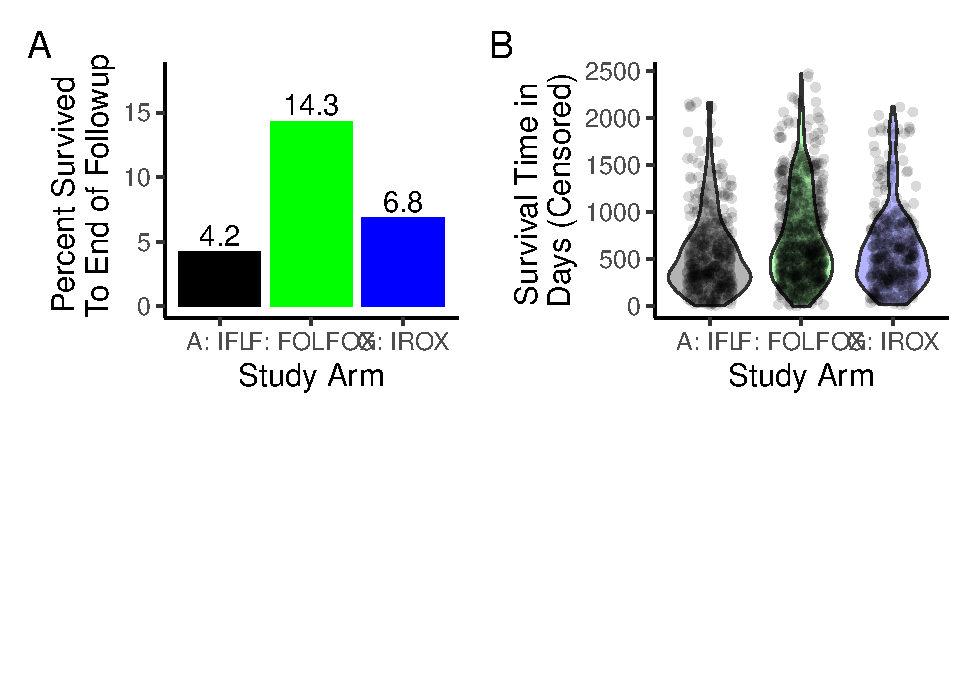
\includegraphics{io28-mockstudy_analysis_chisq_files/figure-latex/survivaltime_boxplot-1.pdf}

\hypertarget{now-add-a-survival-curve}{%
\subsection{Now add a survival curve}\label{now-add-a-survival-curve}}

For some reason, patchwork does not work with this survival curve

\begin{Shaded}
\begin{Highlighting}[]
\KeywordTok{survfit}\NormalTok{(}\DataTypeTok{formula =} \KeywordTok{Surv}\NormalTok{(fu.time, fu.stat) }\OperatorTok{~}\StringTok{ }\NormalTok{arm, }\DataTypeTok{data=}\NormalTok{ mockstudy) ->}
\NormalTok{fit}

\KeywordTok{ggsurvplot}\NormalTok{(fit,}
           \DataTypeTok{pval =} \OtherTok{TRUE}\NormalTok{, }\DataTypeTok{conf.int =} \OtherTok{TRUE}\NormalTok{,}
           \DataTypeTok{risk.table =} \OtherTok{TRUE}\NormalTok{,}
           \DataTypeTok{risk.table.col =} \StringTok{"strata"}\NormalTok{,}
           \DataTypeTok{linetype =} \StringTok{"strata"}\NormalTok{,}
           \DataTypeTok{surv.median.line =} \StringTok{"hv"}\NormalTok{,}
           \DataTypeTok{ggtheme =} \KeywordTok{theme_bw}\NormalTok{(),}
           \DataTypeTok{palette =} \KeywordTok{c}\NormalTok{(}\StringTok{"black"}\NormalTok{, }\StringTok{"blue"}\NormalTok{, }\StringTok{"gray80"}\NormalTok{)) }
\end{Highlighting}
\end{Shaded}

\begin{verbatim}
## Warning: Vectorized input to `element_text()` is not officially supported.
## Results may be unexpected or may change in future versions of ggplot2.
\end{verbatim}

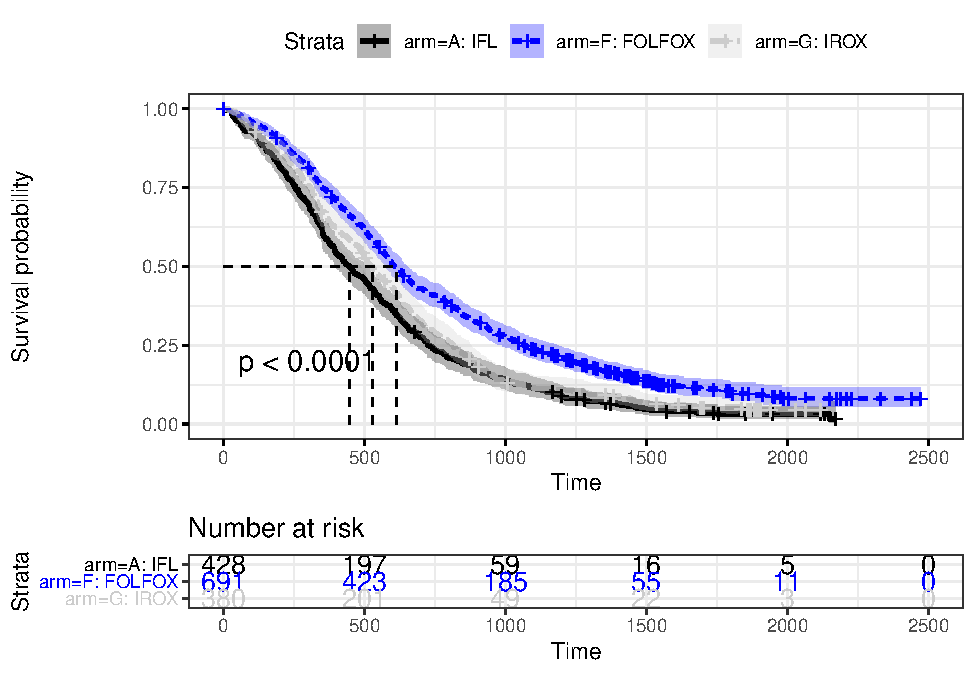
\includegraphics{io28-mockstudy_analysis_chisq_files/figure-latex/survival_curves-1.pdf}

\begin{Shaded}
\begin{Highlighting}[]
\NormalTok{mockstudy }\OperatorTok\StringTok{ }
\StringTok{  }\KeywordTok{tabyl}\NormalTok{(arm, fu.stat) }\OperatorTok\StringTok{ }
\StringTok{  }\KeywordTok{column_to_rownames}\NormalTok{(}\StringTok{'arm'}\NormalTok{) }\OperatorTok\StringTok{ }
\StringTok{  }\KeywordTok{chisq.test}\NormalTok{() ->}
\NormalTok{results}

\NormalTok{results}\OperatorTok{$}\NormalTok{statistic}
\end{Highlighting}
\end{Shaded}

\begin{verbatim}
## X-squared 
##  35.66764
\end{verbatim}

\begin{Shaded}
\begin{Highlighting}[]
\NormalTok{results}\OperatorTok{$}\NormalTok{parameter}
\end{Highlighting}
\end{Shaded}

\begin{verbatim}
## df 
##  2
\end{verbatim}

\hypertarget{study-results-1}{%
\section{Study Results}\label{study-results-1}}

This is an R Markdown document.

In the evaluation of followup status by study arm, the null hypothesis of independence was rejected, with a chi-squared statistic of 35.67, with 2 degrees of freedom, and a p value of 0, using the Pearson's Chi-squared test method.

\begin{verbatim}
## 
##  Pearson's Chi-squared test
## 
## data:  .
## X-squared = 1944.5, df = 36, p-value <
## 0.00000000000000022
\end{verbatim}

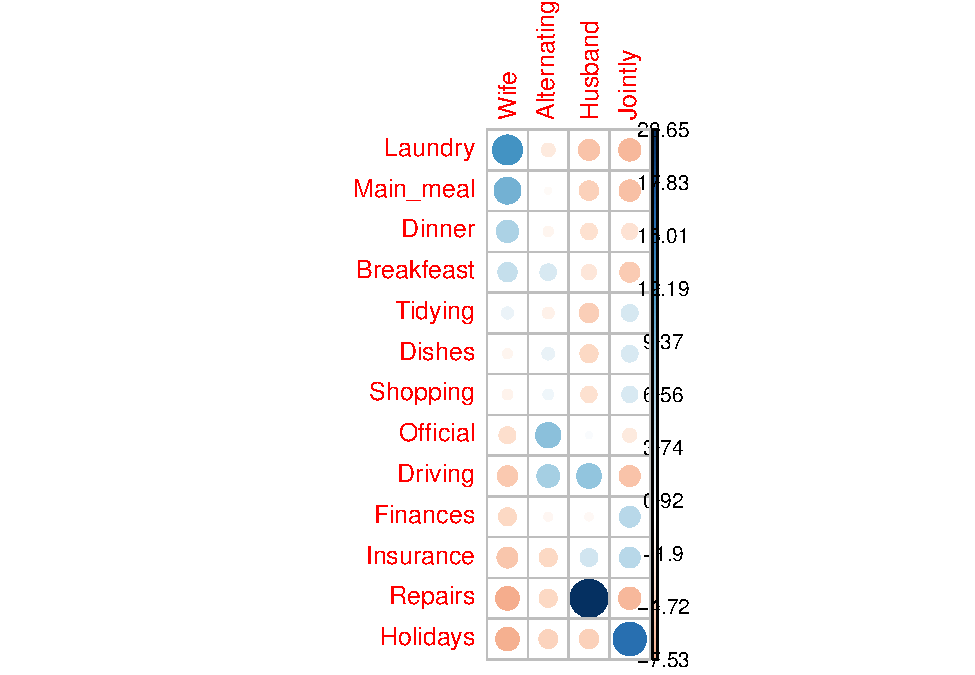
\includegraphics{io29a-chisq_example_files/figure-latex/corr-1.pdf}

In the evaluation of household tasks by person responsible, the null hypothesis of independence was rejected, with a chi-squared statistic of 1944.46, with 36 degrees of freedom, and a p value of 0, using the Pearson's Chi-squared test method.

\begin{Shaded}
\begin{Highlighting}[]
\NormalTok{housetasks }\OperatorTok\StringTok{ }
\StringTok{  }\KeywordTok{as.data.frame}\NormalTok{() }\OperatorTok\StringTok{ }
\StringTok{  }\KeywordTok{rownames_to_column}\NormalTok{(}\StringTok{"Task"}\NormalTok{) }\OperatorTok\StringTok{ }
\StringTok{  }\KeywordTok{filter}\NormalTok{(Task}\OperatorTok{==}\StringTok{"Finances"} \OperatorTok{|}\StringTok{ }\NormalTok{Task}\OperatorTok{==}\StringTok{"Official"}\NormalTok{) }\OperatorTok\StringTok{ }
\StringTok{  }\KeywordTok{select}\NormalTok{(Task, Wife, Husband) }\OperatorTok\StringTok{ }
\StringTok{  }\KeywordTok{column_to_rownames}\NormalTok{(}\StringTok{"Task"}\NormalTok{) }\OperatorTok\StringTok{ }
\StringTok{  }\KeywordTok{chisq.test}\NormalTok{()}
\end{Highlighting}
\end{Shaded}

\begin{verbatim}
## 
##  Pearson's Chi-squared test with Yates' continuity
##  correction
## 
## data:  .
## X-squared = 0.0082362, df = 1, p-value = 0.9277
\end{verbatim}

\begin{verbatim}
##             Wife Alternating Husband Jointly
## Laundry    7.738       0.272   1.777   2.246
## Main_meal  4.976       0.012   1.243   1.903
## Dinner     2.197       0.073   0.600   0.560
## Breakfeast 1.222       0.615   0.408   1.443
## Tidying    0.149       0.133   1.270   0.661
## Dishes     0.063       0.178   0.891   0.625
## Shopping   0.085       0.090   0.581   0.586
## Official   0.688       3.771   0.010   0.311
## Driving    1.538       2.403   3.374   1.789
## Finances   0.886       0.037   0.028   1.700
## Insurance  1.705       0.941   0.868   1.683
## Repairs    2.919       0.947  21.921   2.275
## Holidays   2.831       1.098   1.233  12.445
\end{verbatim}

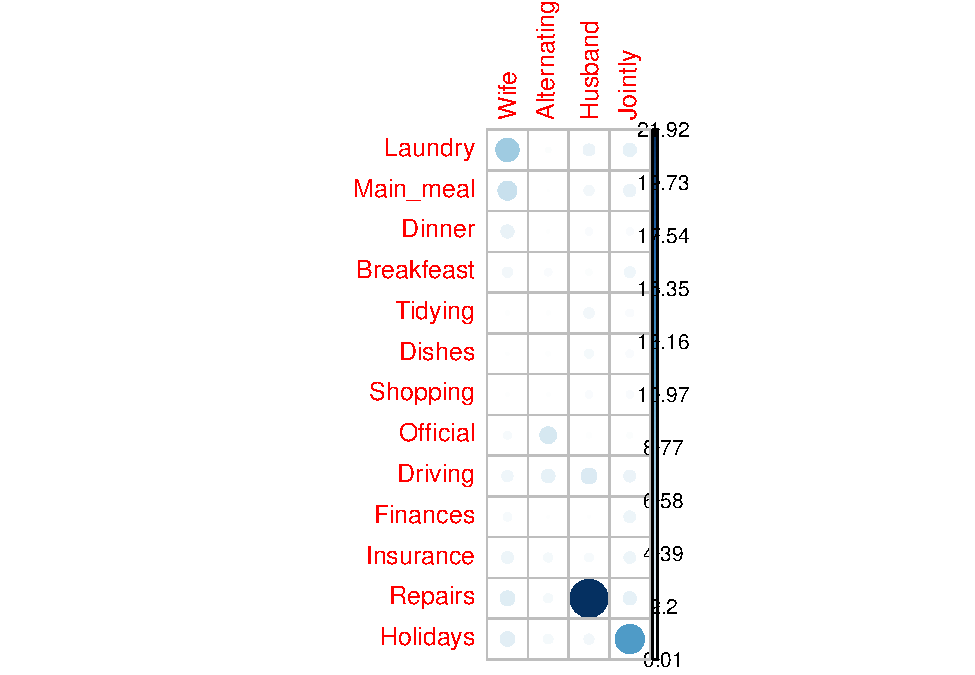
\includegraphics{io29a-chisq_example_files/figure-latex/percent-1.pdf}

\hypertarget{comparing-two-measures-of-centrality}{%
\section{Comparing Two Measures of Centrality}\label{comparing-two-measures-of-centrality}}

\begin{itemize}
\tightlist
\item
  Means and Medians
\item
  t tests and wilcoxon
\item
  for numerical continuous data
\end{itemize}

\hypertarget{common-problem}{%
\section{Common Problem}\label{common-problem}}

\begin{itemize}
\tightlist
\item
  Comparing two groups

  \begin{itemize}
  \tightlist
  \item
    Mean or median vs.~expected
  \item
    Two arms of study - independent
  \item
    Pre and post / spouse and partner / left vs right arm -- paired groups
  \end{itemize}
\item
  Are the means significantly different?
\item
  Or the medians (if not normally distributed)?
\end{itemize}

\hypertarget{how-skewed-is-too-skewed}{%
\section{How Skewed is Too Skewed?}\label{how-skewed-is-too-skewed}}

\begin{itemize}
\tightlist
\item
  Formal test of normality = Shapiro-Wilk test
\item
  Use base data set called ToothGrowth
\end{itemize}

\begin{Shaded}
\begin{Highlighting}[]
\KeywordTok{library}\NormalTok{(tidyverse)}
\NormalTok{data <-}\StringTok{ }\NormalTok{ToothGrowth}
\KeywordTok{head}\NormalTok{(data)}
\end{Highlighting}
\end{Shaded}

\begin{verbatim}
##    len supp dose
## 1  4.2   VC  0.5
## 2 11.5   VC  0.5
## 3  7.3   VC  0.5
## 4  5.8   VC  0.5
## 5  6.4   VC  0.5
## 6 10.0   VC  0.5
\end{verbatim}

\hypertarget{visualize-the-distribution-of-datalen-in-ggplot}{%
\section{Visualize the Distribution of data\$len in ggplot}\label{visualize-the-distribution-of-datalen-in-ggplot}}

\begin{itemize}
\tightlist
\item
  Use geom\_histogram or geom\_density
\item
  Bonus points: facet by supplement treatment
\item
  Your turn to try it
\end{itemize}

\includegraphics{io30-ttest_files/figure-latex/density-1.pdf}

\begin{Shaded}
\begin{Highlighting}[]
\NormalTok{data }\OperatorTok\StringTok{ }
\KeywordTok{ggplot}\NormalTok{(}\DataTypeTok{mapping =} \KeywordTok{aes}\NormalTok{(len)) }\OperatorTok{+}
\StringTok{  }\KeywordTok{geom_histogram}\NormalTok{() }\OperatorTok{+}
\StringTok{  }\CommentTok{#geom_density() + }
\StringTok{  }\KeywordTok{facet_wrap}\NormalTok{(}\OperatorTok{~}\NormalTok{supp)}
\end{Highlighting}
\end{Shaded}

\includegraphics{io30-ttest_files/figure-latex/histogram-1.pdf}

\hypertarget{visualize-the-distribution-of-datalen-in-ggplot-1}{%
\section{Visualize the Distribution of data\$len in ggplot}\label{visualize-the-distribution-of-datalen-in-ggplot-1}}

\begin{itemize}
\tightlist
\item
  The OJ group is left skewed
\item
  May be problematic for using means
\item
  formally test with Shapiro-Wilk
\end{itemize}

\begin{Shaded}
\begin{Highlighting}[]
\NormalTok{data}\OperatorTok{$}\NormalTok{len }\OperatorTok\StringTok{ }
\KeywordTok{shapiro.test}\NormalTok{()}
\end{Highlighting}
\end{Shaded}

\begin{verbatim}
## 
##  Shapiro-Wilk normality test
## 
## data:  .
## W = 0.96743, p-value = 0.1091
\end{verbatim}

\hypertarget{results-of-shapiro-wilk}{%
\section{Results of Shapiro-Wilk}\label{results-of-shapiro-wilk}}

\begin{itemize}
\tightlist
\item
  p-value = 0.1091
\item
  p not \textless{} 0.05
\item
  Acceptably close to normal
\item
  OK to compare means rather than medians
\item
  can use t test rather than wilcoxon test

  \begin{itemize}
  \tightlist
  \item
    if p is \textless{} 0.05, use wilcoxon test
  \item
    also known as Mann-Whitney test
  \item
    a rank-based (non-parametric) test
  \end{itemize}
\end{itemize}

\hypertarget{try-it-yourself}{%
\section{Try it yourself}\label{try-it-yourself}}

\begin{itemize}
\tightlist
\item
  use df \textless- msleep
\end{itemize}

\begin{Shaded}
\begin{Highlighting}[]
\NormalTok{df <-}\StringTok{ }\NormalTok{msleep }
\KeywordTok{head}\NormalTok{(df}\OperatorTok{$}\NormalTok{sleep_total)}
\end{Highlighting}
\end{Shaded}

\begin{verbatim}
## [1] 12.1 17.0 14.4 14.9  4.0 14.4
\end{verbatim}

\begin{itemize}
\tightlist
\item
  test the normality of total sleep hours in mammals
\end{itemize}

\hypertarget{mammal-sleep-hours}{%
\section{Mammal sleep hours}\label{mammal-sleep-hours}}

\begin{Shaded}
\begin{Highlighting}[]
\KeywordTok{shapiro.test}\NormalTok{(df}\OperatorTok{$}\NormalTok{sleep_total)}
\end{Highlighting}
\end{Shaded}

\begin{verbatim}
## 
##  Shapiro-Wilk normality test
## 
## data:  df$sleep_total
## W = 0.97973, p-value = 0.2143
\end{verbatim}

\begin{itemize}
\tightlist
\item
  meets criteria - acceptable to consider normally distributed
\item
  now consider - is the mean roughly 8 hours of sleep per day?
\end{itemize}

\hypertarget{one-sample-t-test}{%
\section{One Sample T test}\label{one-sample-t-test}}

\begin{itemize}
\tightlist
\item
  univariate test

  \begin{itemize}
  \tightlist
  \item
    Ho: mean is 8 hours
  \item
    Ha: mean is not 8 hours
  \end{itemize}
\item
  can use t test because shapiro.test is NS
\end{itemize}

\hypertarget{how-to-do-one-sample-t-test}{%
\section{How to do One Sample T test}\label{how-to-do-one-sample-t-test}}

\begin{Shaded}
\begin{Highlighting}[]
\KeywordTok{t.test}\NormalTok{(df}\OperatorTok{$}\NormalTok{sleep_total, }\DataTypeTok{alternative =} \StringTok{"two.sided"}\NormalTok{,}
       \DataTypeTok{mu =} \DecValTok{8}\NormalTok{)}
\end{Highlighting}
\end{Shaded}

\begin{itemize}
\tightlist
\item
  Try it out, see if you can interpret results
\end{itemize}

\hypertarget{interpreting-the-one-sample-t-test}{%
\section{Interpreting the One Sample T test}\label{interpreting-the-one-sample-t-test}}

\begin{verbatim}
## 
##  One Sample t-test
## 
## data:  df$sleep_total
## t = 4.9822, df = 82, p-value = 0.000003437
## alternative hypothesis: true mean is not equal to 8
## 95 percent confidence interval:
##   9.461972 11.405497
## sample estimates:
## mean of x 
##  10.43373
\end{verbatim}

\begin{itemize}
\tightlist
\item
  p is highly significant

  \begin{itemize}
  \tightlist
  \item
    can reject the null, accept alternative
  \item
    sample mean 10.43, CI 9.46-11.41
  \end{itemize}
\end{itemize}

\hypertarget{what-are-the-arguments-of-the-t.test-function}{%
\section{What are the arguments of the t.test function?}\label{what-are-the-arguments-of-the-t.test-function}}

\begin{itemize}
\tightlist
\item
  x = vector of continuous numerical data
\item
  y= NULL - optional 2nd vector of continuous numerical data
\item
  alternative = c(``two.sided'', ``less'', ``greater''),
\item
  mu = 0
\item
  paired = FALSE
\item
  var.equal = FALSE
\item
  conf.level = 0.95
\item
  \href{https://www.rdocumentation.org/packages/stats/versions/3.5.1/topics/t.test}{documentation}
\end{itemize}

\hypertarget{fine-but-what-about-2-groups}{%
\section{Fine, but what about 2 groups?}\label{fine-but-what-about-2-groups}}

\begin{itemize}
\tightlist
\item
  consider df\$vore
\end{itemize}

\begin{Shaded}
\begin{Highlighting}[]
\KeywordTok{table}\NormalTok{(df}\OperatorTok{$}\NormalTok{vore)}
\end{Highlighting}
\end{Shaded}

\begin{verbatim}
## 
##   carni   herbi insecti    omni 
##      19      32       5      20
\end{verbatim}

\begin{itemize}
\tightlist
\item
  hypothesis - herbivores need more time to get food, sleep less than carnivores
\item
  how to test this?

  \begin{itemize}
  \tightlist
  \item
    normal, so can use t test for 2 groups
  \end{itemize}
\end{itemize}

\hypertarget{setting-up-2-group-t-test}{%
\section{Setting up 2 group t test}\label{setting-up-2-group-t-test}}

\begin{itemize}
\tightlist
\item
  formula interface: outcome \textasciitilde{} groupvar
\end{itemize}

\begin{Shaded}
\begin{Highlighting}[]
\NormalTok{df }\OperatorTok\StringTok{ }
\StringTok{  }\KeywordTok{filter}\NormalTok{(vore }\OperatorTok\StringTok{ }\KeywordTok{c}\NormalTok{(}\StringTok{"herbi"}\NormalTok{, }\StringTok{"carni"}\NormalTok{)) }\OperatorTok\StringTok{ }
\StringTok{  }\KeywordTok{t.test}\NormalTok{(}\DataTypeTok{formula =}\NormalTok{ sleep_total }\OperatorTok{~}\StringTok{ }\NormalTok{vore, }\DataTypeTok{data =}\NormalTok{ .)}
\end{Highlighting}
\end{Shaded}

\begin{itemize}
\tightlist
\item
  Try it yourself
\item
  What do the results mean?
\end{itemize}

\hypertarget{results-of-the-2-group-t-test}{%
\section{Results of the 2 group t test}\label{results-of-the-2-group-t-test}}

\begin{verbatim}
## 
##  Welch Two Sample t-test
## 
## data:  sleep_total by vore
## t = 0.63232, df = 39.31, p-value = 0.5308
## alternative hypothesis: true difference in means is not equal to 0
## 95 percent confidence interval:
##  -1.911365  3.650509
## sample estimates:
## mean in group carni mean in group herbi 
##           10.378947            9.509375
\end{verbatim}

\hypertarget{interpreting-the-2-group-t-test}{%
\section{Interpreting the 2 group t test}\label{interpreting-the-2-group-t-test}}

\begin{itemize}
\tightlist
\item
  Welch t-test (not Student)

  \begin{itemize}
  \tightlist
  \item
    Welch does NOT assume equal variances in each group
  \end{itemize}
\item
  p value NS
\item
  accept null hypothesis

  \begin{itemize}
  \tightlist
  \item
    Ho: means of groups roughly equal
  \item
    Ha: means are different
  \item
    95\% CI crosses 0
  \end{itemize}
\item
  Carnivores sleep a little more, but not a lot
\end{itemize}

\hypertarget{group-t-test-with-wide-data}{%
\section{2 group t test with wide data}\label{group-t-test-with-wide-data}}

\begin{itemize}
\tightlist
\item
  You want to compare column A with column B (data are not tidy)
\item
  Do mammals spend more time awake than asleep?
\end{itemize}

\begin{Shaded}
\begin{Highlighting}[]
\KeywordTok{t.test}\NormalTok{(}\DataTypeTok{x =}\NormalTok{ df}\OperatorTok{$}\NormalTok{sleep_total, }\DataTypeTok{y =}\NormalTok{ df}\OperatorTok{$}\NormalTok{awake, }\DataTypeTok{data =}\NormalTok{ msleep)}
\end{Highlighting}
\end{Shaded}

\hypertarget{results-of-2-group-t-test-with-wide-data}{%
\section{Results of 2 group t test with wide data}\label{results-of-2-group-t-test-with-wide-data}}

\begin{Shaded}
\begin{Highlighting}[]
\KeywordTok{t.test}\NormalTok{(}\DataTypeTok{x =}\NormalTok{ df}\OperatorTok{$}\NormalTok{sleep_total, }\DataTypeTok{y =}\NormalTok{ df}\OperatorTok{$}\NormalTok{awake, }\DataTypeTok{data =}\NormalTok{ msleep)}
\end{Highlighting}
\end{Shaded}

\begin{verbatim}
## 
##  Welch Two Sample t-test
## 
## data:  df$sleep_total and df$awake
## t = -4.5353, df = 164, p-value = 0.00001106
## alternative hypothesis: true difference in means is not equal to 0
## 95 percent confidence interval:
##  -4.498066 -1.769404
## sample estimates:
## mean of x mean of y 
##  10.43373  13.56747
\end{verbatim}

\hypertarget{assumptions-of-students-t-test}{%
\section{3 Assumptions of Student's t test}\label{assumptions-of-students-t-test}}

\begin{enumerate}
\def\labelenumi{\arabic{enumi}.}
\tightlist
\item
  Sample is normally distributed (test with Shapiro)
\item
  Variances are homogeneous (homoskedasticity) (test with Levene)
\item
  Observations are independent
\end{enumerate}

\begin{itemize}
\tightlist
\item
  not paired like left vs.~right colon
\item
  not paired like spouse and partner
\item
  not paired like measurements pre and post Rx
\end{itemize}

\hypertarget{testing-assumptions-of-students-t-test}{%
\section{Testing Assumptions of Student's t test}\label{testing-assumptions-of-students-t-test}}

\begin{itemize}
\tightlist
\item
  Normality - test with Shapiro

  \begin{itemize}
  \tightlist
  \item
    If not normal, Wilcoxon \textgreater{} t test
  \end{itemize}
\item
  Equal Variances - test with Levene

  \begin{itemize}
  \tightlist
  \item
    If not equal, Welch t \textgreater{} Student's t
  \end{itemize}
\item
  Observations are independent

  \begin{itemize}
  \tightlist
  \item
    Think about data collection
  \item
    are some observations correlated with some others?
  \item
    If correlated, use paired t test
  \end{itemize}
\end{itemize}

\hypertarget{getting-results-out-of-t.test}{%
\section{Getting results out of t.test}\label{getting-results-out-of-t.test}}

\begin{itemize}
\tightlist
\item
  Use the tidy function from the broom package
\item
  Do carnivores have bigger brains than insectivores?
\end{itemize}

\begin{Shaded}
\begin{Highlighting}[]
\NormalTok{df }\OperatorTok\StringTok{ }
\StringTok{  }\KeywordTok{filter}\NormalTok{(vore }\OperatorTok\StringTok{ }\KeywordTok{c}\NormalTok{(}\StringTok{"carni"}\NormalTok{, }\StringTok{"insecti"}\NormalTok{)) }\OperatorTok\StringTok{ }
\KeywordTok{t.test}\NormalTok{(}\DataTypeTok{formula =}\NormalTok{ brainwt }\OperatorTok{~}\StringTok{ }\NormalTok{vore, }\DataTypeTok{data =}\NormalTok{ .) }\OperatorTok\StringTok{ }
\StringTok{  }\KeywordTok{tidy}\NormalTok{() ->}
\NormalTok{result}
\NormalTok{result}
\end{Highlighting}
\end{Shaded}

\hypertarget{getting-results-out-of-t.test-1}{%
\section{Getting results out of t.test}\label{getting-results-out-of-t.test-1}}

\begin{verbatim}
## # A tibble: 1 x 9
##   estimate1 estimate2 statistic p.value parameter conf.low
##       <dbl>     <dbl>     <dbl>   <dbl>     <dbl>    <dbl>
## 1    0.0793    0.0216      1.20   0.253        12  -0.0471
## # ... with 3 more variables: conf.high <dbl>, method <chr>,
## #   alternative <chr>
\end{verbatim}

\hypertarget{reporting-the-results-from-t.test-using-inline-code}{%
\section{Reporting the results from t.test using inline code}\label{reporting-the-results-from-t.test-using-inline-code}}

\begin{itemize}
\tightlist
\item
  use backticks before and after, start with r

  \begin{itemize}
  \tightlist
  \item
    i.e.~My result is {[}backtick{]}r code here{[}backtick{]}.
  \end{itemize}
\item
  The mean brain weight for carnivores was 0.0792556
\item
  The mean brain weight for herbivores was 0.02155

  \begin{itemize}
  \tightlist
  \item
    The difference was
  \end{itemize}
\item
  The t statistic for this Two Sample t-test was 1.1995501
\item
  The p value was 0.2534631

  \begin{itemize}
  \tightlist
  \item
    The confidence interval was from -0.05 to 0.16
  \end{itemize}
\end{itemize}

\hypertarget{for-next-time}{%
\section{For Next Time}\label{for-next-time}}

\begin{itemize}
\tightlist
\item
  Skewness and Kurtosis
\item
  Review Normality

  \begin{itemize}
  \tightlist
  \item
    When to use Wilcoxon
  \end{itemize}
\item
  Levene test for equal variances

  \begin{itemize}
  \tightlist
  \item
    When to use Welch t vs.~Student's t
  \end{itemize}
\item
  Paired t and Wilcoxon tests
\end{itemize}

\hypertarget{comparing-two-measures-of-centrality-1}{%
\section{Comparing Two Measures of Centrality}\label{comparing-two-measures-of-centrality-1}}

\begin{itemize}
\tightlist
\item
  Means and Medians
\item
  t tests and wilcoxon
\item
  for numerical continuous data
\end{itemize}

\hypertarget{common-problem-1}{%
\section{Common Problem}\label{common-problem-1}}

\begin{itemize}
\tightlist
\item
  Comparing two groups

  \begin{itemize}
  \tightlist
  \item
    Mean or median vs.~expected
  \item
    Two arms of study - independent
  \item
    Pre and post / spouse and partner / left vs right arm -- paired groups
  \end{itemize}
\item
  Are the means significantly different?
\item
  Or the medians (if not normally distributed)?
\end{itemize}

\hypertarget{how-skewed-is-too-skewed-1}{%
\section{How Skewed is Too Skewed?}\label{how-skewed-is-too-skewed-1}}

\begin{itemize}
\tightlist
\item
  Formal test of normality = Shapiro-Wilk test
\item
  Use base data set called ToothGrowth
\end{itemize}

\begin{Shaded}
\begin{Highlighting}[]
\KeywordTok{library}\NormalTok{(tidyverse)}
\NormalTok{data <-}\StringTok{ }\NormalTok{ToothGrowth}
\KeywordTok{head}\NormalTok{(data)}
\end{Highlighting}
\end{Shaded}

\begin{verbatim}
##    len supp dose
## 1  4.2   VC  0.5
## 2 11.5   VC  0.5
## 3  7.3   VC  0.5
## 4  5.8   VC  0.5
## 5  6.4   VC  0.5
## 6 10.0   VC  0.5
\end{verbatim}

\hypertarget{visualize-the-distribution-of-datalen-in-ggplot-2}{%
\section{Visualize the Distribution of data\$len in ggplot}\label{visualize-the-distribution-of-datalen-in-ggplot-2}}

\begin{itemize}
\tightlist
\item
  Use geom\_histogram or geom\_density
\item
  Bonus points: facet by supplement treatment
\item
  Your turn to try it
\end{itemize}

\includegraphics{io30a-ttest_files/figure-latex/density-1.pdf}

\begin{Shaded}
\begin{Highlighting}[]
\NormalTok{data }\OperatorTok\StringTok{ }
\KeywordTok{ggplot}\NormalTok{(}\DataTypeTok{mapping =} \KeywordTok{aes}\NormalTok{(len)) }\OperatorTok{+}
\StringTok{  }\KeywordTok{geom_histogram}\NormalTok{() }\OperatorTok{+}
\StringTok{  }\CommentTok{#geom_density() + }
\StringTok{  }\KeywordTok{facet_wrap}\NormalTok{(}\OperatorTok{~}\NormalTok{supp)}
\end{Highlighting}
\end{Shaded}

\includegraphics{io30a-ttest_files/figure-latex/histogram-1.pdf}

\hypertarget{visualize-the-distribution-of-datalen-in-ggplot-3}{%
\section{Visualize the Distribution of data\$len in ggplot}\label{visualize-the-distribution-of-datalen-in-ggplot-3}}

\begin{itemize}
\tightlist
\item
  The OJ group is left skewed
\item
  May be problematic for using means
\item
  formally test with Shapiro-Wilk
\end{itemize}

\begin{Shaded}
\begin{Highlighting}[]
\NormalTok{data}\OperatorTok{$}\NormalTok{len }\OperatorTok\StringTok{ }
\KeywordTok{shapiro.test}\NormalTok{()}
\end{Highlighting}
\end{Shaded}

\begin{verbatim}
## 
##  Shapiro-Wilk normality test
## 
## data:  .
## W = 0.96743, p-value = 0.1091
\end{verbatim}

\hypertarget{results-of-shapiro-wilk-1}{%
\section{Results of Shapiro-Wilk}\label{results-of-shapiro-wilk-1}}

\begin{itemize}
\tightlist
\item
  p-value = 0.1091
\item
  p not \textless{} 0.05
\item
  Acceptably close to normal
\item
  OK to compare means rather than medians
\item
  can use t test rather than wilcoxon test

  \begin{itemize}
  \tightlist
  \item
    if p is \textless{} 0.05, use wilcoxon test
  \item
    also known as Mann-Whitney test
  \item
    a rank-based (non-parametric) test
  \end{itemize}
\end{itemize}

\hypertarget{try-it-yourself-1}{%
\section{Try it yourself}\label{try-it-yourself-1}}

\begin{itemize}
\tightlist
\item
  use df \textless- msleep
\end{itemize}

\begin{Shaded}
\begin{Highlighting}[]
\NormalTok{df <-}\StringTok{ }\NormalTok{msleep }
\KeywordTok{head}\NormalTok{(df}\OperatorTok{$}\NormalTok{sleep_total)}
\end{Highlighting}
\end{Shaded}

\begin{verbatim}
## [1] 12.1 17.0 14.4 14.9  4.0 14.4
\end{verbatim}

\begin{itemize}
\tightlist
\item
  test the normality of total sleep hours in mammals
\end{itemize}

\hypertarget{mammal-sleep-hours-1}{%
\section{Mammal sleep hours}\label{mammal-sleep-hours-1}}

\begin{Shaded}
\begin{Highlighting}[]
\KeywordTok{shapiro.test}\NormalTok{(df}\OperatorTok{$}\NormalTok{sleep_total)}
\end{Highlighting}
\end{Shaded}

\begin{verbatim}
## 
##  Shapiro-Wilk normality test
## 
## data:  df$sleep_total
## W = 0.97973, p-value = 0.2143
\end{verbatim}

\begin{itemize}
\tightlist
\item
  meets criteria - acceptable to consider normally distributed
\item
  now consider - is the mean roughly 8 hours of sleep per day?
\end{itemize}

\hypertarget{one-sample-t-test-1}{%
\section{One Sample T test}\label{one-sample-t-test-1}}

\begin{itemize}
\tightlist
\item
  univariate test

  \begin{itemize}
  \tightlist
  \item
    Ho: mean is 8 hours
  \item
    Ha: mean is not 8 hours
  \end{itemize}
\item
  can use t test because shapiro.test is NS
\end{itemize}

\hypertarget{how-to-do-one-sample-t-test-1}{%
\section{How to do One Sample T test}\label{how-to-do-one-sample-t-test-1}}

\begin{Shaded}
\begin{Highlighting}[]
\KeywordTok{t.test}\NormalTok{(df}\OperatorTok{$}\NormalTok{sleep_total, }\DataTypeTok{alternative =} \StringTok{"two.sided"}\NormalTok{,}
       \DataTypeTok{mu =} \DecValTok{8}\NormalTok{)}
\end{Highlighting}
\end{Shaded}

\begin{itemize}
\tightlist
\item
  Try it out, see if you can interpret results
\end{itemize}

\hypertarget{interpreting-the-one-sample-t-test-1}{%
\section{Interpreting the One Sample T test}\label{interpreting-the-one-sample-t-test-1}}

\begin{verbatim}
## 
##  One Sample t-test
## 
## data:  df$sleep_total
## t = 4.9822, df = 82, p-value = 0.000003437
## alternative hypothesis: true mean is not equal to 8
## 95 percent confidence interval:
##   9.461972 11.405497
## sample estimates:
## mean of x 
##  10.43373
\end{verbatim}

\begin{itemize}
\tightlist
\item
  p is highly significant

  \begin{itemize}
  \tightlist
  \item
    can reject the null, accept alternative
  \item
    sample mean 10.43, CI 9.46-11.41
  \end{itemize}
\end{itemize}

\hypertarget{what-are-the-arguments-of-the-t.test-function-1}{%
\section{What are the arguments of the t.test function?}\label{what-are-the-arguments-of-the-t.test-function-1}}

\begin{itemize}
\tightlist
\item
  x = vector of continuous numerical data
\item
  y= NULL - optional 2nd vector of continuous numerical data
\item
  alternative = c(``two.sided'', ``less'', ``greater''),
\item
  mu = 0
\item
  paired = FALSE
\item
  var.equal = FALSE
\item
  conf.level = 0.95
\item
  \href{https://www.rdocumentation.org/packages/stats/versions/3.5.1/topics/t.test}{documentation}
\end{itemize}

\hypertarget{fine-but-what-about-2-groups-1}{%
\section{Fine, but what about 2 groups?}\label{fine-but-what-about-2-groups-1}}

\begin{itemize}
\tightlist
\item
  consider df\$vore
\end{itemize}

\begin{Shaded}
\begin{Highlighting}[]
\KeywordTok{table}\NormalTok{(df}\OperatorTok{$}\NormalTok{vore)}
\end{Highlighting}
\end{Shaded}

\begin{verbatim}
## 
##   carni   herbi insecti    omni 
##      19      32       5      20
\end{verbatim}

\begin{itemize}
\tightlist
\item
  hypothesis - herbivores need more time to get food, sleep less than carnivores
\item
  how to test this?

  \begin{itemize}
  \tightlist
  \item
    normal, so can use t test for 2 groups
  \end{itemize}
\end{itemize}

\hypertarget{setting-up-2-group-t-test-1}{%
\section{Setting up 2 group t test}\label{setting-up-2-group-t-test-1}}

\begin{itemize}
\tightlist
\item
  formula interface: outcome \textasciitilde{} groupvar
\end{itemize}

\begin{Shaded}
\begin{Highlighting}[]
\NormalTok{df }\OperatorTok\StringTok{ }
\StringTok{  }\KeywordTok{filter}\NormalTok{(vore }\OperatorTok\StringTok{ }\KeywordTok{c}\NormalTok{(}\StringTok{"herbi"}\NormalTok{, }\StringTok{"carni"}\NormalTok{)) }\OperatorTok\StringTok{ }
\StringTok{  }\KeywordTok{t.test}\NormalTok{(}\DataTypeTok{formula =}\NormalTok{ sleep_total }\OperatorTok{~}\StringTok{ }\NormalTok{vore, }\DataTypeTok{data =}\NormalTok{ .)}
\end{Highlighting}
\end{Shaded}

\begin{itemize}
\tightlist
\item
  Try it yourself
\item
  What do the results mean?
\end{itemize}

\hypertarget{results-of-the-2-group-t-test-1}{%
\section{Results of the 2 group t test}\label{results-of-the-2-group-t-test-1}}

\begin{verbatim}
## 
##  Welch Two Sample t-test
## 
## data:  sleep_total by vore
## t = 0.63232, df = 39.31, p-value = 0.5308
## alternative hypothesis: true difference in means is not equal to 0
## 95 percent confidence interval:
##  -1.911365  3.650509
## sample estimates:
## mean in group carni mean in group herbi 
##           10.378947            9.509375
\end{verbatim}

\hypertarget{interpreting-the-2-group-t-test-1}{%
\section{Interpreting the 2 group t test}\label{interpreting-the-2-group-t-test-1}}

\begin{itemize}
\tightlist
\item
  Welch t-test (not Student)

  \begin{itemize}
  \tightlist
  \item
    Welch does NOT assume equal variances in each group
  \end{itemize}
\item
  p value NS
\item
  accept null hypothesis

  \begin{itemize}
  \tightlist
  \item
    Ho: means of groups roughly equal
  \item
    Ha: means are different
  \item
    95\% CI crosses 0
  \end{itemize}
\item
  Carnivores sleep a little more, but not a lot
\end{itemize}

\hypertarget{group-t-test-with-wide-data-1}{%
\section{2 group t test with wide data}\label{group-t-test-with-wide-data-1}}

\begin{itemize}
\tightlist
\item
  You want to compare column A with column B (data are not tidy)
\item
  Do mammals spend more time awake than asleep?
\end{itemize}

\begin{Shaded}
\begin{Highlighting}[]
\KeywordTok{t.test}\NormalTok{(}\DataTypeTok{x =}\NormalTok{ df}\OperatorTok{$}\NormalTok{sleep_total, }\DataTypeTok{y =}\NormalTok{ df}\OperatorTok{$}\NormalTok{awake, }\DataTypeTok{data =}\NormalTok{ msleep)}
\end{Highlighting}
\end{Shaded}

\hypertarget{results-of-2-group-t-test-with-wide-data-1}{%
\section{Results of 2 group t test with wide data}\label{results-of-2-group-t-test-with-wide-data-1}}

\begin{Shaded}
\begin{Highlighting}[]
\KeywordTok{t.test}\NormalTok{(}\DataTypeTok{x =}\NormalTok{ df}\OperatorTok{$}\NormalTok{sleep_total, }\DataTypeTok{y =}\NormalTok{ df}\OperatorTok{$}\NormalTok{awake, }\DataTypeTok{data =}\NormalTok{ msleep)}
\end{Highlighting}
\end{Shaded}

\begin{verbatim}
## 
##  Welch Two Sample t-test
## 
## data:  df$sleep_total and df$awake
## t = -4.5353, df = 164, p-value = 0.00001106
## alternative hypothesis: true difference in means is not equal to 0
## 95 percent confidence interval:
##  -4.498066 -1.769404
## sample estimates:
## mean of x mean of y 
##  10.43373  13.56747
\end{verbatim}

\hypertarget{assumptions-of-students-t-test-1}{%
\section{3 Assumptions of Student's t test}\label{assumptions-of-students-t-test-1}}

\begin{enumerate}
\def\labelenumi{\arabic{enumi}.}
\tightlist
\item
  Sample is normally distributed (test with Shapiro)
\item
  Variances are homogeneous (homoskedasticity) (test with Levene)
\item
  Observations are independent
\end{enumerate}

\begin{itemize}
\tightlist
\item
  not paired like left vs.~right colon
\item
  not paired like spouse and partner
\item
  not paired like measurements pre and post Rx
\end{itemize}

\hypertarget{testing-assumptions-of-students-t-test-1}{%
\section{Testing Assumptions of Student's t test}\label{testing-assumptions-of-students-t-test-1}}

\begin{itemize}
\tightlist
\item
  Normality - test with Shapiro

  \begin{itemize}
  \tightlist
  \item
    If not normal, Wilcoxon \textgreater{} t test
  \end{itemize}
\item
  Equal Variances - test with Levene

  \begin{itemize}
  \tightlist
  \item
    If not equal, Welch t \textgreater{} Student's t
  \end{itemize}
\item
  Observations are independent

  \begin{itemize}
  \tightlist
  \item
    Think about data collection
  \item
    are some observations correlated with some others?
  \item
    If correlated, use paired t test
  \end{itemize}
\end{itemize}

\hypertarget{getting-results-out-of-t.test-2}{%
\section{Getting results out of t.test}\label{getting-results-out-of-t.test-2}}

\begin{itemize}
\tightlist
\item
  Use the tidy function from the broom package
\item
  Do carnivores have bigger brains than insectivores?
\end{itemize}

\begin{Shaded}
\begin{Highlighting}[]
\NormalTok{df }\OperatorTok\StringTok{ }
\StringTok{  }\KeywordTok{filter}\NormalTok{(vore }\OperatorTok\StringTok{ }\KeywordTok{c}\NormalTok{(}\StringTok{"carni"}\NormalTok{, }\StringTok{"insecti"}\NormalTok{)) }\OperatorTok\StringTok{ }
\KeywordTok{t.test}\NormalTok{(}\DataTypeTok{formula =}\NormalTok{ brainwt }\OperatorTok{~}\StringTok{ }\NormalTok{vore, }\DataTypeTok{data =}\NormalTok{ .) }\OperatorTok\StringTok{ }
\StringTok{  }\KeywordTok{tidy}\NormalTok{() ->}
\NormalTok{result}
\NormalTok{result}
\end{Highlighting}
\end{Shaded}

\hypertarget{getting-results-out-of-t.test-3}{%
\section{Getting results out of t.test}\label{getting-results-out-of-t.test-3}}

\begin{verbatim}
## # A tibble: 1 x 9
##   estimate1 estimate2 statistic p.value parameter conf.low
##       <dbl>     <dbl>     <dbl>   <dbl>     <dbl>    <dbl>
## 1    0.0793    0.0216      1.20   0.253        12  -0.0471
## # ... with 3 more variables: conf.high <dbl>, method <chr>,
## #   alternative <chr>
\end{verbatim}

\hypertarget{reporting-the-results-from-t.test-using-inline-code-1}{%
\section{Reporting the results from t.test using inline code}\label{reporting-the-results-from-t.test-using-inline-code-1}}

\begin{itemize}
\tightlist
\item
  use backticks before and after, start with r

  \begin{itemize}
  \tightlist
  \item
    i.e.~My result is {[}backtick{]}r code here{[}backtick{]}.
  \end{itemize}
\item
  The mean brain weight for carnivores was 0.0792556
\item
  The mean brain weight for herbivores was 0.02155

  \begin{itemize}
  \tightlist
  \item
    The difference was
  \end{itemize}
\item
  The t statistic for this Two Sample t-test was 1.1995501
\item
  The p value was 0.2534631

  \begin{itemize}
  \tightlist
  \item
    The confidence interval was from -0.05 to 0.16
  \end{itemize}
\end{itemize}

\hypertarget{for-next-time-1}{%
\section{For Next Time}\label{for-next-time-1}}

\begin{itemize}
\tightlist
\item
  Skewness and Kurtosis
\item
  Review Normality

  \begin{itemize}
  \tightlist
  \item
    When to use Wilcoxon
  \end{itemize}
\item
  Levene test for equal variances

  \begin{itemize}
  \tightlist
  \item
    When to use Welch t vs.~Student's t
  \end{itemize}
\item
  Paired t and Wilcoxon tests
\end{itemize}

\hypertarget{review-from-t-test-part-1}{%
\section{Review from t test part 1}\label{review-from-t-test-part-1}}

\begin{itemize}
\tightlist
\item
  Comparing Two Measures of Centrality

  \begin{itemize}
  \tightlist
  \item
    is it normal (Shapiro test)?

    \begin{itemize}
    \tightlist
    \item
      if yes, use t test
    \item
      if no, use Wilcoxon rank test (nonparametric)
    \end{itemize}
  \item
    are the observations paired?

    \begin{itemize}
    \tightlist
    \item
      if yes, use paired Wilcoxon or paired t test
    \item
      if no, can use usual versions
    \end{itemize}
  \item
    are the variances equal in 2 groups (Levene test)?

    \begin{itemize}
    \tightlist
    \item
      if yes, OK to use Student's t test
    \item
      if no, must use Welch t test (unequal var)
    \end{itemize}
  \end{itemize}
\end{itemize}

\hypertarget{review-how-to-do-t-test-part-1}{%
\section{Review how to do t test part 1}\label{review-how-to-do-t-test-part-1}}

\begin{itemize}
\tightlist
\item
  one sample

  \begin{itemize}
  \tightlist
  \item
    t.test(df\$sleep\_total, alternative = ``two.sided'', mu = 8)
  \end{itemize}
\item
  formula interface: outcome \textasciitilde{} groupvar
  df \%\textgreater\% filter(vore \%in\% c(``herbi'', ``carni'')) \%\textgreater\% t.test(formula = sleep\_total \textasciitilde{} vore, data = .)
\item
  use broom::tidy() to get results into a dataframe
\item
  can use results in text with inline code
\item
  use backticks before and after, start with r
  i.e.~My result is {[}backtick{]}r code here{[}backtick{]}.
\end{itemize}

\hypertarget{what-we-have-left-to-cover}{%
\section{What We have Left to Cover}\label{what-we-have-left-to-cover}}

\begin{itemize}
\tightlist
\item
  General info on Skewness and Kurtosis
\item
  When to use t tests vs.~rank (wilcoxon)
\item
  Levene test for equal variances

  \begin{itemize}
  \tightlist
  \item
    When to use Welch t vs.~Student's t
  \end{itemize}
\item
  Paired t and Wilcoxon tests
\end{itemize}

\hypertarget{skewness}{%
\section{Skewness}\label{skewness}}

\begin{itemize}
\tightlist
\item
  A term for asymmetric data - obviously not normal
\item
  Left-skewed - long leftward tail
\item
  aka negatively skewed
  - mean less than the median
  - typical of age at death in US, number of questions answered on a survey, sq\_ft/\$ in Ann Arbor housing
  - often has a natural upper bound
\item
  Right-skewed - long rightward tail

  \begin{itemize}
  \tightlist
  \item
    aka positively skewed
  \item
    mean greater than the median
  \item
    typical of length of stay, medical costs, children per family
  \item
    mostly low, but some huge outliers
  \item
    often has a natural lower bound
  \end{itemize}
\end{itemize}

\hypertarget{skewness-example-old-faithful-geyser-eruption-duration}{%
\section{Skewness example: Old Faithful geyser eruption duration}\label{skewness-example-old-faithful-geyser-eruption-duration}}

\begin{itemize}
\tightlist
\item
  Duration of eruptions in minutes is negatively skewed
\end{itemize}

\begin{verbatim}
## 
## Attaching package: 'MASS'
\end{verbatim}

\begin{verbatim}
## The following object is masked from 'package:dplyr':
## 
##     select
\end{verbatim}

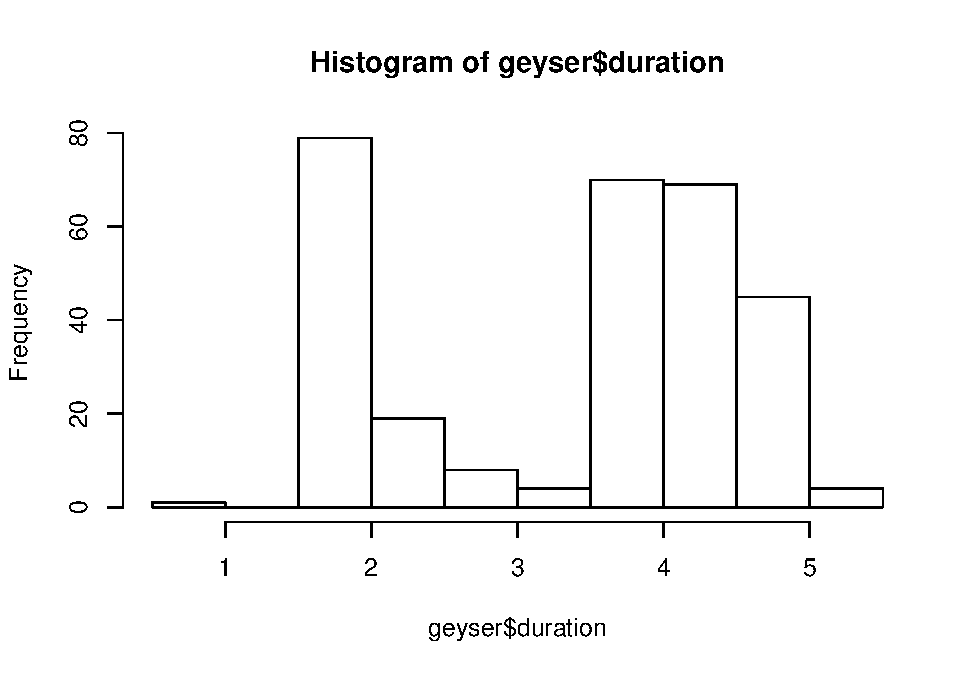
\includegraphics{io31-ttest_part2_files/figure-latex/geys-1.pdf}

\hypertarget{skewness-example-old-faithful-eruption-wait-times}{%
\section{Skewness example: Old Faithful eruption wait times}\label{skewness-example-old-faithful-eruption-wait-times}}

\begin{itemize}
\tightlist
\item
  Wait time for eruptions in minutes is negatively skewed
  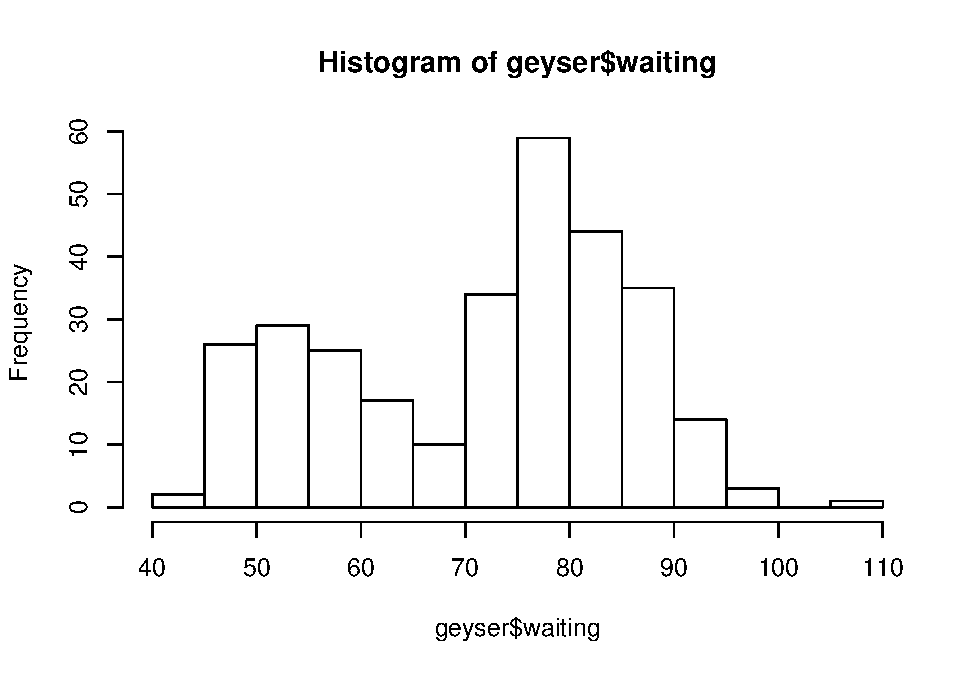
\includegraphics{io31-ttest_part2_files/figure-latex/geyser2-1.pdf}
  \#\# How Skewed is Too Skewed?
\item
  Formal test of normality = Shapiro-Wilk test
\item
  Use base data set called ToothGrowth
\item
  test the len variable
\end{itemize}

\begin{Shaded}
\begin{Highlighting}[]
\KeywordTok{library}\NormalTok{(tidyverse)}
\KeywordTok{library}\NormalTok{(MASS)}
\KeywordTok{shapiro.test}\NormalTok{(geyser}\OperatorTok{$}\NormalTok{waiting)}
\end{Highlighting}
\end{Shaded}

\begin{verbatim}
## 
##  Shapiro-Wilk normality test
## 
## data:  geyser$waiting
## W = 0.93871, p-value = 0.0000000008541
\end{verbatim}

\hypertarget{kurtosis}{%
\section{Kurtosis}\label{kurtosis}}

\begin{itemize}
\tightlist
\item
  Descriptive of how tightly bunched data are

  \begin{itemize}
  \tightlist
  \item
    leptokurtotic - histogram has tall peak, little spread

    \begin{itemize}
    \tightlist
    \item
      think leaping high = lepto
    \item
      values \textless3 are platykurtotic
    \end{itemize}
  \item
    platykurtotic - histogram is mostly flat, wide spread

    \begin{itemize}
    \tightlist
    \item
      think flat, like a platypus beak
    \item
      values \textless3 are platykurtotic
    \end{itemize}
  \item
    kurtosis values \textasciitilde{} 3 are mesokurtotic
  \end{itemize}
\end{itemize}

\begin{Shaded}
\begin{Highlighting}[]
\KeywordTok{library}\NormalTok{(tidyverse)}
\KeywordTok{library}\NormalTok{(MASS)}
\CommentTok{#kurtosis(geyser$waiting)}
\end{Highlighting}
\end{Shaded}

\hypertarget{decision-tree-for-comparing-2-group-data}{%
\section{Decision tree for Comparing 2 group data}\label{decision-tree-for-comparing-2-group-data}}

\begin{enumerate}
\def\labelenumi{\arabic{enumi}.}
\tightlist
\item
  Is it normal (Shapiro test)?
\end{enumerate}

\begin{itemize}
\tightlist
\item
  yes - t.test
\item
  no - wilcoxon
\end{itemize}

\begin{enumerate}
\def\labelenumi{\arabic{enumi}.}
\setcounter{enumi}{1}
\tightlist
\item
  Is it paired data?
\end{enumerate}

\begin{itemize}
\tightlist
\item
  use paired variants of either t.test or wilcoxon
\end{itemize}

\begin{enumerate}
\def\labelenumi{\arabic{enumi}.}
\setcounter{enumi}{2}
\tightlist
\item
  If normal, are the variances of the two groups equal (Levene test)?
\end{enumerate}

\begin{itemize}
\tightlist
\item
  if yes, use Student t test (var.equal=TRUE)
\item
  if no, use Welch t test (var.equal = FALSE)
\end{itemize}

\hypertarget{tooth-length-data}{%
\section{Tooth length data}\label{tooth-length-data}}

\begin{itemize}
\tightlist
\item
  We know it is reasonably normal from Shapiro test

  \begin{itemize}
  \tightlist
  \item
    Ok to use t test
  \end{itemize}
\item
  Should we use the Student version (var.equal) or the Welch version?

  \begin{itemize}
  \tightlist
  \item
    Welch (var.equal = FALSE) is the default
  \end{itemize}
\item
  Determine this with Levene test for 2 groups (in car package)

  \begin{itemize}
  \tightlist
  \item
    use Bartlett test if \textgreater2 groups and normally distributed
  \end{itemize}
\end{itemize}

\begin{Shaded}
\begin{Highlighting}[]
\KeywordTok{library}\NormalTok{(tidyverse)}
\KeywordTok{library}\NormalTok{(car)}
\NormalTok{data <-}\StringTok{ }\NormalTok{ToothGrowth}
\NormalTok{data }\OperatorTok\StringTok{ }
\StringTok{  }\KeywordTok{filter}\NormalTok{(dose }\OperatorTok{>}\StringTok{ }\FloatTok{0.9}\NormalTok{) }\OperatorTok\StringTok{ }
\StringTok{  }\KeywordTok{leveneTest}\NormalTok{(len }\OperatorTok{~}\StringTok{ }\KeywordTok{as.factor}\NormalTok{(dose), }\DataTypeTok{data =}\NormalTok{ .)}
\end{Highlighting}
\end{Shaded}

\begin{verbatim}
## Levene's Test for Homogeneity of Variance (center = median)
##       Df F value Pr(>F)
## group  1  1.6144 0.2116
##       38
\end{verbatim}

\begin{Shaded}
\begin{Highlighting}[]
\CommentTok{# note has to be as.factor - will not evaluate if groupvar is numeric}
\end{Highlighting}
\end{Shaded}

\hypertarget{interpretation-of-levenes-test}{%
\section{Interpretation of Levene's test}\label{interpretation-of-levenes-test}}

\begin{itemize}
\tightlist
\item
  the null hypothesis is that all populations variances are equal;
\item
  the alternative hypothesis is that at least two of them differ.
\end{itemize}

\begin{verbatim}
## Levene's Test for Homogeneity of Variance (center = median)
##       Df F value Pr(>F)
## group  1  1.6144 0.2116
##       38
\end{verbatim}

\begin{itemize}
\tightlist
\item
  will not reject null, OK to use Student t test
\end{itemize}

\hypertarget{arguments-for-t.test}{%
\section{Arguments for t.test}\label{arguments-for-t.test}}

x = vector of continuous numerical data
alternative = c(``two.sided'', ``less'', ``greater''),
mu = 0
paired = FALSE
var.equal = FALSE
conf.level = 0.95
Open the t.test help - type in console ``?t.test''

\hypertarget{mammal-sleep-hours-for-t-test}{%
\section{Mammal sleep hours for t test}\label{mammal-sleep-hours-for-t-test}}

First with Student t test, compare herbivores to omnivores by sleep\_rem

\begin{Shaded}
\begin{Highlighting}[]
\NormalTok{df <-}\StringTok{ }\NormalTok{msleep}
\NormalTok{df }\OperatorTok\StringTok{ }
\StringTok{  }\KeywordTok{filter}\NormalTok{(vore }\OperatorTok{!=}\StringTok{ 'carni'}\NormalTok{) }\OperatorTok\StringTok{ }
\StringTok{  }\KeywordTok{filter}\NormalTok{(vore }\OperatorTok{!=}\StringTok{ 'insecti'}\NormalTok{) }\OperatorTok\StringTok{ }
\StringTok{  }\KeywordTok{t.test}\NormalTok{(sleep_rem }\OperatorTok{~}\StringTok{ }\NormalTok{vore, }\DataTypeTok{data=}\NormalTok{., }\DataTypeTok{var.equal=}\OtherTok{TRUE}\NormalTok{)}
\end{Highlighting}
\end{Shaded}

\begin{verbatim}
## 
##  Two Sample t-test
## 
## data:  sleep_rem by vore
## t = -1.9638, df = 40, p-value = 0.05653
## alternative hypothesis: true difference in means is not equal to 0
## 95 percent confidence interval:
##  -1.19495934  0.01718156
## sample estimates:
## mean in group herbi  mean in group omni 
##            1.366667            1.955556
\end{verbatim}

Now with Welch's t test, do the same thing
compare herbivores to omnivores by sleep\_rem

\begin{Shaded}
\begin{Highlighting}[]
\NormalTok{df <-}\StringTok{ }\NormalTok{msleep}
\NormalTok{df }\OperatorTok\StringTok{ }
\StringTok{  }\KeywordTok{filter}\NormalTok{(vore }\OperatorTok\StringTok{ }\KeywordTok{c}\NormalTok{(}\StringTok{'omni'}\NormalTok{,}\StringTok{'herbi'}\NormalTok{)) }\OperatorTok\StringTok{ }
\StringTok{  }\KeywordTok{t.test}\NormalTok{(sleep_rem }\OperatorTok{~}\StringTok{ }\NormalTok{vore, }\DataTypeTok{data=}\NormalTok{., }\DataTypeTok{var.equal=}\OtherTok{FALSE}\NormalTok{)}
\end{Highlighting}
\end{Shaded}

\begin{verbatim}
## 
##  Welch Two Sample t-test
## 
## data:  sleep_rem by vore
## t = -1.937, df = 34.768, p-value = 0.06091
## alternative hypothesis: true difference in means is not equal to 0
## 95 percent confidence interval:
##  -1.20623797  0.02846019
## sample estimates:
## mean in group herbi  mean in group omni 
##            1.366667            1.955556
\end{verbatim}

\hypertarget{paired-t-test}{%
\section{Paired T test}\label{paired-t-test}}

\begin{Shaded}
\begin{Highlighting}[]
\KeywordTok{library}\NormalTok{(PairedData)}
\CommentTok{# matched exposed and control children}
\CommentTok{# exposed have parents who worked in factory with lead}
\KeywordTok{head}\NormalTok{(BloodLead)}

\KeywordTok{t.test}\NormalTok{(}\DataTypeTok{x=}\NormalTok{BloodLead}\OperatorTok{$}\NormalTok{Exposed, }\DataTypeTok{y=}\NormalTok{ BloodLead}\OperatorTok{$}\NormalTok{Control, }\DataTypeTok{paired=}\OtherTok{TRUE}\NormalTok{,}
       \DataTypeTok{alternative =} \StringTok{"two.sided"}\NormalTok{)}
\end{Highlighting}
\end{Shaded}

\hypertarget{paired-wilcoxon-test}{%
\section{Paired Wilcoxon test}\label{paired-wilcoxon-test}}

\begin{Shaded}
\begin{Highlighting}[]
\KeywordTok{library}\NormalTok{(PairedData)}
\CommentTok{# matched exposed and control children}
\CommentTok{# exposed have parents who worked in factory with lead}
\KeywordTok{head}\NormalTok{(BloodLead)}

\KeywordTok{wilcox.test}\NormalTok{(}\DataTypeTok{x=}\NormalTok{BloodLead}\OperatorTok{$}\NormalTok{Exposed, }\DataTypeTok{y=}\NormalTok{ BloodLead}\OperatorTok{$}\NormalTok{Control,}
              \DataTypeTok{paired=}\OtherTok{TRUE}\NormalTok{,}\DataTypeTok{alternative =} \StringTok{"two.sided"}\NormalTok{)}
\end{Highlighting}
\end{Shaded}

\begin{verbatim}
- Try it out, see if you can interpret results


- p is highly significant
  - can reject the null, accept alternative
  - sample mean 10.43, CI 9.46-11.41






<!--chapter:end:io31-ttest_part2.Rmd-->

---
title: "Building Table One for a Clinical Study"
output: html_notebook
author: Peter D.R. Higgins
---

We will start by loading libraries and data.


```r
library(arsenal)
library(knitr)
library(survival)
library(tidyverse)
\end{verbatim}

\begin{verbatim}
## -- Attaching packages ------------- tidyverse 1.3.0 --
\end{verbatim}

\begin{verbatim}
## v ggplot2 3.3.0.9000      v purrr   0.3.4      
## v tibble  3.0.1           v dplyr   0.8.99.9002
## v tidyr   1.0.2           v stringr 1.4.0      
## v readr   1.3.1           v forcats 0.5.0
\end{verbatim}

\begin{verbatim}
## -- Conflicts ---------------- tidyverse_conflicts() --
## x dplyr::filter() masks stats::filter()
## x dplyr::lag()    masks stats::lag()
\end{verbatim}

\begin{Shaded}
\begin{Highlighting}[]
\KeywordTok{data}\NormalTok{(mockstudy)}
\KeywordTok{library}\NormalTok{(magrittr)}
\end{Highlighting}
\end{Shaded}

\begin{verbatim}
## 
## Attaching package: 'magrittr'
\end{verbatim}

\begin{verbatim}
## The following object is masked from 'package:purrr':
## 
##     set_names
\end{verbatim}

\begin{verbatim}
## The following object is masked from 'package:tidyr':
## 
##     extract
\end{verbatim}

\begin{Shaded}
\begin{Highlighting}[]
\KeywordTok{library}\NormalTok{(keyring)}
\KeywordTok{library}\NormalTok{(REDCapR)}
\end{Highlighting}
\end{Shaded}

\begin{Shaded}
\begin{Highlighting}[]
\KeywordTok{dim}\NormalTok{(mockstudy)}
\end{Highlighting}
\end{Shaded}

\begin{verbatim}
## [1] 1499   14
\end{verbatim}

\begin{Shaded}
\begin{Highlighting}[]
\KeywordTok{glimpse}\NormalTok{(mockstudy)}
\end{Highlighting}
\end{Shaded}

\begin{verbatim}
## Rows: 1,499
## Columns: 14
## $ case        <int> 110754, 99706, 105271, 105001, 1122...
## $ age         <int> 67, 74, 50, 71, 69, 56, 50, 57, 51,...
## $ arm         <chr> "F: FOLFOX", "A: IFL", "A: IFL", "G...
## $ sex         <fct> Male, Female, Female, Female, Femal...
## $ race        <chr> "Caucasian", "Caucasian", "Caucasia...
## $ fu.time     <int> 922, 270, 175, 128, 233, 120, 369, ...
## $ fu.stat     <int> 2, 2, 2, 2, 2, 2, 2, 2, 2, 2, 2, 2,...
## $ ps          <int> 0, 1, 1, 1, 0, 0, 0, 0, 1, 1, 1, 0,...
## $ hgb         <dbl> 11.5, 10.7, 11.1, 12.6, 13.0, 10.2,...
## $ bmi         <dbl> 25.09861, 19.49786, NA, 29.42922, 2...
## $ alk.phos    <int> 160, 290, 700, 771, 350, 569, 162, ...
## $ ast         <int> 35, 52, 100, 68, 35, 27, 16, 12, 25...
## $ mdquality.s <int> NA, 1, 1, 1, NA, 1, 1, 1, 1, 1, NA,...
## $ age.ord     <ord> 60-69, 70-79, 40-49, 70-79, 60-69, ...
\end{verbatim}

\hypertarget{basic-table-1}{%
\subsection{Basic Table 1}\label{basic-table-1}}

Let's make a basic Table 1 grouped by arm
with details on sex and age in each group.

\begin{Shaded}
\begin{Highlighting}[]
\CommentTok{#summary by groups}
\NormalTok{tab1 <-}\StringTok{ }\KeywordTok{tableby}\NormalTok{(arm }\OperatorTok{~}\StringTok{ }\NormalTok{sex }\OperatorTok{+}\StringTok{ }\NormalTok{age, }\DataTypeTok{data =}\NormalTok{ mockstudy)}
\KeywordTok{summary}\NormalTok{(tab1, }\DataTypeTok{text=}\OtherTok{TRUE}\NormalTok{)}
\end{Highlighting}
\end{Shaded}

\begin{verbatim}
## 
## 
## |             | A: IFL (N=428)  | F: FOLFOX (N=691) | G: IROX (N=380) | Total (N=1499)  | p value|
## |:------------|:---------------:|:-----------------:|:---------------:|:---------------:|-------:|
## |sex          |                 |                   |                 |                 |   0.190|
## |-  Male      |   277 (64.7%)   |    411 (59.5%)    |   228 (60.0%)   |   916 (61.1%)   |        |
## |-  Female    |   151 (35.3%)   |    280 (40.5%)    |   152 (40.0%)   |   583 (38.9%)   |        |
## |Age in Years |                 |                   |                 |                 |   0.614|
## |-  Mean (SD) | 59.673 (11.365) |  60.301 (11.632)  | 59.763 (11.499) | 59.985 (11.519) |        |
## |-  Range     | 27.000 - 88.000 |  19.000 - 88.000  | 26.000 - 85.000 | 19.000 - 88.000 |        |
\end{verbatim}

\hypertarget{table-1-without-groups}{%
\subsection{Table 1 without groups}\label{table-1-without-groups}}

Let's make a Table 1 - but ungrouped, with stats on BMI, sex, Age
in each group.

\begin{Shaded}
\begin{Highlighting}[]
\CommentTok{#summary without groups}
\NormalTok{tab.noby <-}\StringTok{ }\KeywordTok{tableby}\NormalTok{(}\OperatorTok{~}\StringTok{ }\NormalTok{bmi }\OperatorTok{+}\StringTok{ }\NormalTok{sex }\OperatorTok{+}\NormalTok{age, }\DataTypeTok{data =}\NormalTok{ mockstudy)}
\KeywordTok{summary}\NormalTok{(tab.noby)}
\end{Highlighting}
\end{Shaded}

\begin{verbatim}
## 
## 
## |                             | Overall (N=1499) |
## |:----------------------------|:----------------:|
## |**Body Mass Index (kg/m^2)** |                  |
## |&nbsp;&nbsp;&nbsp;N-Miss     |        33        |
## |&nbsp;&nbsp;&nbsp;Mean (SD)  |  27.206 (5.432)  |
## |&nbsp;&nbsp;&nbsp;Range      | 14.053 - 60.243  |
## |**sex**                      |                  |
## |&nbsp;&nbsp;&nbsp;Male       |   916 (61.1%)    |
## |&nbsp;&nbsp;&nbsp;Female     |   583 (38.9%)    |
## |**Age in Years**             |                  |
## |&nbsp;&nbsp;&nbsp;Mean (SD)  | 59.985 (11.519)  |
## |&nbsp;&nbsp;&nbsp;Range      | 19.000 - 88.000  |
\end{verbatim}

\hypertarget{table-1-grouped-build-right-hand-side}{%
\subsection{Table 1 grouped, build right hand side}\label{table-1-grouped-build-right-hand-side}}

Let's make a Table 1 by arm, with stats on ps, sex, Age
in each group.

\begin{Shaded}
\begin{Highlighting}[]
\NormalTok{myvars <-}\StringTok{ }\KeywordTok{names}\NormalTok{(mockstudy)}
\NormalTok{rhs <-}\StringTok{ }\KeywordTok{paste}\NormalTok{(myvars[}\DecValTok{8}\OperatorTok{:}\DecValTok{10}\NormalTok{], }\DataTypeTok{collapse =} \StringTok{'+'}\NormalTok{)}
\NormalTok{rhs }
\end{Highlighting}
\end{Shaded}

\begin{verbatim}
## [1] "ps+hgb+bmi"
\end{verbatim}

\begin{Shaded}
\begin{Highlighting}[]
\KeywordTok{as.formula}\NormalTok{(}\KeywordTok{paste}\NormalTok{(}\StringTok{'arm ~'}\NormalTok{, rhs))}
\end{Highlighting}
\end{Shaded}

\begin{verbatim}
## arm ~ ps + hgb + bmi
\end{verbatim}

\begin{Shaded}
\begin{Highlighting}[]
\KeywordTok{summary}\NormalTok{(}\KeywordTok{tableby}\NormalTok{(}\KeywordTok{as.formula}\NormalTok{(}\KeywordTok{paste}\NormalTok{(}\StringTok{'arm ~'}\NormalTok{, rhs)), }\DataTypeTok{data=}\NormalTok{mockstudy))}
\end{Highlighting}
\end{Shaded}

\begin{verbatim}
## 
## 
## |                             | A: IFL (N=428)  | F: FOLFOX (N=691) | G: IROX (N=380) | Total (N=1499)  | p value|
## |:----------------------------|:---------------:|:-----------------:|:---------------:|:---------------:|-------:|
## |**ps**                       |                 |                   |                 |                 |   0.903|
## |&nbsp;&nbsp;&nbsp;N-Miss     |       69        |        141        |       56        |       266       |        |
## |&nbsp;&nbsp;&nbsp;Mean (SD)  |  0.529 (0.597)  |   0.547 (0.595)   |  0.537 (0.606)  |  0.539 (0.598)  |        |
## |&nbsp;&nbsp;&nbsp;Range      |  0.000 - 2.000  |   0.000 - 2.000   |  0.000 - 2.000  |  0.000 - 2.000  |        |
## |**hgb**                      |                 |                   |                 |                 |   0.639|
## |&nbsp;&nbsp;&nbsp;N-Miss     |       69        |        141        |       56        |       266       |        |
## |&nbsp;&nbsp;&nbsp;Mean (SD)  | 12.276 (1.686)  |  12.381 (1.763)   | 12.373 (1.680)  | 12.348 (1.719)  |        |
## |&nbsp;&nbsp;&nbsp;Range      | 9.060 - 17.300  |  9.000 - 18.200   | 9.000 - 17.000  | 9.000 - 18.200  |        |
## |**Body Mass Index (kg/m^2)** |                 |                   |                 |                 |   0.892|
## |&nbsp;&nbsp;&nbsp;N-Miss     |        9        |        20         |        4        |       33        |        |
## |&nbsp;&nbsp;&nbsp;Mean (SD)  | 27.290 (5.552)  |  27.210 (5.173)   | 27.106 (5.751)  | 27.206 (5.432)  |        |
## |&nbsp;&nbsp;&nbsp;Range      | 14.053 - 53.008 |  16.649 - 49.130  | 15.430 - 60.243 | 14.053 - 60.243 |        |
\end{verbatim}

\hypertarget{table-1-digit-control}{%
\subsection{Table 1 digit control}\label{table-1-digit-control}}

Let's make a Table 1 but now control \# of digits

\begin{Shaded}
\begin{Highlighting}[]
\KeywordTok{summary}\NormalTok{(}\KeywordTok{tableby}\NormalTok{(arm }\OperatorTok{~}\StringTok{ }\NormalTok{sex }\OperatorTok{+}\StringTok{ }\NormalTok{fu.time, }\DataTypeTok{data=}\NormalTok{mockstudy), }\DataTypeTok{digits=}\DecValTok{4}\NormalTok{, }\DataTypeTok{digits.p =}\DecValTok{2}\NormalTok{, }\DataTypeTok{digits.pct =}\DecValTok{1}\NormalTok{)}
\end{Highlighting}
\end{Shaded}

\begin{verbatim}
## 
## 
## |                            |   A: IFL (N=428)    |  F: FOLFOX (N=691)  |   G: IROX (N=380)   |   Total (N=1499)    | p value|
## |:---------------------------|:-------------------:|:-------------------:|:-------------------:|:-------------------:|-------:|
## |**sex**                     |                     |                     |                     |                     |    0.19|
## |&nbsp;&nbsp;&nbsp;Male      |     277 (64.7%)     |     411 (59.5%)     |     228 (60.0%)     |     916 (61.1%)     |        |
## |&nbsp;&nbsp;&nbsp;Female    |     151 (35.3%)     |     280 (40.5%)     |     152 (40.0%)     |     583 (38.9%)     |        |
## |**fu.time**                 |                     |                     |                     |                     |  < 0.01|
## |&nbsp;&nbsp;&nbsp;Mean (SD) | 553.5841 (419.6065) | 731.2460 (487.7443) | 607.2421 (435.5092) | 649.0841 (462.5109) |        |
## |&nbsp;&nbsp;&nbsp;Range     | 9.0000 - 2170.0000  | 0.0000 - 2472.0000  | 17.0000 - 2118.0000 | 0.0000 - 2472.0000  |        |
\end{verbatim}

\hypertarget{table-1-out-to-word-document}{%
\subsection{Table 1 out to word document}\label{table-1-out-to-word-document}}

Let's make a Table 1 and write to MS Word

\begin{Shaded}
\begin{Highlighting}[]
\NormalTok{tab1 <-}\StringTok{ }\KeywordTok{tableby}\NormalTok{(arm }\OperatorTok{~}\StringTok{ }\NormalTok{sex }\OperatorTok{+}\StringTok{ }\NormalTok{age, }\DataTypeTok{data =}\NormalTok{ mockstudy)}
\KeywordTok{write2word}\NormalTok{(tab1, }\DataTypeTok{file =} \StringTok{'table1.docx'}\NormalTok{)}
\end{Highlighting}
\end{Shaded}

\begin{verbatim}
## 
## 
## processing file: table1.docx.Rmd
\end{verbatim}

\begin{verbatim}
## 
  |                                                        
  |                                                  |   0%
  |                                                        
  |..................................................| 100%
##   ordinary text without R code
\end{verbatim}

\begin{verbatim}
## output file: table1.docx.knit.md
\end{verbatim}

\begin{verbatim}
## /Applications/RStudio.app/Contents/MacOS/pandoc/pandoc +RTS -K512m -RTS table1.docx.utf8.md --to docx --from markdown+autolink_bare_uris+tex_math_single_backslash+smart --output table1.docx --highlight-style tango --lua-filter /Library/Frameworks/R.framework/Versions/3.6/Resources/library/rmarkdown/rmd/lua/pagebreak.lua
\end{verbatim}

\begin{verbatim}
## 
## Output created: table1.docx
\end{verbatim}

\hypertarget{table-1-with-new-data}{%
\subsection{Table 1 with new data}\label{table-1-with-new-data}}

Let's make a Table 1 with a new dataset from REDCap
We will assign arms 1 and 2, then make a table one

\begin{Shaded}
\begin{Highlighting}[]
\NormalTok{fake_df <-}\StringTok{ }\NormalTok{REDCapR}\OperatorTok{::}\KeywordTok{redcap_read_oneshot}\NormalTok{(}
  \DataTypeTok{redcap_uri =} \StringTok{"https://bbmc.ouhsc.edu/redcap/api/"}\NormalTok{,  }
  \DataTypeTok{token      =} \StringTok{"F304DEC3793FECC3B6DEEFF66302CAD3"}
\NormalTok{)}\OperatorTok{$}\NormalTok{data}
\end{Highlighting}
\end{Shaded}

\begin{verbatim}
## 500 records and 13 columns were read from REDCap in 0.5 seconds.  The http status code was 200.
\end{verbatim}

\begin{Shaded}
\begin{Highlighting}[]
\CommentTok{#assign arms}
\NormalTok{fake_df}\OperatorTok{$}\NormalTok{arm <-}\StringTok{ }\KeywordTok{c}\NormalTok{(}\KeywordTok{rep}\NormalTok{(}\DecValTok{1}\NormalTok{,}\DecValTok{250}\NormalTok{), }\KeywordTok{rep}\NormalTok{(}\DecValTok{2}\NormalTok{, }\DecValTok{250}\NormalTok{))}
\NormalTok{fake_df}\OperatorTok{$}\NormalTok{race<-}\StringTok{ }\KeywordTok{as.factor}\NormalTok{(fake_df}\OperatorTok{$}\NormalTok{race)}
\end{Highlighting}
\end{Shaded}

\begin{Shaded}
\begin{Highlighting}[]
\NormalTok{rhs <-}\StringTok{ }\KeywordTok{paste}\NormalTok{(}\KeywordTok{names}\NormalTok{(fake_df[}\KeywordTok{c}\NormalTok{(}\DecValTok{8}\OperatorTok{:}\DecValTok{11}\NormalTok{)]), }\DataTypeTok{collapse =} \StringTok{'+'}\NormalTok{)}
\NormalTok{tab2 <-}\StringTok{ }\KeywordTok{summary}\NormalTok{(}\KeywordTok{tableby}\NormalTok{(}\KeywordTok{as.formula}\NormalTok{(}\KeywordTok{paste}\NormalTok{(}\StringTok{'arm ~'}\NormalTok{, rhs)), }\DataTypeTok{data=}\NormalTok{fake_df), }\DataTypeTok{pfootnote=}\OtherTok{TRUE}\NormalTok{)}
\NormalTok{tab2}
\end{Highlighting}
\end{Shaded}

\begin{verbatim}
## 
## 
## |                            |     1 (N=250)     |     2 (N=250)     |   Total (N=500)   |  p value|
## |:---------------------------|:-----------------:|:-----------------:|:-----------------:|--------:|
## |**race**                    |                   |                   |                   | 0.625^1^|
## |&nbsp;&nbsp;&nbsp;1         |     12 (4.8%)     |     7 (2.8%)      |     19 (3.8%)     |         |
## |&nbsp;&nbsp;&nbsp;3         |     24 (9.6%)     |    32 (12.8%)     |    56 (11.2%)     |         |
## |&nbsp;&nbsp;&nbsp;4         |    176 (70.4%)    |    176 (70.4%)    |    352 (70.4%)    |         |
## |&nbsp;&nbsp;&nbsp;5         |    31 (12.4%)     |    28 (11.2%)     |    59 (11.8%)     |         |
## |&nbsp;&nbsp;&nbsp;6         |     7 (2.8%)      |     7 (2.8%)      |     14 (2.8%)     |         |
## |**gender**                  |                   |                   |                   | 0.372^2^|
## |&nbsp;&nbsp;&nbsp;Mean (SD) |   0.460 (0.499)   |   0.500 (0.501)   |   0.480 (0.500)   |         |
## |&nbsp;&nbsp;&nbsp;Range     |   0.000 - 1.000   |   0.000 - 1.000   |   0.000 - 1.000   |         |
## |**height**                  |                   |                   |                   | 0.498^2^|
## |&nbsp;&nbsp;&nbsp;Mean (SD) | 173.092 (10.610)  |  172.476 (9.725)  | 172.784 (10.171)  |         |
## |&nbsp;&nbsp;&nbsp;Range     | 142.500 - 204.300 | 142.900 - 205.300 | 142.500 - 205.300 |         |
## |**weight**                  |                   |                   |                   | 0.850^2^|
## |&nbsp;&nbsp;&nbsp;Mean (SD) | 110.356 (22.806)  | 109.940 (26.311)  | 110.148 (24.597)  |         |
## |&nbsp;&nbsp;&nbsp;Range     | 48.000 - 171.000  | 36.000 - 189.000  | 36.000 - 189.000  |         |
## 1. Pearson's Chi-squared test
## 2. Linear Model ANOVA
\end{verbatim}

\begin{Shaded}
\begin{Highlighting}[]
\CommentTok{# write2word(tab2, file = 'table3.docx')}
\CommentTok{# write2html(tab2, "~/table3.html")}
\end{Highlighting}
\end{Shaded}

\hypertarget{take-a-look-at-the-data-1}{%
\subsection{Take a look at the data}\label{take-a-look-at-the-data-1}}

\begin{Shaded}
\begin{Highlighting}[]
\KeywordTok{glimpse}\NormalTok{(mockstudy)}
\end{Highlighting}
\end{Shaded}

\begin{verbatim}
## Rows: 1,499
## Columns: 14
## $ case        <int> 110754, 99706, 105271, 105001, 1122...
## $ age         <int> 67, 74, 50, 71, 69, 56, 50, 57, 51,...
## $ arm         <chr> "F: FOLFOX", "A: IFL", "A: IFL", "G...
## $ sex         <fct> Male, Female, Female, Female, Femal...
## $ race        <chr> "Caucasian", "Caucasian", "Caucasia...
## $ fu.time     <int> 922, 270, 175, 128, 233, 120, 369, ...
## $ fu.stat     <int> 2, 2, 2, 2, 2, 2, 2, 2, 2, 2, 2, 2,...
## $ ps          <int> 0, 1, 1, 1, 0, 0, 0, 0, 1, 1, 1, 0,...
## $ hgb         <dbl> 11.5, 10.7, 11.1, 12.6, 13.0, 10.2,...
## $ bmi         <dbl> 25.09861, 19.49786, NA, 29.42922, 2...
## $ alk.phos    <int> 160, 290, 700, 771, 350, 569, 162, ...
## $ ast         <int> 35, 52, 100, 68, 35, 27, 16, 12, 25...
## $ mdquality.s <int> NA, 1, 1, 1, NA, 1, 1, 1, 1, 1, NA,...
## $ age.ord     <ord> 60-69, 70-79, 40-49, 70-79, 60-69, ...
\end{verbatim}

\hypertarget{set-up-a-chisquared-table-1}{%
\subsection{Set up a chisquared table}\label{set-up-a-chisquared-table-1}}

with text interpretation with inline r code.

\begin{Shaded}
\begin{Highlighting}[]
\NormalTok{mockstudy }\OperatorTok\StringTok{ }
\StringTok{  }\KeywordTok{tabyl}\NormalTok{(arm, fu.stat) ->}
\NormalTok{outcome_table}
\KeywordTok{names}\NormalTok{(outcome_table) <-}\StringTok{ }\KeywordTok{c}\NormalTok{(}\StringTok{"Study Arm"}\NormalTok{, }\StringTok{"Lived"}\NormalTok{, }\StringTok{"Died"}\NormalTok{)}
\NormalTok{outcome_table }\OperatorTok\StringTok{ }
\StringTok{  }\KeywordTok{gt}\NormalTok{()}
\end{Highlighting}
\end{Shaded}

\captionsetup[table]{labelformat=empty,skip=1pt}
\begin{longtable}{lrr}
\toprule
Study Arm & Lived & Died \\ 
\midrule
A: IFL & 18 & 410 \\ 
F: FOLFOX & 99 & 592 \\ 
G: IROX & 26 & 354 \\ 
\bottomrule
\end{longtable}

\begin{Shaded}
\begin{Highlighting}[]
\NormalTok{mockstudy }\OperatorTok\StringTok{ }
\StringTok{  }\KeywordTok{tabyl}\NormalTok{(arm, fu.stat) }\OperatorTok\StringTok{ }
\StringTok{  }\KeywordTok{column_to_rownames}\NormalTok{(}\StringTok{'arm'}\NormalTok{) }\OperatorTok\StringTok{ }
\StringTok{  }\KeywordTok{chisq.test}\NormalTok{() ->}
\NormalTok{results}

\NormalTok{results}\OperatorTok{$}\NormalTok{statistic}
\end{Highlighting}
\end{Shaded}

\begin{verbatim}
## X-squared 
##  35.66764
\end{verbatim}

\begin{Shaded}
\begin{Highlighting}[]
\NormalTok{results}\OperatorTok{$}\NormalTok{parameter}
\end{Highlighting}
\end{Shaded}

\begin{verbatim}
## df 
##  2
\end{verbatim}

\hypertarget{study-results-2}{%
\subsection{Study Results}\label{study-results-2}}

This is a statement of study results.

In the evaluation of followup status by study arm, the null hypothesis of independence was rejected, with a chi-squared statistic of 35.67, with 2 degrees of freedom, and a p value of 0, using the Pearson's Chi-squared test method.

\hypertarget{start-with-a-barplot-1}{%
\subsection{Start with a barplot}\label{start-with-a-barplot-1}}

for percent survival
tag it as panel A for a multipanel plot

\begin{Shaded}
\begin{Highlighting}[]
\NormalTok{mockstudy }\OperatorTok\StringTok{ }
\StringTok{  }\KeywordTok{group_by}\NormalTok{(arm) }\OperatorTok\StringTok{ }
\StringTok{  }\KeywordTok{summarize}\NormalTok{(}\DataTypeTok{surv =} \KeywordTok{length}\NormalTok{(}\KeywordTok{which}\NormalTok{(fu.stat}\OperatorTok{==}\DecValTok{1}\NormalTok{)),}
         \DataTypeTok{died =} \KeywordTok{length}\NormalTok{(}\KeywordTok{which}\NormalTok{(fu.stat}\OperatorTok{==}\DecValTok{2}\NormalTok{)),}
         \DataTypeTok{pct_surv =}\NormalTok{ surv}\OperatorTok{*}\DecValTok{100}\OperatorTok{/}\NormalTok{(died}\OperatorTok{+}\NormalTok{surv)) }\OperatorTok\StringTok{ }
\StringTok{  }\KeywordTok{select}\NormalTok{(arm, surv, died, pct_surv) }\OperatorTok\StringTok{ }
\StringTok{  }\KeywordTok{ggplot}\NormalTok{() }\OperatorTok{+}
\StringTok{  }\KeywordTok{aes}\NormalTok{(}\DataTypeTok{x=}\NormalTok{arm, }\DataTypeTok{y =}\NormalTok{ pct_surv, }\DataTypeTok{fill=}\NormalTok{arm) }\OperatorTok{+}
\StringTok{  }\KeywordTok{geom_bar}\NormalTok{(}\DataTypeTok{stat=} \StringTok{'identity'}\NormalTok{) }\OperatorTok{+}
\StringTok{  }\KeywordTok{labs}\NormalTok{(}\DataTypeTok{y=} \StringTok{"Percent Survived"}\NormalTok{, }\DataTypeTok{x=} \StringTok{"Study Arm"}\NormalTok{, }\DataTypeTok{tag =}\StringTok{"A"}\NormalTok{) }\OperatorTok{+}
\StringTok{  }\KeywordTok{theme_minimal}\NormalTok{() }\OperatorTok{+}
\StringTok{  }\KeywordTok{scale_fill_manual}\NormalTok{(}\DataTypeTok{values =} \KeywordTok{c}\NormalTok{(}\StringTok{"black"}\NormalTok{, }\StringTok{"blue"}\NormalTok{, }\StringTok{"grey80"}\NormalTok{)) ->}
\NormalTok{p1}
\end{Highlighting}
\end{Shaded}

\hypertarget{now-add-a-boxplot-make-it-multipanel-1}{%
\subsection{Now add a boxplot, make it multipanel}\label{now-add-a-boxplot-make-it-multipanel-1}}

tagged as panel B

\begin{Shaded}
\begin{Highlighting}[]
\NormalTok{mockstudy }\OperatorTok\StringTok{ }
\StringTok{  }\KeywordTok{group_by}\NormalTok{(arm) }\OperatorTok\StringTok{ }
\KeywordTok{ggplot}\NormalTok{() }\OperatorTok{+}
\StringTok{  }\KeywordTok{aes}\NormalTok{(}\DataTypeTok{x=}\NormalTok{arm, }\DataTypeTok{y =}\NormalTok{ fu.time, }\DataTypeTok{fill=}\NormalTok{arm) }\OperatorTok{+}
\StringTok{  }\KeywordTok{geom_jitter}\NormalTok{(}\DataTypeTok{width =}\FloatTok{0.25}\NormalTok{, }\DataTypeTok{alpha=}\FloatTok{0.5}\NormalTok{) }\OperatorTok{+}
\StringTok{  }\KeywordTok{geom_violin}\NormalTok{(}\DataTypeTok{alpha =}\FloatTok{0.3}\NormalTok{) }\OperatorTok{+}
\StringTok{  }\KeywordTok{labs}\NormalTok{(}\DataTypeTok{y=} \StringTok{"Survival Time in }\CharTok{\textbackslash{}n}\StringTok{Days (Censored)"}\NormalTok{, }\DataTypeTok{x=} \StringTok{"Study Arm"}\NormalTok{, }\DataTypeTok{tag =} \StringTok{"B"}\NormalTok{) }\OperatorTok{+}
\StringTok{  }\KeywordTok{theme_minimal}\NormalTok{() }\OperatorTok{+}
\StringTok{  }\KeywordTok{scale_fill_manual}\NormalTok{(}\DataTypeTok{values =} \KeywordTok{c}\NormalTok{(}\StringTok{"black"}\NormalTok{, }\StringTok{"blue"}\NormalTok{, }\StringTok{"grey80"}\NormalTok{)) ->}
\NormalTok{p2}

\NormalTok{p1 }\OperatorTok{+}\StringTok{ }\NormalTok{p2   }\OperatorTok{+}\StringTok{ }\KeywordTok{plot_layout}\NormalTok{(}\DataTypeTok{ncol=}\DecValTok{1}\NormalTok{, }\DataTypeTok{heights =} \KeywordTok{c}\NormalTok{(}\DecValTok{4}\NormalTok{,}\DecValTok{4}\NormalTok{))}
\end{Highlighting}
\end{Shaded}

\includegraphics{io34-mockstudy_analysis_files/figure-latex/survivaltime_boxplot-1.pdf}

\hypertarget{now-add-a-survival-curve-1}{%
\subsection{Now add a survival curve}\label{now-add-a-survival-curve-1}}

For some reason, patchwork does not work with this survival curve

\begin{Shaded}
\begin{Highlighting}[]
\KeywordTok{survfit}\NormalTok{(}\DataTypeTok{formula =} \KeywordTok{Surv}\NormalTok{(fu.time, fu.stat) }\OperatorTok{~}\StringTok{ }\NormalTok{arm, }\DataTypeTok{data=}\NormalTok{ mockstudy) ->}
\NormalTok{fit}

\KeywordTok{ggsurvplot}\NormalTok{(fit,}
           \DataTypeTok{pval =} \OtherTok{TRUE}\NormalTok{, }\DataTypeTok{conf.int =} \OtherTok{TRUE}\NormalTok{,}
           \DataTypeTok{risk.table =} \OtherTok{TRUE}\NormalTok{,}
           \DataTypeTok{risk.table.col =} \StringTok{"strata"}\NormalTok{,}
           \DataTypeTok{linetype =} \StringTok{"strata"}\NormalTok{,}
           \DataTypeTok{surv.median.line =} \StringTok{"hv"}\NormalTok{,}
           \DataTypeTok{ggtheme =} \KeywordTok{theme_bw}\NormalTok{(),}
           \DataTypeTok{palette =} \KeywordTok{c}\NormalTok{(}\StringTok{"red"}\NormalTok{, }\StringTok{"blue"}\NormalTok{, }\StringTok{"green"}\NormalTok{)) }
\end{Highlighting}
\end{Shaded}

\begin{verbatim}
## Warning: Vectorized input to `element_text()` is not officially supported.
## Results may be unexpected or may change in future versions of ggplot2.
\end{verbatim}

\includegraphics{io34-mockstudy_analysis_files/figure-latex/survival_curves-1.pdf}

Let's start by loading libraries.

\begin{Shaded}
\begin{Highlighting}[]
\KeywordTok{library}\NormalTok{(tidyverse)}
\KeywordTok{library}\NormalTok{(broom)}
\KeywordTok{library}\NormalTok{(purrr)  }
\KeywordTok{library}\NormalTok{(knitr)}
\KeywordTok{library}\NormalTok{(kableExtra)}
\KeywordTok{library}\NormalTok{(magrittr)}
\end{Highlighting}
\end{Shaded}

We will start with the mtcars dataset, with its many numeric variables.

\textbf{Note} that mtcars is a particularly convenient dataset for modeling. There are no character variables, and no extra (non-predictor) variables to remove. If there are predictors in your dataset that are of type(character), you probably want to convert them to factors, and order them into levels (if they are ordinal, rather than categorical) before modeling. The \emph{forcats} package can be very helpful for this.

We will plan for modeling to predict the outcome variable, mpg, or miles per gallon.
Check out all the available predictors below.

How well will they predict mpg?
Should you put some of them, or all of them, into a multivariate model?

Usually we look at how well single predictors predict the outcome variable in univariate models, then select the promising ones (p \textless{} 0.20, or p \textless{} 0.10, depending on how stringent you want to be) to put into a multivariate model.

\begin{Shaded}
\begin{Highlighting}[]
\KeywordTok{head}\NormalTok{(mtcars)}
\end{Highlighting}
\end{Shaded}

\begin{verbatim}
##                    mpg cyl disp  hp drat    wt  qsec vs am
## Mazda RX4         21.0   6  160 110 3.90 2.620 16.46  0  1
## Mazda RX4 Wag     21.0   6  160 110 3.90 2.875 17.02  0  1
## Datsun 710        22.8   4  108  93 3.85 2.320 18.61  1  1
## Hornet 4 Drive    21.4   6  258 110 3.08 3.215 19.44  1  0
## Hornet Sportabout 18.7   8  360 175 3.15 3.440 17.02  0  0
## Valiant           18.1   6  225 105 2.76 3.460 20.22  1  0
##                   gear carb
## Mazda RX4            4    4
## Mazda RX4 Wag        4    4
## Datsun 710           4    1
## Hornet 4 Drive       3    1
## Hornet Sportabout    3    2
## Valiant              3    1
\end{verbatim}

In an R notebook, you can add a new chunk by clicking the \emph{Insert Chunk} button on the toolbar or by pressing \emph{Cmd+Option+I}.

Now let's look at an example of a single univariate predictor model, using cylinders as the predictor of mpg, using the \emph{lm} function.

With the broom package, we can \emph{tidy} the model to get a dataframe as our output.

\begin{Shaded}
\begin{Highlighting}[]
\NormalTok{model <-}\StringTok{ }\NormalTok{mtcars }\OperatorTok\StringTok{ }
\StringTok{  }\KeywordTok{lm}\NormalTok{(mpg }\OperatorTok{~}\StringTok{ }\NormalTok{cyl, }\DataTypeTok{data =}\NormalTok{ .)}
\NormalTok{model }\OperatorTok\StringTok{ }
\StringTok{  }\KeywordTok{tidy}\NormalTok{()}
\end{Highlighting}
\end{Shaded}

\begin{verbatim}
## # A tibble: 2 x 5
##   term        estimate std.error statistic  p.value
##   <chr>          <dbl>     <dbl>     <dbl>    <dbl>
## 1 (Intercept)    37.9      2.07      18.3  8.37e-18
## 2 cyl            -2.88     0.322     -8.92 6.11e-10
\end{verbatim}

We can also use the broom function \emph{glance} to get statistics for the whole model.

\begin{Shaded}
\begin{Highlighting}[]
\NormalTok{model }\OperatorTok\StringTok{ }
\StringTok{  }\KeywordTok{glance}\NormalTok{()}
\end{Highlighting}
\end{Shaded}

\begin{verbatim}
## # A tibble: 1 x 11
##   r.squared adj.r.squared sigma statistic  p.value    df
##       <dbl>         <dbl> <dbl>     <dbl>    <dbl> <int>
## 1     0.726         0.717  3.21      79.6 6.11e-10     2
## # ... with 5 more variables: logLik <dbl>, AIC <dbl>,
## #   BIC <dbl>, deviance <dbl>, df.residual <int>
\end{verbatim}

Now let's look at testing multiple univariate predictors for mpg - by constructing and summarizing multiple univariate models from one chain of tidy code using the \emph{map} function from the \textbf{purrr} package.

This is a bit complicated.

\begin{enumerate}
\def\labelenumi{\arabic{enumi}.}
\item
  First we define full\_df as mtcars, with both predictor variables and the outcome variable, mpg
\item
  Then we use \emph{select} to remove mpg (our outcome variable), to get a new dataframe of only predictor variables. We will pipe this predictors dataframe (predictors\_df) into subsequent functions, but will also retain the ability to call the entire mtcars dataframe (which still includes the outcome variable mpg).
\item
  Then we \emph{map} the \emph{lm} function over all the predictor variables (.x), using the full data from mtcars, which includes our outcome variable, mpg.
\item
  We then \emph{tidy} the resulting 10 models and save this as a list of 10 dataframes, each named for their predictor variable.
\item
  Then we save the predictor variable names from this list to a vector called pred, which we will use later to label the predictors.
\item
  Then we \emph{bind\_rows} (stack the rows) of the tidy dataframes from the 10 models in the list together into a single dataframe, and \emph{filter} out the intercept rows.
\item
  Then we add a column variable called predictor, and \emph{select} the 3 variables we want, in the proper order.
\item
  We \emph{arrange} the rows by p value, then save this dataframe as an object called bivariate\_table, and display it nicely in HTML with the \emph{kable} function from knitr.
\end{enumerate}

\begin{Shaded}
\begin{Highlighting}[]
\NormalTok{full_df <-}\StringTok{ }\NormalTok{mtcars   }\CommentTok{#1}
\NormalTok{predictors_df <-}\StringTok{ }\NormalTok{mtcars }\OperatorTok\StringTok{  }\CommentTok{#2}
\StringTok{  }\NormalTok{dplyr}\OperatorTok{::}\KeywordTok{select}\NormalTok{(}\OperatorTok{-}\NormalTok{mpg)}

\NormalTok{predictors_df }\OperatorTok\StringTok{ }
\StringTok{  }\KeywordTok{map}\NormalTok{(}\OperatorTok{~}\KeywordTok{lm}\NormalTok{(full_df}\OperatorTok{$}\NormalTok{mpg }\OperatorTok{~}\StringTok{ }\NormalTok{.x, }\DataTypeTok{data =}\NormalTok{ full_df)) }\OperatorTok\StringTok{ }\CommentTok{#3}
\StringTok{  }\KeywordTok{map}\NormalTok{(tidy) ->}\StringTok{ }\CommentTok{#4}
\NormalTok{list}

\NormalTok{pred <-}\StringTok{ }\KeywordTok{names}\NormalTok{(list) }\CommentTok{#5}

\NormalTok{list }\OperatorTok\StringTok{ }
\StringTok{  }\KeywordTok{bind_rows}\NormalTok{() }\OperatorTok\StringTok{ }\CommentTok{#6}
\StringTok{  }\KeywordTok{filter}\NormalTok{(term }\OperatorTok{!=}\StringTok{ "(Intercept)"}\NormalTok{) }\OperatorTok\StringTok{ }
\StringTok{  }\KeywordTok{mutate}\NormalTok{(}\DataTypeTok{predictor =}\NormalTok{ pred) }\OperatorTok\StringTok{ }\CommentTok{#7}
\StringTok{  }\KeywordTok{select}\NormalTok{(predictor, estimate, p.value) }\OperatorTok\StringTok{ }
\StringTok{  }\KeywordTok{rename}\NormalTok{(}\DataTypeTok{Predictor =}\NormalTok{ predictor, }\DataTypeTok{Estimate =}\NormalTok{ estimate, }\StringTok{`}\DataTypeTok{P value}\StringTok{`}\NormalTok{ =}\StringTok{ }\NormalTok{p.value) }\OperatorTok\StringTok{ }
\StringTok{  }\KeywordTok{arrange}\NormalTok{(}\StringTok{`}\DataTypeTok{P value}\StringTok{`}\NormalTok{) ->}\StringTok{ }\CommentTok{#8}
\NormalTok{bivariate_table}

\KeywordTok{kable}\NormalTok{(bivariate_table, }\DataTypeTok{digits =} \DecValTok{3}\NormalTok{) }\OperatorTok
\StringTok{  }\KeywordTok{kable_styling}\NormalTok{(}\DataTypeTok{bootstrap_options =} \StringTok{"responsive"}\NormalTok{, }\DataTypeTok{full_width =} \OtherTok{FALSE}\NormalTok{) }\OperatorTok
\StringTok{  }\KeywordTok{column_spec}\NormalTok{(}\DecValTok{2}\OperatorTok{:}\DecValTok{3}\NormalTok{, }\DataTypeTok{width =} \StringTok{"2.3cm"}\NormalTok{)}
\end{Highlighting}
\end{Shaded}

\begin{table}[H]
\centering
\begin{tabular}{l|>{\raggedleft\arraybackslash}p{2.3cm}|>{\raggedleft\arraybackslash}p{2.3cm}}
\hline
Predictor & Estimate & P value\\
\hline
wt & -5.344 & 0.000\\
\hline
cyl & -2.876 & 0.000\\
\hline
disp & -0.041 & 0.000\\
\hline
hp & -0.068 & 0.000\\
\hline
drat & 7.678 & 0.000\\
\hline
vs & 7.940 & 0.000\\
\hline
am & 7.245 & 0.000\\
\hline
carb & -2.056 & 0.001\\
\hline
gear & 3.923 & 0.005\\
\hline
qsec & 1.412 & 0.017\\
\hline
\end{tabular}
\end{table}

\hypertarget{what-is-tidy-data}{%
\section{What is Tidy Data?}\label{what-is-tidy-data}}

Tidy data is rectangular (rows by columns) data formatted to fit 3 main rules:

\begin{enumerate}
\def\labelenumi{\arabic{enumi}.}
\tightlist
\item
  Each row is a unique observation.
\item
  Each column contains a single variable.
\item
  Each cell contains only one piece of data - a value or count.
\end{enumerate}

\begin{figure}
\centering
\includegraphics{/Users/peterhiggins/Documents/Rcode/teach_rmrwr/tidy-1.png}
\caption{Tidy Data Characteristics}
\end{figure}

and different kinds of observations (usually recorded on distinct clinical report forms, or CRFs) are usually stored in distinct tables.

\hypertarget{tidy-data-is-helpful-because}{%
\subsection{Tidy data is helpful because:}\label{tidy-data-is-helpful-because}}

\begin{enumerate}
\def\labelenumi{\arabic{enumi}.}
\tightlist
\item
  Most tidyverse and tidyverse-adjacent packages are designed to work on data in tidy data format, and output results in tidy data format.
\item
  This standardized format allows packages and functions to work together, taking output from one function as input to another function.
\item
  This allows ``chaining'' or piping (\%\textgreater\%) of functions together to allow you to do more powerful, more complex things with your data quickly and easily, with no friction between functions and data-processing steps.
\item
  This allows you to focus on the analysis you want to do, rather than the mechanics of the functions and the data formats.
\end{enumerate}

Tidy data is particularly helpful for R, which treats each column as a vector, because a tidy layout ensures that values of variables (vectors) from the same observation are always matched.

\hypertarget{standardization-and-the-tidy-data-manifesto}{%
\section{Standardization and the Tidy Data Manifesto}\label{standardization-and-the-tidy-data-manifesto}}

The original tidy data manifesto, by Hadley Wickham, can be found at (\url{https://vita.had.co.nz/papers/tidy-data.pdf}). This was written in part because R, as an open source language, had become a Wild West of data formats, with each package having its own particular data format, so that most functions were unable to work well together without a lot of data fiddling between each pair of functions.

Even with this standardization, lots of clinical data are entered into spreadsheets, because they are ubiquitous and the startup costs are minimal. But spreadsheets also have few to no particular rules - just a wide open blank grid for entering data.

\hypertarget{the-dangers-of-data-freedom}{%
\section{The Dangers of Data Freedom}\label{the-dangers-of-data-freedom}}

This leads most folks to:

\begin{enumerate}
\def\labelenumi{\arabic{enumi}.}
\tightlist
\item
  Label and comment on their data, with a lot of text near the top of a spreadsheet (need to skip rows when importing to get to the data)
\item
  Consider their unit of observation as one patient, and enter longitudinal data with repeated measures in an ever-widening spreadsheet, with sequential observations from left to right, as in the data set below.
\end{enumerate}

\begin{figure}
\centering
\includegraphics{/Users/peterhiggins/Documents/Rcode/teach_rmrwr/messydata.png}
\caption{MessyData}
\end{figure}

This dataset has some annotation junk in the first 2 rows,
data on the visit number in the 3rd row in merged cells that is hard to access/to assign to observations, and then wide data with repeated measures (which fortunately incorporate the visit number in their names). There is also messiness in the blood pressure values, which actually have two values (systolic and diastolic) in each cell.

\hypertarget{the-many-ways-of-messiness}{%
\section{The Many Ways of Messiness}\label{the-many-ways-of-messiness}}

The most common ways that clinical data can be messy include:

\begin{enumerate}
\def\labelenumi{\arabic{enumi}.}
\tightlist
\item
  Column headers are values or categories, not variable names.
\item
  Multiple variables are stored in one column.
\item
  Variables are stored in both rows and columns.
\item
  Multiple types of observational units are stored in the same table.
\item
  A single observational unit is stored in multiple tables.
\end{enumerate}

Data tidying is the process of taking messy data and converting it to tidy format. As every messy dataset is messy in its own way, this can usually not be automated, but functions in the \emph{tidyr} package make it much easier.

Tidying is one of the key preparation steps in a Data Science workflow, after Importing and before Transforming.

\begin{figure}
\centering
\includegraphics{/Users/peterhiggins/Documents/Rcode/teach_rmrwr/data-science-workflow.png}
\caption{DataScienceWorkflow}
\end{figure}

\hypertarget{tidying-data}{%
\section{Tidying Data}\label{tidying-data}}

Today we will learn about two \emph{tidyr} functions,
\emph{pivot\_longer}, which addresses multiple repeated longitudinal measures stored in wide format, and
\emph{separate}, which helps you separate multiple values stored in one column into their own distinct variables/columns.

Let's start with \emph{pivot\_longer}. Take a look at the included data on 6 patients over 3 visits by running the code chunk below

\begin{Shaded}
\begin{Highlighting}[]
\NormalTok{data}
\end{Highlighting}
\end{Shaded}

\begin{verbatim}
##   studyid MCS1 MCS2 MCS3     bp1     bp2     bp3
## 1       1   35   37   41  124/83  134/88  122/78
## 2       2   42   44   48  145/96 157/104  127/74
## 3       3   51   54   57  112/62  118/69  103/59
## 4       4   63   67   69  108/48  114/61  102/51
## 5       5   72   76   79 172/117 189/122 159/102
## 6       6   49   53   57  133/77  139/84  129/76
\end{verbatim}

In this simple dataset, our intrepid investigator has entered one row per study subject, and 3 measures of the Mental Component Score of the SF-36 on 3 different days, and 3 measures of blood pressure at these visits, numbered 1 through 3.

Ideally, we would have a tidy dataset, in which each row is a distinct observation, with a distinct combination of studyid and visit number, and values for MCS and bp for each unique observation. To truly make this tidy, you would separate bp into two distinct measures - a column for sbp and a column for dbp, as we want one value per data cell.

This would look like the data2 object.
Run the code chunk below to see what this data will look like after Tidying.

\begin{Shaded}
\begin{Highlighting}[]
\NormalTok{data2}
\end{Highlighting}
\end{Shaded}

\begin{verbatim}
## # A tibble: 18 x 5
##    studyid visit_num   MCS sbp   dbp  
##  *   <dbl> <chr>     <dbl> <chr> <chr>
##  1       1 1            35 124   83   
##  2       1 2            37 134   88   
##  3       1 3            41 122   78   
##  4       2 1            42 145   96   
##  5       2 2            44 157   104  
##  6       2 3            48 127   74   
##  7       3 1            51 112   62   
##  8       3 2            54 118   69   
##  9       3 3            57 103   59   
## 10       4 1            63 108   48   
## 11       4 2            67 114   61   
## 12       4 3            69 102   51   
## 13       5 1            72 172   117  
## 14       5 2            76 189   122  
## 15       5 3            79 159   102  
## 16       6 1            49 133   77   
## 17       6 2            53 139   84   
## 18       6 3            57 129   76
\end{verbatim}

\hypertarget{tidying-like-a-real-data-scientist}{%
\section{Tidying Like a Real Data Scientist}\label{tidying-like-a-real-data-scientist}}

Let's see how you can do this tidying.
We will use four steps:

\begin{enumerate}
\def\labelenumi{\arabic{enumi}.}
\tightlist
\item
  pivot\_longer() for MCS scores
\item
  pivot\_longer() for bp measurements
\item
  separate() bp into systolic (sbp) and diastolic (dbp)
\item
  merge MCS and bp data with dplyr::left\_join() into one tidy dataset of 5 columns
\end{enumerate}

\hypertarget{tidy-mcs}{%
\subsection{1. Tidy MCS}\label{tidy-mcs}}

First, we will tidy the MCS scores.

The \emph{pivot\_longer()} function uses four main arguments

\begin{enumerate}
\def\labelenumi{\arabic{enumi}.}
\tightlist
\item
  cols = sets which columns you want to group together for pivoting to longer format
\item
  names\_to = what the new column name will be in which to collect and keep the information from the old pivoted column names (often a visit number, week, or other time point)
\item
  names\_prefix = what part of the old, pivoted column names is repeated and should be removed
\item
  values\_to = the name of the column in which to keep the values from the cells of the pivoted columns
\end{enumerate}

1. Run the code below and see what it does.
Why is this more tidy?
What do the four arguments mean (google ``pivot\_longer tidyverse'')?
What other arguments are available?
2. Run the code up to the select statement, to see what the data look like before selecting.
2. Experiment with commenting out the names\_prefix =
argument to see what it adds
3. experiment with using cols = MCS1:MCS3 instead of starts\_with
4. change the names\_to to something else

\begin{Shaded}
\begin{Highlighting}[]
\NormalTok{data }\OperatorTok\StringTok{ }
\StringTok{  }\KeywordTok{pivot_longer}\NormalTok{(}\DataTypeTok{cols =} \KeywordTok{starts_with}\NormalTok{(}\StringTok{"MCS"}\NormalTok{),}
               \DataTypeTok{names_to =} \StringTok{"visit_num"}\NormalTok{,}
               \DataTypeTok{names_prefix =} \StringTok{"MCS"}\NormalTok{,}
               \DataTypeTok{values_to =} \StringTok{"MCS"}\NormalTok{)  }\OperatorTok\StringTok{ }
\StringTok{  }\KeywordTok{select}\NormalTok{(studyid, visit_num, MCS) ->}
\NormalTok{mcsdata}

\NormalTok{mcsdata}
\end{Highlighting}
\end{Shaded}

\begin{verbatim}
## # A tibble: 18 x 3
##    studyid visit_num   MCS
##      <dbl> <chr>     <dbl>
##  1       1 1            35
##  2       1 2            37
##  3       1 3            41
##  4       2 1            42
##  5       2 2            44
##  6       2 3            48
##  7       3 1            51
##  8       3 2            54
##  9       3 3            57
## 10       4 1            63
## 11       4 2            67
## 12       4 3            69
## 13       5 1            72
## 14       5 2            76
## 15       5 3            79
## 16       6 1            49
## 17       6 2            53
## 18       6 3            57
\end{verbatim}

\hypertarget{tidy-bp}{%
\subsection{2. Tidy bp}\label{tidy-bp}}

Take a look at the BP data above, and use the code chunk below as a template. Edit this code to tidy the bp data.
Then assign the resulting dataset to bpdata.

\begin{Shaded}
\begin{Highlighting}[]
\NormalTok{data }\OperatorTok\StringTok{ }
\StringTok{  }\KeywordTok{pivot_longer}\NormalTok{(}\DataTypeTok{cols =} \KeywordTok{starts_with}\NormalTok{(}\StringTok{"bp"}\NormalTok{),}
               \DataTypeTok{names_to =} \StringTok{"visit_num"}\NormalTok{,}
               \DataTypeTok{names_prefix =} \StringTok{"bp"}\NormalTok{,}
               \DataTypeTok{values_to =} \StringTok{"bp"}\NormalTok{) }\OperatorTok\StringTok{ }
\StringTok{  }\KeywordTok{select}\NormalTok{(studyid, visit_num, bp) ->}
\NormalTok{bpdata}

\NormalTok{bpdata}
\end{Highlighting}
\end{Shaded}

\begin{verbatim}
## # A tibble: 18 x 3
##    studyid visit_num bp     
##      <dbl> <chr>     <fct>  
##  1       1 1         124/83 
##  2       1 2         134/88 
##  3       1 3         122/78 
##  4       2 1         145/96 
##  5       2 2         157/104
##  6       2 3         127/74 
##  7       3 1         112/62 
##  8       3 2         118/69 
##  9       3 3         103/59 
## 10       4 1         108/48 
## 11       4 2         114/61 
## 12       4 3         102/51 
## 13       5 1         172/117
## 14       5 2         189/122
## 15       5 3         159/102
## 16       6 1         133/77 
## 17       6 2         139/84 
## 18       6 3         129/76
\end{verbatim}

\hypertarget{separate-bp}{%
\subsection{3. Separate bp}\label{separate-bp}}

A problem with the bp data column is that it is messy, storing two values in a common format of SBP/DBP. The forward slash is the separator between the two values.

Fortunately, tidyr has a function to deal with this sort of problem, called \emph{separate()}

You just pipe your dataframe into the separate function, which has 3 arguments:

\begin{enumerate}
\def\labelenumi{\arabic{enumi}.}
\tightlist
\item
  the column that needs to be separated, col = ``column2separate''
\item
  the columns that the new data will go into, into = c(``newcol1'', ``newcol2'')
\item
  The separator, sep = ``-'' (whatever the separator text is, in quotes) 
\end{enumerate}

Use your bpdata object (edit the code below) and the separate function below to split the BP values. Note - there are arguments that need fixing!

\begin{Shaded}
\begin{Highlighting}[]
\NormalTok{bpdata }\OperatorTok\StringTok{ }
\StringTok{  }\KeywordTok{separate}\NormalTok{(}\DataTypeTok{col =} \StringTok{"bp"}\NormalTok{, }\DataTypeTok{into =} \KeywordTok{c}\NormalTok{(}\StringTok{"sbp"}\NormalTok{, }\StringTok{"dbp"}\NormalTok{), }\DataTypeTok{sep =} \StringTok{"/"}\NormalTok{)}
\end{Highlighting}
\end{Shaded}

\begin{verbatim}
## # A tibble: 18 x 4
##    studyid visit_num sbp   dbp  
##      <dbl> <chr>     <chr> <chr>
##  1       1 1         124   83   
##  2       1 2         134   88   
##  3       1 3         122   78   
##  4       2 1         145   96   
##  5       2 2         157   104  
##  6       2 3         127   74   
##  7       3 1         112   62   
##  8       3 2         118   69   
##  9       3 3         103   59   
## 10       4 1         108   48   
## 11       4 2         114   61   
## 12       4 3         102   51   
## 13       5 1         172   117  
## 14       5 2         189   122  
## 15       5 3         159   102  
## 16       6 1         133   77   
## 17       6 2         139   84   
## 18       6 3         129   76
\end{verbatim}

\hypertarget{merge-mcs-and-bp-to-make-a-tidy-dataset}{%
\subsection{4. Merge MCS and bp to make a tidy dataset}\label{merge-mcs-and-bp-to-make-a-tidy-dataset}}

We will use the \emph{left\_join()} function from the dplyr package to merget these two subsets together. Each observation is uniquely identifiable by the combination of studyid and visit\_num. The combination (in database parlance) is called a \emph{unique key}. This will help you do the merge between mcsdata and bpdata.

We will use the left\_join function to merge two datasets. You don't actually need \emph{dplyr::} here, as we did library(dplyr) in the setup chunk, but I am putting it in to make it clear where the left\_join function comes from. As arguments, you just list your two datasets. and left\_join figures out the unique key and joins them. The console output tells you what it is using to join them.

You can also formally state the unique key that you want with the by argument (see this illustrated in the second chunk of code below).

The first dataset is used as the starting point, and new columns from the 2nd dataset are added to the right.

See what happens when you change the order of the datasets.

\begin{Shaded}
\begin{Highlighting}[]
\NormalTok{dplyr}\OperatorTok{::}\KeywordTok{left_join}\NormalTok{(mcsdata, bpdata2) ->}
\StringTok{  }\NormalTok{data2}
\end{Highlighting}
\end{Shaded}

\begin{verbatim}
## Joining, by = c("studyid", "visit_num")
\end{verbatim}

\begin{Shaded}
\begin{Highlighting}[]
\KeywordTok{left_join}\NormalTok{(bpdata2, mcsdata, }\DataTypeTok{by =} \KeywordTok{c}\NormalTok{(}\StringTok{"studyid"}\NormalTok{, }\StringTok{"visit_num"}\NormalTok{))}
\end{Highlighting}
\end{Shaded}

\begin{verbatim}
## # A tibble: 18 x 5
##    studyid visit_num sbp   dbp     MCS
##  *   <dbl> <chr>     <chr> <chr> <dbl>
##  1       1 1         124   83       35
##  2       1 2         134   88       37
##  3       1 3         122   78       41
##  4       2 1         145   96       42
##  5       2 2         157   104      44
##  6       2 3         127   74       48
##  7       3 1         112   62       51
##  8       3 2         118   69       54
##  9       3 3         103   59       57
## 10       4 1         108   48       63
## 11       4 2         114   61       67
## 12       4 3         102   51       69
## 13       5 1         172   117      72
## 14       5 2         189   122      76
## 15       5 3         159   102      79
## 16       6 1         133   77       49
## 17       6 2         139   84       53
## 18       6 3         129   76       57
\end{verbatim}

\hypertarget{challenge-round}{%
\section{Challenge round!}\label{challenge-round}}

you have been provided (below) with a messy clinical dataset with longitudinal repeated data. Your job is to use your new tidying skills to tidy this dataset. This data is from a hypothetical 8 week study of 6 patients with Crohn's disease treated with Amazingmab who get a survey (CDAI - Crohn's Disease Activity Index) score at 0 and 8 weeks, and and endoscopic score (SES-CD - Simple Endoscopic Score for Crohn's Disease) at 0 and 8 weeks. They also vary in whether or not they have ileal or colonic (or both) involvement of active Crohn's disease at baseline.

You should end up with 9 columns for:

\begin{enumerate}
\def\labelenumi{\arabic{enumi}.}
\tightlist
\item
  studyid
\item
  name
\item
  enrollment month
\item
  enrollment year
\item
  ileal involvement
\item
  colonic involvement
\item
  week
\item
  CDAI
\item
  SES\_CD
  Run the code chunk below to take a look at the data, then get started on \emph{\emph{tidying your data!}}
\end{enumerate}

\begin{Shaded}
\begin{Highlighting}[]
\NormalTok{name <-}\StringTok{ }\KeywordTok{c}\NormalTok{(}\StringTok{"Alice"}\NormalTok{, }\StringTok{"Bob"}\NormalTok{, }\StringTok{"Cassie"}\NormalTok{, }\StringTok{"Doug"}\NormalTok{, }\StringTok{"Ellen"}\NormalTok{, }\StringTok{"Frank"}\NormalTok{)}
\NormalTok{studyid <-}\StringTok{ }\DecValTok{1}\OperatorTok{:}\DecValTok{6}
\NormalTok{CDAIwk0 <-}\StringTok{ }\KeywordTok{c}\NormalTok{(}\DecValTok{255}\NormalTok{, }\DecValTok{310}\NormalTok{, }\DecValTok{388}\NormalTok{, }\DecValTok{274}\NormalTok{, }\DecValTok{410}\NormalTok{, }\DecValTok{375}\NormalTok{)}
\NormalTok{CDAIwk8 <-}\StringTok{ }\KeywordTok{c}\NormalTok{(}\DecValTok{110}\NormalTok{, }\DecValTok{140}\NormalTok{, }\DecValTok{175}\NormalTok{, }\DecValTok{122}\NormalTok{, }\DecValTok{180}\NormalTok{, }\DecValTok{90}\NormalTok{)}
\NormalTok{SES_CDwk0 <-}\StringTok{ }\KeywordTok{c}\NormalTok{(}\DecValTok{25}\NormalTok{, }\DecValTok{14}\NormalTok{, }\DecValTok{19}\NormalTok{, }\DecValTok{21}\NormalTok{, }\DecValTok{22}\NormalTok{, }\DecValTok{17}\NormalTok{)}
\NormalTok{SES_CDwk8 <-}\StringTok{ }\KeywordTok{c}\NormalTok{(}\DecValTok{7}\NormalTok{, }\DecValTok{4}\NormalTok{, }\DecValTok{6}\NormalTok{, }\DecValTok{8}\NormalTok{, }\DecValTok{7}\NormalTok{, }\DecValTok{5}\NormalTok{)}
\NormalTok{ileocolonic <-}\StringTok{ }\KeywordTok{c}\NormalTok{(}\StringTok{'0_1'}\NormalTok{, }\StringTok{'1_1'}\NormalTok{, }\StringTok{'1_0'}\NormalTok{, }\StringTok{'1_1'}\NormalTok{, }\StringTok{'1_0'}\NormalTok{, }\StringTok{'1_1'}\NormalTok{)}
\NormalTok{enroll_month <-}\StringTok{ }\KeywordTok{c}\NormalTok{(}\StringTok{"May-18"}\NormalTok{, }\StringTok{"Jun-18"}\NormalTok{, }\StringTok{'Sep-18'}\NormalTok{, }\StringTok{'Jan-19'}\NormalTok{, }\StringTok{'Feb-19'}\NormalTok{, }\StringTok{'Apr-19'}\NormalTok{)}

\NormalTok{challenge <-}\StringTok{ }\KeywordTok{data.frame}\NormalTok{(studyid, name, enroll_month, ileocolonic, CDAIwk0, SES_CDwk0, CDAIwk8, SES_CDwk8)}

\NormalTok{challenge}
\end{Highlighting}
\end{Shaded}

\begin{verbatim}
##   studyid   name enroll_month ileocolonic CDAIwk0 SES_CDwk0
## 1       1  Alice       May-18         0_1     255        25
## 2       2    Bob       Jun-18         1_1     310        14
## 3       3 Cassie       Sep-18         1_0     388        19
## 4       4   Doug       Jan-19         1_1     274        21
## 5       5  Ellen       Feb-19         1_0     410        22
## 6       6  Frank       Apr-19         1_1     375        17
##   CDAIwk8 SES_CDwk8
## 1     110         7
## 2     140         4
## 3     175         6
## 4     122         8
## 5     180         7
## 6      90         5
\end{verbatim}

\begin{Shaded}
\begin{Highlighting}[]
\NormalTok{challenge }\OperatorTok\StringTok{ }
\StringTok{  }\KeywordTok{pivot_longer}\NormalTok{(}\DataTypeTok{cols =} \KeywordTok{starts_with}\NormalTok{(}\StringTok{"CDAI"}\NormalTok{),}
               \DataTypeTok{names_to =} \StringTok{"Week"}\NormalTok{,}
               \DataTypeTok{values_to =} \StringTok{"CDAI"}\NormalTok{,}
               \DataTypeTok{names_prefix =} \StringTok{"CDAIwk"}\NormalTok{) }\OperatorTok\StringTok{ }
\StringTok{  }\KeywordTok{select}\NormalTok{(studyid, Week, CDAI) ->}
\NormalTok{cdai_data}

\NormalTok{challenge }\OperatorTok\StringTok{ }
\StringTok{  }\KeywordTok{pivot_longer}\NormalTok{(}\DataTypeTok{cols =} \KeywordTok{starts_with}\NormalTok{(}\StringTok{"SES"}\NormalTok{),}
               \DataTypeTok{names_to =} \StringTok{"Week"}\NormalTok{,}
               \DataTypeTok{values_to =} \StringTok{"SES_CD"}\NormalTok{,}
               \DataTypeTok{names_prefix =} \StringTok{"SES_CDwk"}\NormalTok{) }\OperatorTok\StringTok{ }
\StringTok{  }\KeywordTok{select}\NormalTok{(studyid, Week, SES_CD) ->}
\NormalTok{ses_data}

\NormalTok{challenge }\OperatorTok\StringTok{ }
\StringTok{  }\KeywordTok{select}\NormalTok{(studyid}\OperatorTok{:}\NormalTok{ileocolonic) }\OperatorTok\StringTok{ }
\StringTok{  }\KeywordTok{left_join}\NormalTok{(cdai_data) }\OperatorTok\StringTok{ }
\StringTok{  }\KeywordTok{left_join}\NormalTok{(ses_data) }\OperatorTok\StringTok{ }
\StringTok{  }\KeywordTok{separate}\NormalTok{(}\DataTypeTok{col =} \StringTok{"enroll_month"}\NormalTok{, }\DataTypeTok{into =} \KeywordTok{c}\NormalTok{(}\StringTok{"month"}\NormalTok{, }\StringTok{"year"}\NormalTok{), }\DataTypeTok{sep =} \StringTok{"-"}\NormalTok{) }\OperatorTok\StringTok{ }
\StringTok{  }\KeywordTok{separate}\NormalTok{(}\DataTypeTok{col =} \StringTok{"ileocolonic"}\NormalTok{, }\DataTypeTok{into =} \KeywordTok{c}\NormalTok{(}\StringTok{"ileal"}\NormalTok{, }\StringTok{"colonic"}\NormalTok{), }\DataTypeTok{sep =} \StringTok{"_"}\NormalTok{) }
\end{Highlighting}
\end{Shaded}

\begin{verbatim}
## Joining, by = "studyid"
\end{verbatim}

\begin{verbatim}
## Joining, by = c("studyid", "Week")
\end{verbatim}

\begin{verbatim}
##    studyid   name month year ileal colonic Week CDAI SES_CD
## 1        1  Alice   May   18     0       1    0  255     25
## 2        1  Alice   May   18     0       1    8  110      7
## 3        2    Bob   Jun   18     1       1    0  310     14
## 4        2    Bob   Jun   18     1       1    8  140      4
## 5        3 Cassie   Sep   18     1       0    0  388     19
## 6        3 Cassie   Sep   18     1       0    8  175      6
## 7        4   Doug   Jan   19     1       1    0  274     21
## 8        4   Doug   Jan   19     1       1    8  122      8
## 9        5  Ellen   Feb   19     1       0    0  410     22
## 10       5  Ellen   Feb   19     1       0    8  180      7
## 11       6  Frank   Apr   19     1       1    0  375     17
## 12       6  Frank   Apr   19     1       1    8   90      5
\end{verbatim}

\hypertarget{review-what-is-tidy-data}{%
\section{Review: What is Tidy Data?}\label{review-what-is-tidy-data}}

Tidy data is rectangular (rows by columns) data formatted to fit 3 main rules:

\begin{enumerate}
\def\labelenumi{\arabic{enumi}.}
\tightlist
\item
  Each row is a unique observation.
\item
  Each column contains a single variable.
\item
  Each cell contains only one piece of data - a value or count.
\end{enumerate}

\begin{figure}
\centering
\includegraphics{tidy-1.png}
\caption{Tidy Data Characteristics}
\end{figure}

and different kinds of observations (usually recorded on distinct clinical report forms, or CRFs) are usually stored in distinct tables.

\hypertarget{tidy-data-is-helpful-because-1}{%
\subsection{Tidy data is helpful because:}\label{tidy-data-is-helpful-because-1}}

\begin{enumerate}
\def\labelenumi{\arabic{enumi}.}
\tightlist
\item
  Most tidyverse and tidyverse-adjacent packages are designed to work on data in tidy data format, and output results in tidy data format.
\item
  This standardized format allows packages and functions to work together, taking output from one function as input to another function.
\item
  This allows ``chaining'' or piping (\%\textgreater\%) of functions together to allow you to do more powerful, more complex things with your data quickly and easily, with no friction between functions and data-processing steps.
\item
  This allows you to focus on the analysis you want to do, rather than the mechanics of the functions and the data formats.
\end{enumerate}

Tidy data is particularly helpful for R, which treats each column as a vector, because a tidy layout ensures that values of variables (vectors) from the same observation are always matched.

Tidying is one of the key preparation steps in a Data Science workflow, after Importing and before Transforming.

\begin{figure}
\centering
\includegraphics{/Users/peterhiggins/Documents/Rcode/teach_rmrwr/data-science-workflow.png}
\caption{DataScienceWorkflow}
\end{figure}

\hypertarget{tidying-data-1}{%
\section{Tidying Data}\label{tidying-data-1}}

Today we will review \emph{pivot\_longer} and \emph{separate()}, and
learn about new \emph{tidyr} functions,

\begin{enumerate}
\def\labelenumi{\arabic{enumi}.}
\tightlist
\item
  \emph{pivot\_wider()}, which does the reverse of \emph{pivot\_longer()}
\item
  \emph{unite()}, which does the opposite of \emph{separate()}
\item
  \emph{separate\_rows}, which addresses when you have a variable number of multiple values of the same type in one cell. One common examples is a list of medications (i.e.~HCTZ, claritin, propanolol, enalapril) in a single cell.
\item
  \emph{uncount}, which takes a summary of counts, and returns these to individual rows of observations (the reverse of \emph{count})
\item
  \emph{nest()}, which allows you to group data by categorical factor variables and collect the remaining variables into a dataframe (in a list column!) for each row. This allows you to do complex operations (i.e.~linear regressions) on each dataframe.
\item
  \emph{unnest()} which restores your nested data to individual observations.
\end{enumerate}

\hypertarget{review-of-pivot_longer}{%
\subsection{1. Review of pivot\_longer}\label{review-of-pivot_longer}}

Let's start with a review of \emph{pivot\_longer}. Take a look at the included pivotdx data on 6 recently hospitalized patients with multiple diagnoses by running the code chunk below.

\begin{Shaded}
\begin{Highlighting}[]
\NormalTok{name <-}\StringTok{ }\KeywordTok{c}\NormalTok{(}\StringTok{"Alice"}\NormalTok{, }\StringTok{"Bob"}\NormalTok{, }\StringTok{"Cassie"}\NormalTok{, }\StringTok{"Doug"}\NormalTok{, }\StringTok{"Ellen"}\NormalTok{, }\StringTok{"Frank"}\NormalTok{)}
\NormalTok{studyid <-}\StringTok{ }\DecValTok{1}\OperatorTok{:}\DecValTok{6}
\NormalTok{dx1 <-}\StringTok{ }\KeywordTok{c}\NormalTok{(}\StringTok{"J15.0"}\NormalTok{, }\StringTok{"J13"}\NormalTok{, }\StringTok{"J15.7"}\NormalTok{, }\StringTok{"J18.9"}\NormalTok{, }\StringTok{"J13"}\NormalTok{, }\StringTok{"J18.9"}\NormalTok{)}
\NormalTok{dx2 <-}\StringTok{ }\KeywordTok{c}\NormalTok{(}\StringTok{"K51.8"}\NormalTok{, }\StringTok{"K51.50"}\NormalTok{, }\StringTok{"K51.911"}\NormalTok{, }\StringTok{"K50.80"}\NormalTok{, }\StringTok{"K50.0"}\NormalTok{, }\StringTok{"K50.90"}\NormalTok{)}
\NormalTok{dx3 <-}\StringTok{ }\KeywordTok{c}\NormalTok{(}\StringTok{"Z92.25"}\NormalTok{, }\StringTok{"Z92.25"}\NormalTok{, }\StringTok{"Z92.25"}\NormalTok{, }\StringTok{"Z92.25"}\NormalTok{, }\StringTok{"Z92.25"}\NormalTok{, }\StringTok{"Z92.25"}\NormalTok{)}
\NormalTok{dx4 <-}\StringTok{ }\KeywordTok{c}\NormalTok{(}\StringTok{"D68.69"}\NormalTok{, }\StringTok{"D68.69"}\NormalTok{, }\OtherTok{NA}\NormalTok{, }\StringTok{"D68.69"}\NormalTok{, }\StringTok{"D68.69"}\NormalTok{, }\StringTok{"D68.69"}\NormalTok{)}
\NormalTok{dx5 <-}\StringTok{ }\KeywordTok{c}\NormalTok{(}\OtherTok{NA}\NormalTok{, }\StringTok{"N17.0"}\NormalTok{, }\OtherTok{NA}\NormalTok{, }\StringTok{"N17.0"}\NormalTok{, }\StringTok{"N17.0"}\NormalTok{, }\StringTok{"N17.0"}\NormalTok{)}
\NormalTok{dx6 <-}\StringTok{ }\KeywordTok{c}\NormalTok{(}\OtherTok{NA}\NormalTok{, }\StringTok{"I82.409"}\NormalTok{, }\OtherTok{NA}\NormalTok{, }\StringTok{"I82.409"}\NormalTok{, }\StringTok{"I82.409"}\NormalTok{, }\OtherTok{NA}\NormalTok{)}
\NormalTok{dx7 <-}\StringTok{ }\KeywordTok{c}\NormalTok{(}\OtherTok{NA}\NormalTok{, }\StringTok{"F33.0"}\NormalTok{, }\OtherTok{NA}\NormalTok{, }\StringTok{"N39.0"}\NormalTok{, }\OtherTok{NA}\NormalTok{, }\OtherTok{NA}\NormalTok{)}
\NormalTok{pivotdx <-}\StringTok{ }\KeywordTok{data.frame}\NormalTok{(studyid, name, dx1, dx2, dx3, dx4, dx5, dx6, dx7)}

\NormalTok{pivotdx}
\end{Highlighting}
\end{Shaded}

\begin{verbatim}
##   studyid   name   dx1     dx2    dx3    dx4   dx5     dx6
## 1       1  Alice J15.0   K51.8 Z92.25 D68.69  <NA>    <NA>
## 2       2    Bob   J13  K51.50 Z92.25 D68.69 N17.0 I82.409
## 3       3 Cassie J15.7 K51.911 Z92.25   <NA>  <NA>    <NA>
## 4       4   Doug J18.9  K50.80 Z92.25 D68.69 N17.0 I82.409
## 5       5  Ellen   J13   K50.0 Z92.25 D68.69 N17.0 I82.409
## 6       6  Frank J18.9  K50.90 Z92.25 D68.69 N17.0    <NA>
##     dx7
## 1  <NA>
## 2 F33.0
## 3  <NA>
## 4 N39.0
## 5  <NA>
## 6  <NA>
\end{verbatim}

This is a common data format for hospitalizations and patient encounters.
Everyone has at least one ICD-10 diagnosis, but some have as many as 15, while others may only have 3.
This is untidy because the diagnoses should be in a single column, dx.

Your challenge is to use \emph{pivot\_longer} to tidy this dataset.

Remember that the \emph{pivot\_longer()} function uses four main arguments

\begin{enumerate}
\def\labelenumi{\arabic{enumi}.}
\tightlist
\item
  cols = sets which columns you want to group together for pivoting to longer format
\item
  names\_to = what the new column name will be in which to collect and keep the information from the old pivoted column names (often a visit number, week, or other time point)
\item
  names\_prefix = what part of the old, pivoted column names is repeated and should be removed
\item
  values\_to = the name of the column in which to keep the values from the cells of the pivoted columns
\end{enumerate}

and when you have NAs, you want to add the argument
values\_drop\_na = TRUE
to the pivot\_longer() function.

Edit the code block below to tidy the pivotdx data and assign the result to tidydx.
Assign the diagnosis number to dx\_num.

\begin{Shaded}
\begin{Highlighting}[]
\NormalTok{pivotdx }\OperatorTok\StringTok{ }
\StringTok{  }\KeywordTok{pivot_longer}\NormalTok{(}\DataTypeTok{cols =} \KeywordTok{starts_with}\NormalTok{(}\StringTok{"dx"}\NormalTok{),}
               \DataTypeTok{names_to =} \StringTok{"dx_num"}\NormalTok{,}
               \DataTypeTok{names_prefix =} \StringTok{"dx"}\NormalTok{,}
               \DataTypeTok{values_to =} \StringTok{"diagnosis"}\NormalTok{,}
               \DataTypeTok{values_drop_na =} \OtherTok{TRUE}\NormalTok{)  ->}
\NormalTok{tidydx}

\NormalTok{tidydx}
\end{Highlighting}
\end{Shaded}

\begin{verbatim}
## # A tibble: 32 x 4
##    studyid name  dx_num diagnosis
##      <int> <fct> <chr>  <fct>    
##  1       1 Alice 1      J15.0    
##  2       1 Alice 2      K51.8    
##  3       1 Alice 3      Z92.25   
##  4       1 Alice 4      D68.69   
##  5       2 Bob   1      J13      
##  6       2 Bob   2      K51.50   
##  7       2 Bob   3      Z92.25   
##  8       2 Bob   4      D68.69   
##  9       2 Bob   5      N17.0    
## 10       2 Bob   6      I82.409  
## # ... with 22 more rows
\end{verbatim}

\hypertarget{review-of-separate}{%
\subsection{2. Review of separate()}\label{review-of-separate}}

Take a look at the blood pressure data by running to code chunk below. Edit this code to separate the bp data into sbp and dbp variables.

Remember that the \emph{separate()} function has 3 arguments:

\begin{enumerate}
\def\labelenumi{\arabic{enumi}.}
\tightlist
\item
  the column that needs to be separated, col = ``column2separate''
\item
  the columns that the new data will go into, into = c(``newcol1'', ``newcol2'')
\item
  The separator, sep = ``-'' (whatever the separator text is, in quotes) 
\end{enumerate}

Edit the code chunk below, replacing the \emph{head()} function and using the \emph{separate()} function to replace the bp column with sbp and dbp.

\begin{Shaded}
\begin{Highlighting}[]
\NormalTok{data }\OperatorTok\StringTok{ }
\StringTok{  }\KeywordTok{pivot_longer}\NormalTok{(}\DataTypeTok{cols =} \KeywordTok{starts_with}\NormalTok{(}\StringTok{"bp"}\NormalTok{),}
               \DataTypeTok{names_to =} \StringTok{"visit_num"}\NormalTok{,}
               \DataTypeTok{names_prefix =} \StringTok{"bp"}\NormalTok{,}
               \DataTypeTok{values_to =} \StringTok{"bp"}\NormalTok{) }\OperatorTok\StringTok{ }
\StringTok{  }\KeywordTok{select}\NormalTok{(studyid, visit_num, bp) ->}
\NormalTok{bpdata}

\NormalTok{bpdata }\OperatorTok\StringTok{ }
\StringTok{  }\KeywordTok{separate}\NormalTok{(}\DataTypeTok{col =} \StringTok{"bp"}\NormalTok{,}
           \DataTypeTok{into =} \KeywordTok{c}\NormalTok{(}\StringTok{"sbp"}\NormalTok{, }\StringTok{"dbp"}\NormalTok{),}
           \DataTypeTok{sep =} \StringTok{"/"}\NormalTok{)}
\end{Highlighting}
\end{Shaded}

\begin{verbatim}
## # A tibble: 18 x 4
##    studyid visit_num sbp   dbp  
##      <dbl> <chr>     <chr> <chr>
##  1       1 1         124   83   
##  2       1 2         134   88   
##  3       1 3         122   78   
##  4       2 1         145   96   
##  5       2 2         157   104  
##  6       2 3         127   74   
##  7       3 1         112   62   
##  8       3 2         118   69   
##  9       3 3         103   59   
## 10       4 1         108   48   
## 11       4 2         114   61   
## 12       4 3         102   51   
## 13       5 1         172   117  
## 14       5 2         189   122  
## 15       5 3         159   102  
## 16       6 1         133   77   
## 17       6 2         139   84   
## 18       6 3         129   76
\end{verbatim}

\hypertarget{use-separate_rows-to-tidy-a-medications-column.}{%
\subsection{3. Use separate\_rows to tidy a medications column.}\label{use-separate_rows-to-tidy-a-medications-column.}}

It is common to have a data query that results in a list of medications in a single common, often separated by commas.
Each patient will have a variable number of medications, and you want a tidy single column of medications, which requires the \emph{separate\_rows()} function.

The \emph{separate\_rows()} function has 3 arguments:

\begin{enumerate}
\def\labelenumi{\arabic{enumi}.}
\tightlist
\item
  the dataframe (if not piped in already)
\item
  the name of the column or columns that need to be separated, using the syntax from dplyr::select() - i.e.~unquoted list with commas, column1:column4, starts\_with(med), etc.
\item
  The separator, sep = ``-'' (whatever the separator text is, in quotes, default is comma)
\item
  convert =TRUE will convert data types if needed 
\end{enumerate}

Edit the code chunk below to make the medications column tidy.

\begin{Shaded}
\begin{Highlighting}[]
\NormalTok{name <-}\StringTok{ }\KeywordTok{c}\NormalTok{(}\StringTok{"Alice"}\NormalTok{, }\StringTok{"Bob"}\NormalTok{, }\StringTok{"Cassie"}\NormalTok{, }\StringTok{"Doug"}\NormalTok{, }\StringTok{"Ellen"}\NormalTok{, }\StringTok{"Frank"}\NormalTok{)}
\NormalTok{studyid <-}\StringTok{ }\DecValTok{1}\OperatorTok{:}\DecValTok{6}
\NormalTok{medications <-}\StringTok{ }\KeywordTok{c}\NormalTok{(}\StringTok{"propanolol, HCTZ, aspirin"}\NormalTok{, }
                 \StringTok{"enalapril, aspirin, clonidine, sumatriptan"}\NormalTok{, }
                 \StringTok{"aspirin, ramipril, HCTZ, hydrocortisone"}\NormalTok{, }
                 \StringTok{"atorvastatin, aspirin, synthroid"}\NormalTok{, }
                 \StringTok{"albuterol, oxycodone, pravastatin, synthroid, omeprazole"}\NormalTok{,                   }\StringTok{"crestor, lantus, HCTZ, lyrica, januvia"}\NormalTok{)}

\NormalTok{meds <-}\StringTok{ }\KeywordTok{data.frame}\NormalTok{(studyid, name, medications)}

\NormalTok{meds }\OperatorTok\StringTok{ }
\StringTok{  }\KeywordTok{separate_rows}\NormalTok{(}\StringTok{"medications"}\NormalTok{,}
                \DataTypeTok{sep =} \StringTok{","}\NormalTok{)}
\end{Highlighting}
\end{Shaded}

\begin{verbatim}
##    studyid   name     medications
## 1        1  Alice      propanolol
## 2        1  Alice            HCTZ
## 3        1  Alice         aspirin
## 4        2    Bob       enalapril
## 5        2    Bob         aspirin
## 6        2    Bob       clonidine
## 7        2    Bob     sumatriptan
## 8        3 Cassie         aspirin
## 9        3 Cassie        ramipril
## 10       3 Cassie            HCTZ
## 11       3 Cassie  hydrocortisone
## 12       4   Doug    atorvastatin
## 13       4   Doug         aspirin
## 14       4   Doug       synthroid
## 15       5  Ellen       albuterol
## 16       5  Ellen       oxycodone
## 17       5  Ellen     pravastatin
## 18       5  Ellen       synthroid
## 19       5  Ellen      omeprazole
## 20       6  Frank         crestor
## 21       6  Frank          lantus
## 22       6  Frank            HCTZ
## 23       6  Frank          lyrica
## 24       6  Frank         januvia
\end{verbatim}

\hypertarget{using-uncount}{%
\subsection{\texorpdfstring{4. Using \emph{uncount()}}{4. Using uncount()}}\label{using-uncount}}

Uncount takes a dataframe that is a summary of counts, and returns these to individual rows of observations (the reverse of \emph{count}).

Run the code chunk below to review the sex and primary diagnoses of patients in two weeks of a busy IBD clinic.

To return this summary table (made with group\_by and count) to individual tidy observations, use the \emph{uncount()} function.

The three arguments for uncount are

\begin{enumerate}
\def\labelenumi{\arabic{enumi}.}
\tightlist
\item
  the data frame (unless piped in)
\item
  the weights for each group (often a variable named count or n)
\item
  .id = A string if you want to generate a unique id for each observation. The string will be the name of the new column, i.e.~.id =``studyid''
\end{enumerate}

Note that \emph{uncount()} will automatically generate rownames consisting of category \# and the number in that group (i.e.~3.46). These can be moved to a useful column by piping the result of uncount() to the function
\emph{rownames\_to\_column(var = ``rowname'')} from the \emph{tibble} package
Try adding this line to your code

Alternatively, you can pipe your result into
remove\_rownames()

\begin{Shaded}
\begin{Highlighting}[]
\KeywordTok{library}\NormalTok{(tibble)}
\NormalTok{sex <-}\StringTok{ }\KeywordTok{c}\NormalTok{(}\StringTok{"Male"}\NormalTok{, }\StringTok{"Female"}\NormalTok{, }\StringTok{"Male"}\NormalTok{, }\StringTok{"Female"}\NormalTok{, }\StringTok{"Male"}\NormalTok{, }\StringTok{"Female"}\NormalTok{)}
\NormalTok{primarydx <-}\StringTok{ }\KeywordTok{c}\NormalTok{(}\StringTok{"Crohn's disease"}\NormalTok{, }\StringTok{"Ulcerative colitis"}\NormalTok{, }\StringTok{"Microscopic Colitis"}\NormalTok{)}
\NormalTok{count <-}\StringTok{ }\KeywordTok{c}\NormalTok{(}\DecValTok{58}\NormalTok{, }\DecValTok{61}\NormalTok{, }\DecValTok{71}\NormalTok{, }\DecValTok{59}\NormalTok{, }\DecValTok{19}\NormalTok{, }\DecValTok{84}\NormalTok{)}

\NormalTok{counts <-}\StringTok{ }\KeywordTok{data.frame}\NormalTok{(sex, primarydx, count)}

\NormalTok{counts }\OperatorTok\StringTok{ }
\StringTok{  }\KeywordTok{uncount}\NormalTok{(count, }\DataTypeTok{.id =}\StringTok{"studyid"}\NormalTok{) }\OperatorTok\StringTok{ }
\StringTok{  }\KeywordTok{rownames_to_column}\NormalTok{(}\DataTypeTok{var =} \StringTok{"number"}\NormalTok{)}
\end{Highlighting}
\end{Shaded}

\begin{verbatim}
##     number    sex          primarydx studyid
## 1        1   Male    Crohn's disease       1
## 2      1.1   Male    Crohn's disease       2
## 3      1.2   Male    Crohn's disease       3
## 4      1.3   Male    Crohn's disease       4
## 5      1.4   Male    Crohn's disease       5
## 6      1.5   Male    Crohn's disease       6
## 7      1.6   Male    Crohn's disease       7
## 8      1.7   Male    Crohn's disease       8
## 9      1.8   Male    Crohn's disease       9
## 10     1.9   Male    Crohn's disease      10
## 11    1.10   Male    Crohn's disease      11
## 12    1.11   Male    Crohn's disease      12
## 13    1.12   Male    Crohn's disease      13
## 14    1.13   Male    Crohn's disease      14
## 15    1.14   Male    Crohn's disease      15
## 16    1.15   Male    Crohn's disease      16
## 17    1.16   Male    Crohn's disease      17
## 18    1.17   Male    Crohn's disease      18
## 19    1.18   Male    Crohn's disease      19
## 20    1.19   Male    Crohn's disease      20
## 21    1.20   Male    Crohn's disease      21
## 22    1.21   Male    Crohn's disease      22
## 23    1.22   Male    Crohn's disease      23
## 24    1.23   Male    Crohn's disease      24
## 25    1.24   Male    Crohn's disease      25
## 26    1.25   Male    Crohn's disease      26
## 27    1.26   Male    Crohn's disease      27
## 28    1.27   Male    Crohn's disease      28
## 29    1.28   Male    Crohn's disease      29
## 30    1.29   Male    Crohn's disease      30
## 31    1.30   Male    Crohn's disease      31
## 32    1.31   Male    Crohn's disease      32
## 33    1.32   Male    Crohn's disease      33
## 34    1.33   Male    Crohn's disease      34
## 35    1.34   Male    Crohn's disease      35
## 36    1.35   Male    Crohn's disease      36
## 37    1.36   Male    Crohn's disease      37
## 38    1.37   Male    Crohn's disease      38
## 39    1.38   Male    Crohn's disease      39
## 40    1.39   Male    Crohn's disease      40
## 41    1.40   Male    Crohn's disease      41
## 42    1.41   Male    Crohn's disease      42
## 43    1.42   Male    Crohn's disease      43
## 44    1.43   Male    Crohn's disease      44
## 45    1.44   Male    Crohn's disease      45
## 46    1.45   Male    Crohn's disease      46
## 47    1.46   Male    Crohn's disease      47
## 48    1.47   Male    Crohn's disease      48
## 49    1.48   Male    Crohn's disease      49
## 50    1.49   Male    Crohn's disease      50
## 51    1.50   Male    Crohn's disease      51
## 52    1.51   Male    Crohn's disease      52
## 53    1.52   Male    Crohn's disease      53
## 54    1.53   Male    Crohn's disease      54
## 55    1.54   Male    Crohn's disease      55
## 56    1.55   Male    Crohn's disease      56
## 57    1.56   Male    Crohn's disease      57
## 58    1.57   Male    Crohn's disease      58
## 59       2 Female Ulcerative colitis       1
## 60     2.1 Female Ulcerative colitis       2
## 61     2.2 Female Ulcerative colitis       3
## 62     2.3 Female Ulcerative colitis       4
## 63     2.4 Female Ulcerative colitis       5
## 64     2.5 Female Ulcerative colitis       6
## 65     2.6 Female Ulcerative colitis       7
## 66     2.7 Female Ulcerative colitis       8
## 67     2.8 Female Ulcerative colitis       9
## 68     2.9 Female Ulcerative colitis      10
## 69    2.10 Female Ulcerative colitis      11
## 70    2.11 Female Ulcerative colitis      12
## 71    2.12 Female Ulcerative colitis      13
## 72    2.13 Female Ulcerative colitis      14
## 73    2.14 Female Ulcerative colitis      15
## 74    2.15 Female Ulcerative colitis      16
## 75    2.16 Female Ulcerative colitis      17
## 76    2.17 Female Ulcerative colitis      18
## 77    2.18 Female Ulcerative colitis      19
## 78    2.19 Female Ulcerative colitis      20
## 79    2.20 Female Ulcerative colitis      21
## 80    2.21 Female Ulcerative colitis      22
## 81    2.22 Female Ulcerative colitis      23
## 82    2.23 Female Ulcerative colitis      24
## 83    2.24 Female Ulcerative colitis      25
## 84    2.25 Female Ulcerative colitis      26
## 85    2.26 Female Ulcerative colitis      27
## 86    2.27 Female Ulcerative colitis      28
## 87    2.28 Female Ulcerative colitis      29
## 88    2.29 Female Ulcerative colitis      30
## 89    2.30 Female Ulcerative colitis      31
## 90    2.31 Female Ulcerative colitis      32
## 91    2.32 Female Ulcerative colitis      33
## 92    2.33 Female Ulcerative colitis      34
## 93    2.34 Female Ulcerative colitis      35
## 94    2.35 Female Ulcerative colitis      36
## 95    2.36 Female Ulcerative colitis      37
## 96    2.37 Female Ulcerative colitis      38
## 97    2.38 Female Ulcerative colitis      39
## 98    2.39 Female Ulcerative colitis      40
## 99    2.40 Female Ulcerative colitis      41
## 100   2.41 Female Ulcerative colitis      42
##  [ reached 'max' / getOption("max.print") -- omitted 252 rows ]
\end{verbatim}

\hypertarget{nesting-some-of-your-data}{%
\subsection{5. Nesting some of your data}\label{nesting-some-of-your-data}}

The \emph{nest()} function allows you to group data by categorical factor variables and collect the remaining variables into a dataframe (in a list column!) for each row. This allows you to do complex operations (i.e.~linear regressions) on each dataframe.

As our first example, let's see how this works with the gapminder dataset.
Run the code below, then view (in the Environment tab, by clicking on the dataset names) both the original gapminder dataset, and gap\_nested to see the difference from nesting.
Click on the dataframes in the individual cells of the gap\_nested dataframe to see how they actually contain their own dataframes (inside a column) for that particular country.
The dataframes are nested inside a special kind of column, called a list-column, within the gap\_nested dataframe.
This is a bit like Russian nesting dolls. If you glimpse(gap\_nested), you will see that this column has the type \emph{list\textless df{[},4{]}\textgreater{}} meaning that it contains dataframes with varying numbers of rows and 4 columns.
This nested data format allows you to do complex things, like generate linear models for all 142 countries in gap\_nested to show the relationship between gdpPercap and lifeExp (life expectancy) in each country, and store the slopes and intercepts as variables in the gap\_nested dataframe.

\begin{Shaded}
\begin{Highlighting}[]
\KeywordTok{library}\NormalTok{(gapminder)}
\NormalTok{gapminder <-}\StringTok{ }\NormalTok{gapminder}\OperatorTok{::}\NormalTok{gapminder}
\NormalTok{gapminder}
\end{Highlighting}
\end{Shaded}

\begin{verbatim}
## # A tibble: 1,704 x 6
##    country     continent  year lifeExp      pop gdpPercap
##    <fct>       <fct>     <int>   <dbl>    <int>     <dbl>
##  1 Afghanistan Asia       1952    28.8  8425333      779.
##  2 Afghanistan Asia       1957    30.3  9240934      821.
##  3 Afghanistan Asia       1962    32.0 10267083      853.
##  4 Afghanistan Asia       1967    34.0 11537966      836.
##  5 Afghanistan Asia       1972    36.1 13079460      740.
##  6 Afghanistan Asia       1977    38.4 14880372      786.
##  7 Afghanistan Asia       1982    39.9 12881816      978.
##  8 Afghanistan Asia       1987    40.8 13867957      852.
##  9 Afghanistan Asia       1992    41.7 16317921      649.
## 10 Afghanistan Asia       1997    41.8 22227415      635.
## # ... with 1,694 more rows
\end{verbatim}

\begin{Shaded}
\begin{Highlighting}[]
\NormalTok{gapminder }\OperatorTok\StringTok{ }
\StringTok{  }\KeywordTok{group_by}\NormalTok{(country, continent) }\OperatorTok\StringTok{ }
\StringTok{  }\KeywordTok{nest}\NormalTok{() ->}
\NormalTok{gap_nested}

\NormalTok{gap_nested}
\end{Highlighting}
\end{Shaded}

\begin{verbatim}
## # A tibble: 142 x 3
## # Groups:   country, continent [142]
##    country     continent data             
##    <fct>       <fct>     <list>           
##  1 Afghanistan Asia      <tibble [12 x 4]>
##  2 Albania     Europe    <tibble [12 x 4]>
##  3 Algeria     Africa    <tibble [12 x 4]>
##  4 Angola      Africa    <tibble [12 x 4]>
##  5 Argentina   Americas  <tibble [12 x 4]>
##  6 Australia   Oceania   <tibble [12 x 4]>
##  7 Austria     Europe    <tibble [12 x 4]>
##  8 Bahrain     Asia      <tibble [12 x 4]>
##  9 Bangladesh  Asia      <tibble [12 x 4]>
## 10 Belgium     Europe    <tibble [12 x 4]>
## # ... with 132 more rows
\end{verbatim}

In the chunk below, we will illustrate how to use the nested dataframes to make 142 linear models.
Run it to see the result.

\begin{Shaded}
\begin{Highlighting}[]
\KeywordTok{library}\NormalTok{(purrr)}
\end{Highlighting}
\end{Shaded}

\begin{verbatim}
## 
## Attaching package: 'purrr'
\end{verbatim}

\begin{verbatim}
## The following object is masked from 'package:magrittr':
## 
##     set_names
\end{verbatim}

\begin{Shaded}
\begin{Highlighting}[]
\KeywordTok{library}\NormalTok{(broom)}
\KeywordTok{library}\NormalTok{(ggplot2)}
\KeywordTok{library}\NormalTok{(forcats)}
\NormalTok{gap_nested  }\OperatorTok\StringTok{ }
\StringTok{  }\KeywordTok{mutate}\NormalTok{(}\DataTypeTok{model =} \KeywordTok{map}\NormalTok{(data, }\OperatorTok{~}\KeywordTok{lm}\NormalTok{(lifeExp }\OperatorTok{~}\StringTok{ }\NormalTok{gdpPercap, }\DataTypeTok{data =}\NormalTok{ .x))) ->}
\NormalTok{models}

\NormalTok{models }\OperatorTok\StringTok{ }\KeywordTok{mutate}\NormalTok{(}\DataTypeTok{glance  =} \KeywordTok{map}\NormalTok{(model, glance),}
         \DataTypeTok{tidy    =} \KeywordTok{map}\NormalTok{(model, tidy),}
         \DataTypeTok{augment =} \KeywordTok{map}\NormalTok{(model, augment),}
         \DataTypeTok{rsq     =} \KeywordTok{map_dbl}\NormalTok{(glance, }\StringTok{"r.squared"}\NormalTok{)) ->}
\NormalTok{models2}

\NormalTok{models2 }\OperatorTok\StringTok{ }
\StringTok{  }\KeywordTok{arrange}\NormalTok{(}\KeywordTok{desc}\NormalTok{(rsq)) }\OperatorTok\StringTok{ }
\StringTok{  }\KeywordTok{ggplot}\NormalTok{(}\KeywordTok{aes}\NormalTok{(}\DataTypeTok{x=} \KeywordTok{fct_reorder}\NormalTok{(country, rsq), }\DataTypeTok{y =}\NormalTok{ rsq, }\DataTypeTok{color=}\NormalTok{ continent)) }\OperatorTok{+}
\StringTok{  }\KeywordTok{geom_point}\NormalTok{() }\OperatorTok{+}
\StringTok{  }\KeywordTok{coord_flip}\NormalTok{()}
\end{Highlighting}
\end{Shaded}

\includegraphics{io37-tidyr2_files/figure-latex/unnamed-chunk-2-1.pdf}

\hypertarget{unnest-simply-reverses-the-nesting-step}{%
\subsection{6. Unnest simply reverses the nesting step}\label{unnest-simply-reverses-the-nesting-step}}

This restores your dataframe to a tidy state, with one observation per row.
Try this out with gap\_nested below.

The arguments for unnest have good defaults, so you can often run \emph{unnest(dataframe)} without any other arguments.

But it is possible to use
.preserve = list-column\_name (usually data) to keep particular list columns while unnesting the rest of them (if you have more than one list column)
.drop = TRUE is the default, to drop all list columns after they are unnested.

Edit the code below to unnest gap\_nested.
You should get the original gapminder dataset back.

\begin{Shaded}
\begin{Highlighting}[]
\NormalTok{gap_nested }\OperatorTok\StringTok{ }
\StringTok{  }\KeywordTok{unnest}\NormalTok{()}
\end{Highlighting}
\end{Shaded}

\begin{verbatim}
## Warning: `cols` is now required.
## Please use `cols = c(data)`
\end{verbatim}

\begin{verbatim}
## # A tibble: 1,704 x 6
## # Groups:   country, continent [142]
##    country     continent  year lifeExp      pop gdpPercap
##    <fct>       <fct>     <int>   <dbl>    <int>     <dbl>
##  1 Afghanistan Asia       1952    28.8  8425333      779.
##  2 Afghanistan Asia       1957    30.3  9240934      821.
##  3 Afghanistan Asia       1962    32.0 10267083      853.
##  4 Afghanistan Asia       1967    34.0 11537966      836.
##  5 Afghanistan Asia       1972    36.1 13079460      740.
##  6 Afghanistan Asia       1977    38.4 14880372      786.
##  7 Afghanistan Asia       1982    39.9 12881816      978.
##  8 Afghanistan Asia       1987    40.8 13867957      852.
##  9 Afghanistan Asia       1992    41.7 16317921      649.
## 10 Afghanistan Asia       1997    41.8 22227415      635.
## # ... with 1,694 more rows
\end{verbatim}

\hypertarget{challenge-round-1}{%
\section{Challenge round!}\label{challenge-round-1}}

you have been provided (below) with a messy clinical dataset with longitudinal repeated data. Your job is to use your new tidying skills to tidy this dataset. This data is from a hypothetical 8 week study of 6 patients with Crohn's disease treated with Amazingmab who get a survey (CDAI - Crohn's Disease Activity Index) score at 0 and 8 weeks, and and endoscopic score (SES-CD - Simple Endoscopic Score for Crohn's Disease) at 0 and 8 weeks. They also vary in whether or not they have ileal or colonic (or both) involvement of active Crohn's disease at baseline.

You should end up with 9 columns for:

\begin{enumerate}
\def\labelenumi{\arabic{enumi}.}
\tightlist
\item
  studyid
\item
  name
\item
  enrollment month
\item
  enrollment year
\item
  ileal involvement
\item
  colonic involvement
\item
  week
\item
  CDAI
\item
  SES\_CD
  Run the code chunk below to take a look at the data, then get started on \emph{\emph{tidying your data!}}
\end{enumerate}

\begin{Shaded}
\begin{Highlighting}[]
\NormalTok{name <-}\StringTok{ }\KeywordTok{c}\NormalTok{(}\StringTok{"Alice"}\NormalTok{, }\StringTok{"Bob"}\NormalTok{, }\StringTok{"Cassie"}\NormalTok{, }\StringTok{"Doug"}\NormalTok{, }\StringTok{"Ellen"}\NormalTok{, }\StringTok{"Frank"}\NormalTok{)}
\NormalTok{studyid <-}\StringTok{ }\DecValTok{1}\OperatorTok{:}\DecValTok{6}
\NormalTok{CDAIwk0 <-}\StringTok{ }\KeywordTok{c}\NormalTok{(}\DecValTok{255}\NormalTok{, }\DecValTok{310}\NormalTok{, }\DecValTok{388}\NormalTok{, }\DecValTok{274}\NormalTok{, }\DecValTok{410}\NormalTok{, }\DecValTok{375}\NormalTok{)}
\NormalTok{CDAIwk8 <-}\StringTok{ }\KeywordTok{c}\NormalTok{(}\DecValTok{110}\NormalTok{, }\DecValTok{140}\NormalTok{, }\DecValTok{175}\NormalTok{, }\DecValTok{122}\NormalTok{, }\DecValTok{180}\NormalTok{, }\DecValTok{90}\NormalTok{)}
\NormalTok{SES_CDwk0 <-}\StringTok{ }\KeywordTok{c}\NormalTok{(}\DecValTok{25}\NormalTok{, }\DecValTok{14}\NormalTok{, }\DecValTok{19}\NormalTok{, }\DecValTok{21}\NormalTok{, }\DecValTok{22}\NormalTok{, }\DecValTok{17}\NormalTok{)}
\NormalTok{SES_CDwk8 <-}\StringTok{ }\KeywordTok{c}\NormalTok{(}\DecValTok{7}\NormalTok{, }\DecValTok{4}\NormalTok{, }\DecValTok{6}\NormalTok{, }\DecValTok{8}\NormalTok{, }\DecValTok{7}\NormalTok{, }\DecValTok{5}\NormalTok{)}
\NormalTok{ileocolonic <-}\StringTok{ }\KeywordTok{c}\NormalTok{(}\StringTok{'0_1'}\NormalTok{, }\StringTok{'1_1'}\NormalTok{, }\StringTok{'1_0'}\NormalTok{, }\StringTok{'1_1'}\NormalTok{, }\StringTok{'1_0'}\NormalTok{, }\StringTok{'1_1'}\NormalTok{)}
\NormalTok{enroll_month <-}\StringTok{ }\KeywordTok{c}\NormalTok{(}\StringTok{"May-18"}\NormalTok{, }\StringTok{"Jun-18"}\NormalTok{, }\StringTok{'Sep-18'}\NormalTok{, }\StringTok{'Jan-19'}\NormalTok{, }\StringTok{'Feb-19'}\NormalTok{, }\StringTok{'Apr-19'}\NormalTok{)}

\NormalTok{challenge <-}\StringTok{ }\KeywordTok{data.frame}\NormalTok{(studyid, name, enroll_month, ileocolonic, CDAIwk0, SES_CDwk0, CDAIwk8, SES_CDwk8)}

\NormalTok{challenge}
\end{Highlighting}
\end{Shaded}

\begin{verbatim}
##   studyid   name enroll_month ileocolonic CDAIwk0 SES_CDwk0
## 1       1  Alice       May-18         0_1     255        25
## 2       2    Bob       Jun-18         1_1     310        14
## 3       3 Cassie       Sep-18         1_0     388        19
## 4       4   Doug       Jan-19         1_1     274        21
## 5       5  Ellen       Feb-19         1_0     410        22
## 6       6  Frank       Apr-19         1_1     375        17
##   CDAIwk8 SES_CDwk8
## 1     110         7
## 2     140         4
## 3     175         6
## 4     122         8
## 5     180         7
## 6      90         5
\end{verbatim}

\begin{Shaded}
\begin{Highlighting}[]
\NormalTok{challenge }\OperatorTok\StringTok{ }
\StringTok{  }\KeywordTok{pivot_longer}\NormalTok{(}\DataTypeTok{cols =} \KeywordTok{starts_with}\NormalTok{(}\StringTok{"CDAI"}\NormalTok{),}
               \DataTypeTok{names_to =} \StringTok{"Week"}\NormalTok{,}
               \DataTypeTok{values_to =} \StringTok{"CDAI"}\NormalTok{,}
               \DataTypeTok{names_prefix =} \StringTok{"CDAIwk"}\NormalTok{) }\OperatorTok\StringTok{ }
\StringTok{  }\KeywordTok{select}\NormalTok{(studyid, Week, CDAI) ->}
\NormalTok{cdai_data}

\NormalTok{challenge }\OperatorTok\StringTok{ }
\StringTok{  }\KeywordTok{pivot_longer}\NormalTok{(}\DataTypeTok{cols =} \KeywordTok{starts_with}\NormalTok{(}\StringTok{"SES"}\NormalTok{),}
               \DataTypeTok{names_to =} \StringTok{"Week"}\NormalTok{,}
               \DataTypeTok{values_to =} \StringTok{"SES_CD"}\NormalTok{,}
               \DataTypeTok{names_prefix =} \StringTok{"SES_CDwk"}\NormalTok{) }\OperatorTok\StringTok{ }
\StringTok{  }\KeywordTok{select}\NormalTok{(studyid, Week, SES_CD) ->}
\NormalTok{ses_data}

\NormalTok{challenge }\OperatorTok\StringTok{ }
\StringTok{  }\KeywordTok{select}\NormalTok{(studyid}\OperatorTok{:}\NormalTok{ileocolonic) }\OperatorTok\StringTok{ }
\StringTok{  }\KeywordTok{left_join}\NormalTok{(cdai_data) }\OperatorTok\StringTok{ }
\StringTok{  }\KeywordTok{left_join}\NormalTok{(ses_data) }\OperatorTok\StringTok{ }
\StringTok{  }\KeywordTok{separate}\NormalTok{(}\DataTypeTok{col =} \StringTok{"enroll_month"}\NormalTok{, }\DataTypeTok{into =} \KeywordTok{c}\NormalTok{(}\StringTok{"month"}\NormalTok{, }\StringTok{"year"}\NormalTok{), }\DataTypeTok{sep =} \StringTok{"-"}\NormalTok{) }\OperatorTok\StringTok{ }
\StringTok{  }\KeywordTok{separate}\NormalTok{(}\DataTypeTok{col =} \StringTok{"ileocolonic"}\NormalTok{, }\DataTypeTok{into =} \KeywordTok{c}\NormalTok{(}\StringTok{"ileal"}\NormalTok{, }\StringTok{"colonic"}\NormalTok{), }\DataTypeTok{sep =} \StringTok{"_"}\NormalTok{) }
\end{Highlighting}
\end{Shaded}

\begin{verbatim}
## Joining, by = "studyid"
\end{verbatim}

\begin{verbatim}
## Joining, by = c("studyid", "Week")
\end{verbatim}

\begin{verbatim}
##    studyid   name month year ileal colonic Week CDAI SES_CD
## 1        1  Alice   May   18     0       1    0  255     25
## 2        1  Alice   May   18     0       1    8  110      7
## 3        2    Bob   Jun   18     1       1    0  310     14
## 4        2    Bob   Jun   18     1       1    8  140      4
## 5        3 Cassie   Sep   18     1       0    0  388     19
## 6        3 Cassie   Sep   18     1       0    8  175      6
## 7        4   Doug   Jan   19     1       1    0  274     21
## 8        4   Doug   Jan   19     1       1    8  122      8
## 9        5  Ellen   Feb   19     1       0    0  410     22
## 10       5  Ellen   Feb   19     1       0    8  180      7
## 11       6  Frank   Apr   19     1       1    0  375     17
## 12       6  Frank   Apr   19     1       1    8   90      5
\end{verbatim}

\hypertarget{examples-with-tidylog}{%
\section{Examples with tidylog}\label{examples-with-tidylog}}

Install the package if not already installed,
then load libraries

\begin{Shaded}
\begin{Highlighting}[]
\CommentTok{### devtools::install_github("elbersb/tidylog")}
\KeywordTok{library}\NormalTok{(}\StringTok{"dplyr"}\NormalTok{)}
\end{Highlighting}
\end{Shaded}

\begin{verbatim}
## 
## Attaching package: 'dplyr'
\end{verbatim}

\begin{verbatim}
## The following objects are masked from 'package:stats':
## 
##     filter, lag
\end{verbatim}

\begin{verbatim}
## The following objects are masked from 'package:base':
## 
##     intersect, setdiff, setequal, union
\end{verbatim}

\begin{Shaded}
\begin{Highlighting}[]
\KeywordTok{library}\NormalTok{(}\StringTok{"tidylog"}\NormalTok{, }\DataTypeTok{warn.conflicts =} \OtherTok{FALSE}\NormalTok{)}
\KeywordTok{library}\NormalTok{(tidyverse)}
\end{Highlighting}
\end{Shaded}

\begin{verbatim}
## -- Attaching packages ------------- tidyverse 1.3.0 --
\end{verbatim}

\begin{verbatim}
## v ggplot2 3.3.0.9000     v purrr   0.3.4     
## v tibble  3.0.1          v stringr 1.4.0     
## v tidyr   1.0.2          v forcats 0.5.0     
## v readr   1.3.1
\end{verbatim}

\begin{verbatim}
## -- Conflicts ---------------- tidyverse_conflicts() --
## x tidylog::add_count()     masks dplyr::add_count()
## x tidylog::add_tally()     masks dplyr::add_tally()
## x tidylog::anti_join()     masks dplyr::anti_join()
## x tidylog::count()         masks dplyr::count()
## x tidylog::distinct()      masks dplyr::distinct()
## x tidylog::distinct_all()  masks dplyr::distinct_all()
## x tidylog::distinct_at()   masks dplyr::distinct_at()
## x tidylog::distinct_if()   masks dplyr::distinct_if()
## x tidyr::drop_na()         masks tidylog::drop_na()
## x tidyr::fill()            masks tidylog::fill()
## x tidylog::filter()        masks dplyr::filter(), stats::filter()
## x tidylog::filter_all()    masks dplyr::filter_all()
## x tidylog::filter_at()     masks dplyr::filter_at()
## x tidylog::filter_if()     masks dplyr::filter_if()
## x tidylog::full_join()     masks dplyr::full_join()
## x tidyr::gather()          masks tidylog::gather()
## x tidylog::group_by()      masks dplyr::group_by()
## x tidylog::group_by_all()  masks dplyr::group_by_all()
## x tidylog::group_by_at()   masks dplyr::group_by_at()
## x tidylog::group_by_if()   masks dplyr::group_by_if()
## x tidylog::inner_join()    masks dplyr::inner_join()
## x dplyr::lag()             masks stats::lag()
## x tidylog::left_join()     masks dplyr::left_join()
## x tidylog::mutate()        masks dplyr::mutate()
## x tidylog::mutate_all()    masks dplyr::mutate_all()
## x tidylog::mutate_at()     masks dplyr::mutate_at()
## x tidylog::mutate_if()     masks dplyr::mutate_if()
## x tidyr::pivot_longer()    masks tidylog::pivot_longer()
## x tidyr::pivot_wider()     masks tidylog::pivot_wider()
## x tidylog::rename()        masks dplyr::rename()
## x tidylog::rename_all()    masks dplyr::rename_all()
## x tidylog::rename_at()     masks dplyr::rename_at()
## x tidylog::rename_if()     masks dplyr::rename_if()
## x tidyr::replace_na()      masks tidylog::replace_na()
## x tidylog::right_join()    masks dplyr::right_join()
## x tidylog::sample_frac()   masks dplyr::sample_frac()
## x tidylog::sample_n()      masks dplyr::sample_n()
## x tidylog::select()        masks dplyr::select()
## x tidylog::select_all()    masks dplyr::select_all()
## x tidylog::select_at()     masks dplyr::select_at()
## x tidylog::select_if()     masks dplyr::select_if()
## x tidylog::semi_join()     masks dplyr::semi_join()
## x tidylog::slice()         masks dplyr::slice()
## x tidyr::spread()          masks tidylog::spread()
## x tidylog::summarise()     masks dplyr::summarise()
## x tidylog::summarise_all() masks dplyr::summarise_all()
## x tidylog::summarise_at()  masks dplyr::summarise_at()
## x tidylog::summarise_if()  masks dplyr::summarise_if()
## x tidylog::summarize()     masks dplyr::summarize()
## x tidylog::summarize_all() masks dplyr::summarize_all()
## x tidylog::summarize_at()  masks dplyr::summarize_at()
## x tidylog::summarize_if()  masks dplyr::summarize_if()
## x tidylog::tally()         masks dplyr::tally()
## x tidylog::top_frac()      masks dplyr::top_frac()
## x tidylog::top_n()         masks dplyr::top_n()
## x tidylog::transmute()     masks dplyr::transmute()
## x tidylog::transmute_all() masks dplyr::transmute_all()
## x tidylog::transmute_at()  masks dplyr::transmute_at()
## x tidylog::transmute_if()  masks dplyr::transmute_if()
## x tidyr::uncount()         masks tidylog::uncount()
## x tidylog::ungroup()       masks dplyr::ungroup()
\end{verbatim}

\begin{Shaded}
\begin{Highlighting}[]
\KeywordTok{library}\NormalTok{(broom)}
\KeywordTok{library}\NormalTok{(scales)}
\end{Highlighting}
\end{Shaded}

\begin{verbatim}
## 
## Attaching package: 'scales'
\end{verbatim}

\begin{verbatim}
## The following object is masked from 'package:purrr':
## 
##     discard
\end{verbatim}

\begin{verbatim}
## The following object is masked from 'package:readr':
## 
##     col_factor
\end{verbatim}

The tidylog package will give you feedback about basic dplyr operations.
It provides simple feedback for the most common functions, such as filter, mutate, select, full\_join, and group\_by.

Let's see an example with a pipe.

\begin{Shaded}
\begin{Highlighting}[]
\NormalTok{summary <-}\StringTok{ }\NormalTok{mtcars }\OperatorTok
\StringTok{    }\KeywordTok{select}\NormalTok{(mpg, cyl, hp, am) }\OperatorTok
\StringTok{    }\KeywordTok{filter}\NormalTok{(mpg }\OperatorTok{>}\StringTok{ }\DecValTok{15}\NormalTok{) }\OperatorTok
\StringTok{    }\KeywordTok{mutate}\NormalTok{(}\DataTypeTok{mpg_round =} \KeywordTok{round}\NormalTok{(mpg)) }\OperatorTok
\StringTok{    }\KeywordTok{group_by}\NormalTok{(cyl, mpg_round, am) }\OperatorTok
\StringTok{    }\KeywordTok{tally}\NormalTok{() }\OperatorTok
\StringTok{    }\KeywordTok{filter}\NormalTok{(n }\OperatorTok{>=}\StringTok{ }\DecValTok{1}\NormalTok{)}
\CommentTok{## select: dropped 7 variables (disp, drat, wt, qsec, vs, …)}
\CommentTok{## filter: removed 6 rows (19%), 26 rows remaining}
\CommentTok{## mutate: new variable 'mpg_round' with 15 unique values and 0% NA}
\CommentTok{## group_by: 3 grouping variables (cyl, mpg_round, am)}
\CommentTok{## tally: now 20 rows and 4 columns, 2 group variables remaining (cyl, mpg_round)}
\CommentTok{## filter (grouped): no rows removed}
\NormalTok{summary}
\CommentTok{## # A tibble: 20 x 4}
\CommentTok{## # Groups:   cyl, mpg_round [17]}
\CommentTok{##      cyl mpg_round    am     n}
\CommentTok{##    <dbl>     <dbl> <dbl> <int>}
\CommentTok{##  1     4        21     1     1}
\CommentTok{##  2     4        22     0     1}
\CommentTok{##  3     4        23     0     1}
\CommentTok{##  4     4        23     1     1}
\CommentTok{##  5     4        24     0     1}
\CommentTok{##  6     4        26     1     1}
\CommentTok{##  7     4        27     1     1}
\CommentTok{##  8     4        30     1     2}
\CommentTok{##  9     4        32     1     1}
\CommentTok{## 10     4        34     1     1}
\CommentTok{## 11     6        18     0     2}
\CommentTok{## 12     6        19     0     1}
\CommentTok{## 13     6        20     1     1}
\CommentTok{## 14     6        21     0     1}
\CommentTok{## 15     6        21     1     2}
\CommentTok{## 16     8        15     0     2}
\CommentTok{## 17     8        16     0     2}
\CommentTok{## 18     8        16     1     1}
\CommentTok{## 19     8        17     0     1}
\CommentTok{## 20     8        19     0     2}
\end{Highlighting}
\end{Shaded}

Examples with filter and distinct

\begin{Shaded}
\begin{Highlighting}[]
\NormalTok{a <-}\StringTok{ }\KeywordTok{filter}\NormalTok{(mtcars, mpg }\OperatorTok{>}\StringTok{ }\DecValTok{20}\NormalTok{)}
\end{Highlighting}
\end{Shaded}

\begin{verbatim}
## filter: removed 18 rows (56%), 14 rows remaining
\end{verbatim}

\begin{Shaded}
\begin{Highlighting}[]
\NormalTok{b <-}\StringTok{ }\KeywordTok{filter}\NormalTok{(mtcars, mpg }\OperatorTok{>}\StringTok{ }\DecValTok{100}\NormalTok{)}
\end{Highlighting}
\end{Shaded}

\begin{verbatim}
## filter: removed all rows (100%)
\end{verbatim}

\begin{Shaded}
\begin{Highlighting}[]
\NormalTok{c <-}\StringTok{ }\KeywordTok{filter}\NormalTok{(mtcars, mpg }\OperatorTok{>}\StringTok{ }\DecValTok{0}\NormalTok{)}
\end{Highlighting}
\end{Shaded}

\begin{verbatim}
## filter: no rows removed
\end{verbatim}

\begin{Shaded}
\begin{Highlighting}[]
\NormalTok{d <-}\StringTok{ }\KeywordTok{filter_at}\NormalTok{(mtcars, }\KeywordTok{vars}\NormalTok{(}\KeywordTok{starts_with}\NormalTok{(}\StringTok{"d"}\NormalTok{)), }\KeywordTok{any_vars}\NormalTok{((. }\OperatorTok\StringTok{ }\DecValTok{2}\NormalTok{) }\OperatorTok{==}\StringTok{ }\DecValTok{0}\NormalTok{))}
\end{Highlighting}
\end{Shaded}

\begin{verbatim}
## filter_at: removed 19 rows (59%), 13 rows remaining
\end{verbatim}

\begin{Shaded}
\begin{Highlighting}[]
\NormalTok{e <-}\StringTok{ }\KeywordTok{distinct}\NormalTok{(mtcars)}
\end{Highlighting}
\end{Shaded}

\begin{verbatim}
## distinct: no rows removed
\end{verbatim}

Examples with mutate and transmute

\begin{Shaded}
\begin{Highlighting}[]
\NormalTok{a <-}\StringTok{ }\KeywordTok{mutate}\NormalTok{(mtcars, }\DataTypeTok{new_var =} \DecValTok{1}\NormalTok{)}
\end{Highlighting}
\end{Shaded}

\begin{verbatim}
## mutate: new variable 'new_var' with one unique value and 0% NA
\end{verbatim}

\begin{Shaded}
\begin{Highlighting}[]
\NormalTok{b <-}\StringTok{ }\KeywordTok{mutate}\NormalTok{(mtcars, }\DataTypeTok{new_var =} \KeywordTok{runif}\NormalTok{(}\KeywordTok{n}\NormalTok{()))}
\end{Highlighting}
\end{Shaded}

\begin{verbatim}
## mutate: new variable 'new_var' with 32 unique values and 0% NA
\end{verbatim}

\begin{Shaded}
\begin{Highlighting}[]
\NormalTok{c <-}\StringTok{ }\KeywordTok{mutate}\NormalTok{(mtcars, }\DataTypeTok{new_var =} \OtherTok{NA}\NormalTok{)}
\end{Highlighting}
\end{Shaded}

\begin{verbatim}
## mutate: new variable 'new_var' with one unique value and 100% NA
\end{verbatim}

\begin{Shaded}
\begin{Highlighting}[]
\NormalTok{d <-}\StringTok{ }\KeywordTok{mutate_at}\NormalTok{(mtcars, }\KeywordTok{vars}\NormalTok{(mpg, gear, drat), round)}
\end{Highlighting}
\end{Shaded}

\begin{verbatim}
## mutate_at: changed 28 values (88%) of 'mpg' (0 new NA)
\end{verbatim}

\begin{verbatim}
##            changed 31 values (97%) of 'drat' (0 new NA)
\end{verbatim}

\begin{Shaded}
\begin{Highlighting}[]
\NormalTok{e <-}\StringTok{ }\KeywordTok{mutate}\NormalTok{(mtcars, }\DataTypeTok{am_factor =} \KeywordTok{as.factor}\NormalTok{(am))}
\end{Highlighting}
\end{Shaded}

\begin{verbatim}
## mutate: new variable 'am_factor' with 2 unique values and 0% NA
\end{verbatim}

\begin{Shaded}
\begin{Highlighting}[]
\NormalTok{f <-}\StringTok{ }\KeywordTok{mutate}\NormalTok{(mtcars, }\DataTypeTok{am =} \KeywordTok{as.factor}\NormalTok{(am))}
\end{Highlighting}
\end{Shaded}

\begin{verbatim}
## mutate: converted 'am' from double to factor (0 new NA)
\end{verbatim}

\begin{Shaded}
\begin{Highlighting}[]
\NormalTok{g <-}\StringTok{ }\KeywordTok{mutate}\NormalTok{(mtcars, }\DataTypeTok{am =} \KeywordTok{ifelse}\NormalTok{(am }\OperatorTok{==}\StringTok{ }\DecValTok{1}\NormalTok{, }\OtherTok{NA}\NormalTok{, am))}
\end{Highlighting}
\end{Shaded}

\begin{verbatim}
## mutate: changed 13 values (41%) of 'am' (13 new NA)
\end{verbatim}

\begin{Shaded}
\begin{Highlighting}[]
\NormalTok{h <-}\StringTok{ }\KeywordTok{mutate}\NormalTok{(mtcars, }\DataTypeTok{am =} \KeywordTok{recode}\NormalTok{(am, }\StringTok{`}\DataTypeTok{0}\StringTok{`}\NormalTok{ =}\StringTok{ "zero"}\NormalTok{, }\StringTok{`}\DataTypeTok{1}\StringTok{`}\NormalTok{ =}\StringTok{ }\OtherTok{NA_character_}\NormalTok{))}
\end{Highlighting}
\end{Shaded}

\begin{verbatim}
## mutate: converted 'am' from double to character (13 new NA)
\end{verbatim}

\begin{Shaded}
\begin{Highlighting}[]
\NormalTok{i <-}\StringTok{ }\KeywordTok{transmute}\NormalTok{(mtcars, }\DataTypeTok{mpg =}\NormalTok{ mpg }\OperatorTok{*}\StringTok{ }\DecValTok{2}\NormalTok{, }\DataTypeTok{gear =}\NormalTok{ gear }\OperatorTok{+}\StringTok{ }\DecValTok{1}\NormalTok{, }\DataTypeTok{new_var =}\NormalTok{ vs }\OperatorTok{+}\StringTok{ }\NormalTok{am)}
\end{Highlighting}
\end{Shaded}

\begin{verbatim}
## transmute: dropped 9 variables (cyl, disp, hp, drat, wt, …)
\end{verbatim}

\begin{verbatim}
##            changed 32 values (100%) of 'mpg' (0 new NA)
\end{verbatim}

\begin{verbatim}
##            changed 32 values (100%) of 'gear' (0 new NA)
\end{verbatim}

\begin{verbatim}
##            new variable 'new_var' with 3 unique values and 0% NA
\end{verbatim}

Examples with select

\begin{Shaded}
\begin{Highlighting}[]
\NormalTok{a <-}\StringTok{ }\KeywordTok{select}\NormalTok{(mtcars, mpg, wt)}
\end{Highlighting}
\end{Shaded}

\begin{verbatim}
## select: dropped 9 variables (cyl, disp, hp, drat, qsec, …)
\end{verbatim}

\begin{Shaded}
\begin{Highlighting}[]
\NormalTok{b <-}\StringTok{ }\KeywordTok{select}\NormalTok{(mtcars, }\KeywordTok{matches}\NormalTok{(}\StringTok{"a"}\NormalTok{))}
\end{Highlighting}
\end{Shaded}

\begin{verbatim}
## select: dropped 7 variables (mpg, cyl, disp, hp, wt, …)
\end{verbatim}

\begin{Shaded}
\begin{Highlighting}[]
\NormalTok{c <-}\StringTok{ }\KeywordTok{select_if}\NormalTok{(mtcars, is.character)}
\end{Highlighting}
\end{Shaded}

\begin{verbatim}
## select_if: dropped all variables
\end{verbatim}

Examples with joins

\begin{Shaded}
\begin{Highlighting}[]
\NormalTok{a <-}\StringTok{ }\KeywordTok{left_join}\NormalTok{(band_members, band_instruments, }\DataTypeTok{by =} \StringTok{"name"}\NormalTok{)}
\end{Highlighting}
\end{Shaded}

\begin{verbatim}
## left_join: added one column (plays)
\end{verbatim}

\begin{verbatim}
##            > rows only in x   1
\end{verbatim}

\begin{verbatim}
##            > rows only in y  (1)
\end{verbatim}

\begin{verbatim}
##            > matched rows     2
\end{verbatim}

\begin{verbatim}
##            >                 ===
\end{verbatim}

\begin{verbatim}
##            > rows total       3
\end{verbatim}

\begin{Shaded}
\begin{Highlighting}[]
\NormalTok{b <-}\StringTok{ }\KeywordTok{full_join}\NormalTok{(band_members, band_instruments, }\DataTypeTok{by =} \StringTok{"name"}\NormalTok{)}
\end{Highlighting}
\end{Shaded}

\begin{verbatim}
## full_join: added one column (plays)
\end{verbatim}

\begin{verbatim}
##            > rows only in x   1
\end{verbatim}

\begin{verbatim}
##            > rows only in y   1
\end{verbatim}

\begin{verbatim}
##            > matched rows     2
\end{verbatim}

\begin{verbatim}
##            >                 ===
\end{verbatim}

\begin{verbatim}
##            > rows total       4
\end{verbatim}

\begin{Shaded}
\begin{Highlighting}[]
\NormalTok{c <-}\StringTok{ }\KeywordTok{anti_join}\NormalTok{(band_members, band_instruments, }\DataTypeTok{by =} \StringTok{"name"}\NormalTok{)}
\end{Highlighting}
\end{Shaded}

\begin{verbatim}
## anti_join: added no columns
\end{verbatim}

\begin{verbatim}
##            > rows only in x   1
\end{verbatim}

\begin{verbatim}
##            > rows only in y  (1)
\end{verbatim}

\begin{verbatim}
##            > matched rows    (2)
\end{verbatim}

\begin{verbatim}
##            >                 ===
\end{verbatim}

\begin{verbatim}
##            > rows total       1
\end{verbatim}

\begin{Shaded}
\begin{Highlighting}[]
\NormalTok{a}
\end{Highlighting}
\end{Shaded}

\begin{verbatim}
## # A tibble: 3 x 3
##   name  band    plays 
## * <chr> <chr>   <chr> 
## 1 Mick  Stones  <NA>  
## 2 John  Beatles guitar
## 3 Paul  Beatles bass
\end{verbatim}

\begin{Shaded}
\begin{Highlighting}[]
\NormalTok{b}
\end{Highlighting}
\end{Shaded}

\begin{verbatim}
## # A tibble: 4 x 3
##   name  band    plays 
## * <chr> <chr>   <chr> 
## 1 Mick  Stones  <NA>  
## 2 John  Beatles guitar
## 3 Paul  Beatles bass  
## 4 Keith <NA>    guitar
\end{verbatim}

\begin{Shaded}
\begin{Highlighting}[]
\NormalTok{c}
\end{Highlighting}
\end{Shaded}

\begin{verbatim}
## # A tibble: 1 x 2
##   name  band  
##   <chr> <chr> 
## 1 Mick  Stones
\end{verbatim}

Examples with summarize

\begin{Shaded}
\begin{Highlighting}[]
\NormalTok{a <-}\StringTok{ }\NormalTok{mtcars }\OperatorTok
\StringTok{    }\KeywordTok{group_by}\NormalTok{(cyl, carb) }\OperatorTok
\StringTok{    }\KeywordTok{summarize}\NormalTok{(}\DataTypeTok{total_weight =} \KeywordTok{sum}\NormalTok{(wt))}
\end{Highlighting}
\end{Shaded}

\begin{verbatim}
## group_by: 2 grouping variables (cyl, carb)
\end{verbatim}

\begin{verbatim}
## summarize: now 9 rows and 3 columns, one group variable remaining (cyl)
\end{verbatim}

\begin{Shaded}
\begin{Highlighting}[]
\NormalTok{a}
\end{Highlighting}
\end{Shaded}

\begin{verbatim}
## # A tibble: 9 x 3
## # Groups:   cyl [3]
##     cyl  carb total_weight
##   <dbl> <dbl>        <dbl>
## 1     4     1        10.8 
## 2     4     2        14.4 
## 3     6     1         6.68
## 4     6     4        12.4 
## 5     6     6         2.77
## 6     8     2        14.2 
## 7     8     3        11.6 
## 8     8     4        26.6 
## 9     8     8         3.57
\end{verbatim}

\begin{Shaded}
\begin{Highlighting}[]
\NormalTok{b <-}\StringTok{ }\NormalTok{iris }\OperatorTok
\StringTok{    }\KeywordTok{group_by}\NormalTok{(Species) }\OperatorTok
\StringTok{    }\KeywordTok{summarize_if}\NormalTok{(is.numeric, }\KeywordTok{list}\NormalTok{(}\DataTypeTok{min =}\NormalTok{ min, }\DataTypeTok{max =}\NormalTok{max))}
\end{Highlighting}
\end{Shaded}

\begin{verbatim}
## group_by: one grouping variable (Species)
\end{verbatim}

\begin{verbatim}
## summarize_if: now 3 rows and 9 columns, ungrouped
\end{verbatim}

\begin{Shaded}
\begin{Highlighting}[]
\NormalTok{b}
\end{Highlighting}
\end{Shaded}

\begin{verbatim}
## # A tibble: 3 x 9
##   Species Sepal.Length_min Sepal.Width_min Petal.Length_min
## * <fct>              <dbl>           <dbl>            <dbl>
## 1 setosa               4.3             2.3              1  
## 2 versic~              4.9             2                3  
## 3 virgin~              4.9             2.2              4.5
## # ... with 5 more variables: Petal.Width_min <dbl>,
## #   Sepal.Length_max <dbl>, Sepal.Width_max <dbl>,
## #   Petal.Length_max <dbl>, Petal.Width_max <dbl>
\end{verbatim}

How to turn tidylogging off and back on when needed

\begin{Shaded}
\begin{Highlighting}[]
\KeywordTok{options}\NormalTok{(}\StringTok{"tidylog.display"}\NormalTok{ =}\StringTok{ }\KeywordTok{list}\NormalTok{())  }\CommentTok{# turn off}
\NormalTok{a <-}\StringTok{ }\KeywordTok{filter}\NormalTok{(mtcars, mpg }\OperatorTok{>}\StringTok{ }\DecValTok{20}\NormalTok{)}
\NormalTok{a}
\end{Highlighting}
\end{Shaded}

\begin{verbatim}
##                 mpg cyl  disp  hp drat    wt  qsec vs am
## Mazda RX4      21.0   6 160.0 110 3.90 2.620 16.46  0  1
## Mazda RX4 Wag  21.0   6 160.0 110 3.90 2.875 17.02  0  1
## Datsun 710     22.8   4 108.0  93 3.85 2.320 18.61  1  1
## Hornet 4 Drive 21.4   6 258.0 110 3.08 3.215 19.44  1  0
## Merc 240D      24.4   4 146.7  62 3.69 3.190 20.00  1  0
## Merc 230       22.8   4 140.8  95 3.92 3.150 22.90  1  0
## Fiat 128       32.4   4  78.7  66 4.08 2.200 19.47  1  1
## Honda Civic    30.4   4  75.7  52 4.93 1.615 18.52  1  1
## Toyota Corolla 33.9   4  71.1  65 4.22 1.835 19.90  1  1
## Toyota Corona  21.5   4 120.1  97 3.70 2.465 20.01  1  0
## Fiat X1-9      27.3   4  79.0  66 4.08 1.935 18.90  1  1
## Porsche 914-2  26.0   4 120.3  91 4.43 2.140 16.70  0  1
## Lotus Europa   30.4   4  95.1 113 3.77 1.513 16.90  1  1
## Volvo 142E     21.4   4 121.0 109 4.11 2.780 18.60  1  1
##                gear carb
## Mazda RX4         4    4
## Mazda RX4 Wag     4    4
## Datsun 710        4    1
## Hornet 4 Drive    3    1
## Merc 240D         4    2
## Merc 230          4    2
## Fiat 128          4    1
## Honda Civic       4    2
## Toyota Corolla    4    1
## Toyota Corona     3    1
## Fiat X1-9         4    1
## Porsche 914-2     5    2
## Lotus Europa      5    2
## Volvo 142E        4    2
\end{verbatim}

Now back on

\begin{Shaded}
\begin{Highlighting}[]
\KeywordTok{options}\NormalTok{(}\StringTok{"tidylog.display"}\NormalTok{ =}\StringTok{ }\OtherTok{NULL}\NormalTok{)    }\CommentTok{# turn on}
\NormalTok{a <-}\StringTok{ }\KeywordTok{filter}\NormalTok{(mtcars, mpg }\OperatorTok{>}\StringTok{ }\DecValTok{20}\NormalTok{)}
\end{Highlighting}
\end{Shaded}

\begin{verbatim}
## filter: removed 18 rows (56%), 14 rows remaining
\end{verbatim}

Add a new chunk by clicking the \emph{Insert Chunk} button on the toolbar or by pressing \emph{Cmd+Option+I}.

When you save the notebook, an HTML file containing the code and output will be saved alongside it (click the \emph{Preview} button or press \emph{Cmd+Shift+K} to preview the HTML file).

The preview shows you a rendered HTML copy of the contents of the editor. Consequently, unlike \emph{Knit}, \emph{Preview} does not run any R code chunks. Instead, the output of the chunk when it was last run in the editor is displayed.

\begin{Shaded}
\begin{Highlighting}[]
\NormalTok{mtcars }\OperatorTok\StringTok{ }
\StringTok{  }\KeywordTok{group_by}\NormalTok{(cyl) }\OperatorTok\StringTok{ }
\StringTok{  }\KeywordTok{count}\NormalTok{(am) }\OperatorTok\StringTok{ }
\StringTok{  }\KeywordTok{spread}\NormalTok{(am, n) }\OperatorTok\StringTok{ }
\StringTok{  }\KeywordTok{column_to_rownames}\NormalTok{(}\StringTok{'cyl'}\NormalTok{) }\OperatorTok\StringTok{ }
\StringTok{  }\KeywordTok{chisq.test}\NormalTok{() }\OperatorTok\StringTok{ }
\StringTok{  }\KeywordTok{tidy}\NormalTok{() }
\end{Highlighting}
\end{Shaded}

\begin{verbatim}
## group_by: one grouping variable (cyl)
\end{verbatim}

\begin{verbatim}
## count: now 6 rows and 3 columns, one group variable remaining (cyl)
\end{verbatim}

\begin{verbatim}
## Warning in chisq.test(.): Chi-squared approximation may be
## incorrect
\end{verbatim}

\begin{verbatim}
## # A tibble: 1 x 4
##   statistic p.value parameter method                    
##       <dbl>   <dbl>     <int> <chr>                     
## 1      8.74  0.0126         2 Pearson's Chi-squared test
\end{verbatim}

\begin{Shaded}
\begin{Highlighting}[]
\NormalTok{mt <-}\StringTok{ }\NormalTok{mtcars }\OperatorTok\StringTok{ }
\StringTok{  }\KeywordTok{group_by}\NormalTok{(cyl) }\OperatorTok\StringTok{ }
\StringTok{  }\KeywordTok{filter}\NormalTok{(cyl }\OperatorTok{<}\DecValTok{7}\NormalTok{) }\OperatorTok\StringTok{ }
\StringTok{  }\KeywordTok{t.test}\NormalTok{(mpg }\OperatorTok{~}\StringTok{ }\NormalTok{cyl, }\DataTypeTok{data =}\NormalTok{ .) }\OperatorTok\StringTok{ }
\StringTok{  }\KeywordTok{tidy}\NormalTok{() }
\end{Highlighting}
\end{Shaded}

\begin{verbatim}
## group_by: one grouping variable (cyl)
\end{verbatim}

\begin{verbatim}
## filter (grouped): removed 14 rows (44%), 18 rows remaining
\end{verbatim}

The p value for this t test is 0.0004

\begin{Shaded}
\begin{Highlighting}[]
\NormalTok{mtcars }\OperatorTok\StringTok{ }
\StringTok{  }\KeywordTok{aov}\NormalTok{(mpg }\OperatorTok{~}\StringTok{ }\NormalTok{cyl, }\DataTypeTok{data =}\NormalTok{ .) }\OperatorTok\StringTok{ }
\StringTok{  }\KeywordTok{tidy}\NormalTok{() ->}
\NormalTok{result}
\end{Highlighting}
\end{Shaded}

The result of the ANOVA test is F(1, 30) = 79.56, with p \textless0.0001

\hypertarget{more-dplyr}{%
\section{More dplyr}\label{more-dplyr}}

You have learned the big 7 verbs in dplyr, including
1. filteR
2. seleCt
3. mutate
4. group\_by
5. summarize
6. arrange
7. count
But there is more!!

\hypertarget{rename}{%
\subsection{rename}\label{rename}}

when you don't need a full mutate, just better names.
This often comes up after you have used clean\_names to improve the formatting of variable names, but you end up with long, long names.
First run the code chunk below to see what you have in the data frame

Then pipe tbl into a rename function, which has the format
rename(new\_name = old\_name)
and rename the sbp as sbp\_basel

\begin{Shaded}
\begin{Highlighting}[]
\NormalTok{name <-}\StringTok{ }\KeywordTok{c}\NormalTok{(}\StringTok{"Bob"}\NormalTok{, }\StringTok{"Carla"}\NormalTok{, }\StringTok{"Dave"}\NormalTok{)}
\NormalTok{the_value_of_sbp_at_baseline <-}\StringTok{ }\KeywordTok{c}\NormalTok{(}\DecValTok{120}\NormalTok{, }\DecValTok{134}\NormalTok{, }\DecValTok{96}\NormalTok{)}
\NormalTok{tbl <-}\StringTok{ }\KeywordTok{data.frame}\NormalTok{(name, the_value_of_sbp_at_baseline)}
\NormalTok{tbl }\OperatorTok\StringTok{ }
\StringTok{  }\KeywordTok{rename}\NormalTok{(}\DataTypeTok{sbp_base =}\NormalTok{ the_value_of_sbp_at_baseline)}
\end{Highlighting}
\end{Shaded}

\begin{verbatim}
##    name sbp_base
## 1   Bob      120
## 2 Carla      134
## 3  Dave       96
\end{verbatim}

\hypertarget{re-arrange-your-variablescolumns}{%
\subsection{Re-arrange your variables/columns}\label{re-arrange-your-variablescolumns}}

If you don't like the order of your variables, you can use \emph{select} to reorder them.
use the format:
select(var1, var2, var3:var4, everything())

note that everything() puts all the other variables in at the end, in their previous order.
This is helpful for pulling interesting variables to the front of the line.

Run the chunk below,
then pipe the tbl into
select(pt\_id, everything())

\begin{Shaded}
\begin{Highlighting}[]
\NormalTok{firstname <-}\StringTok{ }\KeywordTok{c}\NormalTok{(}\StringTok{"Bob"}\NormalTok{, }\StringTok{"Carla"}\NormalTok{, }\StringTok{"Dave"}\NormalTok{, }\StringTok{"Elena"}\NormalTok{)}
\NormalTok{pt_id <-}\StringTok{ }\KeywordTok{c}\NormalTok{(}\DecValTok{001}\NormalTok{, }\DecValTok{002}\NormalTok{, }\DecValTok{003}\NormalTok{, }\DecValTok{004}\NormalTok{)}
\NormalTok{lastname <-}\StringTok{ }\KeywordTok{c}\NormalTok{(}\StringTok{"Edwards"}\NormalTok{, }\StringTok{"Frankel"}\NormalTok{, }\StringTok{"Genghis"}\NormalTok{, }\StringTok{"Harrison"}\NormalTok{)}
\NormalTok{tbl <-}\StringTok{ }\KeywordTok{data.frame}\NormalTok{(firstname, pt_id, lastname)}
\NormalTok{tbl }\OperatorTok\StringTok{ }
\StringTok{  }\KeywordTok{select}\NormalTok{(pt_id, }\KeywordTok{everything}\NormalTok{())}
\end{Highlighting}
\end{Shaded}

\begin{verbatim}
##   pt_id firstname lastname
## 1     1       Bob  Edwards
## 2     2     Carla  Frankel
## 3     3      Dave  Genghis
## 4     4     Elena Harrison
\end{verbatim}

\hypertarget{find-distinct-rows}{%
\subsection{Find distinct rows}\label{find-distinct-rows}}

If you want to list only the distinct, unique observations, you can use the distinct function.

Run the code chunk below to see the replicates by visit\_num

Then pipe tbl into
distinct(var1, var2) - the variables you care about

In this case, use firstname, lastname to find the distinct patients

\begin{Shaded}
\begin{Highlighting}[]
\NormalTok{firstname <-}\StringTok{ }\KeywordTok{rep}\NormalTok{(}\KeywordTok{c}\NormalTok{(}\StringTok{"Bob"}\NormalTok{, }\StringTok{"Carla"}\NormalTok{, }\StringTok{"Dave"}\NormalTok{, }\StringTok{"Elena"}\NormalTok{),}\DecValTok{3}\NormalTok{)}
\NormalTok{pt_id <-}\StringTok{ }\KeywordTok{rep}\NormalTok{(}\KeywordTok{c}\NormalTok{(}\DecValTok{001}\NormalTok{, }\DecValTok{002}\NormalTok{, }\DecValTok{003}\NormalTok{, }\DecValTok{004}\NormalTok{),}\DecValTok{3}\NormalTok{)}
\NormalTok{lastname <-}\StringTok{ }\KeywordTok{rep}\NormalTok{(}\KeywordTok{c}\NormalTok{(}\StringTok{"Edwards"}\NormalTok{, }\StringTok{"Frankel"}\NormalTok{, }\StringTok{"Genghis"}\NormalTok{, }\StringTok{"Harrison"}\NormalTok{),}\DecValTok{3}\NormalTok{)}
\NormalTok{visit_num <-}\StringTok{ }\KeywordTok{c}\NormalTok{(}\KeywordTok{rep}\NormalTok{(}\DecValTok{1}\NormalTok{,}\DecValTok{4}\NormalTok{), }\KeywordTok{rep}\NormalTok{(}\DecValTok{2}\NormalTok{, }\DecValTok{4}\NormalTok{), }\KeywordTok{rep}\NormalTok{(}\DecValTok{3}\NormalTok{,}\DecValTok{4}\NormalTok{))}
\NormalTok{tbl <-}\StringTok{ }\KeywordTok{data.frame}\NormalTok{(pt_id, firstname, lastname, visit_num)}
\NormalTok{tbl }\OperatorTok\StringTok{ }
\StringTok{  }\KeywordTok{distinct}\NormalTok{(firstname, lastname) ->}
\NormalTok{unique_pts}
\end{Highlighting}
\end{Shaded}

\hypertarget{select-a-group-of-rows-with-slice}{%
\subsection{Select a group of rows with slice()}\label{select-a-group-of-rows-with-slice}}

Sometimes you just want a few contiguous rows, like with head(), or tail().
but you can also pick which rows with slice()

This is a simple command with

slice(start\_row:end\_row) to select the rows you want

Run the chunk below to find out how many rows are in the starwars dataset.

Then look at head and tail functions

Then pipe starwars into a slice function.

Slice out rows 15:25
or
46:60

\begin{Shaded}
\begin{Highlighting}[]
\KeywordTok{dim}\NormalTok{(starwars)}
\end{Highlighting}
\end{Shaded}

\begin{verbatim}
## [1] 87 14
\end{verbatim}

\begin{Shaded}
\begin{Highlighting}[]
\NormalTok{starwars }\OperatorTok\StringTok{ }
\StringTok{  }\KeywordTok{head}\NormalTok{(}\DecValTok{7}\NormalTok{)}
\end{Highlighting}
\end{Shaded}

\begin{verbatim}
## # A tibble: 7 x 14
##   name  height  mass hair_color skin_color eye_color
##   <chr>  <int> <dbl> <chr>      <chr>      <chr>    
## 1 Luke~    172    77 blond      fair       blue     
## 2 C-3PO    167    75 <NA>       gold       yellow   
## 3 R2-D2     96    32 <NA>       white, bl~ red      
## 4 Dart~    202   136 none       white      yellow   
## 5 Leia~    150    49 brown      light      brown    
## 6 Owen~    178   120 brown, gr~ light      blue     
## 7 Beru~    165    75 brown      light      blue     
## # ... with 8 more variables: birth_year <dbl>, sex <chr>,
## #   gender <chr>, homeworld <chr>, species <chr>,
## #   films <list>, vehicles <list>, starships <list>
\end{verbatim}

\begin{Shaded}
\begin{Highlighting}[]
\NormalTok{starwars }\OperatorTok\StringTok{ }
\StringTok{  }\KeywordTok{tail}\NormalTok{(}\DecValTok{10}\NormalTok{)}
\end{Highlighting}
\end{Shaded}

\begin{verbatim}
## # A tibble: 10 x 14
##    name  height  mass hair_color skin_color eye_color
##    <chr>  <int> <dbl> <chr>      <chr>      <chr>    
##  1 Tarf~    234   136 brown      brown      blue     
##  2 Raym~    188    79 brown      light      brown    
##  3 Sly ~    178    48 none       pale       white    
##  4 Tion~    206    80 none       grey       black    
##  5 Finn      NA    NA black      dark       dark     
##  6 Rey       NA    NA brown      light      hazel    
##  7 Poe ~     NA    NA brown      light      brown    
##  8 BB8       NA    NA none       none       black    
##  9 Capt~     NA    NA unknown    unknown    unknown  
## 10 Padm~    165    45 brown      light      brown    
## # ... with 8 more variables: birth_year <dbl>, sex <chr>,
## #   gender <chr>, homeworld <chr>, species <chr>,
## #   films <list>, vehicles <list>, starships <list>
\end{verbatim}

\begin{Shaded}
\begin{Highlighting}[]
\NormalTok{starwars }\OperatorTok\StringTok{ }
\StringTok{  }\KeywordTok{slice}\NormalTok{(}\DecValTok{15}\OperatorTok{:}\DecValTok{35}\NormalTok{)}
\end{Highlighting}
\end{Shaded}

\begin{verbatim}
## # A tibble: 21 x 14
##    name  height   mass hair_color skin_color eye_color
##    <chr>  <int>  <dbl> <chr>      <chr>      <chr>    
##  1 Gree~    173   74   <NA>       green      black    
##  2 Jabb~    175 1358   <NA>       green-tan~ orange   
##  3 Wedg~    170   77   brown      fair       hazel    
##  4 Jek ~    180  110   brown      fair       blue     
##  5 Yoda      66   17   white      green      brown    
##  6 Palp~    170   75   grey       pale       yellow   
##  7 Boba~    183   78.2 black      fair       brown    
##  8 IG-88    200  140   none       metal      red      
##  9 Bossk    190  113   none       green      red      
## 10 Land~    177   79   black      dark       brown    
## # ... with 11 more rows, and 8 more variables:
## #   birth_year <dbl>, sex <chr>, gender <chr>,
## #   homeworld <chr>, species <chr>, films <list>,
## #   vehicles <list>, starships <list>
\end{verbatim}

\hypertarget{randomly-sample-some-rows-with-sample_n-or-sample_frac}{%
\subsection{Randomly sample some rows with sample\_n() or sample\_frac()}\label{randomly-sample-some-rows-with-sample_n-or-sample_frac}}

Sometimes you want a smaller but representative sample of rows,
which you can get with sample\_n() or sample\_frac()

sample\_n needs a size (number of rows)

while sample\_frac needs a size between 0 and 1.

You can also choose to sample with replacement (replace = TRUE)

Using the chunk below,
try to

\begin{enumerate}
\def\labelenumi{\arabic{enumi}.}
\tightlist
\item
  sample 30 records from starwars (without replacement)
\item
  take a 20\% random sample (with replacement)
\end{enumerate}

\begin{Shaded}
\begin{Highlighting}[]
\NormalTok{starwars }\OperatorTok\StringTok{ }
\StringTok{  }\KeywordTok{sample_n}\NormalTok{(}\DataTypeTok{size =}\DecValTok{30}\NormalTok{, }\DataTypeTok{replace =}\OtherTok{TRUE}\NormalTok{)}
\end{Highlighting}
\end{Shaded}

\begin{verbatim}
## # A tibble: 30 x 14
##    name  height  mass hair_color skin_color eye_color
##    <chr>  <int> <dbl> <chr>      <chr>      <chr>    
##  1 Bigg~    183    84 black      light      brown    
##  2 Plo ~    188    80 none       orange     black    
##  3 Jar ~    196    66 none       orange     orange   
##  4 Sebu~    112    40 none       grey, red  orange   
##  5 Anak~    188    84 blond      fair       blue     
##  6 Lobot    175    79 none       light      blue     
##  7 Lama~    229    88 none       grey       black    
##  8 Joca~    167    NA white      fair       blue     
##  9 Han ~    180    80 brown      fair       brown    
## 10 R5-D4     97    32 <NA>       white, red red      
## # ... with 20 more rows, and 8 more variables:
## #   birth_year <dbl>, sex <chr>, gender <chr>,
## #   homeworld <chr>, species <chr>, films <list>,
## #   vehicles <list>, starships <list>
\end{verbatim}

\begin{Shaded}
\begin{Highlighting}[]
\NormalTok{starwars }\OperatorTok\StringTok{ }
\StringTok{  }\KeywordTok{sample_frac}\NormalTok{(}\DataTypeTok{size =} \FloatTok{0.2}\NormalTok{, }\DataTypeTok{replace =} \OtherTok{TRUE}\NormalTok{)}
\end{Highlighting}
\end{Shaded}

\begin{verbatim}
## # A tibble: 17 x 14
##    name  height  mass hair_color skin_color eye_color
##    <chr>  <int> <dbl> <chr>      <chr>      <chr>    
##  1 Greg~    185    85 black      dark       brown    
##  2 Plo ~    188    80 none       orange     black    
##  3 Dooku    193    80 white      fair       brown    
##  4 Bossk    190   113 none       green      red      
##  5 Lama~    229    88 none       grey       black    
##  6 Ackb~    180    83 none       brown mot~ orange   
##  7 Bib ~    180    NA none       pale       pink     
##  8 San ~    191    NA none       grey       gold     
##  9 San ~    191    NA none       grey       gold     
## 10 Wedg~    170    77 brown      fair       hazel    
## 11 Bossk    190   113 none       green      red      
## 12 Dext~    198   102 none       brown      yellow   
## 13 Han ~    180    80 brown      fair       brown    
## 14 Qui-~    193    89 brown      fair       blue     
## 15 Fini~    170    NA blond      fair       blue     
## 16 Plo ~    188    80 none       orange     black    
## 17 Eeth~    171    NA black      brown      brown    
## # ... with 8 more variables: birth_year <dbl>, sex <chr>,
## #   gender <chr>, homeworld <chr>, species <chr>,
## #   films <list>, vehicles <list>, starships <list>
\end{verbatim}

but you can also pick which rows with slice()

\hypertarget{why-bother}{%
\section{Why bother?}\label{why-bother}}

To begin, CONSORT diagrams are a common figure in the reporting of clinical trials. They are frequently used, but often require resorting to drawing flow diagrams in PowerPoint or Adobe Illustrator, removing the user from the R universe.

There are a few solutions available on the web, but they either use diagrammeR, which is an elegant package designed to be adaptable to networks and it reformats the diagram with each addition or removal of a node or edge. This makes it less useful for a static flow diagram. Also, honestly, diagrammeR code is not very literate programming. It is quite difficult to interpret what is going on in the code for complex flowcharts with multiple nodes and edges.

A second possibility is using the grid package, opening viewports, and essentially hacking a flowchart by hand. This provides a lot of options and customizability, and there are a few examples that are quite effective, but hacky-looking and far from elegant.

One of the great appeals of ggplot2 is that it is literate programming, which is concise, elegant, and consistent. In this document, I will try to reproduce a CONSORT diagram from a recent study on which I was a senior author using ggplot2.

\hypertarget{our-goal}{%
\section{Our goal}\label{our-goal}}

Out end goal is to reproduce this diagram from the phase 2 study of Upadacitinib in ulcerative colitis. It is a reasonably complex 5 arm dose-ranging study that should illustrate what we can do with ggplot2.

\begin{Shaded}
\begin{Highlighting}[]
\CommentTok{#! [Alt text] (/path/to/image.jpg)}
\end{Highlighting}
\end{Shaded}

\#\# Getting started
Let's first draw a 100 x 100 grid that will be our working space.
The grid lines will help us align and place boxes exactly where we want them. Later on we will change the graph theme to theme\_void() to remove the background when we don't need it anymore.

\begin{Shaded}
\begin{Highlighting}[]
\NormalTok{data <-}\StringTok{ }\KeywordTok{tibble}\NormalTok{(}\DataTypeTok{x=} \DecValTok{1}\OperatorTok{:}\DecValTok{100}\NormalTok{, }\DataTypeTok{y=} \DecValTok{1}\OperatorTok{:}\DecValTok{100}\NormalTok{)}
\KeywordTok{head}\NormalTok{(data)}
\end{Highlighting}
\end{Shaded}

\begin{verbatim}
## # A tibble: 6 x 2
##       x     y
##   <int> <int>
## 1     1     1
## 2     2     2
## 3     3     3
## 4     4     4
## 5     5     5
## 6     6     6
\end{verbatim}

\begin{Shaded}
\begin{Highlighting}[]
\NormalTok{data }\OperatorTok\StringTok{ }
\StringTok{  }\KeywordTok{ggplot}\NormalTok{(}\KeywordTok{aes}\NormalTok{(x, y)) }\OperatorTok{+}
\StringTok{  }\KeywordTok{scale_x_continuous}\NormalTok{(}\DataTypeTok{minor_breaks =} \KeywordTok{seq}\NormalTok{(}\DecValTok{10}\NormalTok{, }\DecValTok{100}\NormalTok{, }\DecValTok{10}\NormalTok{)) }\OperatorTok{+}
\StringTok{  }\KeywordTok{scale_y_continuous}\NormalTok{(}\DataTypeTok{minor_breaks =} \KeywordTok{seq}\NormalTok{(}\DecValTok{10}\NormalTok{, }\DecValTok{100}\NormalTok{, }\DecValTok{10}\NormalTok{)) }\OperatorTok{+}
\StringTok{  }\KeywordTok{theme_linedraw}\NormalTok{() ->}
\StringTok{  }\NormalTok{p}
\NormalTok{p}
\end{Highlighting}
\end{Shaded}

\includegraphics{io41-draw_consort_files/figure-latex/draw-grid-1.pdf}

\hypertarget{adding-our-first-box-and-text}{%
\section{Adding our first box and text}\label{adding-our-first-box-and-text}}

Now let's add the top box with geom\_rect, and the text with annotate.
Feel free to fiddle with xmin, text location, until you have it right

\begin{Shaded}
\begin{Highlighting}[]
\NormalTok{p }\OperatorTok{+}
\StringTok{  }\KeywordTok{geom_rect}\NormalTok{(}\DataTypeTok{xmin =} \DecValTok{36}\NormalTok{, }\DataTypeTok{xmax=}\DecValTok{64}\NormalTok{, }\DataTypeTok{ymin=}\DecValTok{94}\NormalTok{, }\DataTypeTok{ymax=}\DecValTok{100}\NormalTok{, }\DataTypeTok{color=}\StringTok{'black'}\NormalTok{,}
            \DataTypeTok{fill=}\StringTok{'white'}\NormalTok{, }\DataTypeTok{size=}\FloatTok{0.25}\NormalTok{, }\DataTypeTok{size=}\FloatTok{0.25}\NormalTok{) }\OperatorTok{+}
\StringTok{  }\KeywordTok{annotate}\NormalTok{(}\StringTok{'text'}\NormalTok{, }\DataTypeTok{x=} \DecValTok{50}\NormalTok{, }\DataTypeTok{y=}\DecValTok{97}\NormalTok{,}\DataTypeTok{label=} \StringTok{'446 Patients assessed for eligibility'}\NormalTok{, }\DataTypeTok{size=}\FloatTok{2.5}\NormalTok{) ->}
\StringTok{  }\NormalTok{p}
\end{Highlighting}
\end{Shaded}

\begin{verbatim}
## Warning: Duplicated aesthetics after name standardisation:
## size
\end{verbatim}

\begin{Shaded}
\begin{Highlighting}[]
\NormalTok{p}
\end{Highlighting}
\end{Shaded}

\includegraphics{io41-draw_consort_files/figure-latex/draw-box-1.pdf}

\hypertarget{adding-our-2-more-boxes}{%
\section{Adding our 2 more boxes}\label{adding-our-2-more-boxes}}

Now let's add the top box with geom\_rect, and the text with annotate.
Feel free to fiddle with xmin, text location, until you have it right.
Added 18 spaces after 196 patients excluded, to make it look sort of left-justified

\begin{Shaded}
\begin{Highlighting}[]
\NormalTok{p }\OperatorTok{+}
\StringTok{  }\KeywordTok{geom_rect}\NormalTok{(}\DataTypeTok{xmin =} \DecValTok{32}\NormalTok{, }\DataTypeTok{xmax=}\DecValTok{68}\NormalTok{, }\DataTypeTok{ymin=}\DecValTok{73}\NormalTok{, }\DataTypeTok{ymax=}\DecValTok{83}\NormalTok{, }\DataTypeTok{color=}\StringTok{'black'}\NormalTok{,}
            \DataTypeTok{fill=}\StringTok{'white'}\NormalTok{, }\DataTypeTok{size=}\FloatTok{0.25}\NormalTok{) }\OperatorTok{+}
\StringTok{  }\KeywordTok{annotate}\NormalTok{(}\StringTok{'text'}\NormalTok{, }\DataTypeTok{x=} \DecValTok{50}\NormalTok{, }\DataTypeTok{y=}\DecValTok{78}\NormalTok{,}\DataTypeTok{label=} \StringTok{'250 Patients randomly assigned}\CharTok{\textbackslash{}n}\StringTok{ and included in the intention-to-treat analysis'}\NormalTok{, }\DataTypeTok{size=}\FloatTok{2.5}\NormalTok{) }\OperatorTok{+}
\StringTok{  }\KeywordTok{geom_rect}\NormalTok{(}\DataTypeTok{xmin =} \DecValTok{70}\NormalTok{, }\DataTypeTok{xmax=}\DecValTok{97}\NormalTok{, }\DataTypeTok{ymin=}\DecValTok{80}\NormalTok{, }\DataTypeTok{ymax=}\DecValTok{98}\NormalTok{, }\DataTypeTok{color=}\StringTok{'black'}\NormalTok{,}
            \DataTypeTok{fill=}\StringTok{'white'}\NormalTok{, }\DataTypeTok{size=}\FloatTok{0.25}\NormalTok{) }\OperatorTok{+}
\StringTok{  }\KeywordTok{annotate}\NormalTok{(}\StringTok{'text'}\NormalTok{, }\DataTypeTok{x=} \FloatTok{83.5}\NormalTok{, }\DataTypeTok{y=}\DecValTok{89}\NormalTok{,}\DataTypeTok{label=} \StringTok{'196 Patients excluded                 }\CharTok{\textbackslash{}n}\StringTok{ 172 Did not meet inclusion criteria}\CharTok{\textbackslash{}n}\StringTok{ 17 Withdrew consent}\CharTok{\textbackslash{}n}\StringTok{ 2 Lost to follow up}\CharTok{\textbackslash{}n}\StringTok{ 5 Other reasons'}\NormalTok{, }\DataTypeTok{size=}\FloatTok{2.5}\NormalTok{) ->}
\StringTok{  }\NormalTok{p}
\NormalTok{p}
\end{Highlighting}
\end{Shaded}

\includegraphics{io41-draw_consort_files/figure-latex/draw-2more-boxes-1.pdf}

\hypertarget{adding-arrows}{%
\section{Adding Arrows}\label{adding-arrows}}

Now let's add the arrows between the top box and the bottom box, as well as the downward line and the exclusions box on the right.
We will use geom\_segment, which takes arguments x, xend, y, and yend to place the line segment, and we will add the size and arrow arguments to draw an arrow.
Feel free to fiddle with xmin, text location, until you have it right

\begin{Shaded}
\begin{Highlighting}[]
\NormalTok{p }\OperatorTok{+}
\StringTok{  }\KeywordTok{geom_segment}\NormalTok{(}
    \DataTypeTok{x=}\DecValTok{50}\NormalTok{, }\DataTypeTok{xend=}\DecValTok{50}\NormalTok{, }\DataTypeTok{y=}\DecValTok{94}\NormalTok{, }\DataTypeTok{yend=}\FloatTok{83.3}\NormalTok{, }
    \DataTypeTok{size=}\FloatTok{0.15}\NormalTok{, }\DataTypeTok{linejoin =} \StringTok{"mitre"}\NormalTok{, }\DataTypeTok{lineend =} \StringTok{"butt"}\NormalTok{,}
    \DataTypeTok{arrow =} \KeywordTok{arrow}\NormalTok{(}\DataTypeTok{length =} \KeywordTok{unit}\NormalTok{(}\DecValTok{1}\NormalTok{, }\StringTok{"mm"}\NormalTok{), }\DataTypeTok{type=} \StringTok{"closed"}\NormalTok{)) }\OperatorTok{+}
\StringTok{    }\KeywordTok{geom_segment}\NormalTok{(}
    \DataTypeTok{x=}\DecValTok{50}\NormalTok{, }\DataTypeTok{xend=}\FloatTok{69.7}\NormalTok{, }\DataTypeTok{y=}\DecValTok{89}\NormalTok{, }\DataTypeTok{yend=}\DecValTok{89}\NormalTok{, }
    \DataTypeTok{size=}\FloatTok{0.15}\NormalTok{, }\DataTypeTok{linejoin =} \StringTok{"mitre"}\NormalTok{, }\DataTypeTok{lineend =} \StringTok{"butt"}\NormalTok{,}
    \DataTypeTok{arrow =} \KeywordTok{arrow}\NormalTok{(}\DataTypeTok{length =} \KeywordTok{unit}\NormalTok{(}\DecValTok{1}\NormalTok{, }\StringTok{"mm"}\NormalTok{), }\DataTypeTok{type=} \StringTok{"closed"}\NormalTok{)) ->}
\StringTok{  }\NormalTok{p}
\NormalTok{p}
\end{Highlighting}
\end{Shaded}

\includegraphics{io41-draw_consort_files/figure-latex/draw-arrows-1.pdf}

\hypertarget{now-lets-add-5-arrows-and-a-horizontal-line}{%
\section{Now let's add 5 arrows (and a horizontal line)!}\label{now-lets-add-5-arrows-and-a-horizontal-line}}

Now let's add the 5 arrows between the assignment box and randomization groups. The arrow in the middle will be longer than the others, as it goes all the way from the randomization box to the 3rd group assignment box. The other 4 arrows only go from a horizontal line to their assignment boxes.

We will start from the bottom of the randomization box (y=\textbf{73}),
and the top of the assignment boxes at y=\textbf{58.3}.

Then we will add the horizontal line at y=\textbf{65}.

\begin{Shaded}
\begin{Highlighting}[]
\NormalTok{p }\OperatorTok{+}
\StringTok{  }\KeywordTok{geom_segment}\NormalTok{(}
  \CommentTok{#middle arrow first}
    \DataTypeTok{x=}\DecValTok{50}\NormalTok{, }\DataTypeTok{xend=}\DecValTok{50}\NormalTok{, }\DataTypeTok{y=}\DecValTok{73}\NormalTok{, }\DataTypeTok{yend=}\FloatTok{58.3}\NormalTok{, }
    \DataTypeTok{size=}\FloatTok{0.15}\NormalTok{, }\DataTypeTok{linejoin =} \StringTok{"mitre"}\NormalTok{, }\DataTypeTok{lineend =} \StringTok{"butt"}\NormalTok{,}
    \DataTypeTok{arrow =} \KeywordTok{arrow}\NormalTok{(}\DataTypeTok{length =} \KeywordTok{unit}\NormalTok{(}\DecValTok{1}\NormalTok{, }\StringTok{"mm"}\NormalTok{), }\DataTypeTok{type=} \StringTok{"closed"}\NormalTok{)) }\OperatorTok{+}
\StringTok{  }\CommentTok{# then leftmost arrow, x and xend=10}
\StringTok{  }\KeywordTok{geom_segment}\NormalTok{(}
    \DataTypeTok{x=}\DecValTok{10}\NormalTok{, }\DataTypeTok{xend=}\DecValTok{10}\NormalTok{, }\DataTypeTok{y=}\DecValTok{65}\NormalTok{, }\DataTypeTok{yend=}\FloatTok{58.3}\NormalTok{, }
    \DataTypeTok{size=}\FloatTok{0.15}\NormalTok{, }\DataTypeTok{linejoin =} \StringTok{"mitre"}\NormalTok{, }\DataTypeTok{lineend =} \StringTok{"butt"}\NormalTok{,}
    \DataTypeTok{arrow =} \KeywordTok{arrow}\NormalTok{(}\DataTypeTok{length =} \KeywordTok{unit}\NormalTok{(}\DecValTok{1}\NormalTok{, }\StringTok{"mm"}\NormalTok{), }\DataTypeTok{type=} \StringTok{"closed"}\NormalTok{)) }\OperatorTok{+}
\StringTok{  }\CommentTok{# then 2nd arrow from the left, x and xend=30}
\StringTok{  }\KeywordTok{geom_segment}\NormalTok{(}
    \DataTypeTok{x=}\DecValTok{30}\NormalTok{, }\DataTypeTok{xend=}\DecValTok{30}\NormalTok{, }\DataTypeTok{y=}\DecValTok{65}\NormalTok{, }\DataTypeTok{yend=}\FloatTok{58.3}\NormalTok{, }
    \DataTypeTok{size=}\FloatTok{0.15}\NormalTok{, }\DataTypeTok{linejoin =} \StringTok{"mitre"}\NormalTok{, }\DataTypeTok{lineend =} \StringTok{"butt"}\NormalTok{,}
    \DataTypeTok{arrow =} \KeywordTok{arrow}\NormalTok{(}\DataTypeTok{length =} \KeywordTok{unit}\NormalTok{(}\DecValTok{1}\NormalTok{, }\StringTok{"mm"}\NormalTok{), }\DataTypeTok{type=} \StringTok{"closed"}\NormalTok{)) }\OperatorTok{+}
\StringTok{  }\CommentTok{# then 4th arrow from the left, x and xend=70}
\StringTok{  }\KeywordTok{geom_segment}\NormalTok{(}
    \DataTypeTok{x=}\DecValTok{70}\NormalTok{, }\DataTypeTok{xend=}\DecValTok{70}\NormalTok{, }\DataTypeTok{y=}\DecValTok{65}\NormalTok{, }\DataTypeTok{yend=}\FloatTok{58.3}\NormalTok{, }
    \DataTypeTok{size=}\FloatTok{0.15}\NormalTok{, }\DataTypeTok{linejoin =} \StringTok{"mitre"}\NormalTok{, }\DataTypeTok{lineend =} \StringTok{"butt"}\NormalTok{,}
    \DataTypeTok{arrow =} \KeywordTok{arrow}\NormalTok{(}\DataTypeTok{length =} \KeywordTok{unit}\NormalTok{(}\DecValTok{1}\NormalTok{, }\StringTok{"mm"}\NormalTok{), }\DataTypeTok{type=} \StringTok{"closed"}\NormalTok{)) }\OperatorTok{+}
\CommentTok{# then rightmost arrow, x and xend=90}
\StringTok{  }\KeywordTok{geom_segment}\NormalTok{(}
    \DataTypeTok{x=}\DecValTok{90}\NormalTok{, }\DataTypeTok{xend=}\DecValTok{90}\NormalTok{, }\DataTypeTok{y=}\DecValTok{65}\NormalTok{, }\DataTypeTok{yend=}\FloatTok{58.3}\NormalTok{, }
    \DataTypeTok{size=}\FloatTok{0.15}\NormalTok{, }\DataTypeTok{linejoin =} \StringTok{"mitre"}\NormalTok{, }\DataTypeTok{lineend =} \StringTok{"butt"}\NormalTok{,}
    \DataTypeTok{arrow =} \KeywordTok{arrow}\NormalTok{(}\DataTypeTok{length =} \KeywordTok{unit}\NormalTok{(}\DecValTok{1}\NormalTok{, }\StringTok{"mm"}\NormalTok{), }\DataTypeTok{type=} \StringTok{"closed"}\NormalTok{)) }\OperatorTok{+}
\StringTok{  }\CommentTok{# then horizontal line, but remove the arrow}
\StringTok{  }\KeywordTok{geom_segment}\NormalTok{(}
    \DataTypeTok{x=}\DecValTok{10}\NormalTok{, }\DataTypeTok{xend=}\DecValTok{90}\NormalTok{, }\DataTypeTok{y=}\DecValTok{65}\NormalTok{, }\DataTypeTok{yend=}\DecValTok{65}\NormalTok{, }
    \DataTypeTok{size=}\FloatTok{0.15}\NormalTok{, }\DataTypeTok{linejoin =} \StringTok{"mitre"}\NormalTok{, }\DataTypeTok{lineend =} \StringTok{"butt"}\NormalTok{)->}
\StringTok{  }\NormalTok{p}
\NormalTok{p}
\end{Highlighting}
\end{Shaded}

\includegraphics{io41-draw_consort_files/figure-latex/5-arrows-1.pdf}

\hypertarget{now-lets-add-the-assignment-boxes}{%
\section{Now let's add the assignment boxes!}\label{now-lets-add-the-assignment-boxes}}

Now let's add the 5 assignment boxes below these 5 arrows. These will have y values from 49 to 58, and x values from 1-19, 21-39, 41-59, 61-79, and 81-99. Add the text as indicated in the figure

\begin{Shaded}
\begin{Highlighting}[]
\NormalTok{p }\OperatorTok{+}
\StringTok{  }\CommentTok{#first box on left}
\StringTok{  }\KeywordTok{geom_rect}\NormalTok{(}\DataTypeTok{xmin =} \DecValTok{1}\NormalTok{, }\DataTypeTok{xmax=}\DecValTok{19}\NormalTok{, }\DataTypeTok{ymin=}\DecValTok{49}\NormalTok{, }\DataTypeTok{ymax=}\DecValTok{58}\NormalTok{, }
              \DataTypeTok{color=}\StringTok{'black'}\NormalTok{, }\DataTypeTok{fill=}\StringTok{'white'}\NormalTok{, }\DataTypeTok{size=}\FloatTok{0.25}\NormalTok{) }\OperatorTok{+}
\StringTok{  }\KeywordTok{annotate}\NormalTok{(}\StringTok{'text'}\NormalTok{, }\DataTypeTok{x=} \DecValTok{10}\NormalTok{, }\DataTypeTok{y=}\DecValTok{54}\NormalTok{, }\DataTypeTok{size=}\FloatTok{2.5}\NormalTok{,}
             \DataTypeTok{label=} \StringTok{'46 Patients assigned}\CharTok{\textbackslash{}n}\StringTok{to placebo'}\NormalTok{) }\OperatorTok{+}
\StringTok{  }\CommentTok{#2nd box on left}
\StringTok{  }\KeywordTok{geom_rect}\NormalTok{(}\DataTypeTok{xmin =} \DecValTok{21}\NormalTok{, }\DataTypeTok{xmax=}\DecValTok{39}\NormalTok{, }\DataTypeTok{ymin=}\DecValTok{49}\NormalTok{, }\DataTypeTok{ymax=}\DecValTok{58}\NormalTok{, }
              \DataTypeTok{color=}\StringTok{'black'}\NormalTok{, }\DataTypeTok{fill=}\StringTok{'white'}\NormalTok{, }\DataTypeTok{size=}\FloatTok{0.25}\NormalTok{) }\OperatorTok{+}
\StringTok{  }\KeywordTok{annotate}\NormalTok{(}\StringTok{'text'}\NormalTok{, }\DataTypeTok{x=} \DecValTok{30}\NormalTok{, }\DataTypeTok{y=}\DecValTok{54}\NormalTok{, }\DataTypeTok{size=}\FloatTok{2.5}\NormalTok{,}
             \DataTypeTok{label=} \StringTok{'47 Patients assigned}\CharTok{\textbackslash{}n}\StringTok{to UPA 7.5 mg QD'}\NormalTok{) }\OperatorTok{+}
\CommentTok{#3rd box on left}
\StringTok{  }\KeywordTok{geom_rect}\NormalTok{(}\DataTypeTok{xmin =} \DecValTok{41}\NormalTok{, }\DataTypeTok{xmax=}\DecValTok{59}\NormalTok{, }\DataTypeTok{ymin=}\DecValTok{49}\NormalTok{, }\DataTypeTok{ymax=}\DecValTok{58}\NormalTok{, }
              \DataTypeTok{color=}\StringTok{'black'}\NormalTok{, }\DataTypeTok{fill=}\StringTok{'white'}\NormalTok{, }\DataTypeTok{size=}\FloatTok{0.25}\NormalTok{) }\OperatorTok{+}
\StringTok{  }\KeywordTok{annotate}\NormalTok{(}\StringTok{'text'}\NormalTok{, }\DataTypeTok{x=} \DecValTok{50}\NormalTok{, }\DataTypeTok{y=}\DecValTok{54}\NormalTok{, }\DataTypeTok{size=}\FloatTok{2.5}\NormalTok{,}
             \DataTypeTok{label=} \StringTok{'49 Patients assigned}\CharTok{\textbackslash{}n}\StringTok{to UPA 15 mg QD'}\NormalTok{) }\OperatorTok{+}
\CommentTok{#4th box on left}
\StringTok{  }\KeywordTok{geom_rect}\NormalTok{(}\DataTypeTok{xmin =} \DecValTok{61}\NormalTok{, }\DataTypeTok{xmax=}\DecValTok{79}\NormalTok{, }\DataTypeTok{ymin=}\DecValTok{49}\NormalTok{, }\DataTypeTok{ymax=}\DecValTok{58}\NormalTok{, }
              \DataTypeTok{color=}\StringTok{'black'}\NormalTok{, }\DataTypeTok{fill=}\StringTok{'white'}\NormalTok{, }\DataTypeTok{size=}\FloatTok{0.25}\NormalTok{) }\OperatorTok{+}
\StringTok{  }\KeywordTok{annotate}\NormalTok{(}\StringTok{'text'}\NormalTok{, }\DataTypeTok{x=} \DecValTok{70}\NormalTok{, }\DataTypeTok{y=}\DecValTok{54}\NormalTok{, }\DataTypeTok{size=}\FloatTok{2.5}\NormalTok{,}
             \DataTypeTok{label=} \StringTok{'52 Patients assigned}\CharTok{\textbackslash{}n}\StringTok{to UPA 30 mg QD'}\NormalTok{) }\OperatorTok{+}
\CommentTok{#5th box on left}
\StringTok{  }\KeywordTok{geom_rect}\NormalTok{(}\DataTypeTok{xmin =} \DecValTok{81}\NormalTok{, }\DataTypeTok{xmax=}\DecValTok{99}\NormalTok{, }\DataTypeTok{ymin=}\DecValTok{49}\NormalTok{, }\DataTypeTok{ymax=}\DecValTok{58}\NormalTok{, }
              \DataTypeTok{color=}\StringTok{'black'}\NormalTok{, }\DataTypeTok{fill=}\StringTok{'white'}\NormalTok{, }\DataTypeTok{size=}\FloatTok{0.25}\NormalTok{) }\OperatorTok{+}
\StringTok{  }\KeywordTok{annotate}\NormalTok{(}\StringTok{'text'}\NormalTok{, }\DataTypeTok{x=} \DecValTok{90}\NormalTok{, }\DataTypeTok{y=}\DecValTok{54}\NormalTok{, }\DataTypeTok{size=}\FloatTok{2.5}\NormalTok{,}
             \DataTypeTok{label=} \StringTok{'56 Patients assigned}\CharTok{\textbackslash{}n}\StringTok{to UPA 45 mg QD'}\NormalTok{)->}
\StringTok{  }\NormalTok{p}
\NormalTok{p}
\end{Highlighting}
\end{Shaded}

\includegraphics{io41-draw_consort_files/figure-latex/5-boxes-1.pdf}

\hypertarget{now-lets-add-the-5-long-arrows}{%
\section{Now let's add the 5 long arrows!}\label{now-lets-add-the-5-long-arrows}}

Now let's add the 5 long arrows below these 5 boxes These are off center, so they will have y values from 49 to 15.3, and x values of 2, 22, 42, 62, and 82. Add the text as indicated in the figure.

\begin{Shaded}
\begin{Highlighting}[]
\NormalTok{p }\OperatorTok{+}
\StringTok{  }\CommentTok{#first arrow on left}
\StringTok{  }\KeywordTok{geom_segment}\NormalTok{(}
    \DataTypeTok{x=}\DecValTok{2}\NormalTok{, }\DataTypeTok{xend=}\DecValTok{2}\NormalTok{, }\DataTypeTok{y=}\DecValTok{49}\NormalTok{, }\DataTypeTok{yend=}\FloatTok{15.3}\NormalTok{, }
    \DataTypeTok{size=}\FloatTok{0.15}\NormalTok{, }\DataTypeTok{linejoin =} \StringTok{"mitre"}\NormalTok{, }\DataTypeTok{lineend =} \StringTok{"butt"}\NormalTok{,}
    \DataTypeTok{arrow =} \KeywordTok{arrow}\NormalTok{(}\DataTypeTok{length =} \KeywordTok{unit}\NormalTok{(}\DecValTok{1}\NormalTok{, }\StringTok{"mm"}\NormalTok{), }\DataTypeTok{type=} \StringTok{"closed"}\NormalTok{)) }\OperatorTok{+}
\StringTok{  }\CommentTok{#2nd arrow on left}
\StringTok{  }\KeywordTok{geom_segment}\NormalTok{(}
    \DataTypeTok{x=}\DecValTok{22}\NormalTok{, }\DataTypeTok{xend=}\DecValTok{22}\NormalTok{, }\DataTypeTok{y=}\DecValTok{49}\NormalTok{, }\DataTypeTok{yend=}\FloatTok{15.3}\NormalTok{, }
    \DataTypeTok{size=}\FloatTok{0.15}\NormalTok{, }\DataTypeTok{linejoin =} \StringTok{"mitre"}\NormalTok{, }\DataTypeTok{lineend =} \StringTok{"butt"}\NormalTok{,}
    \DataTypeTok{arrow =} \KeywordTok{arrow}\NormalTok{(}\DataTypeTok{length =} \KeywordTok{unit}\NormalTok{(}\DecValTok{1}\NormalTok{, }\StringTok{"mm"}\NormalTok{), }\DataTypeTok{type=} \StringTok{"closed"}\NormalTok{)) }\OperatorTok{+}
\CommentTok{#3rd arrow on left}
\StringTok{  }\KeywordTok{geom_segment}\NormalTok{(}
    \DataTypeTok{x=}\DecValTok{42}\NormalTok{, }\DataTypeTok{xend=}\DecValTok{42}\NormalTok{, }\DataTypeTok{y=}\DecValTok{49}\NormalTok{, }\DataTypeTok{yend=}\FloatTok{15.3}\NormalTok{, }
    \DataTypeTok{size=}\FloatTok{0.15}\NormalTok{, }\DataTypeTok{linejoin =} \StringTok{"mitre"}\NormalTok{, }\DataTypeTok{lineend =} \StringTok{"butt"}\NormalTok{,}
    \DataTypeTok{arrow =} \KeywordTok{arrow}\NormalTok{(}\DataTypeTok{length =} \KeywordTok{unit}\NormalTok{(}\DecValTok{1}\NormalTok{, }\StringTok{"mm"}\NormalTok{), }\DataTypeTok{type=} \StringTok{"closed"}\NormalTok{)) }\OperatorTok{+}
\CommentTok{#4th arrow on left}
\StringTok{  }\KeywordTok{geom_segment}\NormalTok{(}
    \DataTypeTok{x=}\DecValTok{62}\NormalTok{, }\DataTypeTok{xend=}\DecValTok{62}\NormalTok{, }\DataTypeTok{y=}\DecValTok{49}\NormalTok{, }\DataTypeTok{yend=}\FloatTok{15.3}\NormalTok{, }
    \DataTypeTok{size=}\FloatTok{0.15}\NormalTok{, }\DataTypeTok{linejoin =} \StringTok{"mitre"}\NormalTok{, }\DataTypeTok{lineend =} \StringTok{"butt"}\NormalTok{,}
    \DataTypeTok{arrow =} \KeywordTok{arrow}\NormalTok{(}\DataTypeTok{length =} \KeywordTok{unit}\NormalTok{(}\DecValTok{1}\NormalTok{, }\StringTok{"mm"}\NormalTok{), }\DataTypeTok{type=} \StringTok{"closed"}\NormalTok{)) }\OperatorTok{+}
\CommentTok{#5th arrow on left}
\StringTok{  }\KeywordTok{geom_segment}\NormalTok{(}
    \DataTypeTok{x=}\DecValTok{82}\NormalTok{, }\DataTypeTok{xend=}\DecValTok{82}\NormalTok{, }\DataTypeTok{y=}\DecValTok{49}\NormalTok{, }\DataTypeTok{yend=}\FloatTok{15.3}\NormalTok{, }
    \DataTypeTok{size=}\FloatTok{0.15}\NormalTok{, }\DataTypeTok{linejoin =} \StringTok{"mitre"}\NormalTok{, }\DataTypeTok{lineend =} \StringTok{"butt"}\NormalTok{,}
    \DataTypeTok{arrow =} \KeywordTok{arrow}\NormalTok{(}\DataTypeTok{length =} \KeywordTok{unit}\NormalTok{(}\DecValTok{1}\NormalTok{, }\StringTok{"mm"}\NormalTok{), }\DataTypeTok{type=} \StringTok{"closed"}\NormalTok{)) ->}
\StringTok{  }\NormalTok{p}
\NormalTok{p}
\end{Highlighting}
\end{Shaded}

\includegraphics{io41-draw_consort_files/figure-latex/5-long-arrows-1.pdf}

\hypertarget{now-lets-add-the-discontinuation-boxes}{%
\section{Now let's add the discontinuation boxes!}\label{now-lets-add-the-discontinuation-boxes}}

Now let's add the 5 discontinuation boxes below these 5 boxes These are off center, so they will have y values from 40 to 25, and x values of 5-19, 25-39, 44-59, 65-79, and 85-99. Add the text as indicated in the figure. To make discontinued (sort of) left justified, add four spaces after each occurrence of discontinued.

\begin{Shaded}
\begin{Highlighting}[]
\NormalTok{p }\OperatorTok{+}
\StringTok{  }\CommentTok{#first box on left}
\StringTok{  }\KeywordTok{geom_rect}\NormalTok{(}\DataTypeTok{xmin =} \DecValTok{5}\NormalTok{, }\DataTypeTok{xmax=}\DecValTok{19}\NormalTok{, }\DataTypeTok{ymin=}\DecValTok{25}\NormalTok{, }\DataTypeTok{ymax=}\DecValTok{40}\NormalTok{, }
              \DataTypeTok{color=}\StringTok{'black'}\NormalTok{, }\DataTypeTok{fill=}\StringTok{'white'}\NormalTok{, }\DataTypeTok{size=}\FloatTok{0.25}\NormalTok{) }\OperatorTok{+}
\StringTok{  }\KeywordTok{annotate}\NormalTok{(}\StringTok{'text'}\NormalTok{, }\DataTypeTok{x=} \DecValTok{12}\NormalTok{, }\DataTypeTok{y=}\DecValTok{33}\NormalTok{, }\DataTypeTok{size=}\FloatTok{2.5}\NormalTok{,}
      \DataTypeTok{label=} \StringTok{'5 Discontinued    }\CharTok{\textbackslash{}n}\StringTok{3 Adverse event}\CharTok{\textbackslash{}n}\StringTok{2 Lack of efficacy'}\NormalTok{) }\OperatorTok{+}
\StringTok{  }\CommentTok{#2nd box from left}
\StringTok{  }\KeywordTok{geom_rect}\NormalTok{(}\DataTypeTok{xmin =} \DecValTok{25}\NormalTok{, }\DataTypeTok{xmax=}\DecValTok{39}\NormalTok{, }\DataTypeTok{ymin=}\DecValTok{25}\NormalTok{, }\DataTypeTok{ymax=}\DecValTok{40}\NormalTok{, }
              \DataTypeTok{color=}\StringTok{'black'}\NormalTok{, }\DataTypeTok{fill=}\StringTok{'white'}\NormalTok{, }\DataTypeTok{size=}\FloatTok{0.25}\NormalTok{) }\OperatorTok{+}
\StringTok{  }\KeywordTok{annotate}\NormalTok{(}\StringTok{'text'}\NormalTok{, }\DataTypeTok{x=} \DecValTok{32}\NormalTok{, }\DataTypeTok{y=}\DecValTok{33}\NormalTok{, }\DataTypeTok{size=}\FloatTok{2.5}\NormalTok{,}
      \DataTypeTok{label=} \StringTok{'1 Discontinued    }\CharTok{\textbackslash{}n}\StringTok{1 Adverse event}\CharTok{\textbackslash{}n}\StringTok{1 Lack of efficacy'}\NormalTok{) }\OperatorTok{+}
\StringTok{  }\CommentTok{#3rd box from left}
\StringTok{  }\KeywordTok{geom_rect}\NormalTok{(}\DataTypeTok{xmin =} \DecValTok{45}\NormalTok{, }\DataTypeTok{xmax=}\DecValTok{59}\NormalTok{, }\DataTypeTok{ymin=}\DecValTok{25}\NormalTok{, }\DataTypeTok{ymax=}\DecValTok{40}\NormalTok{, }
              \DataTypeTok{color=}\StringTok{'black'}\NormalTok{, }\DataTypeTok{fill=}\StringTok{'white'}\NormalTok{, }\DataTypeTok{size=}\FloatTok{0.25}\NormalTok{) }\OperatorTok{+}
\StringTok{  }\KeywordTok{annotate}\NormalTok{(}\StringTok{'text'}\NormalTok{, }\DataTypeTok{x=} \DecValTok{52}\NormalTok{, }\DataTypeTok{y=}\DecValTok{33}\NormalTok{, }\DataTypeTok{size=}\FloatTok{2.5}\NormalTok{,}
      \DataTypeTok{label=} \StringTok{'4 Discontinued    }\CharTok{\textbackslash{}n}\StringTok{2 Adverse event}\CharTok{\textbackslash{}n}\StringTok{1 Lack of efficacy}\CharTok{\textbackslash{}n}\StringTok{1 Other'}\NormalTok{) }\OperatorTok{+}
\StringTok{  }\CommentTok{#4th box from left}
\StringTok{  }\KeywordTok{geom_rect}\NormalTok{(}\DataTypeTok{xmin =} \DecValTok{65}\NormalTok{, }\DataTypeTok{xmax=}\DecValTok{79}\NormalTok{, }\DataTypeTok{ymin=}\DecValTok{25}\NormalTok{, }\DataTypeTok{ymax=}\DecValTok{40}\NormalTok{, }
              \DataTypeTok{color=}\StringTok{'black'}\NormalTok{, }\DataTypeTok{fill=}\StringTok{'white'}\NormalTok{, }\DataTypeTok{size=}\FloatTok{0.25}\NormalTok{) }\OperatorTok{+}
\StringTok{  }\KeywordTok{annotate}\NormalTok{(}\StringTok{'text'}\NormalTok{, }\DataTypeTok{x=} \DecValTok{72}\NormalTok{, }\DataTypeTok{y=}\DecValTok{33}\NormalTok{, }\DataTypeTok{size=}\FloatTok{2.5}\NormalTok{,}
      \DataTypeTok{label=} \StringTok{'6 Discontinued    }\CharTok{\textbackslash{}n}\StringTok{4 Adverse event}\CharTok{\textbackslash{}n}\StringTok{1 Lack of efficacy}\CharTok{\textbackslash{}n}\StringTok{1 Other'}\NormalTok{) }\OperatorTok{+}
\CommentTok{#4th box from left}
\StringTok{  }\KeywordTok{geom_rect}\NormalTok{(}\DataTypeTok{xmin =} \DecValTok{85}\NormalTok{, }\DataTypeTok{xmax=}\DecValTok{99}\NormalTok{, }\DataTypeTok{ymin=}\DecValTok{25}\NormalTok{, }\DataTypeTok{ymax=}\DecValTok{40}\NormalTok{, }
              \DataTypeTok{color=}\StringTok{'black'}\NormalTok{, }\DataTypeTok{fill=}\StringTok{'white'}\NormalTok{, }\DataTypeTok{size=}\FloatTok{0.25}\NormalTok{) }\OperatorTok{+}
\StringTok{  }\KeywordTok{annotate}\NormalTok{(}\StringTok{'text'}\NormalTok{, }\DataTypeTok{x=} \DecValTok{92}\NormalTok{, }\DataTypeTok{y=}\DecValTok{33}\NormalTok{, }\DataTypeTok{size=}\FloatTok{2.5}\NormalTok{,}
      \DataTypeTok{label=} \StringTok{'6 Discontinued    }\CharTok{\textbackslash{}n}\StringTok{4 Adverse event}\CharTok{\textbackslash{}n}\StringTok{2 Lack of efficacy'}\NormalTok{) ->p}
\NormalTok{p}
\end{Highlighting}
\end{Shaded}

\includegraphics{io41-draw_consort_files/figure-latex/5-discontinuation-boxes-1.pdf}

\hypertarget{now-lets-add-the-short-arrows}{%
\section{Now let's add the short arrows!}\label{now-lets-add-the-short-arrows}}

Now let's add the 5 short arrows to the discontinuation boxes. These will go from x=2 to x=4.7 (plus 20*N), at a y value of 32.5.

\begin{Shaded}
\begin{Highlighting}[]
\NormalTok{p }\OperatorTok{+}
\CommentTok{#first arrow on left}
\StringTok{  }\KeywordTok{geom_segment}\NormalTok{(}
    \DataTypeTok{x=}\DecValTok{2}\NormalTok{, }\DataTypeTok{xend=}\FloatTok{4.7}\NormalTok{, }\DataTypeTok{y=}\FloatTok{32.5}\NormalTok{, }\DataTypeTok{yend=}\FloatTok{32.5}\NormalTok{, }
    \DataTypeTok{size=}\FloatTok{0.15}\NormalTok{, }\DataTypeTok{linejoin =} \StringTok{"mitre"}\NormalTok{, }\DataTypeTok{lineend =} \StringTok{"butt"}\NormalTok{,}
    \DataTypeTok{arrow =} \KeywordTok{arrow}\NormalTok{(}\DataTypeTok{length =} \KeywordTok{unit}\NormalTok{(}\DecValTok{1}\NormalTok{, }\StringTok{"mm"}\NormalTok{), }\DataTypeTok{type=} \StringTok{"closed"}\NormalTok{)) }\OperatorTok{+}
\StringTok{  }\CommentTok{#2nd arrow on left}
\StringTok{  }\KeywordTok{geom_segment}\NormalTok{(}
    \DataTypeTok{x=}\DecValTok{22}\NormalTok{, }\DataTypeTok{xend=}\FloatTok{24.7}\NormalTok{, }\DataTypeTok{y=}\FloatTok{32.5}\NormalTok{, }\DataTypeTok{yend=}\FloatTok{32.5}\NormalTok{, }
    \DataTypeTok{size=}\FloatTok{0.15}\NormalTok{, }\DataTypeTok{linejoin =} \StringTok{"mitre"}\NormalTok{, }\DataTypeTok{lineend =} \StringTok{"butt"}\NormalTok{,}
    \DataTypeTok{arrow =} \KeywordTok{arrow}\NormalTok{(}\DataTypeTok{length =} \KeywordTok{unit}\NormalTok{(}\DecValTok{1}\NormalTok{, }\StringTok{"mm"}\NormalTok{), }\DataTypeTok{type=} \StringTok{"closed"}\NormalTok{)) }\OperatorTok{+}
\CommentTok{#3rd arrow on left}
\StringTok{  }\KeywordTok{geom_segment}\NormalTok{(}
    \DataTypeTok{x=}\DecValTok{42}\NormalTok{, }\DataTypeTok{xend=}\FloatTok{44.7}\NormalTok{, }\DataTypeTok{y=}\FloatTok{32.5}\NormalTok{, }\DataTypeTok{yend=}\FloatTok{32.5}\NormalTok{,  }
    \DataTypeTok{size=}\FloatTok{0.15}\NormalTok{, }\DataTypeTok{linejoin =} \StringTok{"mitre"}\NormalTok{, }\DataTypeTok{lineend =} \StringTok{"butt"}\NormalTok{,}
    \DataTypeTok{arrow =} \KeywordTok{arrow}\NormalTok{(}\DataTypeTok{length =} \KeywordTok{unit}\NormalTok{(}\DecValTok{1}\NormalTok{, }\StringTok{"mm"}\NormalTok{), }\DataTypeTok{type=} \StringTok{"closed"}\NormalTok{)) }\OperatorTok{+}
\CommentTok{#4th arrow on left}
\StringTok{  }\KeywordTok{geom_segment}\NormalTok{(}
    \DataTypeTok{x=}\DecValTok{62}\NormalTok{, }\DataTypeTok{xend=}\FloatTok{64.7}\NormalTok{, }\DataTypeTok{y=}\FloatTok{32.5}\NormalTok{, }\DataTypeTok{yend=}\FloatTok{32.5}\NormalTok{,  }
    \DataTypeTok{size=}\FloatTok{0.15}\NormalTok{, }\DataTypeTok{linejoin =} \StringTok{"mitre"}\NormalTok{, }\DataTypeTok{lineend =} \StringTok{"butt"}\NormalTok{,}
    \DataTypeTok{arrow =} \KeywordTok{arrow}\NormalTok{(}\DataTypeTok{length =} \KeywordTok{unit}\NormalTok{(}\DecValTok{1}\NormalTok{, }\StringTok{"mm"}\NormalTok{), }\DataTypeTok{type=} \StringTok{"closed"}\NormalTok{)) }\OperatorTok{+}
\CommentTok{#5th arrow on left}
\StringTok{  }\KeywordTok{geom_segment}\NormalTok{(}
    \DataTypeTok{x=}\DecValTok{82}\NormalTok{, }\DataTypeTok{xend=}\FloatTok{84.7}\NormalTok{, }\DataTypeTok{y=}\FloatTok{32.5}\NormalTok{, }\DataTypeTok{yend=}\FloatTok{32.5}\NormalTok{, }
    \DataTypeTok{size=}\FloatTok{0.15}\NormalTok{, }\DataTypeTok{linejoin =} \StringTok{"mitre"}\NormalTok{, }\DataTypeTok{lineend =} \StringTok{"butt"}\NormalTok{,}
    \DataTypeTok{arrow =} \KeywordTok{arrow}\NormalTok{(}\DataTypeTok{length =} \KeywordTok{unit}\NormalTok{(}\DecValTok{1}\NormalTok{, }\StringTok{"mm"}\NormalTok{), }\DataTypeTok{type=} \StringTok{"closed"}\NormalTok{)) ->}
\StringTok{  }\NormalTok{p}
\NormalTok{p}
\end{Highlighting}
\end{Shaded}

\includegraphics{io41-draw_consort_files/figure-latex/short-arrows-1.pdf}

\hypertarget{now-for-the-completion-boxes}{%
\section{Now for the completion boxes!}\label{now-for-the-completion-boxes}}

Now let's add the 5 completion boxes at the bottom. These will be aligned with the assignment boxes, so they will have y values from 15 to 7, and x values of 1-19, 21-39, 41-59, 61-79, and 81-99. Add the text as indicated in the figure.

\begin{Shaded}
\begin{Highlighting}[]
\NormalTok{p }\OperatorTok{+}
\StringTok{  }\CommentTok{#first box on left}
\StringTok{  }\KeywordTok{geom_rect}\NormalTok{(}\DataTypeTok{xmin =} \DecValTok{1}\NormalTok{, }\DataTypeTok{xmax=}\DecValTok{19}\NormalTok{, }\DataTypeTok{ymin=}\DecValTok{7}\NormalTok{, }\DataTypeTok{ymax=}\DecValTok{15}\NormalTok{, }
              \DataTypeTok{color=}\StringTok{'black'}\NormalTok{, }\DataTypeTok{fill=}\StringTok{'white'}\NormalTok{, }\DataTypeTok{size=}\FloatTok{0.25}\NormalTok{) }\OperatorTok{+}
\StringTok{  }\KeywordTok{annotate}\NormalTok{(}\StringTok{'text'}\NormalTok{, }\DataTypeTok{x=} \DecValTok{10}\NormalTok{, }\DataTypeTok{y=}\DecValTok{11}\NormalTok{, }\DataTypeTok{size=}\FloatTok{2.5}\NormalTok{,}
             \DataTypeTok{label=} \StringTok{'41 Patients completed}\CharTok{\textbackslash{}n}\StringTok{the study'}\NormalTok{) }\OperatorTok{+}
\StringTok{  }\CommentTok{#2nd box on left}
\StringTok{  }\KeywordTok{geom_rect}\NormalTok{(}\DataTypeTok{xmin =} \DecValTok{21}\NormalTok{, }\DataTypeTok{xmax=}\DecValTok{39}\NormalTok{, }\DataTypeTok{ymin=}\DecValTok{7}\NormalTok{, }\DataTypeTok{ymax=}\DecValTok{15}\NormalTok{, }
              \DataTypeTok{color=}\StringTok{'black'}\NormalTok{, }\DataTypeTok{fill=}\StringTok{'white'}\NormalTok{, }\DataTypeTok{size=}\FloatTok{0.25}\NormalTok{) }\OperatorTok{+}
\StringTok{  }\KeywordTok{annotate}\NormalTok{(}\StringTok{'text'}\NormalTok{, }\DataTypeTok{x=} \DecValTok{30}\NormalTok{, }\DataTypeTok{y=}\DecValTok{11}\NormalTok{, }\DataTypeTok{size=}\FloatTok{2.5}\NormalTok{,}
             \DataTypeTok{label=} \StringTok{'45 Patients completed}\CharTok{\textbackslash{}n}\StringTok{the study'}\NormalTok{) }\OperatorTok{+}
\CommentTok{#3rd box on left}
\StringTok{  }\KeywordTok{geom_rect}\NormalTok{(}\DataTypeTok{xmin =} \DecValTok{41}\NormalTok{, }\DataTypeTok{xmax=}\DecValTok{59}\NormalTok{, }\DataTypeTok{ymin=}\DecValTok{7}\NormalTok{, }\DataTypeTok{ymax=}\DecValTok{15}\NormalTok{, }
              \DataTypeTok{color=}\StringTok{'black'}\NormalTok{, }\DataTypeTok{fill=}\StringTok{'white'}\NormalTok{, }\DataTypeTok{size=}\FloatTok{0.25}\NormalTok{) }\OperatorTok{+}
\StringTok{  }\KeywordTok{annotate}\NormalTok{(}\StringTok{'text'}\NormalTok{, }\DataTypeTok{x=} \DecValTok{50}\NormalTok{, }\DataTypeTok{y=}\DecValTok{11}\NormalTok{, }\DataTypeTok{size=}\FloatTok{2.5}\NormalTok{,}
             \DataTypeTok{label=} \StringTok{'45 Patients completed}\CharTok{\textbackslash{}n}\StringTok{the study'}\NormalTok{) }\OperatorTok{+}
\CommentTok{#4th box on left}
\StringTok{  }\KeywordTok{geom_rect}\NormalTok{(}\DataTypeTok{xmin =} \DecValTok{61}\NormalTok{, }\DataTypeTok{xmax=}\DecValTok{79}\NormalTok{, }\DataTypeTok{ymin=}\DecValTok{7}\NormalTok{, }\DataTypeTok{ymax=}\DecValTok{15}\NormalTok{,  }
              \DataTypeTok{color=}\StringTok{'black'}\NormalTok{, }\DataTypeTok{fill=}\StringTok{'white'}\NormalTok{, }\DataTypeTok{size=}\FloatTok{0.25}\NormalTok{) }\OperatorTok{+}
\StringTok{  }\KeywordTok{annotate}\NormalTok{(}\StringTok{'text'}\NormalTok{, }\DataTypeTok{x=} \DecValTok{70}\NormalTok{, }\DataTypeTok{y=}\DecValTok{11}\NormalTok{, }\DataTypeTok{size=}\FloatTok{2.5}\NormalTok{,}
             \DataTypeTok{label=} \StringTok{'46 Patients completed}\CharTok{\textbackslash{}n}\StringTok{the study'}\NormalTok{) }\OperatorTok{+}
\CommentTok{#5th box on left}
\StringTok{  }\KeywordTok{geom_rect}\NormalTok{(}\DataTypeTok{xmin =} \DecValTok{81}\NormalTok{, }\DataTypeTok{xmax=}\DecValTok{99}\NormalTok{, }\DataTypeTok{ymin=}\DecValTok{7}\NormalTok{, }\DataTypeTok{ymax=}\DecValTok{15}\NormalTok{,  }
              \DataTypeTok{color=}\StringTok{'black'}\NormalTok{, }\DataTypeTok{fill=}\StringTok{'white'}\NormalTok{, }\DataTypeTok{size=}\FloatTok{0.25}\NormalTok{) }\OperatorTok{+}
\StringTok{  }\KeywordTok{annotate}\NormalTok{(}\StringTok{'text'}\NormalTok{, }\DataTypeTok{x=} \DecValTok{90}\NormalTok{, }\DataTypeTok{y=}\DecValTok{11}\NormalTok{, }\DataTypeTok{size=}\FloatTok{2.5}\NormalTok{,}
             \DataTypeTok{label=} \StringTok{'50 Patients completed}\CharTok{\textbackslash{}n}\StringTok{the study'}\NormalTok{)->}
\StringTok{  }\NormalTok{p}
\NormalTok{p}
\end{Highlighting}
\end{Shaded}

\includegraphics{io41-draw_consort_files/figure-latex/completion-boxes-1.pdf}

\hypertarget{now-for-the-big-reveal}{%
\section{Now for the big reveal!}\label{now-for-the-big-reveal}}

Let's take away the axes and gridlines to reveal our creation!

\begin{Shaded}
\begin{Highlighting}[]
\NormalTok{p }\OperatorTok{+}\StringTok{ }\KeywordTok{theme_void}\NormalTok{()}
\end{Highlighting}
\end{Shaded}

\includegraphics{io41-draw_consort_files/figure-latex/reveal-1.pdf}

The blockrand package is a user-friendly way to generate randomization for permuted blocks.

\hypertarget{block-randomization}{%
\subsection{Block Randomization}\label{block-randomization}}

Block randomization is a commonly used technique in clinical trial design to reduce bias and achieve balance in the allocation of participants to treatment arms, especially when the sample size is small.

\hypertarget{permuted-block-randomization}{%
\subsection{Permuted Block Randomization}\label{permuted-block-randomization}}

The permuted block technique randomizes patients between groups within a set of study participants, called a block. Treatment assignments within blocks are determined so that they are random in order but that the desired allocation proportions are achieved exactly within each block. In a 2-group trial with equal allocation and a block size of 6, 3 patients in each block would be assigned to the control and 3 to the treatment and the ordering of those 6 assignments would be random. For example, with treatment labels A and B, possible blocks might be: ABBABA, BABBAA, and AABABB (different permutations). As each block is filled, the trial is guaranteed to have the desired allocation to each group.
The standard error of the treatment effect or the difference between the groups is therefore minimized with equal allocation. Permuted block randomization avoids significant imbalances, which can occur with simple randomization.

\hypertarget{random-size-permuted-blocks}{%
\subsection{Random Size Permuted Blocks}\label{random-size-permuted-blocks}}

The main limitation of permuted block randomization is the potential for bias if treatment assignments become known or predictable. For example, with a block size of 4, if an investigator knew the first 3 assignments in the block, the investigator also would know with certainty the assignment for the next patient enrolled. The use of reasonably large block sizes, random block sizes, and strong blinding procedures such as double-blind treatment assignments and identical-appearing placebos are strategies used to prevent this.

You can set up a random block size. For example, each block can be randomly selected with a size of 2, 4, or 6. This makes it very difficult to guess the next assignment.

\hypertarget{stratification}{%
\subsection{Stratification}\label{stratification}}

You may have a baseline variable that is predictive of outcomes, or predictive of response to the treatment. For example, if you have a well-validated risk score that predicts the outcome, you want to make sure that the treatment groups have a similar distribution of risk levels. Otherwise, your study might be biased if a lot of the high risk patients ended up in one arm, and not the other.

When this is the case, you can divide your population into different levels (or strata) of risk. Then do a separate randomization for each stratum.

\hypertarget{our-randomization}{%
\section{Our Randomization}\label{our-randomization}}

Our goal is to have 500 assignments available across 5 strata of risk.
To make this reproducible, I will set a distinct seed for each stratum.

\hypertarget{stratum-1}{%
\subsection{Stratum 1}\label{stratum-1}}

\begin{Shaded}
\begin{Highlighting}[]
\KeywordTok{set.seed}\NormalTok{(}\DecValTok{1234}\NormalTok{)}
\NormalTok{stratum1 <-}\StringTok{ }\KeywordTok{blockrand}\NormalTok{(}\DataTypeTok{n =} \DecValTok{100}\NormalTok{,}
                      \DataTypeTok{block.prefix =} \StringTok{"B_"}\NormalTok{, }\CommentTok{# this is for block.id}
                      \DataTypeTok{stratum =} \StringTok{"Stratum_1"}\NormalTok{,}
                      \DataTypeTok{num.levels =} \DecValTok{2}\NormalTok{, }\CommentTok{# 2 distinct treatments}
                      \DataTypeTok{levels =} \KeywordTok{c}\NormalTok{(}\StringTok{"Patient Navigator"}\NormalTok{, }\StringTok{"Control"}\NormalTok{)}
\NormalTok{                      ) }\OperatorTok\StringTok{ }\KeywordTok{filter}\NormalTok{(id }\OperatorTok{<}\DecValTok{101}\NormalTok{) }\CommentTok{# often will come out uneven}
                          \CommentTok{# based on block size, so will trim to 100}
\NormalTok{stratum1}
\end{Highlighting}
\end{Shaded}

\begin{verbatim}
##    id   stratum block.id block.size         treatment
## 1   1 Stratum_1     B_01          8           Control
## 2   2 Stratum_1     B_01          8           Control
## 3   3 Stratum_1     B_01          8           Control
## 4   4 Stratum_1     B_01          8 Patient Navigator
## 5   5 Stratum_1     B_01          8           Control
## 6   6 Stratum_1     B_01          8 Patient Navigator
## 7   7 Stratum_1     B_01          8 Patient Navigator
## 8   8 Stratum_1     B_01          8 Patient Navigator
## 9   9 Stratum_1     B_02          4           Control
## 10 10 Stratum_1     B_02          4           Control
## 11 11 Stratum_1     B_02          4 Patient Navigator
## 12 12 Stratum_1     B_02          4 Patient Navigator
## 13 13 Stratum_1     B_03          4           Control
## 14 14 Stratum_1     B_03          4 Patient Navigator
## 15 15 Stratum_1     B_03          4           Control
## 16 16 Stratum_1     B_03          4 Patient Navigator
## 17 17 Stratum_1     B_04          4           Control
## 18 18 Stratum_1     B_04          4           Control
## 19 19 Stratum_1     B_04          4 Patient Navigator
## 20 20 Stratum_1     B_04          4 Patient Navigator
## 21 21 Stratum_1     B_05          2           Control
## 22 22 Stratum_1     B_05          2 Patient Navigator
## 23 23 Stratum_1     B_06          8 Patient Navigator
## 24 24 Stratum_1     B_06          8           Control
## 25 25 Stratum_1     B_06          8 Patient Navigator
## 26 26 Stratum_1     B_06          8           Control
## 27 27 Stratum_1     B_06          8 Patient Navigator
## 28 28 Stratum_1     B_06          8           Control
## 29 29 Stratum_1     B_06          8           Control
## 30 30 Stratum_1     B_06          8 Patient Navigator
## 31 31 Stratum_1     B_07          8 Patient Navigator
## 32 32 Stratum_1     B_07          8           Control
## 33 33 Stratum_1     B_07          8 Patient Navigator
## 34 34 Stratum_1     B_07          8           Control
## 35 35 Stratum_1     B_07          8 Patient Navigator
## 36 36 Stratum_1     B_07          8 Patient Navigator
## 37 37 Stratum_1     B_07          8           Control
## 38 38 Stratum_1     B_07          8           Control
## 39 39 Stratum_1     B_08          8           Control
## 40 40 Stratum_1     B_08          8           Control
## 41 41 Stratum_1     B_08          8 Patient Navigator
## 42 42 Stratum_1     B_08          8 Patient Navigator
## 43 43 Stratum_1     B_08          8 Patient Navigator
## 44 44 Stratum_1     B_08          8           Control
## 45 45 Stratum_1     B_08          8 Patient Navigator
## 46 46 Stratum_1     B_08          8           Control
## 47 47 Stratum_1     B_09          4           Control
## 48 48 Stratum_1     B_09          4 Patient Navigator
## 49 49 Stratum_1     B_09          4           Control
## 50 50 Stratum_1     B_09          4 Patient Navigator
## 51 51 Stratum_1     B_10          2           Control
## 52 52 Stratum_1     B_10          2 Patient Navigator
## 53 53 Stratum_1     B_11          2           Control
## 54 54 Stratum_1     B_11          2 Patient Navigator
## 55 55 Stratum_1     B_12          2 Patient Navigator
## 56 56 Stratum_1     B_12          2           Control
## 57 57 Stratum_1     B_13          8           Control
## 58 58 Stratum_1     B_13          8 Patient Navigator
## 59 59 Stratum_1     B_13          8           Control
## 60 60 Stratum_1     B_13          8 Patient Navigator
## 61 61 Stratum_1     B_13          8 Patient Navigator
## 62 62 Stratum_1     B_13          8 Patient Navigator
## 63 63 Stratum_1     B_13          8           Control
## 64 64 Stratum_1     B_13          8           Control
## 65 65 Stratum_1     B_14          4 Patient Navigator
## 66 66 Stratum_1     B_14          4           Control
## 67 67 Stratum_1     B_14          4           Control
## 68 68 Stratum_1     B_14          4 Patient Navigator
## 69 69 Stratum_1     B_15          2 Patient Navigator
## 70 70 Stratum_1     B_15          2           Control
## 71 71 Stratum_1     B_16          4 Patient Navigator
## 72 72 Stratum_1     B_16          4           Control
## 73 73 Stratum_1     B_16          4           Control
## 74 74 Stratum_1     B_16          4 Patient Navigator
## 75 75 Stratum_1     B_17          8           Control
## 76 76 Stratum_1     B_17          8 Patient Navigator
## 77 77 Stratum_1     B_17          8 Patient Navigator
## 78 78 Stratum_1     B_17          8 Patient Navigator
## 79 79 Stratum_1     B_17          8           Control
## 80 80 Stratum_1     B_17          8           Control
##  [ reached 'max' / getOption("max.print") -- omitted 20 rows ]
\end{verbatim}

\hypertarget{now-stratum-2}{%
\subsection{Now stratum 2}\label{now-stratum-2}}

\begin{Shaded}
\begin{Highlighting}[]
\KeywordTok{set.seed}\NormalTok{(}\DecValTok{0714}\NormalTok{)}
\NormalTok{stratum2 <-}\StringTok{ }\KeywordTok{blockrand}\NormalTok{(}\DataTypeTok{n =} \DecValTok{100}\NormalTok{,}
                      \DataTypeTok{block.prefix =} \StringTok{"B_"}\NormalTok{,}
                      \DataTypeTok{stratum =} \StringTok{"Stratum_2"}\NormalTok{,}
                      \DataTypeTok{num.levels =} \DecValTok{2}\NormalTok{,}
                      \DataTypeTok{levels =} \KeywordTok{c}\NormalTok{(}\StringTok{"Patient Navigator"}\NormalTok{, }\StringTok{"Control"}\NormalTok{)}
\NormalTok{                      ) }\OperatorTok\StringTok{ }\KeywordTok{filter}\NormalTok{(id }\OperatorTok{<}\DecValTok{101}\NormalTok{)}
\NormalTok{stratum2}
\end{Highlighting}
\end{Shaded}

\begin{verbatim}
##    id   stratum block.id block.size         treatment
## 1   1 Stratum_2     B_01          6 Patient Navigator
## 2   2 Stratum_2     B_01          6 Patient Navigator
## 3   3 Stratum_2     B_01          6           Control
## 4   4 Stratum_2     B_01          6           Control
## 5   5 Stratum_2     B_01          6 Patient Navigator
## 6   6 Stratum_2     B_01          6           Control
## 7   7 Stratum_2     B_02          4           Control
## 8   8 Stratum_2     B_02          4 Patient Navigator
## 9   9 Stratum_2     B_02          4           Control
## 10 10 Stratum_2     B_02          4 Patient Navigator
## 11 11 Stratum_2     B_03          4           Control
## 12 12 Stratum_2     B_03          4 Patient Navigator
## 13 13 Stratum_2     B_03          4 Patient Navigator
## 14 14 Stratum_2     B_03          4           Control
## 15 15 Stratum_2     B_04          4           Control
## 16 16 Stratum_2     B_04          4           Control
## 17 17 Stratum_2     B_04          4 Patient Navigator
## 18 18 Stratum_2     B_04          4 Patient Navigator
## 19 19 Stratum_2     B_05          4           Control
## 20 20 Stratum_2     B_05          4           Control
## 21 21 Stratum_2     B_05          4 Patient Navigator
## 22 22 Stratum_2     B_05          4 Patient Navigator
## 23 23 Stratum_2     B_06          8 Patient Navigator
## 24 24 Stratum_2     B_06          8 Patient Navigator
## 25 25 Stratum_2     B_06          8 Patient Navigator
## 26 26 Stratum_2     B_06          8           Control
## 27 27 Stratum_2     B_06          8           Control
## 28 28 Stratum_2     B_06          8 Patient Navigator
## 29 29 Stratum_2     B_06          8           Control
## 30 30 Stratum_2     B_06          8           Control
## 31 31 Stratum_2     B_07          2 Patient Navigator
## 32 32 Stratum_2     B_07          2           Control
## 33 33 Stratum_2     B_08          2 Patient Navigator
## 34 34 Stratum_2     B_08          2           Control
## 35 35 Stratum_2     B_09          6 Patient Navigator
## 36 36 Stratum_2     B_09          6           Control
## 37 37 Stratum_2     B_09          6           Control
## 38 38 Stratum_2     B_09          6 Patient Navigator
## 39 39 Stratum_2     B_09          6 Patient Navigator
## 40 40 Stratum_2     B_09          6           Control
## 41 41 Stratum_2     B_10          4 Patient Navigator
## 42 42 Stratum_2     B_10          4           Control
## 43 43 Stratum_2     B_10          4 Patient Navigator
## 44 44 Stratum_2     B_10          4           Control
## 45 45 Stratum_2     B_11          2           Control
## 46 46 Stratum_2     B_11          2 Patient Navigator
## 47 47 Stratum_2     B_12          4 Patient Navigator
## 48 48 Stratum_2     B_12          4           Control
## 49 49 Stratum_2     B_12          4 Patient Navigator
## 50 50 Stratum_2     B_12          4           Control
## 51 51 Stratum_2     B_13          6           Control
## 52 52 Stratum_2     B_13          6           Control
## 53 53 Stratum_2     B_13          6           Control
## 54 54 Stratum_2     B_13          6 Patient Navigator
## 55 55 Stratum_2     B_13          6 Patient Navigator
## 56 56 Stratum_2     B_13          6 Patient Navigator
## 57 57 Stratum_2     B_14          8 Patient Navigator
## 58 58 Stratum_2     B_14          8           Control
## 59 59 Stratum_2     B_14          8 Patient Navigator
## 60 60 Stratum_2     B_14          8           Control
## 61 61 Stratum_2     B_14          8           Control
## 62 62 Stratum_2     B_14          8 Patient Navigator
## 63 63 Stratum_2     B_14          8           Control
## 64 64 Stratum_2     B_14          8 Patient Navigator
## 65 65 Stratum_2     B_15          2 Patient Navigator
## 66 66 Stratum_2     B_15          2           Control
## 67 67 Stratum_2     B_16          2 Patient Navigator
## 68 68 Stratum_2     B_16          2           Control
## 69 69 Stratum_2     B_17          2           Control
## 70 70 Stratum_2     B_17          2 Patient Navigator
## 71 71 Stratum_2     B_18          4 Patient Navigator
## 72 72 Stratum_2     B_18          4 Patient Navigator
## 73 73 Stratum_2     B_18          4           Control
## 74 74 Stratum_2     B_18          4           Control
## 75 75 Stratum_2     B_19          6           Control
## 76 76 Stratum_2     B_19          6 Patient Navigator
## 77 77 Stratum_2     B_19          6           Control
## 78 78 Stratum_2     B_19          6 Patient Navigator
## 79 79 Stratum_2     B_19          6 Patient Navigator
## 80 80 Stratum_2     B_19          6           Control
##  [ reached 'max' / getOption("max.print") -- omitted 20 rows ]
\end{verbatim}

\hypertarget{now-stratum-3}{%
\subsection{Now stratum 3}\label{now-stratum-3}}

\begin{Shaded}
\begin{Highlighting}[]
\KeywordTok{set.seed}\NormalTok{(}\DecValTok{1965}\NormalTok{)}
\NormalTok{stratum3 <-}\StringTok{ }\KeywordTok{blockrand}\NormalTok{(}\DataTypeTok{n =} \DecValTok{100}\NormalTok{,}
                      \DataTypeTok{block.prefix =} \StringTok{"B_"}\NormalTok{,}
                      \DataTypeTok{stratum =} \StringTok{"Stratum_3"}\NormalTok{,}
                      \DataTypeTok{num.levels =} \DecValTok{2}\NormalTok{,}
                      \DataTypeTok{levels =} \KeywordTok{c}\NormalTok{(}\StringTok{"Patient Navigator"}\NormalTok{, }\StringTok{"Control"}\NormalTok{)}
\NormalTok{                      ) }\OperatorTok\StringTok{ }\KeywordTok{filter}\NormalTok{(id }\OperatorTok{<}\DecValTok{101}\NormalTok{)}
\NormalTok{stratum3}
\end{Highlighting}
\end{Shaded}

\begin{verbatim}
##    id   stratum block.id block.size         treatment
## 1   1 Stratum_3     B_01          8           Control
## 2   2 Stratum_3     B_01          8 Patient Navigator
## 3   3 Stratum_3     B_01          8 Patient Navigator
## 4   4 Stratum_3     B_01          8           Control
## 5   5 Stratum_3     B_01          8           Control
## 6   6 Stratum_3     B_01          8           Control
## 7   7 Stratum_3     B_01          8 Patient Navigator
## 8   8 Stratum_3     B_01          8 Patient Navigator
## 9   9 Stratum_3     B_02          4           Control
## 10 10 Stratum_3     B_02          4 Patient Navigator
## 11 11 Stratum_3     B_02          4 Patient Navigator
## 12 12 Stratum_3     B_02          4           Control
## 13 13 Stratum_3     B_03          6 Patient Navigator
## 14 14 Stratum_3     B_03          6 Patient Navigator
## 15 15 Stratum_3     B_03          6           Control
## 16 16 Stratum_3     B_03          6 Patient Navigator
## 17 17 Stratum_3     B_03          6           Control
## 18 18 Stratum_3     B_03          6           Control
## 19 19 Stratum_3     B_04          2           Control
## 20 20 Stratum_3     B_04          2 Patient Navigator
## 21 21 Stratum_3     B_05          2           Control
## 22 22 Stratum_3     B_05          2 Patient Navigator
## 23 23 Stratum_3     B_06          6           Control
## 24 24 Stratum_3     B_06          6           Control
## 25 25 Stratum_3     B_06          6 Patient Navigator
## 26 26 Stratum_3     B_06          6           Control
## 27 27 Stratum_3     B_06          6 Patient Navigator
## 28 28 Stratum_3     B_06          6 Patient Navigator
## 29 29 Stratum_3     B_07          6 Patient Navigator
## 30 30 Stratum_3     B_07          6           Control
## 31 31 Stratum_3     B_07          6           Control
## 32 32 Stratum_3     B_07          6           Control
## 33 33 Stratum_3     B_07          6 Patient Navigator
## 34 34 Stratum_3     B_07          6 Patient Navigator
## 35 35 Stratum_3     B_08          8           Control
## 36 36 Stratum_3     B_08          8           Control
## 37 37 Stratum_3     B_08          8           Control
## 38 38 Stratum_3     B_08          8           Control
## 39 39 Stratum_3     B_08          8 Patient Navigator
## 40 40 Stratum_3     B_08          8 Patient Navigator
## 41 41 Stratum_3     B_08          8 Patient Navigator
## 42 42 Stratum_3     B_08          8 Patient Navigator
## 43 43 Stratum_3     B_09          6 Patient Navigator
## 44 44 Stratum_3     B_09          6           Control
## 45 45 Stratum_3     B_09          6           Control
## 46 46 Stratum_3     B_09          6 Patient Navigator
## 47 47 Stratum_3     B_09          6           Control
## 48 48 Stratum_3     B_09          6 Patient Navigator
## 49 49 Stratum_3     B_10          6           Control
## 50 50 Stratum_3     B_10          6 Patient Navigator
## 51 51 Stratum_3     B_10          6           Control
## 52 52 Stratum_3     B_10          6           Control
## 53 53 Stratum_3     B_10          6 Patient Navigator
## 54 54 Stratum_3     B_10          6 Patient Navigator
## 55 55 Stratum_3     B_11          8 Patient Navigator
## 56 56 Stratum_3     B_11          8 Patient Navigator
## 57 57 Stratum_3     B_11          8           Control
## 58 58 Stratum_3     B_11          8           Control
## 59 59 Stratum_3     B_11          8 Patient Navigator
## 60 60 Stratum_3     B_11          8           Control
## 61 61 Stratum_3     B_11          8 Patient Navigator
## 62 62 Stratum_3     B_11          8           Control
## 63 63 Stratum_3     B_12          6           Control
## 64 64 Stratum_3     B_12          6           Control
## 65 65 Stratum_3     B_12          6 Patient Navigator
## 66 66 Stratum_3     B_12          6 Patient Navigator
## 67 67 Stratum_3     B_12          6 Patient Navigator
## 68 68 Stratum_3     B_12          6           Control
## 69 69 Stratum_3     B_13          4 Patient Navigator
## 70 70 Stratum_3     B_13          4 Patient Navigator
## 71 71 Stratum_3     B_13          4           Control
## 72 72 Stratum_3     B_13          4           Control
## 73 73 Stratum_3     B_14          2 Patient Navigator
## 74 74 Stratum_3     B_14          2           Control
## 75 75 Stratum_3     B_15          6           Control
## 76 76 Stratum_3     B_15          6           Control
## 77 77 Stratum_3     B_15          6 Patient Navigator
## 78 78 Stratum_3     B_15          6 Patient Navigator
## 79 79 Stratum_3     B_15          6 Patient Navigator
## 80 80 Stratum_3     B_15          6           Control
##  [ reached 'max' / getOption("max.print") -- omitted 20 rows ]
\end{verbatim}

\hypertarget{now-stratum-4}{%
\subsection{Now stratum 4}\label{now-stratum-4}}

\begin{Shaded}
\begin{Highlighting}[]
\KeywordTok{set.seed}\NormalTok{(}\DecValTok{314159}\NormalTok{)}
\NormalTok{stratum4 <-}\StringTok{ }\KeywordTok{blockrand}\NormalTok{(}\DataTypeTok{n =} \DecValTok{100}\NormalTok{,}
                      \DataTypeTok{block.prefix =} \StringTok{"B_"}\NormalTok{,}
                      \DataTypeTok{stratum =} \StringTok{"Stratum_4"}\NormalTok{,}
                      \DataTypeTok{num.levels =} \DecValTok{2}\NormalTok{,}
                      \DataTypeTok{levels =} \KeywordTok{c}\NormalTok{(}\StringTok{"Patient Navigator"}\NormalTok{, }\StringTok{"Control"}\NormalTok{)}
\NormalTok{                      ) }\OperatorTok\StringTok{ }\KeywordTok{filter}\NormalTok{(id }\OperatorTok{<}\DecValTok{101}\NormalTok{)}
\NormalTok{stratum4}
\end{Highlighting}
\end{Shaded}

\begin{verbatim}
##    id   stratum block.id block.size         treatment
## 1   1 Stratum_4     B_01          4           Control
## 2   2 Stratum_4     B_01          4 Patient Navigator
## 3   3 Stratum_4     B_01          4 Patient Navigator
## 4   4 Stratum_4     B_01          4           Control
## 5   5 Stratum_4     B_02          2           Control
## 6   6 Stratum_4     B_02          2 Patient Navigator
## 7   7 Stratum_4     B_03          2 Patient Navigator
## 8   8 Stratum_4     B_03          2           Control
## 9   9 Stratum_4     B_04          6           Control
## 10 10 Stratum_4     B_04          6 Patient Navigator
## 11 11 Stratum_4     B_04          6 Patient Navigator
## 12 12 Stratum_4     B_04          6           Control
## 13 13 Stratum_4     B_04          6 Patient Navigator
## 14 14 Stratum_4     B_04          6           Control
## 15 15 Stratum_4     B_05          2 Patient Navigator
## 16 16 Stratum_4     B_05          2           Control
## 17 17 Stratum_4     B_06          2 Patient Navigator
## 18 18 Stratum_4     B_06          2           Control
## 19 19 Stratum_4     B_07          4 Patient Navigator
## 20 20 Stratum_4     B_07          4           Control
## 21 21 Stratum_4     B_07          4 Patient Navigator
## 22 22 Stratum_4     B_07          4           Control
## 23 23 Stratum_4     B_08          2 Patient Navigator
## 24 24 Stratum_4     B_08          2           Control
## 25 25 Stratum_4     B_09          4           Control
## 26 26 Stratum_4     B_09          4 Patient Navigator
## 27 27 Stratum_4     B_09          4           Control
## 28 28 Stratum_4     B_09          4 Patient Navigator
## 29 29 Stratum_4     B_10          2 Patient Navigator
## 30 30 Stratum_4     B_10          2           Control
## 31 31 Stratum_4     B_11          6           Control
## 32 32 Stratum_4     B_11          6 Patient Navigator
## 33 33 Stratum_4     B_11          6           Control
## 34 34 Stratum_4     B_11          6 Patient Navigator
## 35 35 Stratum_4     B_11          6           Control
## 36 36 Stratum_4     B_11          6 Patient Navigator
## 37 37 Stratum_4     B_12          8           Control
## 38 38 Stratum_4     B_12          8 Patient Navigator
## 39 39 Stratum_4     B_12          8           Control
## 40 40 Stratum_4     B_12          8           Control
## 41 41 Stratum_4     B_12          8 Patient Navigator
## 42 42 Stratum_4     B_12          8           Control
## 43 43 Stratum_4     B_12          8 Patient Navigator
## 44 44 Stratum_4     B_12          8 Patient Navigator
## 45 45 Stratum_4     B_13          4 Patient Navigator
## 46 46 Stratum_4     B_13          4 Patient Navigator
## 47 47 Stratum_4     B_13          4           Control
## 48 48 Stratum_4     B_13          4           Control
## 49 49 Stratum_4     B_14          4 Patient Navigator
## 50 50 Stratum_4     B_14          4 Patient Navigator
## 51 51 Stratum_4     B_14          4           Control
## 52 52 Stratum_4     B_14          4           Control
## 53 53 Stratum_4     B_15          4 Patient Navigator
## 54 54 Stratum_4     B_15          4 Patient Navigator
## 55 55 Stratum_4     B_15          4           Control
## 56 56 Stratum_4     B_15          4           Control
## 57 57 Stratum_4     B_16          4 Patient Navigator
## 58 58 Stratum_4     B_16          4           Control
## 59 59 Stratum_4     B_16          4 Patient Navigator
## 60 60 Stratum_4     B_16          4           Control
## 61 61 Stratum_4     B_17          4           Control
## 62 62 Stratum_4     B_17          4 Patient Navigator
## 63 63 Stratum_4     B_17          4           Control
## 64 64 Stratum_4     B_17          4 Patient Navigator
## 65 65 Stratum_4     B_18          6           Control
## 66 66 Stratum_4     B_18          6           Control
## 67 67 Stratum_4     B_18          6 Patient Navigator
## 68 68 Stratum_4     B_18          6 Patient Navigator
## 69 69 Stratum_4     B_18          6           Control
## 70 70 Stratum_4     B_18          6 Patient Navigator
## 71 71 Stratum_4     B_19          6 Patient Navigator
## 72 72 Stratum_4     B_19          6           Control
## 73 73 Stratum_4     B_19          6           Control
## 74 74 Stratum_4     B_19          6 Patient Navigator
## 75 75 Stratum_4     B_19          6 Patient Navigator
## 76 76 Stratum_4     B_19          6           Control
## 77 77 Stratum_4     B_20          6           Control
## 78 78 Stratum_4     B_20          6 Patient Navigator
## 79 79 Stratum_4     B_20          6 Patient Navigator
## 80 80 Stratum_4     B_20          6           Control
##  [ reached 'max' / getOption("max.print") -- omitted 20 rows ]
\end{verbatim}

\hypertarget{now-stratum-5}{%
\subsection{Now Stratum 5}\label{now-stratum-5}}

\begin{Shaded}
\begin{Highlighting}[]
\KeywordTok{set.seed}\NormalTok{(}\DecValTok{2718}\NormalTok{)}
\NormalTok{stratum5 <-}\StringTok{ }\KeywordTok{blockrand}\NormalTok{(}\DataTypeTok{n =} \DecValTok{100}\NormalTok{,}
                      \DataTypeTok{block.prefix =} \StringTok{"B_"}\NormalTok{,}
                      \DataTypeTok{stratum =} \StringTok{"Stratum_5"}\NormalTok{,}
                      \DataTypeTok{num.levels =} \DecValTok{2}\NormalTok{,}
                      \DataTypeTok{levels =} \KeywordTok{c}\NormalTok{(}\StringTok{"Patient Navigator"}\NormalTok{, }\StringTok{"Control"}\NormalTok{)}
\NormalTok{                      ) }\OperatorTok\StringTok{ }\KeywordTok{filter}\NormalTok{(id }\OperatorTok{<}\DecValTok{101}\NormalTok{)}
\NormalTok{stratum5}
\end{Highlighting}
\end{Shaded}

\begin{verbatim}
##    id   stratum block.id block.size         treatment
## 1   1 Stratum_5     B_01          2 Patient Navigator
## 2   2 Stratum_5     B_01          2           Control
## 3   3 Stratum_5     B_02          8           Control
## 4   4 Stratum_5     B_02          8           Control
## 5   5 Stratum_5     B_02          8           Control
## 6   6 Stratum_5     B_02          8           Control
## 7   7 Stratum_5     B_02          8 Patient Navigator
## 8   8 Stratum_5     B_02          8 Patient Navigator
## 9   9 Stratum_5     B_02          8 Patient Navigator
## 10 10 Stratum_5     B_02          8 Patient Navigator
## 11 11 Stratum_5     B_03          4 Patient Navigator
## 12 12 Stratum_5     B_03          4 Patient Navigator
## 13 13 Stratum_5     B_03          4           Control
## 14 14 Stratum_5     B_03          4           Control
## 15 15 Stratum_5     B_04          8 Patient Navigator
## 16 16 Stratum_5     B_04          8           Control
## 17 17 Stratum_5     B_04          8 Patient Navigator
## 18 18 Stratum_5     B_04          8           Control
## 19 19 Stratum_5     B_04          8 Patient Navigator
## 20 20 Stratum_5     B_04          8           Control
## 21 21 Stratum_5     B_04          8 Patient Navigator
## 22 22 Stratum_5     B_04          8           Control
## 23 23 Stratum_5     B_05          6           Control
## 24 24 Stratum_5     B_05          6 Patient Navigator
## 25 25 Stratum_5     B_05          6 Patient Navigator
## 26 26 Stratum_5     B_05          6 Patient Navigator
## 27 27 Stratum_5     B_05          6           Control
## 28 28 Stratum_5     B_05          6           Control
## 29 29 Stratum_5     B_06          6           Control
## 30 30 Stratum_5     B_06          6 Patient Navigator
## 31 31 Stratum_5     B_06          6           Control
## 32 32 Stratum_5     B_06          6 Patient Navigator
## 33 33 Stratum_5     B_06          6           Control
## 34 34 Stratum_5     B_06          6 Patient Navigator
## 35 35 Stratum_5     B_07          2           Control
## 36 36 Stratum_5     B_07          2 Patient Navigator
## 37 37 Stratum_5     B_08          4           Control
## 38 38 Stratum_5     B_08          4 Patient Navigator
## 39 39 Stratum_5     B_08          4           Control
## 40 40 Stratum_5     B_08          4 Patient Navigator
## 41 41 Stratum_5     B_09          6 Patient Navigator
## 42 42 Stratum_5     B_09          6 Patient Navigator
## 43 43 Stratum_5     B_09          6 Patient Navigator
## 44 44 Stratum_5     B_09          6           Control
## 45 45 Stratum_5     B_09          6           Control
## 46 46 Stratum_5     B_09          6           Control
## 47 47 Stratum_5     B_10          6 Patient Navigator
## 48 48 Stratum_5     B_10          6           Control
## 49 49 Stratum_5     B_10          6           Control
## 50 50 Stratum_5     B_10          6           Control
## 51 51 Stratum_5     B_10          6 Patient Navigator
## 52 52 Stratum_5     B_10          6 Patient Navigator
## 53 53 Stratum_5     B_11          2 Patient Navigator
## 54 54 Stratum_5     B_11          2           Control
## 55 55 Stratum_5     B_12          6           Control
## 56 56 Stratum_5     B_12          6           Control
## 57 57 Stratum_5     B_12          6 Patient Navigator
## 58 58 Stratum_5     B_12          6 Patient Navigator
## 59 59 Stratum_5     B_12          6 Patient Navigator
## 60 60 Stratum_5     B_12          6           Control
## 61 61 Stratum_5     B_13          2           Control
## 62 62 Stratum_5     B_13          2 Patient Navigator
## 63 63 Stratum_5     B_14          2 Patient Navigator
## 64 64 Stratum_5     B_14          2           Control
## 65 65 Stratum_5     B_15          6 Patient Navigator
## 66 66 Stratum_5     B_15          6 Patient Navigator
## 67 67 Stratum_5     B_15          6 Patient Navigator
## 68 68 Stratum_5     B_15          6           Control
## 69 69 Stratum_5     B_15          6           Control
## 70 70 Stratum_5     B_15          6           Control
## 71 71 Stratum_5     B_16          4 Patient Navigator
## 72 72 Stratum_5     B_16          4 Patient Navigator
## 73 73 Stratum_5     B_16          4           Control
## 74 74 Stratum_5     B_16          4           Control
## 75 75 Stratum_5     B_17          6 Patient Navigator
## 76 76 Stratum_5     B_17          6           Control
## 77 77 Stratum_5     B_17          6 Patient Navigator
## 78 78 Stratum_5     B_17          6           Control
## 79 79 Stratum_5     B_17          6 Patient Navigator
## 80 80 Stratum_5     B_17          6           Control
##  [ reached 'max' / getOption("max.print") -- omitted 20 rows ]
\end{verbatim}

\hypertarget{randomization-schedule}{%
\section{Randomization Schedule}\label{randomization-schedule}}

now bind these together in one assignment sheet,
so that we have one randomization schedule for all 5 strata.

\begin{Shaded}
\begin{Highlighting}[]
\NormalTok{assign500 <-}\StringTok{ }\KeywordTok{rbind}\NormalTok{(stratum1, stratum2, stratum3, stratum4, stratum5)}
\NormalTok{assign500 }\OperatorTok
\StringTok{  }\KeywordTok{rename}\NormalTok{(}\DataTypeTok{num =}\NormalTok{ id) }\OperatorTok
\StringTok{  }\KeywordTok{select}\NormalTok{(stratum, num, treatment, block.id, block.size) }\OperatorTok
\StringTok{  }\NormalTok{knitr}\OperatorTok{::}\KeywordTok{kable}\NormalTok{() }\OperatorTok
\StringTok{  }\KeywordTok{kable_styling}\NormalTok{()}
\end{Highlighting}
\end{Shaded}

\begin{table}[H]
\centering
\begin{tabular}{l|r|l|l|r}
\hline
stratum & num & treatment & block.id & block.size\\
\hline
Stratum\_1 & 1 & Control & B\_01 & 8\\
\hline
Stratum\_1 & 2 & Control & B\_01 & 8\\
\hline
Stratum\_1 & 3 & Control & B\_01 & 8\\
\hline
Stratum\_1 & 4 & Patient Navigator & B\_01 & 8\\
\hline
Stratum\_1 & 5 & Control & B\_01 & 8\\
\hline
Stratum\_1 & 6 & Patient Navigator & B\_01 & 8\\
\hline
Stratum\_1 & 7 & Patient Navigator & B\_01 & 8\\
\hline
Stratum\_1 & 8 & Patient Navigator & B\_01 & 8\\
\hline
Stratum\_1 & 9 & Control & B\_02 & 4\\
\hline
Stratum\_1 & 10 & Control & B\_02 & 4\\
\hline
Stratum\_1 & 11 & Patient Navigator & B\_02 & 4\\
\hline
Stratum\_1 & 12 & Patient Navigator & B\_02 & 4\\
\hline
Stratum\_1 & 13 & Control & B\_03 & 4\\
\hline
Stratum\_1 & 14 & Patient Navigator & B\_03 & 4\\
\hline
Stratum\_1 & 15 & Control & B\_03 & 4\\
\hline
Stratum\_1 & 16 & Patient Navigator & B\_03 & 4\\
\hline
Stratum\_1 & 17 & Control & B\_04 & 4\\
\hline
Stratum\_1 & 18 & Control & B\_04 & 4\\
\hline
Stratum\_1 & 19 & Patient Navigator & B\_04 & 4\\
\hline
Stratum\_1 & 20 & Patient Navigator & B\_04 & 4\\
\hline
Stratum\_1 & 21 & Control & B\_05 & 2\\
\hline
Stratum\_1 & 22 & Patient Navigator & B\_05 & 2\\
\hline
Stratum\_1 & 23 & Patient Navigator & B\_06 & 8\\
\hline
Stratum\_1 & 24 & Control & B\_06 & 8\\
\hline
Stratum\_1 & 25 & Patient Navigator & B\_06 & 8\\
\hline
Stratum\_1 & 26 & Control & B\_06 & 8\\
\hline
Stratum\_1 & 27 & Patient Navigator & B\_06 & 8\\
\hline
Stratum\_1 & 28 & Control & B\_06 & 8\\
\hline
Stratum\_1 & 29 & Control & B\_06 & 8\\
\hline
Stratum\_1 & 30 & Patient Navigator & B\_06 & 8\\
\hline
Stratum\_1 & 31 & Patient Navigator & B\_07 & 8\\
\hline
Stratum\_1 & 32 & Control & B\_07 & 8\\
\hline
Stratum\_1 & 33 & Patient Navigator & B\_07 & 8\\
\hline
Stratum\_1 & 34 & Control & B\_07 & 8\\
\hline
Stratum\_1 & 35 & Patient Navigator & B\_07 & 8\\
\hline
Stratum\_1 & 36 & Patient Navigator & B\_07 & 8\\
\hline
Stratum\_1 & 37 & Control & B\_07 & 8\\
\hline
Stratum\_1 & 38 & Control & B\_07 & 8\\
\hline
Stratum\_1 & 39 & Control & B\_08 & 8\\
\hline
Stratum\_1 & 40 & Control & B\_08 & 8\\
\hline
Stratum\_1 & 41 & Patient Navigator & B\_08 & 8\\
\hline
Stratum\_1 & 42 & Patient Navigator & B\_08 & 8\\
\hline
Stratum\_1 & 43 & Patient Navigator & B\_08 & 8\\
\hline
Stratum\_1 & 44 & Control & B\_08 & 8\\
\hline
Stratum\_1 & 45 & Patient Navigator & B\_08 & 8\\
\hline
Stratum\_1 & 46 & Control & B\_08 & 8\\
\hline
Stratum\_1 & 47 & Control & B\_09 & 4\\
\hline
Stratum\_1 & 48 & Patient Navigator & B\_09 & 4\\
\hline
Stratum\_1 & 49 & Control & B\_09 & 4\\
\hline
Stratum\_1 & 50 & Patient Navigator & B\_09 & 4\\
\hline
Stratum\_1 & 51 & Control & B\_10 & 2\\
\hline
Stratum\_1 & 52 & Patient Navigator & B\_10 & 2\\
\hline
Stratum\_1 & 53 & Control & B\_11 & 2\\
\hline
Stratum\_1 & 54 & Patient Navigator & B\_11 & 2\\
\hline
Stratum\_1 & 55 & Patient Navigator & B\_12 & 2\\
\hline
Stratum\_1 & 56 & Control & B\_12 & 2\\
\hline
Stratum\_1 & 57 & Control & B\_13 & 8\\
\hline
Stratum\_1 & 58 & Patient Navigator & B\_13 & 8\\
\hline
Stratum\_1 & 59 & Control & B\_13 & 8\\
\hline
Stratum\_1 & 60 & Patient Navigator & B\_13 & 8\\
\hline
Stratum\_1 & 61 & Patient Navigator & B\_13 & 8\\
\hline
Stratum\_1 & 62 & Patient Navigator & B\_13 & 8\\
\hline
Stratum\_1 & 63 & Control & B\_13 & 8\\
\hline
Stratum\_1 & 64 & Control & B\_13 & 8\\
\hline
Stratum\_1 & 65 & Patient Navigator & B\_14 & 4\\
\hline
Stratum\_1 & 66 & Control & B\_14 & 4\\
\hline
Stratum\_1 & 67 & Control & B\_14 & 4\\
\hline
Stratum\_1 & 68 & Patient Navigator & B\_14 & 4\\
\hline
Stratum\_1 & 69 & Patient Navigator & B\_15 & 2\\
\hline
Stratum\_1 & 70 & Control & B\_15 & 2\\
\hline
Stratum\_1 & 71 & Patient Navigator & B\_16 & 4\\
\hline
Stratum\_1 & 72 & Control & B\_16 & 4\\
\hline
Stratum\_1 & 73 & Control & B\_16 & 4\\
\hline
Stratum\_1 & 74 & Patient Navigator & B\_16 & 4\\
\hline
Stratum\_1 & 75 & Control & B\_17 & 8\\
\hline
Stratum\_1 & 76 & Patient Navigator & B\_17 & 8\\
\hline
Stratum\_1 & 77 & Patient Navigator & B\_17 & 8\\
\hline
Stratum\_1 & 78 & Patient Navigator & B\_17 & 8\\
\hline
Stratum\_1 & 79 & Control & B\_17 & 8\\
\hline
Stratum\_1 & 80 & Control & B\_17 & 8\\
\hline
Stratum\_1 & 81 & Patient Navigator & B\_17 & 8\\
\hline
Stratum\_1 & 82 & Control & B\_17 & 8\\
\hline
Stratum\_1 & 83 & Control & B\_18 & 8\\
\hline
Stratum\_1 & 84 & Control & B\_18 & 8\\
\hline
Stratum\_1 & 85 & Patient Navigator & B\_18 & 8\\
\hline
Stratum\_1 & 86 & Patient Navigator & B\_18 & 8\\
\hline
Stratum\_1 & 87 & Patient Navigator & B\_18 & 8\\
\hline
Stratum\_1 & 88 & Patient Navigator & B\_18 & 8\\
\hline
Stratum\_1 & 89 & Control & B\_18 & 8\\
\hline
Stratum\_1 & 90 & Control & B\_18 & 8\\
\hline
Stratum\_1 & 91 & Patient Navigator & B\_19 & 4\\
\hline
Stratum\_1 & 92 & Patient Navigator & B\_19 & 4\\
\hline
Stratum\_1 & 93 & Control & B\_19 & 4\\
\hline
Stratum\_1 & 94 & Control & B\_19 & 4\\
\hline
Stratum\_1 & 95 & Control & B\_20 & 4\\
\hline
Stratum\_1 & 96 & Patient Navigator & B\_20 & 4\\
\hline
Stratum\_1 & 97 & Patient Navigator & B\_20 & 4\\
\hline
Stratum\_1 & 98 & Control & B\_20 & 4\\
\hline
Stratum\_1 & 99 & Patient Navigator & B\_21 & 2\\
\hline
Stratum\_1 & 100 & Control & B\_21 & 2\\
\hline
Stratum\_2 & 1 & Patient Navigator & B\_01 & 6\\
\hline
Stratum\_2 & 2 & Patient Navigator & B\_01 & 6\\
\hline
Stratum\_2 & 3 & Control & B\_01 & 6\\
\hline
Stratum\_2 & 4 & Control & B\_01 & 6\\
\hline
Stratum\_2 & 5 & Patient Navigator & B\_01 & 6\\
\hline
Stratum\_2 & 6 & Control & B\_01 & 6\\
\hline
Stratum\_2 & 7 & Control & B\_02 & 4\\
\hline
Stratum\_2 & 8 & Patient Navigator & B\_02 & 4\\
\hline
Stratum\_2 & 9 & Control & B\_02 & 4\\
\hline
Stratum\_2 & 10 & Patient Navigator & B\_02 & 4\\
\hline
Stratum\_2 & 11 & Control & B\_03 & 4\\
\hline
Stratum\_2 & 12 & Patient Navigator & B\_03 & 4\\
\hline
Stratum\_2 & 13 & Patient Navigator & B\_03 & 4\\
\hline
Stratum\_2 & 14 & Control & B\_03 & 4\\
\hline
Stratum\_2 & 15 & Control & B\_04 & 4\\
\hline
Stratum\_2 & 16 & Control & B\_04 & 4\\
\hline
Stratum\_2 & 17 & Patient Navigator & B\_04 & 4\\
\hline
Stratum\_2 & 18 & Patient Navigator & B\_04 & 4\\
\hline
Stratum\_2 & 19 & Control & B\_05 & 4\\
\hline
Stratum\_2 & 20 & Control & B\_05 & 4\\
\hline
Stratum\_2 & 21 & Patient Navigator & B\_05 & 4\\
\hline
Stratum\_2 & 22 & Patient Navigator & B\_05 & 4\\
\hline
Stratum\_2 & 23 & Patient Navigator & B\_06 & 8\\
\hline
Stratum\_2 & 24 & Patient Navigator & B\_06 & 8\\
\hline
Stratum\_2 & 25 & Patient Navigator & B\_06 & 8\\
\hline
Stratum\_2 & 26 & Control & B\_06 & 8\\
\hline
Stratum\_2 & 27 & Control & B\_06 & 8\\
\hline
Stratum\_2 & 28 & Patient Navigator & B\_06 & 8\\
\hline
Stratum\_2 & 29 & Control & B\_06 & 8\\
\hline
Stratum\_2 & 30 & Control & B\_06 & 8\\
\hline
Stratum\_2 & 31 & Patient Navigator & B\_07 & 2\\
\hline
Stratum\_2 & 32 & Control & B\_07 & 2\\
\hline
Stratum\_2 & 33 & Patient Navigator & B\_08 & 2\\
\hline
Stratum\_2 & 34 & Control & B\_08 & 2\\
\hline
Stratum\_2 & 35 & Patient Navigator & B\_09 & 6\\
\hline
Stratum\_2 & 36 & Control & B\_09 & 6\\
\hline
Stratum\_2 & 37 & Control & B\_09 & 6\\
\hline
Stratum\_2 & 38 & Patient Navigator & B\_09 & 6\\
\hline
Stratum\_2 & 39 & Patient Navigator & B\_09 & 6\\
\hline
Stratum\_2 & 40 & Control & B\_09 & 6\\
\hline
Stratum\_2 & 41 & Patient Navigator & B\_10 & 4\\
\hline
Stratum\_2 & 42 & Control & B\_10 & 4\\
\hline
Stratum\_2 & 43 & Patient Navigator & B\_10 & 4\\
\hline
Stratum\_2 & 44 & Control & B\_10 & 4\\
\hline
Stratum\_2 & 45 & Control & B\_11 & 2\\
\hline
Stratum\_2 & 46 & Patient Navigator & B\_11 & 2\\
\hline
Stratum\_2 & 47 & Patient Navigator & B\_12 & 4\\
\hline
Stratum\_2 & 48 & Control & B\_12 & 4\\
\hline
Stratum\_2 & 49 & Patient Navigator & B\_12 & 4\\
\hline
Stratum\_2 & 50 & Control & B\_12 & 4\\
\hline
Stratum\_2 & 51 & Control & B\_13 & 6\\
\hline
Stratum\_2 & 52 & Control & B\_13 & 6\\
\hline
Stratum\_2 & 53 & Control & B\_13 & 6\\
\hline
Stratum\_2 & 54 & Patient Navigator & B\_13 & 6\\
\hline
Stratum\_2 & 55 & Patient Navigator & B\_13 & 6\\
\hline
Stratum\_2 & 56 & Patient Navigator & B\_13 & 6\\
\hline
Stratum\_2 & 57 & Patient Navigator & B\_14 & 8\\
\hline
Stratum\_2 & 58 & Control & B\_14 & 8\\
\hline
Stratum\_2 & 59 & Patient Navigator & B\_14 & 8\\
\hline
Stratum\_2 & 60 & Control & B\_14 & 8\\
\hline
Stratum\_2 & 61 & Control & B\_14 & 8\\
\hline
Stratum\_2 & 62 & Patient Navigator & B\_14 & 8\\
\hline
Stratum\_2 & 63 & Control & B\_14 & 8\\
\hline
Stratum\_2 & 64 & Patient Navigator & B\_14 & 8\\
\hline
Stratum\_2 & 65 & Patient Navigator & B\_15 & 2\\
\hline
Stratum\_2 & 66 & Control & B\_15 & 2\\
\hline
Stratum\_2 & 67 & Patient Navigator & B\_16 & 2\\
\hline
Stratum\_2 & 68 & Control & B\_16 & 2\\
\hline
Stratum\_2 & 69 & Control & B\_17 & 2\\
\hline
Stratum\_2 & 70 & Patient Navigator & B\_17 & 2\\
\hline
Stratum\_2 & 71 & Patient Navigator & B\_18 & 4\\
\hline
Stratum\_2 & 72 & Patient Navigator & B\_18 & 4\\
\hline
Stratum\_2 & 73 & Control & B\_18 & 4\\
\hline
Stratum\_2 & 74 & Control & B\_18 & 4\\
\hline
Stratum\_2 & 75 & Control & B\_19 & 6\\
\hline
Stratum\_2 & 76 & Patient Navigator & B\_19 & 6\\
\hline
Stratum\_2 & 77 & Control & B\_19 & 6\\
\hline
Stratum\_2 & 78 & Patient Navigator & B\_19 & 6\\
\hline
Stratum\_2 & 79 & Patient Navigator & B\_19 & 6\\
\hline
Stratum\_2 & 80 & Control & B\_19 & 6\\
\hline
Stratum\_2 & 81 & Patient Navigator & B\_20 & 6\\
\hline
Stratum\_2 & 82 & Control & B\_20 & 6\\
\hline
Stratum\_2 & 83 & Patient Navigator & B\_20 & 6\\
\hline
Stratum\_2 & 84 & Control & B\_20 & 6\\
\hline
Stratum\_2 & 85 & Patient Navigator & B\_20 & 6\\
\hline
Stratum\_2 & 86 & Control & B\_20 & 6\\
\hline
Stratum\_2 & 87 & Control & B\_21 & 4\\
\hline
Stratum\_2 & 88 & Control & B\_21 & 4\\
\hline
Stratum\_2 & 89 & Patient Navigator & B\_21 & 4\\
\hline
Stratum\_2 & 90 & Patient Navigator & B\_21 & 4\\
\hline
Stratum\_2 & 91 & Patient Navigator & B\_22 & 8\\
\hline
Stratum\_2 & 92 & Control & B\_22 & 8\\
\hline
Stratum\_2 & 93 & Patient Navigator & B\_22 & 8\\
\hline
Stratum\_2 & 94 & Control & B\_22 & 8\\
\hline
Stratum\_2 & 95 & Control & B\_22 & 8\\
\hline
Stratum\_2 & 96 & Patient Navigator & B\_22 & 8\\
\hline
Stratum\_2 & 97 & Control & B\_22 & 8\\
\hline
Stratum\_2 & 98 & Patient Navigator & B\_22 & 8\\
\hline
Stratum\_2 & 99 & Control & B\_23 & 4\\
\hline
Stratum\_2 & 100 & Patient Navigator & B\_23 & 4\\
\hline
Stratum\_3 & 1 & Control & B\_01 & 8\\
\hline
Stratum\_3 & 2 & Patient Navigator & B\_01 & 8\\
\hline
Stratum\_3 & 3 & Patient Navigator & B\_01 & 8\\
\hline
Stratum\_3 & 4 & Control & B\_01 & 8\\
\hline
Stratum\_3 & 5 & Control & B\_01 & 8\\
\hline
Stratum\_3 & 6 & Control & B\_01 & 8\\
\hline
Stratum\_3 & 7 & Patient Navigator & B\_01 & 8\\
\hline
Stratum\_3 & 8 & Patient Navigator & B\_01 & 8\\
\hline
Stratum\_3 & 9 & Control & B\_02 & 4\\
\hline
Stratum\_3 & 10 & Patient Navigator & B\_02 & 4\\
\hline
Stratum\_3 & 11 & Patient Navigator & B\_02 & 4\\
\hline
Stratum\_3 & 12 & Control & B\_02 & 4\\
\hline
Stratum\_3 & 13 & Patient Navigator & B\_03 & 6\\
\hline
Stratum\_3 & 14 & Patient Navigator & B\_03 & 6\\
\hline
Stratum\_3 & 15 & Control & B\_03 & 6\\
\hline
Stratum\_3 & 16 & Patient Navigator & B\_03 & 6\\
\hline
Stratum\_3 & 17 & Control & B\_03 & 6\\
\hline
Stratum\_3 & 18 & Control & B\_03 & 6\\
\hline
Stratum\_3 & 19 & Control & B\_04 & 2\\
\hline
Stratum\_3 & 20 & Patient Navigator & B\_04 & 2\\
\hline
Stratum\_3 & 21 & Control & B\_05 & 2\\
\hline
Stratum\_3 & 22 & Patient Navigator & B\_05 & 2\\
\hline
Stratum\_3 & 23 & Control & B\_06 & 6\\
\hline
Stratum\_3 & 24 & Control & B\_06 & 6\\
\hline
Stratum\_3 & 25 & Patient Navigator & B\_06 & 6\\
\hline
Stratum\_3 & 26 & Control & B\_06 & 6\\
\hline
Stratum\_3 & 27 & Patient Navigator & B\_06 & 6\\
\hline
Stratum\_3 & 28 & Patient Navigator & B\_06 & 6\\
\hline
Stratum\_3 & 29 & Patient Navigator & B\_07 & 6\\
\hline
Stratum\_3 & 30 & Control & B\_07 & 6\\
\hline
Stratum\_3 & 31 & Control & B\_07 & 6\\
\hline
Stratum\_3 & 32 & Control & B\_07 & 6\\
\hline
Stratum\_3 & 33 & Patient Navigator & B\_07 & 6\\
\hline
Stratum\_3 & 34 & Patient Navigator & B\_07 & 6\\
\hline
Stratum\_3 & 35 & Control & B\_08 & 8\\
\hline
Stratum\_3 & 36 & Control & B\_08 & 8\\
\hline
Stratum\_3 & 37 & Control & B\_08 & 8\\
\hline
Stratum\_3 & 38 & Control & B\_08 & 8\\
\hline
Stratum\_3 & 39 & Patient Navigator & B\_08 & 8\\
\hline
Stratum\_3 & 40 & Patient Navigator & B\_08 & 8\\
\hline
Stratum\_3 & 41 & Patient Navigator & B\_08 & 8\\
\hline
Stratum\_3 & 42 & Patient Navigator & B\_08 & 8\\
\hline
Stratum\_3 & 43 & Patient Navigator & B\_09 & 6\\
\hline
Stratum\_3 & 44 & Control & B\_09 & 6\\
\hline
Stratum\_3 & 45 & Control & B\_09 & 6\\
\hline
Stratum\_3 & 46 & Patient Navigator & B\_09 & 6\\
\hline
Stratum\_3 & 47 & Control & B\_09 & 6\\
\hline
Stratum\_3 & 48 & Patient Navigator & B\_09 & 6\\
\hline
Stratum\_3 & 49 & Control & B\_10 & 6\\
\hline
Stratum\_3 & 50 & Patient Navigator & B\_10 & 6\\
\hline
Stratum\_3 & 51 & Control & B\_10 & 6\\
\hline
Stratum\_3 & 52 & Control & B\_10 & 6\\
\hline
Stratum\_3 & 53 & Patient Navigator & B\_10 & 6\\
\hline
Stratum\_3 & 54 & Patient Navigator & B\_10 & 6\\
\hline
Stratum\_3 & 55 & Patient Navigator & B\_11 & 8\\
\hline
Stratum\_3 & 56 & Patient Navigator & B\_11 & 8\\
\hline
Stratum\_3 & 57 & Control & B\_11 & 8\\
\hline
Stratum\_3 & 58 & Control & B\_11 & 8\\
\hline
Stratum\_3 & 59 & Patient Navigator & B\_11 & 8\\
\hline
Stratum\_3 & 60 & Control & B\_11 & 8\\
\hline
Stratum\_3 & 61 & Patient Navigator & B\_11 & 8\\
\hline
Stratum\_3 & 62 & Control & B\_11 & 8\\
\hline
Stratum\_3 & 63 & Control & B\_12 & 6\\
\hline
Stratum\_3 & 64 & Control & B\_12 & 6\\
\hline
Stratum\_3 & 65 & Patient Navigator & B\_12 & 6\\
\hline
Stratum\_3 & 66 & Patient Navigator & B\_12 & 6\\
\hline
Stratum\_3 & 67 & Patient Navigator & B\_12 & 6\\
\hline
Stratum\_3 & 68 & Control & B\_12 & 6\\
\hline
Stratum\_3 & 69 & Patient Navigator & B\_13 & 4\\
\hline
Stratum\_3 & 70 & Patient Navigator & B\_13 & 4\\
\hline
Stratum\_3 & 71 & Control & B\_13 & 4\\
\hline
Stratum\_3 & 72 & Control & B\_13 & 4\\
\hline
Stratum\_3 & 73 & Patient Navigator & B\_14 & 2\\
\hline
Stratum\_3 & 74 & Control & B\_14 & 2\\
\hline
Stratum\_3 & 75 & Control & B\_15 & 6\\
\hline
Stratum\_3 & 76 & Control & B\_15 & 6\\
\hline
Stratum\_3 & 77 & Patient Navigator & B\_15 & 6\\
\hline
Stratum\_3 & 78 & Patient Navigator & B\_15 & 6\\
\hline
Stratum\_3 & 79 & Patient Navigator & B\_15 & 6\\
\hline
Stratum\_3 & 80 & Control & B\_15 & 6\\
\hline
Stratum\_3 & 81 & Control & B\_16 & 4\\
\hline
Stratum\_3 & 82 & Control & B\_16 & 4\\
\hline
Stratum\_3 & 83 & Patient Navigator & B\_16 & 4\\
\hline
Stratum\_3 & 84 & Patient Navigator & B\_16 & 4\\
\hline
Stratum\_3 & 85 & Control & B\_17 & 2\\
\hline
Stratum\_3 & 86 & Patient Navigator & B\_17 & 2\\
\hline
Stratum\_3 & 87 & Patient Navigator & B\_18 & 4\\
\hline
Stratum\_3 & 88 & Control & B\_18 & 4\\
\hline
Stratum\_3 & 89 & Patient Navigator & B\_18 & 4\\
\hline
Stratum\_3 & 90 & Control & B\_18 & 4\\
\hline
Stratum\_3 & 91 & Control & B\_19 & 8\\
\hline
Stratum\_3 & 92 & Control & B\_19 & 8\\
\hline
Stratum\_3 & 93 & Control & B\_19 & 8\\
\hline
Stratum\_3 & 94 & Patient Navigator & B\_19 & 8\\
\hline
Stratum\_3 & 95 & Patient Navigator & B\_19 & 8\\
\hline
Stratum\_3 & 96 & Patient Navigator & B\_19 & 8\\
\hline
Stratum\_3 & 97 & Control & B\_19 & 8\\
\hline
Stratum\_3 & 98 & Patient Navigator & B\_19 & 8\\
\hline
Stratum\_3 & 99 & Control & B\_20 & 4\\
\hline
Stratum\_3 & 100 & Patient Navigator & B\_20 & 4\\
\hline
Stratum\_4 & 1 & Control & B\_01 & 4\\
\hline
Stratum\_4 & 2 & Patient Navigator & B\_01 & 4\\
\hline
Stratum\_4 & 3 & Patient Navigator & B\_01 & 4\\
\hline
Stratum\_4 & 4 & Control & B\_01 & 4\\
\hline
Stratum\_4 & 5 & Control & B\_02 & 2\\
\hline
Stratum\_4 & 6 & Patient Navigator & B\_02 & 2\\
\hline
Stratum\_4 & 7 & Patient Navigator & B\_03 & 2\\
\hline
Stratum\_4 & 8 & Control & B\_03 & 2\\
\hline
Stratum\_4 & 9 & Control & B\_04 & 6\\
\hline
Stratum\_4 & 10 & Patient Navigator & B\_04 & 6\\
\hline
Stratum\_4 & 11 & Patient Navigator & B\_04 & 6\\
\hline
Stratum\_4 & 12 & Control & B\_04 & 6\\
\hline
Stratum\_4 & 13 & Patient Navigator & B\_04 & 6\\
\hline
Stratum\_4 & 14 & Control & B\_04 & 6\\
\hline
Stratum\_4 & 15 & Patient Navigator & B\_05 & 2\\
\hline
Stratum\_4 & 16 & Control & B\_05 & 2\\
\hline
Stratum\_4 & 17 & Patient Navigator & B\_06 & 2\\
\hline
Stratum\_4 & 18 & Control & B\_06 & 2\\
\hline
Stratum\_4 & 19 & Patient Navigator & B\_07 & 4\\
\hline
Stratum\_4 & 20 & Control & B\_07 & 4\\
\hline
Stratum\_4 & 21 & Patient Navigator & B\_07 & 4\\
\hline
Stratum\_4 & 22 & Control & B\_07 & 4\\
\hline
Stratum\_4 & 23 & Patient Navigator & B\_08 & 2\\
\hline
Stratum\_4 & 24 & Control & B\_08 & 2\\
\hline
Stratum\_4 & 25 & Control & B\_09 & 4\\
\hline
Stratum\_4 & 26 & Patient Navigator & B\_09 & 4\\
\hline
Stratum\_4 & 27 & Control & B\_09 & 4\\
\hline
Stratum\_4 & 28 & Patient Navigator & B\_09 & 4\\
\hline
Stratum\_4 & 29 & Patient Navigator & B\_10 & 2\\
\hline
Stratum\_4 & 30 & Control & B\_10 & 2\\
\hline
Stratum\_4 & 31 & Control & B\_11 & 6\\
\hline
Stratum\_4 & 32 & Patient Navigator & B\_11 & 6\\
\hline
Stratum\_4 & 33 & Control & B\_11 & 6\\
\hline
Stratum\_4 & 34 & Patient Navigator & B\_11 & 6\\
\hline
Stratum\_4 & 35 & Control & B\_11 & 6\\
\hline
Stratum\_4 & 36 & Patient Navigator & B\_11 & 6\\
\hline
Stratum\_4 & 37 & Control & B\_12 & 8\\
\hline
Stratum\_4 & 38 & Patient Navigator & B\_12 & 8\\
\hline
Stratum\_4 & 39 & Control & B\_12 & 8\\
\hline
Stratum\_4 & 40 & Control & B\_12 & 8\\
\hline
Stratum\_4 & 41 & Patient Navigator & B\_12 & 8\\
\hline
Stratum\_4 & 42 & Control & B\_12 & 8\\
\hline
Stratum\_4 & 43 & Patient Navigator & B\_12 & 8\\
\hline
Stratum\_4 & 44 & Patient Navigator & B\_12 & 8\\
\hline
Stratum\_4 & 45 & Patient Navigator & B\_13 & 4\\
\hline
Stratum\_4 & 46 & Patient Navigator & B\_13 & 4\\
\hline
Stratum\_4 & 47 & Control & B\_13 & 4\\
\hline
Stratum\_4 & 48 & Control & B\_13 & 4\\
\hline
Stratum\_4 & 49 & Patient Navigator & B\_14 & 4\\
\hline
Stratum\_4 & 50 & Patient Navigator & B\_14 & 4\\
\hline
Stratum\_4 & 51 & Control & B\_14 & 4\\
\hline
Stratum\_4 & 52 & Control & B\_14 & 4\\
\hline
Stratum\_4 & 53 & Patient Navigator & B\_15 & 4\\
\hline
Stratum\_4 & 54 & Patient Navigator & B\_15 & 4\\
\hline
Stratum\_4 & 55 & Control & B\_15 & 4\\
\hline
Stratum\_4 & 56 & Control & B\_15 & 4\\
\hline
Stratum\_4 & 57 & Patient Navigator & B\_16 & 4\\
\hline
Stratum\_4 & 58 & Control & B\_16 & 4\\
\hline
Stratum\_4 & 59 & Patient Navigator & B\_16 & 4\\
\hline
Stratum\_4 & 60 & Control & B\_16 & 4\\
\hline
Stratum\_4 & 61 & Control & B\_17 & 4\\
\hline
Stratum\_4 & 62 & Patient Navigator & B\_17 & 4\\
\hline
Stratum\_4 & 63 & Control & B\_17 & 4\\
\hline
Stratum\_4 & 64 & Patient Navigator & B\_17 & 4\\
\hline
Stratum\_4 & 65 & Control & B\_18 & 6\\
\hline
Stratum\_4 & 66 & Control & B\_18 & 6\\
\hline
Stratum\_4 & 67 & Patient Navigator & B\_18 & 6\\
\hline
Stratum\_4 & 68 & Patient Navigator & B\_18 & 6\\
\hline
Stratum\_4 & 69 & Control & B\_18 & 6\\
\hline
Stratum\_4 & 70 & Patient Navigator & B\_18 & 6\\
\hline
Stratum\_4 & 71 & Patient Navigator & B\_19 & 6\\
\hline
Stratum\_4 & 72 & Control & B\_19 & 6\\
\hline
Stratum\_4 & 73 & Control & B\_19 & 6\\
\hline
Stratum\_4 & 74 & Patient Navigator & B\_19 & 6\\
\hline
Stratum\_4 & 75 & Patient Navigator & B\_19 & 6\\
\hline
Stratum\_4 & 76 & Control & B\_19 & 6\\
\hline
Stratum\_4 & 77 & Control & B\_20 & 6\\
\hline
Stratum\_4 & 78 & Patient Navigator & B\_20 & 6\\
\hline
Stratum\_4 & 79 & Patient Navigator & B\_20 & 6\\
\hline
Stratum\_4 & 80 & Control & B\_20 & 6\\
\hline
Stratum\_4 & 81 & Patient Navigator & B\_20 & 6\\
\hline
Stratum\_4 & 82 & Control & B\_20 & 6\\
\hline
Stratum\_4 & 83 & Patient Navigator & B\_21 & 2\\
\hline
Stratum\_4 & 84 & Control & B\_21 & 2\\
\hline
Stratum\_4 & 85 & Patient Navigator & B\_22 & 6\\
\hline
Stratum\_4 & 86 & Control & B\_22 & 6\\
\hline
Stratum\_4 & 87 & Control & B\_22 & 6\\
\hline
Stratum\_4 & 88 & Control & B\_22 & 6\\
\hline
Stratum\_4 & 89 & Patient Navigator & B\_22 & 6\\
\hline
Stratum\_4 & 90 & Patient Navigator & B\_22 & 6\\
\hline
Stratum\_4 & 91 & Patient Navigator & B\_23 & 6\\
\hline
Stratum\_4 & 92 & Patient Navigator & B\_23 & 6\\
\hline
Stratum\_4 & 93 & Control & B\_23 & 6\\
\hline
Stratum\_4 & 94 & Control & B\_23 & 6\\
\hline
Stratum\_4 & 95 & Control & B\_23 & 6\\
\hline
Stratum\_4 & 96 & Patient Navigator & B\_23 & 6\\
\hline
Stratum\_4 & 97 & Control & B\_24 & 8\\
\hline
Stratum\_4 & 98 & Control & B\_24 & 8\\
\hline
Stratum\_4 & 99 & Patient Navigator & B\_24 & 8\\
\hline
Stratum\_4 & 100 & Control & B\_24 & 8\\
\hline
Stratum\_5 & 1 & Patient Navigator & B\_01 & 2\\
\hline
Stratum\_5 & 2 & Control & B\_01 & 2\\
\hline
Stratum\_5 & 3 & Control & B\_02 & 8\\
\hline
Stratum\_5 & 4 & Control & B\_02 & 8\\
\hline
Stratum\_5 & 5 & Control & B\_02 & 8\\
\hline
Stratum\_5 & 6 & Control & B\_02 & 8\\
\hline
Stratum\_5 & 7 & Patient Navigator & B\_02 & 8\\
\hline
Stratum\_5 & 8 & Patient Navigator & B\_02 & 8\\
\hline
Stratum\_5 & 9 & Patient Navigator & B\_02 & 8\\
\hline
Stratum\_5 & 10 & Patient Navigator & B\_02 & 8\\
\hline
Stratum\_5 & 11 & Patient Navigator & B\_03 & 4\\
\hline
Stratum\_5 & 12 & Patient Navigator & B\_03 & 4\\
\hline
Stratum\_5 & 13 & Control & B\_03 & 4\\
\hline
Stratum\_5 & 14 & Control & B\_03 & 4\\
\hline
Stratum\_5 & 15 & Patient Navigator & B\_04 & 8\\
\hline
Stratum\_5 & 16 & Control & B\_04 & 8\\
\hline
Stratum\_5 & 17 & Patient Navigator & B\_04 & 8\\
\hline
Stratum\_5 & 18 & Control & B\_04 & 8\\
\hline
Stratum\_5 & 19 & Patient Navigator & B\_04 & 8\\
\hline
Stratum\_5 & 20 & Control & B\_04 & 8\\
\hline
Stratum\_5 & 21 & Patient Navigator & B\_04 & 8\\
\hline
Stratum\_5 & 22 & Control & B\_04 & 8\\
\hline
Stratum\_5 & 23 & Control & B\_05 & 6\\
\hline
Stratum\_5 & 24 & Patient Navigator & B\_05 & 6\\
\hline
Stratum\_5 & 25 & Patient Navigator & B\_05 & 6\\
\hline
Stratum\_5 & 26 & Patient Navigator & B\_05 & 6\\
\hline
Stratum\_5 & 27 & Control & B\_05 & 6\\
\hline
Stratum\_5 & 28 & Control & B\_05 & 6\\
\hline
Stratum\_5 & 29 & Control & B\_06 & 6\\
\hline
Stratum\_5 & 30 & Patient Navigator & B\_06 & 6\\
\hline
Stratum\_5 & 31 & Control & B\_06 & 6\\
\hline
Stratum\_5 & 32 & Patient Navigator & B\_06 & 6\\
\hline
Stratum\_5 & 33 & Control & B\_06 & 6\\
\hline
Stratum\_5 & 34 & Patient Navigator & B\_06 & 6\\
\hline
Stratum\_5 & 35 & Control & B\_07 & 2\\
\hline
Stratum\_5 & 36 & Patient Navigator & B\_07 & 2\\
\hline
Stratum\_5 & 37 & Control & B\_08 & 4\\
\hline
Stratum\_5 & 38 & Patient Navigator & B\_08 & 4\\
\hline
Stratum\_5 & 39 & Control & B\_08 & 4\\
\hline
Stratum\_5 & 40 & Patient Navigator & B\_08 & 4\\
\hline
Stratum\_5 & 41 & Patient Navigator & B\_09 & 6\\
\hline
Stratum\_5 & 42 & Patient Navigator & B\_09 & 6\\
\hline
Stratum\_5 & 43 & Patient Navigator & B\_09 & 6\\
\hline
Stratum\_5 & 44 & Control & B\_09 & 6\\
\hline
Stratum\_5 & 45 & Control & B\_09 & 6\\
\hline
Stratum\_5 & 46 & Control & B\_09 & 6\\
\hline
Stratum\_5 & 47 & Patient Navigator & B\_10 & 6\\
\hline
Stratum\_5 & 48 & Control & B\_10 & 6\\
\hline
Stratum\_5 & 49 & Control & B\_10 & 6\\
\hline
Stratum\_5 & 50 & Control & B\_10 & 6\\
\hline
Stratum\_5 & 51 & Patient Navigator & B\_10 & 6\\
\hline
Stratum\_5 & 52 & Patient Navigator & B\_10 & 6\\
\hline
Stratum\_5 & 53 & Patient Navigator & B\_11 & 2\\
\hline
Stratum\_5 & 54 & Control & B\_11 & 2\\
\hline
Stratum\_5 & 55 & Control & B\_12 & 6\\
\hline
Stratum\_5 & 56 & Control & B\_12 & 6\\
\hline
Stratum\_5 & 57 & Patient Navigator & B\_12 & 6\\
\hline
Stratum\_5 & 58 & Patient Navigator & B\_12 & 6\\
\hline
Stratum\_5 & 59 & Patient Navigator & B\_12 & 6\\
\hline
Stratum\_5 & 60 & Control & B\_12 & 6\\
\hline
Stratum\_5 & 61 & Control & B\_13 & 2\\
\hline
Stratum\_5 & 62 & Patient Navigator & B\_13 & 2\\
\hline
Stratum\_5 & 63 & Patient Navigator & B\_14 & 2\\
\hline
Stratum\_5 & 64 & Control & B\_14 & 2\\
\hline
Stratum\_5 & 65 & Patient Navigator & B\_15 & 6\\
\hline
Stratum\_5 & 66 & Patient Navigator & B\_15 & 6\\
\hline
Stratum\_5 & 67 & Patient Navigator & B\_15 & 6\\
\hline
Stratum\_5 & 68 & Control & B\_15 & 6\\
\hline
Stratum\_5 & 69 & Control & B\_15 & 6\\
\hline
Stratum\_5 & 70 & Control & B\_15 & 6\\
\hline
Stratum\_5 & 71 & Patient Navigator & B\_16 & 4\\
\hline
Stratum\_5 & 72 & Patient Navigator & B\_16 & 4\\
\hline
Stratum\_5 & 73 & Control & B\_16 & 4\\
\hline
Stratum\_5 & 74 & Control & B\_16 & 4\\
\hline
Stratum\_5 & 75 & Patient Navigator & B\_17 & 6\\
\hline
Stratum\_5 & 76 & Control & B\_17 & 6\\
\hline
Stratum\_5 & 77 & Patient Navigator & B\_17 & 6\\
\hline
Stratum\_5 & 78 & Control & B\_17 & 6\\
\hline
Stratum\_5 & 79 & Patient Navigator & B\_17 & 6\\
\hline
Stratum\_5 & 80 & Control & B\_17 & 6\\
\hline
Stratum\_5 & 81 & Control & B\_18 & 8\\
\hline
Stratum\_5 & 82 & Patient Navigator & B\_18 & 8\\
\hline
Stratum\_5 & 83 & Control & B\_18 & 8\\
\hline
Stratum\_5 & 84 & Patient Navigator & B\_18 & 8\\
\hline
Stratum\_5 & 85 & Patient Navigator & B\_18 & 8\\
\hline
Stratum\_5 & 86 & Control & B\_18 & 8\\
\hline
Stratum\_5 & 87 & Patient Navigator & B\_18 & 8\\
\hline
Stratum\_5 & 88 & Control & B\_18 & 8\\
\hline
Stratum\_5 & 89 & Patient Navigator & B\_19 & 8\\
\hline
Stratum\_5 & 90 & Control & B\_19 & 8\\
\hline
Stratum\_5 & 91 & Patient Navigator & B\_19 & 8\\
\hline
Stratum\_5 & 92 & Patient Navigator & B\_19 & 8\\
\hline
Stratum\_5 & 93 & Control & B\_19 & 8\\
\hline
Stratum\_5 & 94 & Patient Navigator & B\_19 & 8\\
\hline
Stratum\_5 & 95 & Control & B\_19 & 8\\
\hline
Stratum\_5 & 96 & Control & B\_19 & 8\\
\hline
Stratum\_5 & 97 & Control & B\_20 & 2\\
\hline
Stratum\_5 & 98 & Patient Navigator & B\_20 & 2\\
\hline
Stratum\_5 & 99 & Patient Navigator & B\_21 & 8\\
\hline
Stratum\_5 & 100 & Patient Navigator & B\_21 & 8\\
\hline
\end{tabular}
\end{table}

\hypertarget{building-plots}{%
\chapter{Building Plots}\label{building-plots}}

Building plots in \textbf{ggplot2} is based on a conceptual model called the grammar of graphics. Each plot is built up as layers, and it's easy to build complex plots one layer at a time. it is often helpful to prepare the data in a tidy structure, which is usually a very tall data frame.

\begin{center}\rule{0.5\linewidth}{0.5pt}\end{center}

\hypertarget{getting-started}{%
\chapter{Getting Started}\label{getting-started}}

Let's start with the simple example that illustrates the concept. You can add layers with the plus sign at the end of each line of code.
Start with your data frame, and type it into the ggplot command.

\begin{Shaded}
\begin{Highlighting}[]
\NormalTok{mtcars }\OperatorTok\StringTok{ }
\StringTok{  }\KeywordTok{ggplot}\NormalTok{() }
\end{Highlighting}
\end{Shaded}

\includegraphics{io45-begin_scatterplots_files/figure-latex/mtcars-1.pdf}

\hypertarget{layer-one---the-plot-window}{%
\chapter{Layer One - the plot window}\label{layer-one---the-plot-window}}

\begin{verbatim}
All you get is a empty rectangle of gray.  this is the default. The ggplot function does not know what data variables you want to map to objects in the plot. Let's give it some more information.  Add a new layer beginning with a plus sign at the end of the previous line of code, and then on the line below, add a new line of code.
\end{verbatim}

\begin{Shaded}
\begin{Highlighting}[]
\NormalTok{mtcars }\OperatorTok\StringTok{ }
\StringTok{  }\KeywordTok{ggplot}\NormalTok{() }\OperatorTok{+}
\StringTok{  }\KeywordTok{aes}\NormalTok{(}\DataTypeTok{x=}\NormalTok{wt)}
\end{Highlighting}
\end{Shaded}

\includegraphics{io45-begin_scatterplots_files/figure-latex/x axis-1.pdf}

\hypertarget{x-axis}{%
\chapter{X Axis}\label{x-axis}}

This line adds an aesthetic mapping, of the weight variable to the x axis. Ggplot labels the X axis, and scales this axis appropriately for the range of the weight variable, which is the weight in pounds divided by 1000. But no y axis yet.

\begin{Shaded}
\begin{Highlighting}[]
\NormalTok{mtcars }\OperatorTok\StringTok{ }
\StringTok{  }\KeywordTok{ggplot}\NormalTok{() }\OperatorTok{+}
\StringTok{  }\KeywordTok{aes}\NormalTok{(}\DataTypeTok{x=}\NormalTok{wt) }\OperatorTok{+}
\StringTok{  }\KeywordTok{aes}\NormalTok{(}\DataTypeTok{y=}\NormalTok{mpg)}
\end{Highlighting}
\end{Shaded}

\includegraphics{io45-begin_scatterplots_files/figure-latex/y axis-1.pdf}

\begin{center}\rule{0.5\linewidth}{0.5pt}\end{center}

\hypertarget{y-axis}{%
\chapter{Y Axis}\label{y-axis}}

Now we have two axes, each labeled and scaled to the appropriate range of the X and Y variables. But we have no data displayed yet. We have not yet told ggplot how we want these data to be displayed with a particular geometry (aka geom).

\begin{Shaded}
\begin{Highlighting}[]
\NormalTok{mtcars }\OperatorTok\StringTok{ }
\StringTok{  }\KeywordTok{ggplot}\NormalTok{() }\OperatorTok{+}
\StringTok{  }\KeywordTok{aes}\NormalTok{(}\DataTypeTok{x=}\NormalTok{wt) }\OperatorTok{+}
\StringTok{  }\KeywordTok{aes}\NormalTok{(}\DataTypeTok{y=}\NormalTok{mpg) }\OperatorTok{+}
\StringTok{  }\KeywordTok{geom_point}\NormalTok{()}
\end{Highlighting}
\end{Shaded}

\includegraphics{io45-begin_scatterplots_files/figure-latex/scatter-1.pdf}

\hypertarget{data}{%
\chapter{Data}\label{data}}

Now we have some data plotted, with a simple scatterplot. It does give you some idea of the inverse relationship between weight and miles per gallon. We can add another geom layer to see this relationship.

\begin{Shaded}
\begin{Highlighting}[]
\NormalTok{mtcars }\OperatorTok\StringTok{ }
\StringTok{  }\KeywordTok{ggplot}\NormalTok{() }\OperatorTok{+}
\StringTok{  }\KeywordTok{aes}\NormalTok{(}\DataTypeTok{x=}\NormalTok{wt) }\OperatorTok{+}
\StringTok{  }\KeywordTok{aes}\NormalTok{(}\DataTypeTok{y=}\NormalTok{mpg) }\OperatorTok{+}
\StringTok{  }\KeywordTok{geom_point}\NormalTok{() }\OperatorTok{+}
\StringTok{  }\KeywordTok{geom_smooth}\NormalTok{(}\DataTypeTok{method =} \StringTok{"lm"}\NormalTok{)}
\end{Highlighting}
\end{Shaded}

\begin{verbatim}
## `geom_smooth()` using formula 'y ~ x'
\end{verbatim}

\includegraphics{io45-begin_scatterplots_files/figure-latex/linear-1.pdf}

\hypertarget{linear}{%
\chapter{Linear}\label{linear}}

The geom smooth with a linear regression model method gives us the best fit least squares line. This is placed on top of previous scatter plot, as an additional layer. scatter plot points that fall on this line are partially obscured by the line, because this linear regression layer is listed last and it is on top.

\begin{center}\rule{0.5\linewidth}{0.5pt}\end{center}

\hypertarget{points-on-top}{%
\chapter{Points on Top?}\label{points-on-top}}

Let's flip this around with the geom point last. I will also add a new argument to geom\_smooth, standard error equals FALSE

\begin{Shaded}
\begin{Highlighting}[]
\NormalTok{mtcars }\OperatorTok\StringTok{ }
\StringTok{  }\KeywordTok{ggplot}\NormalTok{() }\OperatorTok{+}
\StringTok{  }\KeywordTok{aes}\NormalTok{(}\DataTypeTok{x=}\NormalTok{wt) }\OperatorTok{+}
\StringTok{  }\KeywordTok{aes}\NormalTok{(}\DataTypeTok{y=}\NormalTok{mpg) }\OperatorTok{+}
\StringTok{  }\KeywordTok{geom_smooth}\NormalTok{(}\DataTypeTok{method =} \StringTok{"lm"}\NormalTok{, }\DataTypeTok{se=}\OtherTok{FALSE}\NormalTok{) }\OperatorTok{+}
\StringTok{  }\KeywordTok{geom_point}\NormalTok{() }
\end{Highlighting}
\end{Shaded}

\begin{verbatim}
## `geom_smooth()` using formula 'y ~ x'
\end{verbatim}

\includegraphics{io45-begin_scatterplots_files/figure-latex/points on top-1.pdf}

\hypertarget{points-on-top-1}{%
\chapter{Points on Top}\label{points-on-top-1}}

It's a bit subtle, but the points are now on top of the linear regression line, because they are the last layer. We have also removed the standard error interval around the smoothing line.

\begin{center}\rule{0.5\linewidth}{0.5pt}\end{center}

\hypertarget{more-geoms}{%
\chapter{More Geoms}\label{more-geoms}}

We can add as many geoms as we want, to build up more complex plots. For now, let's focus on the elements of the scatter plot. What else can we do with these data points?

\begin{center}\rule{0.5\linewidth}{0.5pt}\end{center}

\hypertarget{more-options}{%
\chapter{More Options}\label{more-options}}

We can control their color, shape, and size, their intensity of color(alpha), their fill (for hollow shapes), the stroke, and group. All of these can be mapped to other variables in your dataset, to provide more information to the viewer of your plot.

\begin{Shaded}
\begin{Highlighting}[]
\NormalTok{mtcars }\OperatorTok\StringTok{ }
\StringTok{  }\KeywordTok{ggplot}\NormalTok{() }\OperatorTok{+}
\StringTok{  }\KeywordTok{aes}\NormalTok{(}\DataTypeTok{x=}\NormalTok{wt) }\OperatorTok{+}
\StringTok{  }\KeywordTok{aes}\NormalTok{(}\DataTypeTok{y=}\NormalTok{mpg) }\OperatorTok{+}
\StringTok{  }\KeywordTok{geom_point}\NormalTok{(}\DataTypeTok{color=}\StringTok{"forestgreen"}\NormalTok{, }\DataTypeTok{shape =} \DecValTok{4}\NormalTok{, }\DataTypeTok{size=}\DecValTok{3}\NormalTok{) }
\end{Highlighting}
\end{Shaded}

\includegraphics{io45-begin_scatterplots_files/figure-latex/set color-1.pdf}

\hypertarget{color-size-and-shape}{%
\chapter{Color, size, and shape}\label{color-size-and-shape}}

We can set the color, size, and shape manually, which can make the plot look nice, but does not convey any new information. To convey more information, we need to map data to these aesthetic parameter with aes.

\begin{center}\rule{0.5\linewidth}{0.5pt}\end{center}

\hypertarget{numeric-vs.-text}{%
\chapter{Numeric vs.~Text}\label{numeric-vs.-text}}

Note that numeric values can be set simply with equals, while text values like the color need to be set within quotes.
Sizes are easy, and you can experiment to find the size you want. How do you know what colors and shapes are available?

\begin{center}\rule{0.5\linewidth}{0.5pt}\end{center}

\hypertarget{colors}{%
\chapter{Colors}\label{colors}}

\begin{verbatim}
There are a number of cheat sheets for our colors available on the web.  All of these colors have names which are lowercase with no spaces or underscores. You can see a list of names by entering the function 'colors()' in the console
 Examples of color  cheat sheets can be found at 
\end{verbatim}

\url{http://www.stat.columbia.edu/~tzheng/files/Rcolor.pdf}

and at

\url{https://www.nceas.ucsb.edu/~frazier/RSpatialGuides}

\begin{center}\rule{0.5\linewidth}{0.5pt}\end{center}

\hypertarget{shapes}{%
\chapter{Shapes}\label{shapes}}

\begin{verbatim}
  A diagram of the 25 available shapes for scatterplots can be found at:
\end{verbatim}

\url{http://www.sthda.com/english/wiki/r-plot-pch-symbols-the-different-point-shapes-available-in-r}

Note that most of these can only have a color attribute, with no fill. Shapes 21-25 can specify a distinct color (outline) and fill (inner color).

\begin{center}\rule{0.5\linewidth}{0.5pt}\end{center}

\hypertarget{mapping}{%
\chapter{Mapping}\label{mapping}}

By mapping the colors, shapes, or size to a variable and your data set, you can communicate more information. See the example below.

\begin{Shaded}
\begin{Highlighting}[]
\NormalTok{mtcars }\OperatorTok\StringTok{ }
\StringTok{  }\KeywordTok{ggplot}\NormalTok{() }\OperatorTok{+}
\StringTok{  }\KeywordTok{aes}\NormalTok{(}\DataTypeTok{x=}\NormalTok{wt) }\OperatorTok{+}
\StringTok{  }\KeywordTok{aes}\NormalTok{(}\DataTypeTok{y=}\NormalTok{mpg) }\OperatorTok{+}
\StringTok{  }\KeywordTok{geom_point}\NormalTok{(}\KeywordTok{aes}\NormalTok{(}\DataTypeTok{color=}\KeywordTok{factor}\NormalTok{(cyl), }\DataTypeTok{shape =} \KeywordTok{factor}\NormalTok{(am), }\DataTypeTok{size=}\NormalTok{disp)) }
\end{Highlighting}
\end{Shaded}

\includegraphics{io45-begin_scatterplots_files/figure-latex/map color, shape, size-1.pdf}

\hypertarget{more-information}{%
\chapter{More Information}\label{more-information}}

You can see that we are now recording more information in the scatter plot. This requires more explanatory legends, shown by default on the right

\begin{center}\rule{0.5\linewidth}{0.5pt}\end{center}

\hypertarget{mapping-variables}{%
\chapter{Mapping Variables}\label{mapping-variables}}

Note that in order to map variables to data aesthetics, these have to be placed within an aes function. For continuous aesthetics like size, you can use a continuous variable. For discrete aesthetics like color or shape, these need to be factors with clear levels.

\begin{center}\rule{0.5\linewidth}{0.5pt}\end{center}

\hypertarget{more-control-of-color}{%
\chapter{More Control of Color}\label{more-control-of-color}}

You may not be a fan of the default colors in ggplot2. You may want to use specific colors to convey meaning (red= warning, green=healthy). There are a lot of ways to convey meaning with color. Color can have a single shade with levels of intensity to reflect dose or amount. You can use built in scales like viridis\_d (for discrete levels).

\begin{center}\rule{0.5\linewidth}{0.5pt}\end{center}

\begin{Shaded}
\begin{Highlighting}[]
\NormalTok{mtcars }\OperatorTok\StringTok{ }
\StringTok{  }\KeywordTok{ggplot}\NormalTok{() }\OperatorTok{+}
\StringTok{  }\KeywordTok{aes}\NormalTok{(}\DataTypeTok{x=}\NormalTok{wt) }\OperatorTok{+}
\StringTok{  }\KeywordTok{aes}\NormalTok{(}\DataTypeTok{y=}\NormalTok{mpg) }\OperatorTok{+}
\StringTok{  }\KeywordTok{geom_point}\NormalTok{(}\KeywordTok{aes}\NormalTok{(}\DataTypeTok{color=}\KeywordTok{factor}\NormalTok{(cyl), }
            \DataTypeTok{shape =} \KeywordTok{factor}\NormalTok{(am), }\DataTypeTok{size=}\NormalTok{disp)) }\OperatorTok{+}
\StringTok{  }\KeywordTok{scale_colour_viridis_d}\NormalTok{()}
\end{Highlighting}
\end{Shaded}

\includegraphics{io45-begin_scatterplots_files/figure-latex/viridis color-1.pdf}

\begin{center}\rule{0.5\linewidth}{0.5pt}\end{center}

\hypertarget{viridis}{%
\chapter{Viridis}\label{viridis}}

The viridis colors are designed to have easily distinguished levels, print well in color or black and white, and be perceived as different by people who are color blind. This is the default palette. Thre are also magma, plasa, inferno, and cividis versions, i.e.~(scale\_colour\_viridis(option=``magma'', discrete=TRUE)). Edit the code above to try a few of these out.

\begin{center}\rule{0.5\linewidth}{0.5pt}\end{center}

\hypertarget{color-brewer-color-distiller}{%
\chapter{Color Brewer / Color Distiller}\label{color-brewer-color-distiller}}

You can make custom color palettes automatically with color brewer (for discrete scales) and color distiller (continuous). Details at \url{https://ggplot2.tidyverse.org/reference/scale_brewer.html}
Just add scale\_colour\_brewer(palette=``Blues'').

\hypertarget{manual-colors}{%
\chapter{Manual Colors}\label{manual-colors}}

What if you want to control each color? Then you can use scale\_color\_manual and set the values. Note that you can list more colors than the plot will use (that is fine), but if the plot needs 3 colors and you only list 2, it will throw an error.

\begin{Shaded}
\begin{Highlighting}[]
\NormalTok{mtcars }\OperatorTok\StringTok{ }
\StringTok{  }\KeywordTok{ggplot}\NormalTok{() }\OperatorTok{+}
\StringTok{  }\KeywordTok{aes}\NormalTok{(}\DataTypeTok{x=}\NormalTok{wt) }\OperatorTok{+}
\StringTok{  }\KeywordTok{aes}\NormalTok{(}\DataTypeTok{y=}\NormalTok{mpg) }\OperatorTok{+}
\StringTok{  }\KeywordTok{geom_point}\NormalTok{(}\KeywordTok{aes}\NormalTok{(}\DataTypeTok{color=}\KeywordTok{factor}\NormalTok{(cyl), }
            \DataTypeTok{shape =} \KeywordTok{factor}\NormalTok{(am), }\DataTypeTok{size=}\NormalTok{disp)) }\OperatorTok{+}
\StringTok{  }\KeywordTok{scale_colour_manual}\NormalTok{(}\DataTypeTok{values =} \KeywordTok{c}\NormalTok{(}\StringTok{"darkorchid"}\NormalTok{, }\StringTok{"chartreuse"}\NormalTok{, }\StringTok{"skyblue"}\NormalTok{, }\StringTok{"goldenrod"}\NormalTok{))}
\end{Highlighting}
\end{Shaded}

\includegraphics{io45-begin_scatterplots_files/figure-latex/manual color-1.pdf}

\begin{center}\rule{0.5\linewidth}{0.5pt}\end{center}

\hypertarget{more-manual-colors}{%
\chapter{More Manual Colors}\label{more-manual-colors}}

You can even store your favorite color palette as an object, and use it throughout your graphs or in a custom ggplot theme.

\begin{Shaded}
\begin{Highlighting}[]
\NormalTok{my_palette <-}\StringTok{ }\KeywordTok{c}\NormalTok{( }\StringTok{"royalblue2"}\NormalTok{, }\StringTok{"salmon"}\NormalTok{, }\StringTok{"springgreen2"}\NormalTok{, }\StringTok{"darkorchid"}\NormalTok{, }\StringTok{"chartreuse"}\NormalTok{, }\StringTok{"skyblue"}\NormalTok{, }\StringTok{"goldenrod"}\NormalTok{, }\StringTok{"darkslateblue"}\NormalTok{, }\StringTok{"deeppink"}\NormalTok{, }\StringTok{"lawngreen"}\NormalTok{, }\StringTok{"sienna3"}\NormalTok{)}
\NormalTok{mtcars }\OperatorTok\StringTok{ }
\StringTok{  }\KeywordTok{ggplot}\NormalTok{() }\OperatorTok{+}
\StringTok{  }\KeywordTok{aes}\NormalTok{(}\DataTypeTok{x=}\NormalTok{wt) }\OperatorTok{+}
\StringTok{  }\KeywordTok{aes}\NormalTok{(}\DataTypeTok{y=}\NormalTok{mpg) }\OperatorTok{+}
\StringTok{  }\KeywordTok{geom_point}\NormalTok{(}\KeywordTok{aes}\NormalTok{(}\DataTypeTok{color=}\KeywordTok{factor}\NormalTok{(cyl), }
            \DataTypeTok{shape =} \KeywordTok{factor}\NormalTok{(am), }\DataTypeTok{size=}\NormalTok{disp)) }\OperatorTok{+}
\StringTok{  }\KeywordTok{scale_colour_manual}\NormalTok{(}\DataTypeTok{values =}\NormalTok{ my_palette)}
\end{Highlighting}
\end{Shaded}

\includegraphics{io45-begin_scatterplots_files/figure-latex/palette color-1.pdf}

\hypertarget{manual-control-of-shapes}{%
\chapter{Manual Control of Shapes}\label{manual-control-of-shapes}}

You can control your shapes with the same approach, using scale\_shape\_manual, and a vector of values.
The full list of shapes can be found at \url{http://www.sthda.com/english/wiki/ggplot2-point-shapes}
Experiment with a few different shapes. See how some shapes (filled squares) capture the eye, and others (empty circle) fade into the background. You can use this effect to draw the viewer's eye to the information that you want to emphasize.

\begin{Shaded}
\begin{Highlighting}[]
\NormalTok{mtcars }\OperatorTok\StringTok{ }
\StringTok{  }\KeywordTok{ggplot}\NormalTok{() }\OperatorTok{+}
\StringTok{  }\KeywordTok{aes}\NormalTok{(}\DataTypeTok{x=}\NormalTok{wt) }\OperatorTok{+}
\StringTok{  }\KeywordTok{aes}\NormalTok{(}\DataTypeTok{y=}\NormalTok{mpg) }\OperatorTok{+}
\StringTok{  }\KeywordTok{geom_point}\NormalTok{(}\KeywordTok{aes}\NormalTok{(}\DataTypeTok{color=}\KeywordTok{factor}\NormalTok{(cyl), }
            \DataTypeTok{shape =} \KeywordTok{factor}\NormalTok{(am), }\DataTypeTok{size=}\NormalTok{disp)) }\OperatorTok{+}
\StringTok{  }\KeywordTok{scale_shape_manual}\NormalTok{(}\DataTypeTok{values =} \KeywordTok{c}\NormalTok{(}\DecValTok{1}\NormalTok{, }\DecValTok{15}\NormalTok{))}
\end{Highlighting}
\end{Shaded}

\includegraphics{io45-begin_scatterplots_files/figure-latex/shape control-1.pdf}

\hypertarget{manual-control-of-size}{%
\chapter{Manual Control of Size}\label{manual-control-of-size}}

Sometimes the default range of sizes is too small or too big. You can take control with scale\_size for continuous variables (scale\_size(range = c(3,6)), or scale\_size\_manual(values= c(3,4,5,6)) for factor variables. Some details here \url{https://ggplot2.tidyverse.org/reference/scale_size.html} and at
\url{https://ggplot2.tidyverse.org/reference/scale_manual.html}

\begin{center}\rule{0.5\linewidth}{0.5pt}\end{center}

\begin{Shaded}
\begin{Highlighting}[]
\NormalTok{mtcars }\OperatorTok\StringTok{ }
\StringTok{  }\KeywordTok{ggplot}\NormalTok{() }\OperatorTok{+}
\StringTok{  }\KeywordTok{aes}\NormalTok{(}\DataTypeTok{x=}\NormalTok{wt) }\OperatorTok{+}
\StringTok{  }\KeywordTok{aes}\NormalTok{(}\DataTypeTok{y=}\NormalTok{mpg) }\OperatorTok{+}
\StringTok{  }\KeywordTok{geom_point}\NormalTok{(}\KeywordTok{aes}\NormalTok{(}\DataTypeTok{color=}\KeywordTok{factor}\NormalTok{(cyl), }
            \DataTypeTok{shape =} \KeywordTok{factor}\NormalTok{(am), }\DataTypeTok{size=}\NormalTok{disp)) }\OperatorTok{+}
\StringTok{  }\KeywordTok{scale_size}\NormalTok{(}\DataTypeTok{range =} \KeywordTok{c}\NormalTok{(}\DecValTok{3}\NormalTok{,}\DecValTok{6}\NormalTok{))}
\end{Highlighting}
\end{Shaded}

\includegraphics{io45-begin_scatterplots_files/figure-latex/size control-1.pdf}

\hypertarget{controlling-alpha-when-you-have-many-points}{%
\chapter{Controlling alpha when you have many points}\label{controlling-alpha-when-you-have-many-points}}

Sometimes you have lots of data (in the diamonds dataset), and points are on top of each other. It is helpful to be able to discern when you have one point at a particular x,y location vs.~20 data points. This is where alpha (control of transparency) is a helpful aesthetic.

\begin{Shaded}
\begin{Highlighting}[]
\NormalTok{diamonds }\OperatorTok\StringTok{ }
\StringTok{  }\KeywordTok{ggplot}\NormalTok{() }\OperatorTok{+}
\StringTok{  }\KeywordTok{aes}\NormalTok{(}\DataTypeTok{x=}\NormalTok{carat) }\OperatorTok{+}
\StringTok{  }\KeywordTok{aes}\NormalTok{(}\DataTypeTok{y=}\NormalTok{price) }\OperatorTok{+}
\StringTok{  }\KeywordTok{geom_point}\NormalTok{(}\KeywordTok{aes}\NormalTok{(}\DataTypeTok{fill=}\NormalTok{clarity), }\DataTypeTok{shape =} \DecValTok{21}\NormalTok{,}
             \DataTypeTok{alpha =} \DecValTok{1}\NormalTok{) }
\end{Highlighting}
\end{Shaded}

\includegraphics{io45-begin_scatterplots_files/figure-latex/alpha control-1.pdf}

\hypertarget{adjusting-alpha}{%
\chapter{Adjusting Alpha}\label{adjusting-alpha}}

You can see that better clarity (IF) is more valued than low clarity (I1), but it is hard to see what is going on as there are 53,940 diamonds in this dataset. Experiment with alpha =0.1 and 0.01, 0.005 to see more patterns in the data. You can also replace clarity with color as the fill to get another look at what is valued in diamonds.

\hypertarget{improving-this-plot}{%
\chapter{Improving this plot}\label{improving-this-plot}}

We can control the color of the smoother line, by adding color = ``magenta'' to geom\_smooth without an aes() call. Note the quotes around the color name, as it is text, not an object. We can also hide the now not very useful legend by adding \emph{theme(legend.position = ``none'')}. Again, quotes because we want the text ``none'', rather than having R search for an object named none in our environment pane.

\begin{center}\rule{0.5\linewidth}{0.5pt}\end{center}

\hypertarget{a-common-color-mistake}{%
\chapter{A common color mistake}\label{a-common-color-mistake}}

Evaluate the code below.
Why did this not work as expected?

\begin{Shaded}
\begin{Highlighting}[]
\KeywordTok{ggplot}\NormalTok{(}\DataTypeTok{data =}\NormalTok{ diamonds) }\OperatorTok{+}
\StringTok{  }\KeywordTok{geom_point}\NormalTok{(}\KeywordTok{aes}\NormalTok{(}\DataTypeTok{x=}\NormalTok{carat, }\DataTypeTok{y=}\NormalTok{price, }\DataTypeTok{color =}\StringTok{"blue"}\NormalTok{)) }\OperatorTok{+}
\StringTok{  }\KeywordTok{labs}\NormalTok{(}\DataTypeTok{title =} \StringTok{"diamonds_red"}\NormalTok{)}
\end{Highlighting}
\end{Shaded}

\includegraphics{io45-begin_scatterplots_files/figure-latex/diamonds_red-1.pdf}
\# Colors Gone Wrong
This went wrong because you should map data variables to aesthetics within the aes() function, and constants like color = ``blue'' should be in ggplot() or a geom() but outside of aes().
By putting values in the aes() you are generating a new factor variable and a legend.
Consider this example:

\begin{Shaded}
\begin{Highlighting}[]
\KeywordTok{ggplot}\NormalTok{(}\DataTypeTok{data =}\NormalTok{ mtcars) }\OperatorTok{+}
\StringTok{  }\KeywordTok{geom_point}\NormalTok{(}\KeywordTok{aes}\NormalTok{(}\DataTypeTok{x=}\NormalTok{mpg, }\DataTypeTok{y=}\NormalTok{wt, }\DataTypeTok{color =}\StringTok{"blah"}\NormalTok{)) }\OperatorTok{+}
\StringTok{  }\KeywordTok{geom_point}\NormalTok{(}\KeywordTok{aes}\NormalTok{(}\DataTypeTok{x=}\NormalTok{mpg, }\DataTypeTok{y=}\NormalTok{drat, }\DataTypeTok{color =}\StringTok{"asdfasdf"}\NormalTok{)) }\OperatorTok{+}
\StringTok{  }\KeywordTok{scale_color_manual}\NormalTok{(}\DataTypeTok{values =} \KeywordTok{c}\NormalTok{(}\StringTok{"blah"}\NormalTok{=}\StringTok{ "blue"}\NormalTok{, }\StringTok{"asdfasdf"}\NormalTok{ =}\StringTok{ "red"}\NormalTok{))}
\end{Highlighting}
\end{Shaded}

\includegraphics{io45-begin_scatterplots_files/figure-latex/unnamed-chunk-1-1.pdf}
Based on this information, go back and fix the diamonds\_red plot above, so that the points are truly blue.

\begin{center}\rule{0.5\linewidth}{0.5pt}\end{center}

\hypertarget{labeling-data-points}{%
\chapter{Labeling Data Points}\label{labeling-data-points}}

One additional aes you can add is labeling your graphics with actual data values.
This is done with geom\_text(aes(label = variable, vjust = -0.5)).
You will often want to add a vjust or hjust to have the label offset from the actual point.

\begin{Shaded}
\begin{Highlighting}[]
\NormalTok{mtcars2 <-}\StringTok{ }\NormalTok{mtcars }\OperatorTok\StringTok{ }\KeywordTok{rownames_to_column}\NormalTok{(}\StringTok{"car"}\NormalTok{)}
\KeywordTok{ggplot}\NormalTok{(}\DataTypeTok{data =}\NormalTok{ mtcars2) }\OperatorTok{+}
\StringTok{  }\KeywordTok{geom_point}\NormalTok{(}\KeywordTok{aes}\NormalTok{(}\DataTypeTok{x=}\NormalTok{mpg, }\DataTypeTok{y=}\NormalTok{wt)) }\OperatorTok{+}
\StringTok{  }\KeywordTok{geom_text}\NormalTok{(}\KeywordTok{aes}\NormalTok{(}\DataTypeTok{x=}\NormalTok{mpg, }\DataTypeTok{y=}\NormalTok{wt,}
                \DataTypeTok{label =}\NormalTok{ car, }\DataTypeTok{vjust =} \FloatTok{-0.5}\NormalTok{))}
\end{Highlighting}
\end{Shaded}

\includegraphics{io45-begin_scatterplots_files/figure-latex/data labels-1.pdf}

\hypertarget{labels-for-your-plot}{%
\chapter{Labels for Your Plot}\label{labels-for-your-plot}}

Now let's turn to labeling your plot. There are 7+ key labels that we can access with the labs() function. These include the title, subtitle, x, y, caption, tag, and legend titles. These can all be added with \emph{labs(label = ``new label'')}. You can remove a label by setting it to NULL, i.e.~`labs(title = NULL)'. Change the tag below to ``A'', and add better x, y, and color labels.

\begin{Shaded}
\begin{Highlighting}[]
\NormalTok{mtcars }\OperatorTok\StringTok{ }
\StringTok{  }\KeywordTok{ggplot}\NormalTok{(}\KeywordTok{aes}\NormalTok{(}\DataTypeTok{x=}\NormalTok{wt, }\DataTypeTok{y =}\NormalTok{ mpg, }\DataTypeTok{color=}\KeywordTok{factor}\NormalTok{(cyl), }
             \DataTypeTok{size=}\NormalTok{disp, }\DataTypeTok{shape =} \KeywordTok{factor}\NormalTok{(am))) }\OperatorTok{+}
\StringTok{  }\KeywordTok{geom_point}\NormalTok{() }\OperatorTok{+}\StringTok{ }
\StringTok{  }\KeywordTok{labs}\NormalTok{(}\DataTypeTok{tag =} \StringTok{"Figure 1A"}\NormalTok{) }\OperatorTok{+}
\StringTok{  }\KeywordTok{theme}\NormalTok{(}\DataTypeTok{legend.position =} \StringTok{"bottom"}\NormalTok{)}
\end{Highlighting}
\end{Shaded}

\includegraphics{io45-begin_scatterplots_files/figure-latex/labeling-1.pdf}

Note that a lot of the text labels overlap. This is a good use case for the ggrepel package, with its functions geom\_text\_repel() and geom\_label\_repel(), which will automatically move these around to avoid overlaps. Details here \url{https://cran.r-project.org/web/packages/ggrepel/vignettes/ggrepel.html}

\hypertarget{more-labels}{%
\chapter{More Labels}\label{more-labels}}

You have shortened the tag, and improved your x and y axis labels. Now add a title, subtitle, caption, and improve the shape and size legend titles.

\begin{Shaded}
\begin{Highlighting}[]
\NormalTok{mtcars }\OperatorTok\StringTok{ }
\StringTok{  }\KeywordTok{ggplot}\NormalTok{(}\KeywordTok{aes}\NormalTok{(}\DataTypeTok{x=}\NormalTok{wt, }\DataTypeTok{y =}\NormalTok{ mpg, }\DataTypeTok{color=}\KeywordTok{factor}\NormalTok{(cyl), }
             \DataTypeTok{size=}\NormalTok{disp, }\DataTypeTok{shape =} \KeywordTok{factor}\NormalTok{(am))) }\OperatorTok{+}
\StringTok{  }\KeywordTok{geom_point}\NormalTok{() }\OperatorTok{+}\StringTok{ }
\StringTok{  }\KeywordTok{labs}\NormalTok{(}\DataTypeTok{tag =} \StringTok{"A"}\NormalTok{, }\DataTypeTok{x =} \StringTok{"Car Weight"}\NormalTok{, }\DataTypeTok{y =} \StringTok{"Miles Per Gallon"}\NormalTok{, }\DataTypeTok{color =} \StringTok{"Cylinders"}\NormalTok{) }\OperatorTok{+}
\StringTok{  }\KeywordTok{theme}\NormalTok{(}\DataTypeTok{legend.position =} \StringTok{"bottom"}\NormalTok{)}
\end{Highlighting}
\end{Shaded}

\includegraphics{io45-begin_scatterplots_files/figure-latex/labeling2-1.pdf}

\hypertarget{long-labels}{%
\chapter{Long Labels}\label{long-labels}}

Sometimes you have labels that are a bit too long for their space, and they need a line break. Just insert ``\n'' for a new line inside the quotes. For example, ``This is a Long Title \n It is Really too Long''. Put a line break in the title and y axis title below. Note that you only want a space on \textbf{one} side of the ``\n''.

\begin{Shaded}
\begin{Highlighting}[]
\NormalTok{mtcars }\OperatorTok\StringTok{ }
\StringTok{  }\KeywordTok{ggplot}\NormalTok{(}\KeywordTok{aes}\NormalTok{(}\DataTypeTok{x=}\NormalTok{wt, }\DataTypeTok{y =}\NormalTok{ mpg, }\DataTypeTok{color=}\KeywordTok{factor}\NormalTok{(cyl), }
             \DataTypeTok{size=}\NormalTok{disp, }\DataTypeTok{shape =} \KeywordTok{factor}\NormalTok{(am))) }\OperatorTok{+}
\StringTok{  }\KeywordTok{geom_point}\NormalTok{() }\OperatorTok{+}\StringTok{ }
\StringTok{  }\KeywordTok{labs}\NormalTok{(}\DataTypeTok{tag =} \StringTok{"A"}\NormalTok{, }\DataTypeTok{x =} \StringTok{"Car Weight"}\NormalTok{, }
       \DataTypeTok{y =} \StringTok{"Miles Per Gallon for the car we are talking about here"}\NormalTok{, }\DataTypeTok{color =} \StringTok{"Cylinders"}\NormalTok{,}
       \DataTypeTok{title =} \StringTok{"A Really Long Title that Should Have Been Shortened a Few Versions Ago"}\NormalTok{,}
       \DataTypeTok{size =} \StringTok{"Displacement"}\NormalTok{,}
       \DataTypeTok{shape =} \StringTok{"Automatic Transmission"}\NormalTok{) }
\end{Highlighting}
\end{Shaded}

\includegraphics{io45-begin_scatterplots_files/figure-latex/labeling3-1.pdf}

\hypertarget{labels-other-ways}{%
\chapter{Labels Other Ways}\label{labels-other-ways}}

labs() is the most convenient way to label your plot and keep all of your labels organized. There are some older ways to do this as well. You may see these in other people's code. ggtitle(``My title'') also works for titles. xlab(``xaxis'') and ylab(``my\_y\_axis'') also work for specific axis labels.

\hypertarget{boxplots}{%
\section{Boxplots}\label{boxplots}}

Boxplots are common ways to compare a continous variable across several categories, and are often used to illustrate the continous outcome of an experiment across several groups.
The basic geom is geom\_boxplot, with the aes containing a categorical variable (usually x),
and a continuous variable, usually y. As usual, geom\_boxplot inherits aes from the ggplot function.
Arguments to geom\_boxplot include
- outlier.color, outlier.fill
- outlier.shape, outlier.stroke, outlier.alpha
- outlier.size
- color
- fill
- position = `dodge2'

We will use the data from 4 clinical trials published from 1987-1989 by Lanza on the use of misoprostol to reduce the severity of NSAID-induced gastric ulcers on a 1-5 scale.
Start by taking a look at the data.
Details are here: \url{https://vincentarelbundock.github.io/Rdatasets/doc/HSAUR/Lanza.html}

\begin{Shaded}
\begin{Highlighting}[]
\KeywordTok{data}\NormalTok{(Lanza)}
\KeywordTok{glimpse}\NormalTok{(Lanza)}
\end{Highlighting}
\end{Shaded}

\begin{verbatim}
## Rows: 198
## Columns: 3
## $ study          <fct> I, I, I, I, I, I, I, I, I, I, I,...
## $ treatment      <fct> Misoprostol, Misoprostol, Misopr...
## $ classification <ord> 1, 1, 1, 1, 1, 1, 1, 1, 1, 1, 1,...
\end{verbatim}

\hypertarget{first-boxplot}{%
\section{First Boxplot}\label{first-boxplot}}

Your basic boxplot aes needs a categorical x variable, and a continuous y variable.
Add a geom\_boxplot() to the code below to get the basic boxplot by treatment group.
Then use the color and fill arguments to map treatment to these graphic aesthetics. Use the show.legend=FALSE argument to geom\_boxplot to control the legend.

\includegraphics{io46-begin_boxplots_files/figure-latex/boxplot1-1.pdf}

\hypertarget{second-boxplot-with-grouping-by-trial}{%
\section{Second Boxplot, with grouping by trial}\label{second-boxplot-with-grouping-by-trial}}

You can map another variable to your aesthetic statement with the fill aes. In this case, we will use x= study and fill= treatment, to separate the treatments the data in each study. Edit the code below to add the aes(fill=) mapping to produce comparisons for all 4 studies by treatment group.

\includegraphics{io46-begin_boxplots_files/figure-latex/boxplot2-1.pdf}

\hypertarget{third-boxplot-with-grouping-by-trial-using-facets}{%
\section{Third Boxplot, with grouping by trial using facets}\label{third-boxplot-with-grouping-by-trial-using-facets}}

Another way to do subgrouping of your data is to facet it into small multiples. This produces multiple small graphs. You can facet by a single variable with facet\_wrap(\textasciitilde newvar) In this case, we will use x = treatment, y = ulcers, and add facet\_wrap(\textasciitilde{} study), to separate the data in each study. Edit the code below to produce comparisons for all 4 studies by treatment group. Experiment with which variable is x and which is the variable used for faceting.

\includegraphics{io46-begin_boxplots_files/figure-latex/boxplot3-1.pdf}

\#\# CHALLENGE 1: make your own boxplot with a new dataset
Without looking at or copy/pasting from the previous code,
use the data from the polyps dataset to make a boxplot comparing the number of polyps in FAP patients taking placebo vs.~taking NSAIDs.
Run the code below, then edit it to produce the desired boxplot.
Remember to:

\begin{enumerate}
\def\labelenumi{\arabic{enumi}.}
\tightlist
\item
  map the aesthetics to both a categorical (treat) and a continuous (number of polyps) variable
\item
  add the right geom
\item
  Add title, labels with labs()
\item
  use constant color and fill, or map these to variables also.
\item
  Style the theme, colors, base\_size as desired.
\end{enumerate}

\begin{Shaded}
\begin{Highlighting}[]
\KeywordTok{data}\NormalTok{(}\StringTok{"polyps"}\NormalTok{, }\DataTypeTok{package =} \StringTok{"HSAUR"}\NormalTok{)}
\KeywordTok{glimpse}\NormalTok{(polyps)}
\end{Highlighting}
\end{Shaded}

\begin{verbatim}
## Rows: 20
## Columns: 3
## $ number <dbl> 63, 2, 28, 17, 61, 1, 7, 15, 44, 25, 3, ...
## $ treat  <fct> placebo, drug, placebo, drug, placebo, d...
## $ age    <dbl> 20, 16, 18, 22, 13, 23, 34, 50, 19, 17, ...
\end{verbatim}

\begin{Shaded}
\begin{Highlighting}[]
\KeywordTok{ggplot}\NormalTok{(}\DataTypeTok{data=}\NormalTok{polyps)}
\end{Highlighting}
\end{Shaded}

\includegraphics{io46-begin_boxplots_files/figure-latex/unnamed-chunk-1-1.pdf}

\hypertarget{fourth-boxplot-with-grouping-by-trial-and-treatment-using-facets}{%
\section{Fourth Boxplot, with grouping by trial and treatment using facets}\label{fourth-boxplot-with-grouping-by-trial-and-treatment-using-facets}}

You can facet by two variables by adding facet\_grid(catvar1 \textasciitilde{} catvar2). Try faceting by categorical variables treatment and study. Try again in reverse order.

\includegraphics{io46-begin_boxplots_files/figure-latex/boxplot4-1.pdf}

\hypertarget{fifth-boxplot-using-arguments-for-varwidth-color-fill-and-notch}{%
\section{Fifth Boxplot, using arguments for varwidth, color, fill, and notch}\label{fifth-boxplot-using-arguments-for-varwidth-color-fill-and-notch}}

\begin{verbatim}
## notch went outside hinges. Try setting notch=FALSE.
\end{verbatim}

\includegraphics{io46-begin_boxplots_files/figure-latex/boxplot5-1.pdf}

\hypertarget{sixth-boxplot-with-overlay-of-datapoints-with-geom_jitter-and-remove-outliers-no-need-to-repeat-these.-this-provides-a-clearer-view-of-the-data.}{%
\section{Sixth Boxplot, with overlay of datapoints with geom\_jitter and remove outliers (no need to repeat these). This provides a clearer view of the data.}\label{sixth-boxplot-with-overlay-of-datapoints-with-geom_jitter-and-remove-outliers-no-need-to-repeat-these.-this-provides-a-clearer-view-of-the-data.}}

What would happen if you put geom\_boxplot last?
What would happen if outlier.shape = NA was removed?

\includegraphics{io46-begin_boxplots_files/figure-latex/boxplot6-1.pdf}

\hypertarget{seventh-plot-with-violin}{%
\section{Seventh plot, with violin}\label{seventh-plot-with-violin}}

You can see how a boxplot obscures the distribution. Try this again with a violinplot. change the boxplot geom to violin in the code below.

\includegraphics{io46-begin_boxplots_files/figure-latex/boxplot7-1.pdf}

\#\# CHALLENGE 2: make your own violinplot overlaid with jittered datapoints with a new dataset
Without looking at or copy/pasting from the previous code,
use the data from the polyps dataset to make a violin plot comparing the number of polyps in FAP patients taking placebo vs.~taking NSAIDs.
Run the code below, then edit it to produce the desired boxplot.
Remember to:

\begin{enumerate}
\def\labelenumi{\arabic{enumi}.}
\tightlist
\item
  map the aesthetics to both a categorical (treat) and a continuous (number of polyps) variable
\item
  add the violin geom
\item
  Overlay with the jitter geom, control the width
\item
  Add title, labels with labs()
\item
  use constant color and fill, or map these to variables also.
\item
  Use alpha to adjust the intensity of the violin fill and of the jittered points.
\item
  Style the theme, colors, base\_size as desired.
\end{enumerate}

\begin{Shaded}
\begin{Highlighting}[]
\KeywordTok{data}\NormalTok{(}\StringTok{"polyps"}\NormalTok{, }\DataTypeTok{package =} \StringTok{"HSAUR"}\NormalTok{)}
\KeywordTok{glimpse}\NormalTok{(polyps)}
\end{Highlighting}
\end{Shaded}

\begin{verbatim}
## Rows: 20
## Columns: 3
## $ number <dbl> 63, 2, 28, 17, 61, 1, 7, 15, 44, 25, 3, ...
## $ treat  <fct> placebo, drug, placebo, drug, placebo, d...
## $ age    <dbl> 20, 16, 18, 22, 13, 23, 34, 50, 19, 17, ...
\end{verbatim}

\begin{Shaded}
\begin{Highlighting}[]
\KeywordTok{ggplot}\NormalTok{(}\DataTypeTok{data=}\NormalTok{polyps)}
\end{Highlighting}
\end{Shaded}

\includegraphics{io46-begin_boxplots_files/figure-latex/unnamed-chunk-2-1.pdf}

\#\# Eighth Plot, with ridgeplots
Ridgeplots are a variant of violin plots that look like ridges, or mountain ranges. These are nice for comparing distribution densities.
You need to map your continuous variable in the x aesthetic, then pick categorical variables for your y and /or your fill aesthetics.
Map ulcers to x, study to y, and treatment to fill. Experiment with swapping y and fill mappings.

\begin{verbatim}
## Picking joint bandwidth of 0.407
\end{verbatim}

\includegraphics{io46-begin_boxplots_files/figure-latex/plot8-1.pdf}

\hypertarget{ninth-plot-with-ridges-in-series}{%
\section{Ninth plot, with ridges in series}\label{ninth-plot-with-ridges-in-series}}

Ridgeplots are often use to illustrate changes in distributions over time (consecutive months, or years).
Add facet\_wrap(\textasciitilde treatment) and see the distribution change by treatment from study to study.
Add ncol=1 to the facet\_wrap for a different view

\begin{verbatim}
## Picking joint bandwidth of 0.621
\end{verbatim}

\includegraphics{io46-begin_boxplots_files/figure-latex/plot9-1.pdf}

\hypertarget{tenth-plot-with-raincloud-plots}{%
\section{Tenth plot, with raincloud plots}\label{tenth-plot-with-raincloud-plots}}

You can add the points (the `rain') to the clouds by adding the argument jittered\_points = TRUE to geom\_density\_ridges.
You can also have the rain `fall' by adding the arguments jittered\_points = TRUE, position=`raincloud', alpha =0.5, scale =0.9
to geom\_density\_ridges.

\begin{verbatim}
## Picking joint bandwidth of 0.407
\end{verbatim}

\includegraphics{io46-begin_boxplots_files/figure-latex/plot10-1.pdf}
\#\# CHALLENGE 3: make your own raincloud plot with a new dataset
Without looking at or copy/pasting from the previous code,
use the data from the polyps dataset to make a raincloud plot comparing the age in FAP patients taking placebo vs.~taking NSAIDs.
Run the code below, then edit it to produce the desired boxplot.
Remember to:

\begin{enumerate}
\def\labelenumi{\arabic{enumi}.}
\tightlist
\item
  map the aesthetics to both a categorical (treat) and a continuous (age) variable
\item
  add the raincloud geom
\item
  Use jittered\_points = TRUE, position=`raincloud'
\item
  adjust the alpha and scale options
\item
  use constant color and fill, or map these to variables also.
\item
  Use alpha to adjust the intensity of the jittered points.
\item
  Style the theme, colors, base\_size as desired.
\item
  add appropriate labels
\end{enumerate}

\begin{Shaded}
\begin{Highlighting}[]
\KeywordTok{data}\NormalTok{(}\StringTok{"polyps"}\NormalTok{, }\DataTypeTok{package =} \StringTok{"HSAUR"}\NormalTok{)}
\KeywordTok{glimpse}\NormalTok{(polyps)}
\end{Highlighting}
\end{Shaded}

\begin{verbatim}
## Rows: 20
## Columns: 3
## $ number <dbl> 63, 2, 28, 17, 61, 1, 7, 15, 44, 25, 3, ...
## $ treat  <fct> placebo, drug, placebo, drug, placebo, d...
## $ age    <dbl> 20, 16, 18, 22, 13, 23, 34, 50, 19, 17, ...
\end{verbatim}

\begin{Shaded}
\begin{Highlighting}[]
\KeywordTok{ggplot}\NormalTok{(}\DataTypeTok{data=}\NormalTok{polyps)}
\end{Highlighting}
\end{Shaded}

\includegraphics{io46-begin_boxplots_files/figure-latex/unnamed-chunk-3-1.pdf}

\hypertarget{eleventh-plot-with-mean-labels}{%
\section{Eleventh plot, with mean labels}\label{eleventh-plot-with-mean-labels}}

You can label the mean in a boxplot with a stat\_summary, using function fun.y = mean, and specifying the geom as text. It helps to round the y to 1 decimal place.
more details here \url{https://stackoverflow.com/questions/19876505/boxplot-show-the-value-of-mean}

\begin{verbatim}
## Warning: `fun.y` is deprecated. Use `fun` instead.
\end{verbatim}

\includegraphics{io46-begin_boxplots_files/figure-latex/plot11-1.pdf}

\hypertarget{twelfth-plot-with-ggsignif}{%
\section{Twelfth plot, with ggsignif}\label{twelfth-plot-with-ggsignif}}

You can make comparisons and list p values between groups with the ggsignif package/
more details here:
\url{https://cran.r-project.org/web/packages/ggsignif/vignettes/intro.html}

\includegraphics{io46-begin_boxplots_files/figure-latex/plot12-1.pdf}

\#\# CHALLENGE 4: make your own boxplot with significance comparison and p value for a new dataset
Without looking at or copy/pasting from the previous code,
use the data from the polyps dataset to make a boxplot/violinplot comparing the number of polyps in FAP patients taking placebo vs.~taking NSAIDs.
Run the code below, then edit it to produce the desired plot.
Remember to:

\begin{enumerate}
\def\labelenumi{\arabic{enumi}.}
\tightlist
\item
  map the aesthetics to both a categorical (treat) and a continuous (polyps) variable
\item
  add the violin geom first, then boxplot
\item
  adjust the alpha and width options for violin
\item
  add ggsignif, list the correct groups for comparison, set the y position correctly
\item
  use constant color and fill, or map these to variables also.
\item
  Style the theme, colors, base\_size as desired.
\item
  adjust ylim if needed
\item
  add appropriate labels
\end{enumerate}

\begin{Shaded}
\begin{Highlighting}[]
\KeywordTok{data}\NormalTok{(}\StringTok{"polyps"}\NormalTok{, }\DataTypeTok{package =} \StringTok{"HSAUR"}\NormalTok{)}
\KeywordTok{glimpse}\NormalTok{(polyps)}
\end{Highlighting}
\end{Shaded}

\begin{verbatim}
## Rows: 20
## Columns: 3
## $ number <dbl> 63, 2, 28, 17, 61, 1, 7, 15, 44, 25, 3, ...
## $ treat  <fct> placebo, drug, placebo, drug, placebo, d...
## $ age    <dbl> 20, 16, 18, 22, 13, 23, 34, 50, 19, 17, ...
\end{verbatim}

\begin{Shaded}
\begin{Highlighting}[]
\KeywordTok{ggplot}\NormalTok{(}\DataTypeTok{data=}\NormalTok{polyps)}
\end{Highlighting}
\end{Shaded}

\includegraphics{io46-begin_boxplots_files/figure-latex/unnamed-chunk-4-1.pdf}

\hypertarget{barplots}{%
\section{Barplots}\label{barplots}}

The basic geom is geom\_bar, but you can change what it does pretty dramatically by changing its stat and position arguments. The default stat is stat=`count', and the default position = `stack'.
Let's start with the basic defaults with the mpg dataset.

\begin{Shaded}
\begin{Highlighting}[]
\KeywordTok{glimpse}\NormalTok{(mpg)}
\end{Highlighting}
\end{Shaded}

\begin{verbatim}
## Rows: 234
## Columns: 11
## $ manufacturer <chr> "audi", "audi", "audi", "audi", "a...
## $ model        <chr> "a4", "a4", "a4", "a4", "a4", "a4"...
## $ displ        <dbl> 1.8, 1.8, 2.0, 2.0, 2.8, 2.8, 3.1,...
## $ year         <int> 1999, 1999, 2008, 2008, 1999, 1999...
## $ cyl          <int> 4, 4, 4, 4, 6, 6, 6, 4, 4, 4, 4, 6...
## $ trans        <chr> "auto(l5)", "manual(m5)", "manual(...
## $ drv          <chr> "f", "f", "f", "f", "f", "f", "f",...
## $ cty          <int> 18, 21, 20, 21, 16, 18, 18, 18, 16...
## $ hwy          <int> 29, 29, 31, 30, 26, 26, 27, 26, 25...
## $ fl           <chr> "p", "p", "p", "p", "p", "p", "p",...
## $ class        <chr> "compact", "compact", "compact", "...
\end{verbatim}

\hypertarget{first-barplot}{%
\section{First Barplot}\label{first-barplot}}

Your basic barplot aes only needs an x variable, to divide by a categorical variable. The implied y variable is the count of cases in each category. This is because the default stat for geom\_bar is stat=`count').
Now run the code below to get the basic barplot by class of vehicle.
Delete the stat argument to make sure you get the same graph, proving that stat=`count' is the default stat argument.

\includegraphics{io47-begin_bars_files/figure-latex/barplot1-1.pdf}

\hypertarget{second-barplot-with-stat-count-and-position-stack}{%
\section{Second Barplot, with stat = `count' and position = `stack'}\label{second-barplot-with-stat-count-and-position-stack}}

You can add a 2nd variable to your aes statement with fill. In this case, we will use fill= factor(cyl), to separate the cases by categories of cylinders in each car's engine. This will work because the default position for geom\_bar is position = `stack').
This version gives you the counts by class and cylinder.

\includegraphics{io47-begin_bars_files/figure-latex/barplot2-1.pdf}

\hypertarget{third-barplot-with-stat-count-and-position-fill}{%
\section{Third Barplot, with stat = `count' and position = `fill'}\label{third-barplot-with-stat-count-and-position-fill}}

You can view this same plot by proportions instead of counts, if you change the position to `fill'. Change the position argument below from `stack' to `fill'. The y axis will now be a proportion scale, rather than count.

\includegraphics{io47-begin_bars_files/figure-latex/barplot3-1.pdf}

\hypertarget{fourth-barplot-with-stat-count-and-position-dodge}{%
\section{Fourth Barplot, with stat = `count' and position = `dodge'}\label{fourth-barplot-with-stat-count-and-position-dodge}}

The versions above are great for counts and proportions, but are a little hard to compare between cylinder groups. To line these up side by side, use position = `dodge'. Edit the code below to dodge your geom\_bar cylinders.

\includegraphics{io47-begin_bars_files/figure-latex/barplot4-1.pdf}

\hypertarget{fifth-barplot-with-a-y-variable-and-stat-identity}{%
\section{Fifth Barplot, with a y variable and stat = `identity'}\label{fifth-barplot-with-a-y-variable-and-stat-identity}}

Sometimes you don't want to plot counts or proportions, but a different variable in your dataset. Maybe the average hwy mpg by class. In this case, you need to supply a y variable in the aes, and to change the stat to stat=`identity'

\includegraphics{io47-begin_bars_files/figure-latex/barplot5-1.pdf}

\hypertarget{sixth-barplot-with-a-y-variable-and-stat-identity-and-reordering-by-the-y-variable-values}{%
\section{Sixth Barplot, with a y variable and stat = `identity' and reordering by the y variable values}\label{sixth-barplot-with-a-y-variable-and-stat-identity-and-reordering-by-the-y-variable-values}}

It is helpful for comparisons to have your categorical variable sorted by the value of your y variable. This can be done manually by setting factor levels before you ggplot, or you can do it on the fly within the aes by using fct\_reorder from the forcats package.

\includegraphics{io47-begin_bars_files/figure-latex/barplot6-1.pdf}
\#\# The problem with barplots and y variables
Barplots are intended for use with counts, but can be used with distinct y variables. Unfortunately, they are not the best visual representation of comparable quantities. Rectangular areas are problematic for visual interpretation. Viewers are more accurate with a linear distance that is not confounded by area.
For this reason, Cleveland dot plots and lollipop plots were developed.

\hypertarget{cleveland-dot-plot}{%
\section{Cleveland dot plot}\label{cleveland-dot-plot}}

This is named after Cleveland, a researcher on visual perception of graphs and data.
This clearly represents the point estimates of the average highway mpg. It does avoid the problem with rectangular areas. However, it is somwhat hard to connect to the labels on the x axis (which lollipop plots try to address), and does not show the confidence in this estimate.

\includegraphics{io47-begin_bars_files/figure-latex/cleveplot-1.pdf}
\#\# Lollipop plot
This is named after the shape, like a lollipop.
This clearly represents the point estimates of the average highway mpg, and makes it easier to connect the estimates to the labels on the x axis, but does not show the confidence in this estimate.

\begin{verbatim}
## Warning: Ignoring unknown parameters: stem.colour
\end{verbatim}

\includegraphics{io47-begin_bars_files/figure-latex/lolliplot-1.pdf}

\hypertarget{pointrange-plot}{%
\section{Pointrange plot}\label{pointrange-plot}}

This geom has a point estimate and a confidence interval
This clearly represents the point estimates of the average highway mpg, and the confidence in this estimate.

\begin{verbatim}
## Warning: Ignoring unknown aesthetics: nudge_x
\end{verbatim}

\includegraphics{io47-begin_bars_files/figure-latex/pointrange-1.pdf}

\hypertarget{seventh-barplot-with-counts-and-reordering-by-the-count-values}{%
\section{Seventh Barplot, with counts and reordering by the count values}\label{seventh-barplot-with-counts-and-reordering-by-the-count-values}}

That reordering is nice. Can you do it with the original counts barplots? Yes you can, but you have to use fct\_infreq to wrap the x variable, class. Run the code below, then change it to make x = fct\_infreq(class).

\includegraphics{io47-begin_bars_files/figure-latex/barplot7-1.pdf}

\hypertarget{eighth-barplot-with-geom_col-vs.-geom_barstatidentity}{%
\section{Eighth Barplot, with geom\_col vs.~geom\_bar(stat=`identity')}\label{eighth-barplot-with-geom_col-vs.-geom_barstatidentity}}

You may see code in which geom\_col() is used instead of geom\_bar. They are essentially the same geom, except for one very important default. The default for geom\_col() is stat=`identity', so that it works well with a y axis that is not counts. But you get the same graph by using geom\_bar with stat=`identity'
Test it for yourself.
Change the geom\_col() code below to geom\_bar with stat=`identity'

\includegraphics{io47-begin_bars_files/figure-latex/barplot8-1.pdf}

\hypertarget{ninth-barplot-with-geom_barstatidentity-and-coord_flip}{%
\section{Ninth Barplot, with geom\_bar(stat=`identity') and coord\_flip()}\label{ninth-barplot-with-geom_barstatidentity-and-coord_flip}}

It can be easier to compare the length of bars when they are horizontal. This is easily done by adding coord\_flip to the end of your code. Be sure to do it at the end. If not, it can get confusing which axis is x and which is y.
Test it for yourself.
Flip the plot below with coord\_flip()

\includegraphics{io47-begin_bars_files/figure-latex/barplot9-1.pdf}

\hypertarget{tenth-barplot-with-value-labels}{%
\section{Tenth Barplot, with value labels}\label{tenth-barplot-with-value-labels}}

You can add value labels by adding geom\_text(label=var)
Test it for yourself.
add geom\_text(label = mean\_hwy, vjust=1.3) to the plot below.
You can improve the labels by wrapping mean\_hwy in a round function, like round(mean\_hwy,1)

\includegraphics{io47-begin_bars_files/figure-latex/barplot10-1.pdf}

\hypertarget{eleventh-barplot-with-value-labels-that-are-dodges}{%
\section{Eleventh Barplot, with value labels that are dodges}\label{eleventh-barplot-with-value-labels-that-are-dodges}}

Adding value labels gets more complicated with position= `dodge'.
add geom\_text, but with
geom\_text(aes(label=round(mean\_hwy)), position=position\_dodge(width=0.9), vjust=-0.2)

\includegraphics{io47-begin_bars_files/figure-latex/barplot11-1.pdf}

\hypertarget{twelfth-barplot-with-labels-on-the-bars-instead-of-the-axis}{%
\section{Twelfth Barplot, with labels on the bars instead of the axis}\label{twelfth-barplot-with-labels-on-the-bars-instead-of-the-axis}}

You can label your groups with names directly on the bars.
first remove the x axis labels and x axis ticks,
using
theme(axis.text.y = element\_blank()) +
theme(axis.ticks.y = element\_blank())
\textbf{before} the coord\_flip()

Then add geom\_text(aes(x = class, y = 1, label = class), hjust=0)
again, \textbf{before} the coord\_flip()
Note that hjust =0 is left-aligned, hjust =0.5 is centered, and hjust = 1.0 is right-aligned.

\includegraphics{io47-begin_bars_files/figure-latex/barplot12-1.pdf}

\hypertarget{fourteenth-barplot-moving-and-removing-the-legend}{%
\section{Fourteenth Barplot, moving and removing the legend}\label{fourteenth-barplot-moving-and-removing-the-legend}}

You can move the legend to top, bottom, left or right with theme(legend.position = ``top''), or the equivalent
You can remove the legend with theme(legend.position = ``none'')

\includegraphics{io47-begin_bars_files/figure-latex/barplot14-1.pdf}

\hypertarget{creating-a-forkbranchpull-request-workflow}{%
\section{Creating a fork/branch/pull-request workflow}\label{creating-a-forkbranchpull-request-workflow}}

There are several steps to collaborating on someone else's github project in R.
Note that a lot of this is adapted from excellent (but not Rstudio specific) instructions at
\url{https://blog.scottlowe.org/2015/01/27/using-fork-branch-git-workflow/}

\hypertarget{forking}{%
\subsection{Forking}\label{forking}}

The first step is to fork - or create a copy in a new location (your github account). Do this by:

\begin{enumerate}
\def\labelenumi{\arabic{enumi}.}
\tightlist
\item
  log into your github account
\item
  go to the github repo of the project you want to fork
\end{enumerate}

\begin{enumerate}
\def\labelenumi{\roman{enumi})}
\tightlist
\item
  for example, ``\url{https://github.com/brentthorne/posterdown}''
\end{enumerate}

\begin{enumerate}
\def\labelenumi{\arabic{enumi}.}
\setcounter{enumi}{2}
\tightlist
\item
  at the top right, click on the ``Fork'' button
\item
  This will create a copy of the repo, with the same name, in your github account.
\end{enumerate}

\begin{enumerate}
\def\labelenumi{\roman{enumi})}
\tightlist
\item
  this will be named something like ``\url{https://github.com/higgi13425/posterdown}''
\end{enumerate}

\hypertarget{cloning}{%
\subsection{Cloning}\label{cloning}}

The second step is to clone, or copy, this repo to your local computer as a project. Do this by:

\begin{enumerate}
\def\labelenumi{\arabic{enumi}.}
\tightlist
\item
  Opening RStudio
\item
  Select New Project/Version Control/Git
\item
  Go back to your newly forked github repo, ``\url{https://github.com/higgi13425/posterdown}''
\item
  Click on the Clone or download button on the right
\item
  click on the clipboard to copy the link
\item
  Go back to Rstudio
\item
  Paste the link into the Repository URL box
\item
  give the project folder a reasonable name, like posterdown
\item
  Confirm that you this will be in a reasonable directory, like ``\textasciitilde/Documents/Rcode''
\item
  Click the ``New Session'' box at lower left
\item
  Click on Create Project
\end{enumerate}

Now you have a Forked Github repo, and you have cloned this to a linked Rstudio Project on your local computer. Great!

This will allow you to work on the project locally, and push updates/changes to your Github repo. But the project is not linked back to the original repo. If you want to contribute to the original project, through pull requests, you need to link this as an upstream repo.

\hypertarget{linking-to-the-upstream-repo}{%
\section{Linking to the upstream repo}\label{linking-to-the-upstream-repo}}

Now you will create this link:

\begin{enumerate}
\def\labelenumi{\arabic{enumi}.}
\tightlist
\item
  Open the Terminal in Rstudio
\end{enumerate}

\begin{enumerate}
\def\labelenumi{\roman{enumi})}
\tightlist
\item
  View/Move Focus to Terminal
\end{enumerate}

\begin{enumerate}
\def\labelenumi{\arabic{enumi}.}
\setcounter{enumi}{1}
\tightlist
\item
  at the cursor prompt (\$), type \textbf{git remote add upstream} (but don't hit return yet)
\item
  This prepares to add a remote upstream link to your project, but now you need the link - to the original github repo.
\item
  Go back to your browser, and go back to the original github repo
\end{enumerate}

\begin{enumerate}
\def\labelenumi{\roman{enumi})}
\tightlist
\item
  for example, ``\url{https://github.com/brentthorne/posterdown}''
\end{enumerate}

\begin{enumerate}
\def\labelenumi{\arabic{enumi}.}
\setcounter{enumi}{4}
\tightlist
\item
  use the Clone or download button to copy the link
\item
  Go back to Rstudio, to the Terminal window
\item
  after \textbf{git remote add upstream}, leave one space, then paste in the link to the original repo
\item
  this wil now look like \textbf{git remote add upstream \url{https://github.com/brentthorne/posterdown}} (now press return)
\item
  Now your local project on your computer is linked to your github repo (\url{https://github.com/higgi13425/posterdown}), and also linked upstream to the original github repo (\url{https://github.com/brentthorne/posterdown})
\item
  This will allow you to push changes to your repo, and also to suggest changes to the original project repo (a pull request)
\item
  The original project/repo owner can review your pull request, and decide which changes to incorporate into their repo.
\end{enumerate}

\hypertarget{creating-a-branch}{%
\section{Creating a branch}\label{creating-a-branch}}

So far, you've forked a project repository, cloned it down to your local system, and added a Git remote to your clone that points to the original project repository on GitHub. Now you're ready to start making changes to your local Git repository. You can't just start making changes willy nilly, though; to effectively collaborate with others on the same repo, you should use a branch.
A branch is a distinct version that takes a different direction from the master (production) version. The branch allows you to experiment, and try out different ideas or pathways, without damaging the production version (master branch). Any coding errors you make in your branch will not harm users of the master branch. Once you are happy with the changes in your branch, you can send a pull request to the keeper of the original repo, and they can decide which changes to merge into the master branch.

When using the ``fork and branch'' workflow to collaborate with others, the purpose of a branch is to help facilitate multiple users making changes to a repository at the same time.

So, assuming that your eventual goal is to issue a pull request to have your changes merged back into the original project, you'll need to use a branch. Often you'll see this referred to as a feature branch, because you'll typically be implementing a new feature in the project.

As a general rule of thumb, you should limit a branch to one logical change. The basic idea is that you should only make the necessary changes to implement one specific feature or enhancement.

To create a new branch and check it out (meaning tell Git you will be making changes to the branch)

\begin{enumerate}
\def\labelenumi{\arabic{enumi}.}
\tightlist
\item
  Go to the Rstudio Terminal window
\item
  At the \$ prompt, type in \textbf{git checkout -b }
\end{enumerate}

\begin{enumerate}
\def\labelenumi{\roman{enumi})}
\tightlist
\item
  for example git checkout - b fix\_typos\_in\_README
\end{enumerate}

Now a new feature branch has been created.

\hypertarget{working-on-your-branch}{%
\section{Working on your branch}\label{working-on-your-branch}}

You can do your usual local R coding, editing, etc.
Then

\begin{enumerate}
\def\labelenumi{\arabic{enumi}.}
\tightlist
\item
  stage your changes in the Git tab
\item
  commit these changes
\item
  push these changes to your Github remote repo in the Git tab.
\end{enumerate}

\begin{enumerate}
\def\labelenumi{\roman{enumi})}
\tightlist
\item
  \emph{Note that you can also push changes in the Terminal window with the command \textbf{git push origin new-feature}}
\end{enumerate}

\begin{enumerate}
\def\labelenumi{\arabic{enumi}.}
\setcounter{enumi}{3}
\tightlist
\item
  Keep doing this iteratively, until you are happy with your one logical unit feature change.
\end{enumerate}

\hypertarget{suggesting-this-feature-change-to-the-keeper-of-the-original-repo-aka-opening-a-pull-request}{%
\section{Suggesting this feature change to the keeper of the original repo (aka Opening a Pull Request)}\label{suggesting-this-feature-change-to-the-keeper-of-the-original-repo-aka-opening-a-pull-request}}

Once you push a new branch up to your repository, GitHub will prompt you to create a pull request.

The maintainers of the original project can use this pull request to pull your changes across to their repository and, if they approve of the changes, merge them into the main repository.

Be aware that, to help keep things manageable, some open source projects may have guidelines around how pull requests are submitted. You might need to use a certain name for your feature branch, or perhaps the project requests that you create an issue (another GitHub feature) before submitting the pull request (and then including the issue number in the pull request). Just check with the maintainers of the particular project(s) to which you'd like to contribute to see if any such details exist.

\hypertarget{cleaning-up-after-a-merged-pull-request}{%
\section{Cleaning up After a Merged Pull Request}\label{cleaning-up-after-a-merged-pull-request}}

If the maintainers accept your changes and merge them into the main repository, then there is a little bit of post-merge clean-up for you to do.
First, you should update your local clone

\begin{enumerate}
\def\labelenumi{\arabic{enumi}.}
\item
  Go to the RStudio Terminal, and at the \$ prompt, type
  \textbf{git pull upstream master}.
  This pulls the changes from the original repository's (indicated by upstream) master branch (indicated by master in that command) to your local cloned repository. One of the commits in the commit history will be the commit that merged your feature branch, so after you git pull your local repository's master branch will have your feature branch's changes committed. This means you can delete the feature branch (because the changes are already in the master branch):
\item
  Delete the feature branch by going to the RStudio Terminal, and at the \$ prompt, type
  \textbf{git branch -d }
\item
  Then you can update the master branch in your forked repository:
  Go to the RStudio Terminal, and at the \$ prompt, type
  \textbf{git push origin master}
\item
  Then push the deletion of the feature branch to your GitHub repository
  Go to the RStudio Terminal, and at the \$ prompt, type
  \textbf{git push --delete origin }
\end{enumerate}

And that's it! You've just successfully created a feature branch, made some changes, committed those changes to your repository, pushed them to GitHub, opened a pull request, had your changes merged by the maintainers, and then cleaned up. Pretty neat, eh?

\hypertarget{keeping-your-fork-in-sync}{%
\section{Keeping Your Fork in Sync}\label{keeping-your-fork-in-sync}}

By the way, your forked repository doesn't automatically stay in sync with the original repository; you need to take care of this yourself. After all, in a healthy open source project, multiple contributors are forking the repository, cloning it, creating feature branches, committing changes, and submitting pull requests.

To keep your fork in sync with the original repository,
Go to the RStudio Terminal, and at the \$ prompt, type
\textbf{git pull upstream master}

then
\textbf{git push origin master}

This pulls the changes from the original repository (the one pointed to by the upstream Git remote) and pushes them to your forked repository (the one pointed to by the origin remote). (Hopefully that makes a little bit of sense to you by now.)

\hypertarget{debugging}{%
\section{Debugging}\label{debugging}}

While layering functions with piping in the tidyverse
and the plus sign in \texttt{ggplots} is a great way to keep your code clear,
there will still be bugs in your code.
This can be pretty frustrating, especially when you spend a lot of time staring at the code and it finally turns out to be something trivial, like a missing parenthesis, a pipe in place of a + (or the reverse), a missing aes statement, or a mistyped function (fitler instead of filter).
So how can you systematically approach debugging a pipe or plot, and find and fix your problem efficiently without spending tons of time?

\hypertarget{the-quick-screen}{%
\subsection{The Quick Screen}\label{the-quick-screen}}

Start by checking for common errors - check for \textbf{The Big 5}.

\begin{enumerate}
\def\labelenumi{\arabic{enumi}.}
\tightlist
\item
  Click just to the right of each final parenthesis on each line. Does this result in highlighting the first parenthesis on that line of code? If not, you are probably missing a closing parenthesis.
\item
  When piping, check that you have a proper pipe \texttt{\%\textgreater{}\%} at the end of each line, except for the last line.
\item
  When plotting, check that you have a plus sign \texttt{+} at the end of each line, except for the last line.
\item
  Error message about a missing function - \texttt{Error\ in\ function(arguments)\ :\ could\ not\ find\ function\ "func"}. Either you are calling a function from a library you have not loaded, or you mis-typed the function. If the library was not loaded, go back to the top and load the library that this function comes from. If you mis-typed the function (for example, \texttt{/selcet}), fix the typographical error. The error message will tell you which function seems to be missing.
\item
  Error message about a missing object - \texttt{Error:\ object\ \textquotesingle{}xxxobj\textquotesingle{}\ not\ found}. Make sure that you have typed the names of the dataframe and the variables correctly. Each of these is a data object. The error message will tell you which object seems to be missing.
\end{enumerate}

Your Turn:
Search for The Big 5 in the pipe below
(Hint - there are 5 Bugs to Be Found)\\
You should end up with 4 columns of 10 rows, sorted by efficiency, when all of the bugs have been fixed.

\begin{Shaded}
\begin{Highlighting}[]
\NormalTok{mtcars }\OperatorTok\StringTok{ }
\StringTok{  }\KeywordTok{filter}\NormalTok{(cyl }\OperatorTok{>}\DecValTok{4}\NormalTok{) }\OperatorTok\StringTok{ }
\StringTok{  }\KeywordTok{select}\NormalTok{(mpg, hp, displ) }\OperatorTok\StringTok{ }
\StringTok{  }\KeywordTok{mutate}\NormalTok{(}\DataTypeTok{efficiency =}\NormalTok{ hp}\OperatorTok{/}\NormalTok{disp ) }\OperatorTok{+}\StringTok{  }
\StringTok{  }\KeywordTok{filtre}\NormalTok{(efficiency }\OperatorTok{>}\StringTok{ }\FloatTok{0.5}\NormalTok{) }\OperatorTok\StringTok{ }
\StringTok{  }\KeywordTok{arrange}\NormalTok{(}\KeywordTok{desc}\NormalTok{(efficiency) }\OperatorTok\StringTok{ }
\StringTok{  }\KeywordTok{slice}\NormalTok{(}\DecValTok{1}\OperatorTok{:}\DecValTok{10}\NormalTok{)}
\end{Highlighting}
\end{Shaded}

\begin{verbatim}
## Error: <text>:8:0: unexpected end of input
## 6:   arrange(desc(efficiency) %<% 
## 7:   slice(1:10)
##   ^
\end{verbatim}

\hypertarget{systematic-hunting-for-bugs-in-pipes}{%
\subsection{Systematic Hunting For Bugs in Pipes}\label{systematic-hunting-for-bugs-in-pipes}}

What if it is not one of the Big 5 Pipe Bugs, and you need to hunt systematically?

Let's start by adding a pipe to the last line (\texttt{slice(1:10)}),\\
and then a \texttt{return()} as a new line following \texttt{slice(1:10)},\\
so that you now have an 8 line pipe.\\
\textbf{Note} it will be blue - this is OK.
It just shows that this is an important function.
Adding \texttt{return()} just returns the result of the previous 7 lines,\\
which does not seem like much,\\
but it makes it a lot easier to use our debugging MVP, the hashtag.
First, in debugging a pipe, you want to be able to quickly select and run lines repeatedly. You can do this with your mouse, but it is slow and sometimes inaccurate.
You can do this faster with the keyboard.
To run a whole pipe, just click anywhere in the pipe and press the key combination:
Cmd-Shift-Return on the Mac
Ctrl-Shift-Return on PC
With this key combination, you don't have to use your mouse to select lines to run.\\
This will run the whole pipe or plot.
Now you have to take control of exactly which lines of the pipe will run.
You want to run a series of experiments to isolate the bug.
Start by running the pipe from the top.
Run just your first line (data) by putting a hashtag just before the first pipe \texttt{\%\textgreater{}\%} and pressing Cmd-Shift-Return while still on that line. If that works, delete the hashtag and repeat the process on the 2nd line. \\
You can stop running the pipe after only 2 lines by placing a hashtag just before the 2nd pipe. Then press your Cmd-Shift-Return key combo to run just the first 2 lines.
If that works, try running the first 3 lines, by deleting the hashtag on line 2, and putting it just before the pipe on line 3 (Copy-Paste can help).
Use this approach to run successively more lines of the pipe in the code chunk below.\\
In which line of the pipe below do you hit the first error (bug)?

\begin{Shaded}
\begin{Highlighting}[]
\NormalTok{iris }\OperatorTok\StringTok{ }
\StringTok{  }\KeywordTok{filter}\NormalTok{(Sepal.Length }\OperatorTok{<}\DecValTok{5}\NormalTok{) }\OperatorTok\StringTok{ }
\StringTok{  }\KeywordTok{select}\NormalTok{(Sepal.Length, Sepal.Width, Species) }\OperatorTok\StringTok{ }
\StringTok{  }\KeywordTok{mutate}\NormalTok{(}\DataTypeTok{Sepal.Area =}\NormalTok{ Sepal.Lngth }\OperatorTok{*}\StringTok{ }\NormalTok{Sepal.Width) }\OperatorTok\StringTok{ }
\StringTok{  }\KeywordTok{filter}\NormalTok{(Sepal.Area }\OperatorTok{>}\DecValTok{10}\NormalTok{) }\OperatorTok\StringTok{ }
\StringTok{  }\KeywordTok{arrange}\NormalTok{(}\KeywordTok{desc}\NormalTok{(Sepal.Area) }\OperatorTok\StringTok{ }
\StringTok{  }\KeywordTok{slice}\NormalTok{(}\DecValTok{1}\OperatorTok{:}\DecValTok{10}\NormalTok{) }\OperatorTok\StringTok{ }
\StringTok{  }\KeywordTok{return}\NormalTok{()}
  
\end{Highlighting}
\end{Shaded}

\begin{verbatim}
## Error: <text>:10:0: unexpected end of input
## 8:   return()
## 9:   
##   ^
\end{verbatim}

Great. Now you know the bug is somewhere in lines 4-7.
You can selectively turn off one line at a time by putting a hashtag at the beginning of the line.
Use this approach to turn off line 5 (filter).
Does this fix the pipe?
If not, try lines 4,6,7 individually. Turning off which one gets rid of the error/changes the error?
Changing the error means that you made it at least a little bit farther before a new error occurred.
Now hunt in the `commented out/hashtagged' line for an error you can fix. Once you think you have fixed it, try running the pipe up to and including that line (hashtag just before pipe in that line). Does that work?
If yes, you have made progress.
Keep going line by line until you find and fix the next bug, until you can get the whole pipe to run.

\hypertarget{systematic-hunting-for-bugs-in-plots}{%
\subsection{Systematic Hunting For Bugs in Plots}\label{systematic-hunting-for-bugs-in-plots}}

The Big 5 Common Errors in Plots are slightly different.

\begin{enumerate}
\def\labelenumi{\arabic{enumi}.}
\tightlist
\item
  Click just to the right of each final parenthesis on each line. Does this result in highlighting the first parenthesis on that line of code? If not, you are probably missing a closing parenthesis.
\item
  When plotting, check that you have a plus sign \texttt{+} at the end of each line, except for the last line.
\item
  Missing aes() mapping.
  It is easy to get excited about your ggplot and declare variables in the ggplot statement, and forget about wrapping the mapping of x and y in an aesthetic function. Check to make sure that every time you map variables in your data to a plot component (x,y, color, shape, size, etc.) that this occurs \textbf{inside} an aes() call.
\item
  Error message about a missing function - \texttt{Error\ in\ function(arguments)\ :\ could\ not\ find\ function\ "func"}. Either you are calling a function from a library you have not loaded, or you mis-typed the function. If the library was not loaded, go back to the top and load the library that this function comes from. If you mis-typed the function (for example, \texttt{/selcet}), fix the typographical error. The error message will tell you which function seems to be missing.
\item
  Error message about a missing object - \texttt{Error:\ object\ \textquotesingle{}xxxobj\textquotesingle{}\ not\ found}. Make sure that you have typed the names of the dataframe and the variables correctly. Each of these is a data object. The error message will tell you which object seems to be missing.
  \#\#\# Your Turn to Debug a Plot
  Before hashtag-debugging the plot below, we will cap the plot code with an additional final line, by adding a \texttt{+} to the final line \texttt{theme\_minimal()} and a new following line: \texttt{NULL}. This functions like \texttt{return} does for pipes - we can now use hashtags to turn off lines without causing errors because of missing pipes.
  Go ahead and add the \texttt{+} and \texttt{NULL} to the plot in the code chunk below.
\end{enumerate}

\begin{verbatim}
## Error in theme_mnimal(): could not find function "theme_mnimal"
\end{verbatim}

Now use the same hashtag approach to run the lines of the plot code sequentially, adding one line at a time, with a hashtag placed just before the pipe, and using the Cmd-Shift-Return key combination. When you hit an error, use the hashtag at the beginning of each line that is a suspect in this Bug Hunt, and turn off one line at a time until you isolate the Bug.
Then try to fix it, and run the whole plot chunk one line at a time.

\hypertarget{hashtag-debugging}{%
\subsection{Hashtag Debugging}\label{hashtag-debugging}}

The elements of \textbf{Hashtag Debugging} of a code chunk are simply stated in 7 steps:

\begin{enumerate}
\def\labelenumi{\arabic{enumi}.}
\tightlist
\item
  Add a placeholder line to the end of the code chunk
\end{enumerate}

\begin{enumerate}
\def\labelenumi{\alph{enumi}.}
\tightlist
\item
  \texttt{\%\textgreater{}\%\ return()} for data pipes
\item
  \texttt{+\ NULL} for plots
\end{enumerate}

\begin{enumerate}
\def\labelenumi{\arabic{enumi}.}
\setcounter{enumi}{1}
\tightlist
\item
  Insert a hashtag just before the line extender (\texttt{\%\textgreater{}\%} for datapipes, \texttt{+} for plots) near the top of the code chunk
\item
  Use Cmd-Shift-Return or Ctrl-Shift-Enter to run the code up to the hashtag.
\item
  Keep running more lines by moving the hashtag down one line until you hit an error.
\item
  Try to find and fix the error in that line.
\item
  If needed, put a hashtag at the beginning of a line to turn off that line and run the rest of the pipe.
\item
  If the error IS resolved (or changes), you have fixed the first error. Now run incrementally more lines (steps 2-4) until you have found a new error or completely fixed the pipe.
\end{enumerate}

Use your new skills.\\
Figure out which Star Wars characters are overweight (by human standards)
Try debugging the data pipe below.
Work through each step in the process.

\begin{Shaded}
\begin{Highlighting}[]
\NormalTok{starwars }\OperatorTok\StringTok{ }
\StringTok{  }\KeywordTok{filter}\NormalTok{(height }\OperatorTok{<}\DecValTok{180}\NormalTok{) }\OperatorTok\StringTok{ }
\StringTok{  }\KeywordTok{select}\NormalTok{(name, height, mass, gender homeworld, species) }\OperatorTok\StringTok{ }
\StringTok{  }\KeywordTok{mtate}\NormalTok{(}\DataTypeTok{bmi =}\NormalTok{ mass}\OperatorTok{^}\DecValTok{2}\OperatorTok{/}\NormalTok{height) }\OperatorTok\StringTok{ }
\StringTok{  }\KeywordTok{filter}\NormalTok{(bmi}\OperatorTok{>=}\DecValTok{25}\NormalTok{) }\OperatorTok\StringTok{ }
\StringTok{  }\KeywordTok{select}\NormalTok{(name, height, mass, bmi) }\OperatorTok\StringTok{ }
\StringTok{  }\KeywordTok{arrange}\NormalTok{(}\KeywordTok{dsc}\NormalTok{(bmi)) }\OperatorTok\StringTok{ }
\StringTok{  }\KeywordTok{slice}\NormalTok{(}\DecValTok{1}\OperatorTok{:}\DecValTok{15}\NormalTok{) }
  
\end{Highlighting}
\end{Shaded}

\begin{verbatim}
## Error: <text>:3:37: unexpected symbol
## 2:   filter(height <180) %>% 
## 3:   select(name, height, mass, gender homeworld
##                                        ^
\end{verbatim}

Good work!

Now try debugging the problematic plotting code chunk below.
There are multiple errors.
Work through each step in the process.

\begin{Shaded}
\begin{Highlighting}[]
\NormalTok{murders }\OperatorTok\StringTok{ }
\StringTok{  }\KeywordTok{ggplot}\NormalTok{(}\DataTypeTok{x =}\NormalTok{ population}\OperatorTok{/}\DecValTok{10}\OperatorTok{^}\DecValTok{6}\NormalTok{, }\DataTypeTok{y =}\NormalTok{ total, }\DataTypeTok{label =}\NormalTok{ abb) }\OperatorTok{+}
\StringTok{  }\KeywordTok{geom_abline}\NormalTok{(}\DataTypeTok{intercept =} \KeywordTok{log10}\NormalTok{(r), }\DataTypeTok{lty=}\DecValTok{2}\NormalTok{, }\DataTypeTok{col=}\NormalTok{darkgrey) }\OperatorTok{+}
\StringTok{  }\KeywordTok{geom_point}\NormalTok{(}\KeywordTok{aes}\NormalTok{(color}\OperatorTok{==}\NormalTok{region), }\DataTypeTok{size =} \DecValTok{3}\NormalTok{) }\OperatorTok{+}
\StringTok{  }\KeywordTok{geom_text_repel}\NormalTok{() }\OperatorTok{+}
\StringTok{  }\KeywordTok{scale_x_log10}\NormalTok{() }\OperatorTok{+}
\StringTok{  }\KeywordTok{scale_y_log10}\NormalTok{() }\OperatorTok{+}
\StringTok{  }\KeywordTok{xlab}\NormalTok{(}\StringTok{"Populations in millions (log scale)"}\NormalTok{) }\OperatorTok{+}
\StringTok{  }\KeywordTok{ylab}\NormalTok{(}\StringTok{"Total number of murders (log scale)"}\NormalTok{) }
\end{Highlighting}
\end{Shaded}

\begin{verbatim}
## Error in layer(data = data, mapping = mapping, stat = StatIdentity, geom = GeomAbline, : object 'darkgrey' not found
\end{verbatim}

\begin{Shaded}
\begin{Highlighting}[]
  \KeywordTok{ggtitle}\NormalTok{(}\StringTok{"US Gun Murders in 2010"}\NormalTok{) }\OperatorTok{+}
\StringTok{  }\KeywordTok{scale_color_discrete}\NormalTok{(}\DataTypeTok{name=}\StringTok{"Region"}\NormalTok{)}
\end{Highlighting}
\end{Shaded}

\begin{verbatim}
## NULL
\end{verbatim}

Here is another complex plot.
Work through each step to completely debug this one.
When it works, it will make a heatmap of measles cases in the US
by month and year, with the introduction of the measles vaccine
marked as an important event.

\begin{Shaded}
\begin{Highlighting}[]
\NormalTok{us_contagious_diseases }\OperatorTok
\StringTok{  }\KeywordTok{filter}\NormalTok{(}\OperatorTok{!}\NormalTok{state}\OperatorTok\KeywordTok{c}\NormalTok{(}\StringTok{"Hawaii"}\NormalTok{,}\StringTok{"Alaska"}\NormalTok{) }\OperatorTok{&}\StringTok{ }\NormalTok{disease }\OperatorTok{==}\StringTok{  }\NormalTok{the_disease) }\OperatorTok
\StringTok{  }\KeywordTok{mutate}\NormalTok{(}\DataTypeTok{rate =}\NormalTok{ count }\OperatorTok{/}\StringTok{ }\NormalTok{population }\OperatorTok{*}\StringTok{ }\DecValTok{10000} \OperatorTok{*}\StringTok{ }\DecValTok{52} \OperatorTok{/}\StringTok{ }\NormalTok{weeks_reporting) }\OperatorTok
\StringTok{  }\KeywordTok{mutate}\NormalTok{(}\DataTypeTok{state =} \KeywordTok{reorder}\NormalTok{(state, rate) }\OperatorTok
\StringTok{  }\KeywordTok{ggplot}\NormalTok{(}\KeywordTok{aes}\NormalTok{(year state,  }\DataTypeTok{fill =}\NormalTok{ rate)) }\OperatorTok
\StringTok{  }\KeywordTok{geom_tile}\NormalTok{(}\DataTypeTok{color =} \StringTok{"grey50"}\NormalTok{) }\OperatorTok{+}
\StringTok{  }\KeywordTok{scale_x_cntinuous}\NormalTok{(}\DataTypeTok{expand=}\KeywordTok{c}\NormalTok{(}\DecValTok{0}\NormalTok{,}\DecValTok{0}\NormalTok{)) }\OperatorTok{+}
\StringTok{  }\KeywordTok{scale_fill_gradientn}\NormalTok{(}\DataTypeTok{colors =} \KeywordTok{brewer.pal}\NormalTok{(}\DecValTok{9}\NormalTok{, }\StringTok{"Reds"}\NormalTok{), }\DataTypeTok{trans =} \StringTok{"sqrt"}\NormalTok{) }\OperatorTok{+}
\StringTok{  }\KeywordTok{geom_vline}\NormalTok{(}\DataTypeTok{xintercept=}\DecValTok{1963}\NormalTok{, }\DataTypeTok{col =} \StringTok{"blue"}\NormalTok{) }\OperatorTok{+}
\StringTok{  }\KeywordTok{theme_minimal}\NormalTok{() }\OperatorTok{+}\StringTok{  }
\StringTok{  }\KeywordTok{theme}\NormalTok{(}\DataTypeTok{panel.grid =} \KeywordTok{element_blank}\NormalTok{()) }\OperatorTok{+}
\StringTok{  }\KeywordTok{ggttle}\NormalTok{(the_disease) }\OperatorTok{+}
\StringTok{  }\KeywordTok{ylab}\NormalTok{(}\StringTok{""}\NormalTok{) }\OperatorTok{+}
\StringTok{  }\KeywordTok{xlab}\NormalTok{(}\StringTok{""}\NormalTok{)}
\end{Highlighting}
\end{Shaded}

\begin{verbatim}
## Error: <text>:5:19: unexpected symbol
## 4:   mutate(state = reorder(state, rate) %>%
## 5:   ggplot(aes(year state
##                      ^
\end{verbatim}

Now let's try a final data pipe debugging.

Use your skills to make this one work.

\begin{Shaded}
\begin{Highlighting}[]
\NormalTok{gapminder }\OperatorTok\StringTok{ }
\StringTok{  }\KeywordTok{filter}\NormalTok{(year }\OperatorTok{==}\StringTok{ }\DecValTok{1965}\NormalTok{) }\OperatorTok\StringTok{ }
\StringTok{  }\KeywordTok{filter}\NormalTok{(}\OperatorTok{!}\KeywordTok{is.na}\NormalTok{(infant_mortality) }\OperatorTok\StringTok{ }
\StringTok{  }\KeywordTok{mutate}\NormalTok{(}\DataTypeTok{adult_survival =}\NormalTok{ life_expectancy}\OperatorTok{/}\NormalTok{infant_mortality) }\OperatorTok\StringTok{ }
\StringTok{  }\KeywordTok{select}\NormalTok{(country, adultsurvival, continent) }\OperatorTok\StringTok{ }
\StringTok{  }\KeywordTok{group_by}\NormalTok{(continent) }\OperatorTok\StringTok{ }
\StringTok{  }\KeywordTok{summarize}\NormalTok{(}\DataTypeTok{mean_adult_surv =} \KeywordTok{mean}\NormalTok{(adult_survival),}
            \DataTypeTok{sd_adult_surv =} \KeywordTok{stdev}\NormalTok{(adult_survival)) }\OperatorTok\StringTok{ }
\StringTok{  }\KeywordTok{arrange}\NormalTok{(mean_adult_surv)}
  
\end{Highlighting}
\end{Shaded}

\begin{verbatim}
## Error: <text>:11:0: unexpected end of input
## 9:   arrange(mean_adult_surv)
## 10:   
##    ^
\end{verbatim}

\hypertarget{programming-in-r}{%
\section{Programming in R}\label{programming-in-r}}

Saving programs and data in R is critical to producing reproducible medical research. But for most people, coding is not easy, comes with lots of syntax errors and cryptic error messages, and can be frustrating. One of the key skills in programming in R is finding help when you are stuck.
In this chapter, we will explain several ways to find help in R, moving from the simple to the more complex.

\hypertarget{starting-with-help}{%
\section{Starting with Help!}\label{starting-with-help}}

The simplest approach to getting help in R is to use the \emph{help()} function. In the console, you can type \emph{help(``lm'')} or \emph{help(``geom\_boxplot'')} or \emph{help(``filter'')} to make the reference materials appear in the Help tab in the lower right quadrant of RStudio. Note that there may be more than one match - in which case it will show you a list. The search for \emph{help(``filter'')} is a good example, as many packages have function that includes \emph{`filter'} in the name.
In the code block below, use \emph{help(`filter')} to find the details on the \emph{filter} function from the \emph{dplyr} package.

\begin{Shaded}
\begin{Highlighting}[]
\KeywordTok{help}\NormalTok{()}
\end{Highlighting}
\end{Shaded}

You can also get help by going directly to the Help tab, and entering a term in the search box (top right of the Help window, with a magnifying glass icon), and pressing return.
Help will take you directly to the documentation of a package or a function, which includes

\begin{itemize}
\tightlist
\item
  Description
\item
  Usage (generic function with argument defaults)
\item
  Arguments - explanation of each argument
\item
  Details provided by the package author
\item
  Examples (which can sometimes be cryptic)
\end{itemize}

This is useful if you are just trying to remember the arguments to a function and/or their defaults, but is often not terribly helpful for beginners trying to understand how to use a package or a particular function.
Let's explore the dplyr::filter documentation a bit. There are 3 arguments listed, though \textbf{\ldots{}} is a bit cryptic. The first argument is the \textbf{.data}, which is often piped in. The
\textbf{\ldots{}} argument lets you insert a variety of logical statements to filter by, and the \textbf{.preserve} argument defaults to recalculating grouping structure after filtering (default value is FALSE).
The Details section recommends filtering \textbf{before} grouping for better speed (because of that recalculation of grouping structure).
There are details on how grouping and rownames are affected by filter, followed by a mention of 3 variants of filter, filter\_all, filter\_if, and filter\_at, which allow you to work on selections of variables.
This is followed by some examples of the use of \emph{filter}.

\hypertarget{the-magic-of-vignettes}{%
\section{The Magic of Vignettes}\label{the-magic-of-vignettes}}

While the function documentation that you can find with \emph{help()} explains the nuts and bolts (and arguments) for a function, it does not tell you much about the intended use, or the structure of the data that you should use this function on. Wrangling data into the right structure is often critical to successfully using a function.
This makes package vignettes very helpful.
The \emph{browseVignettes(`package\_name')} function can help you find the available vignettes for a given package.
Edit the code block below to browse vignettes for the \emph{tidyr} package. Remember to use quotes. this will open a webpage list to read the vignette and see examples of the use of \emph{tidyr}.

\begin{Shaded}
\begin{Highlighting}[]
\KeywordTok{browseVignettes}\NormalTok{()}
\end{Highlighting}
\end{Shaded}

\begin{verbatim}
## starting httpd help server ... done
\end{verbatim}

Another useful approach is to search on the web for vignettes. You can Google ``flextable vignettes'' fo find examples of how to use the \emph{flextable} package. Jump to a web browser and try it out. You will see nice explanations, and examples of code that you can copy and paste back into RStudio and run - either in the Console (interactively), or in a script. Try out a few of the layout and formatting examples with \emph{flextable}.
Often when you are first using a package, the vignette is the best place to start to get oriented to the intended use of the package and its functions.
Several newer packages have dedicated documentation websites make with the \emph{pkgdown} package. You can search for these by Googling \emph{packagename} and ``tidyverse''" for packages in the tidyverse. Google the package website for the \emph{forcats} package. Read the Home text, then check out the Reference page (tab) for each function. The Articles or ``Get Started'' tab often contains examples.
A general strategy is to Google `` package in R''.
Try googling a few others, like

\begin{itemize}
\tightlist
\item
  ggpubr
\item
  RVerbalExpressions
\item
  sf
\item
  quanteda
\end{itemize}

\hypertarget{googling-the-error-message}{%
\section{Googling the Error Message}\label{googling-the-error-message}}

It is very common to get an obscure error message. These are intended to be helpful, but often are not. A few common error messages and their usual causes are:

\begin{longtable}[]{@{}lr@{}}
\toprule
\begin{minipage}[b]{0.45\columnwidth}\raggedright
Error Message\strut
\end{minipage} & \begin{minipage}[b]{0.49\columnwidth}\raggedleft
Common Causes\strut
\end{minipage}\tabularnewline
\midrule
\endhead
\begin{minipage}[t]{0.45\columnwidth}\raggedright
``could not find function x''\strut
\end{minipage} & \begin{minipage}[t]{0.49\columnwidth}\raggedleft
package not installed, or function misspelled\strut
\end{minipage}\tabularnewline
\begin{minipage}[t]{0.45\columnwidth}\raggedright
``subscript out of bounds''\strut
\end{minipage} & \begin{minipage}[t]{0.49\columnwidth}\raggedleft
trying to find the 15th item in a vector when there are only 12\strut
\end{minipage}\tabularnewline
\begin{minipage}[t]{0.45\columnwidth}\raggedright
``error in if''\strut
\end{minipage} & \begin{minipage}[t]{0.49\columnwidth}\raggedleft
an if statement trying to deal with non-logical data or NAs.\strut
\end{minipage}\tabularnewline
\begin{minipage}[t]{0.45\columnwidth}\raggedright
``cannot open''\strut
\end{minipage} & \begin{minipage}[t]{0.49\columnwidth}\raggedleft
trying to read a file that can't be found\strut
\end{minipage}\tabularnewline
\begin{minipage}[t]{0.45\columnwidth}\raggedright
``object x not found''\strut
\end{minipage} & \begin{minipage}[t]{0.49\columnwidth}\raggedleft
using an argument that needs quotes without the quotes. If there are no quotes, R assumes that you are looking for an object already defined in the Environment tab.\strut
\end{minipage}\tabularnewline
\bottomrule
\end{longtable}

An R error message cheat sheet can be found {[}here{]} (\url{http://varianceexplained.org/courses/errors/})

Over time, you will learn to recognize common errors. But until you do (and even \textbf{after} you do), a helpful way out of a frustrating error message is to copy the error message, and paste it into a Google search. Some one has had that error before and asked for help on the internet. You can learn from their experience, and see what solutions other folks have come up with.

Run the code block below to generate an error, then google the error message and see if you can figure out how to fix it.

\begin{verbatim}
## Error: stat_smooth requires the following missing aesthetics: x and y
\end{verbatim}

\includegraphics{io60-help_in_R_files/figure-latex/ggplot-1.pdf}

The problem is that the ggplot function does not include the aesthetics layer around x and y -
aes(x, y) is required inside the \emph{ggplot()} function to tell ggplot that the variables time and conc should be mapped to x and y.

\hypertarget{you-know-what-you-want-to-do-but-dont-know-what-package-or-function-to-use}{%
\section{You Know What You Want to Do, but Don't Know What Package or Function to Use}\label{you-know-what-you-want-to-do-but-dont-know-what-package-or-function-to-use}}

\hypertarget{cran-task-views}{%
\subsection{CRAN Task Views}\label{cran-task-views}}

There are two general approaches to this problem. If you know a general topic area, and are looking for packages, the CRAN Task Views can be really helpful in finding a package that does what you need. CRAN Task Views are lists of packages that do useful things in a certain topic area. Pick your task, and it will supply a useful list of likely packages, with a description of what the package does and a link to the documentation.
Look for packages to help you block randomize patients into clinical trials on CRAN {[}here{]} (\url{https://cran.r-project.org/web/views/}). The ClinicalTrials link will take you to an extensive list of packages that help with a variety of needs for clinical trials.
You will fairly quickly find the \emph{blockrand} package is one that suits your needs, though there are a few other options available.

\hypertarget{google-is-your-friend}{%
\subsection{Google is Your Friend}\label{google-is-your-friend}}

Try googling ``How to do'' \textbf{task} ``in R''.
Try ``How do do block randomization in R''.
Several options come up, including the blockrand package.
Try another one - google ``how to put significance bars in a ggplot in R''.
Several options come up, including ggsignif and ggpubr.

\hypertarget{seeking-advanced-help-with-a-minimal-reprex}{%
\section{Seeking Advanced Help with a Minimal REPREX}\label{seeking-advanced-help-with-a-minimal-reprex}}

There is a large R community, and many experienced people are willing to help you when you are stuck. However, it can be very difficult to accurately explain your problem to someone who is not at your computer.
This problem has led to the concept of the minimal REProducible EXample (minimal REPREX), and the \emph{reprex} package. The reprex package helps you post a useful example on websites like the \href{https://community.rstudio.com}{RStudio Community} or \href{https://stackoverflow.com}{Stack Overflow} to ask for help.
A minimal reproducible example includes:
1. All of the libraries needed
2. a small (`toy') dataset, with no extra columns (just the ones needed), and a limited number of rows (often 5-6).
3. Your code, which is not quite working, or producing a surprising result
4. A clear explanation of the result you are trying to get with your code (sometimes this is a jpeg of a graph, or a table of what you want the data to look like after processing).

There is a nice explanation of how to reprex for beginners \href{https://www.jessemaegan.com/post/so-you-ve-been-asked-to-make-a-reprex/}{here}.

More resources and details can be found \href{https://community.rstudio.com/t/faq-whats-a-reproducible-example-reprex-and-how-do-i-do-one/5219}{in the RStudio Community FAQ here}

Before we start making a reprex of our own, let's look at a few examples on RStudio Community.

\begin{enumerate}
\def\labelenumi{\arabic{enumi}.}
\tightlist
\item
  \url{https://community.rstudio.com/t/could-not-plot-geometric-point/42558}
\item
  \url{https://community.rstudio.com/t/how-to-subset-a-data-frame-by-a-rowvalue/43514/8}
\item
  \url{https://community.rstudio.com/t/pivot-wider-tidyselect-and-col-how-to-exclude-variables/41191}
\item
  \url{https://community.rstudio.com/t/new-to-r-would-like-to-find-a-way-to-find-the-mean-of-each-states/39161}
\end{enumerate}

Now you have a feel for what a reprex looks like, and how folks ask and answer questions on RStudio Community.
So let's imagine that you are trying to plot data on blood pressure for men and women, and you want to color the points differently for men and women. But you don't know how.
Let's start with the 4 steps to a reprex.
In a new script you need to:

\begin{enumerate}
\def\labelenumi{\arabic{enumi}.}
\tightlist
\item
  include all libraries needed.
  In this case,
  library(tidyverse)
  covers any data wrangling and ggplot2
\item
  Include your data. This should be a minimal or `toy' dataset. Be \textbf{SURE} you are not including any fields that are Protected Health Information (PHI) or identifiers. You can
\end{enumerate}

\begin{enumerate}
\def\labelenumi{\alph{enumi}.}
\tightlist
\item
  use a built-in dataset (\url{https://www.rdocumentation.org/packages/datasets/versions/3.6.1}) and \emph{select()} a few key variables and \emph{filter()} down to a reasonable number of rows (or use \emph{head()} to get 6 rows), or
\item
  take your own data and select only the columns needed and use filter() or head() for a minimal number of rows. \textbf{Make sure} not to use any Protected Health Information (PHI).Then use \emph{dput()} to add the data to the reprex and assign it to an object
\item
  build a toy dataset from scratch with data.frame
\item
  Use the \emph{datapasta} package to copy in some data from a website or spreadsheet
\end{enumerate}

\hypertarget{built-in-datasets}{%
\subsubsection{Built in datasets}\label{built-in-datasets}}

In the code chunk below, examine the built-in dataset, infert.
Then select only education, age, and parity.
Then use head() to get only 6 rows.
Assign this to \texttt{data} and print it out

\begin{Shaded}
\begin{Highlighting}[]
\KeywordTok{glimpse}\NormalTok{(datasets}\OperatorTok{::}\NormalTok{infert)}
\end{Highlighting}
\end{Shaded}

\begin{verbatim}
## Rows: 248
## Columns: 8
## $ education      <fct> 0-5yrs, 0-5yrs, 0-5yrs, 0-5yrs, ...
## $ age            <dbl> 26, 42, 39, 34, 35, 36, 23, 32, ...
## $ parity         <dbl> 6, 1, 6, 4, 3, 4, 1, 2, 1, 2, 2,...
## $ induced        <dbl> 1, 1, 2, 2, 1, 2, 0, 0, 0, 0, 1,...
## $ case           <dbl> 1, 1, 1, 1, 1, 1, 1, 1, 1, 1, 1,...
## $ spontaneous    <dbl> 2, 0, 0, 0, 1, 1, 0, 0, 1, 0, 0,...
## $ stratum        <int> 1, 2, 3, 4, 5, 6, 7, 8, 9, 10, 1...
## $ pooled.stratum <dbl> 3, 1, 4, 2, 32, 36, 6, 22, 5, 19...
\end{verbatim}

\begin{Shaded}
\begin{Highlighting}[]
\KeywordTok{glimpse}\NormalTok{(datasets}\OperatorTok{::}\NormalTok{infert)}
\end{Highlighting}
\end{Shaded}

\begin{verbatim}
## Rows: 248
## Columns: 8
## $ education      <fct> 0-5yrs, 0-5yrs, 0-5yrs, 0-5yrs, ...
## $ age            <dbl> 26, 42, 39, 34, 35, 36, 23, 32, ...
## $ parity         <dbl> 6, 1, 6, 4, 3, 4, 1, 2, 1, 2, 2,...
## $ induced        <dbl> 1, 1, 2, 2, 1, 2, 0, 0, 0, 0, 1,...
## $ case           <dbl> 1, 1, 1, 1, 1, 1, 1, 1, 1, 1, 1,...
## $ spontaneous    <dbl> 2, 0, 0, 0, 1, 1, 0, 0, 1, 0, 0,...
## $ stratum        <int> 1, 2, 3, 4, 5, 6, 7, 8, 9, 10, 1...
## $ pooled.stratum <dbl> 3, 1, 4, 2, 32, 36, 6, 22, 5, 19...
\end{verbatim}

\begin{Shaded}
\begin{Highlighting}[]
\NormalTok{data <-}\StringTok{ }\NormalTok{infert }\OperatorTok\StringTok{ }
\StringTok{  }\KeywordTok{select}\NormalTok{(education, age, parity) }\OperatorTok\StringTok{ }
\StringTok{  }\KeywordTok{head}\NormalTok{()}
\NormalTok{data}
\end{Highlighting}
\end{Shaded}

\begin{verbatim}
##   education age parity
## 1    0-5yrs  26      6
## 2    0-5yrs  42      1
## 3    0-5yrs  39      6
## 4    0-5yrs  34      4
## 5   6-11yrs  35      3
## 6   6-11yrs  36      4
\end{verbatim}

\hypertarget{filtering-your-dataframe-object}{%
\subsubsection{Filtering your dataframe object}\label{filtering-your-dataframe-object}}

In the code chunk below, examine the local dataset, emerg\_dept,
which has counts of ED arrivals, how many breached the UK 4 hour guarantee, and how many got admitted.
Then \emph{select()} only org\_code, attendances, breaches, and admissions.
Then \emph{arrange()} to have the top attendances at the top,
use \emph{top\_n(10)} to get only the top 10 rows.
Assign this to \texttt{data} and print it out

\begin{Shaded}
\begin{Highlighting}[]
\NormalTok{emerg_dept}
\end{Highlighting}
\end{Shaded}

\begin{verbatim}
## # A tibble: 50 x 6
##    period     org_code type  attendances breaches admissions
##    <date>     <fct>    <fct>       <dbl>    <dbl>      <dbl>
##  1 2018-07-01 RRK      1           32209     6499      11332
##  2 2018-07-01 R1H      1           28357     6294       7986
##  3 2018-07-01 RW6      1           23887     4641       6282
##  4 2018-07-01 R0A      1           22012     4669       6818
##  5 2018-07-01 RDU      1           21043     1941       6519
##  6 2018-07-01 RAL      1           20481     2529       4530
##  7 2018-07-01 RF4      1           19303     4606       5004
##  8 2018-07-01 RWE      1           18890     4861       4522
##  9 2018-07-01 RXF      1           18828     2731       3981
## 10 2018-07-01 RQM      1           18560     1064       4130
## # ... with 40 more rows
\end{verbatim}

\begin{Shaded}
\begin{Highlighting}[]
\NormalTok{emerg_dept }\OperatorTok\StringTok{ }
\StringTok{  }\KeywordTok{select}\NormalTok{(org_code, attendances}\OperatorTok{:}\NormalTok{admissions) }\OperatorTok\StringTok{ }
\StringTok{  }\KeywordTok{arrange}\NormalTok{(}\KeywordTok{desc}\NormalTok{(attendances)) }\OperatorTok\StringTok{ }
\StringTok{  }\KeywordTok{top_n}\NormalTok{(}\DecValTok{10}\NormalTok{) ->}
\NormalTok{data}
\end{Highlighting}
\end{Shaded}

\begin{verbatim}
## Selecting by admissions
\end{verbatim}

\begin{Shaded}
\begin{Highlighting}[]
\NormalTok{data}
\end{Highlighting}
\end{Shaded}

\begin{verbatim}
## # A tibble: 10 x 4
##    org_code attendances breaches admissions
##    <fct>          <dbl>    <dbl>      <dbl>
##  1 RRK            32209     6499      11332
##  2 R1H            28357     6294       7986
##  3 RW6            23887     4641       6282
##  4 R0A            22012     4669       6818
##  5 RDU            21043     1941       6519
##  6 RF4            19303     4606       5004
##  7 RR8            17889     3507       5345
##  8 RTG            17591     2757       5302
##  9 RJE            16622     3758       5855
## 10 R1K            11922     3038       6098
\end{verbatim}

\hypertarget{toy-datasets}{%
\subsubsection{Toy datasets}\label{toy-datasets}}

Run the code below to build a toy dataset with patient\_id, sbp, dbp.
Then edit the code to add 4 values for heart rate and
4 values for respiratory rate

\begin{Shaded}
\begin{Highlighting}[]
\NormalTok{df <-}\StringTok{ }\KeywordTok{data.frame}\NormalTok{(}
  \DataTypeTok{patient_id =} \DecValTok{1}\OperatorTok{:}\DecValTok{4}\NormalTok{,}
  \DataTypeTok{sbp =} \KeywordTok{c}\NormalTok{(}\DecValTok{151}\NormalTok{, }\DecValTok{137}\NormalTok{, }\DecValTok{129}\NormalTok{, }\DecValTok{144}\NormalTok{),}
  \DataTypeTok{dbp =} \KeywordTok{c}\NormalTok{(}\DecValTok{92}\NormalTok{, }\DecValTok{85}\NormalTok{, }\DecValTok{79}\NormalTok{, }\DecValTok{66}\NormalTok{)}
\NormalTok{)}
\NormalTok{df}
\end{Highlighting}
\end{Shaded}

\begin{verbatim}
##   patient_id sbp dbp
## 1          1 151  92
## 2          2 137  85
## 3          3 129  79
## 4          4 144  66
\end{verbatim}

\hypertarget{fun-with-datapasta-example}{%
\subsubsection{Fun with Datapasta Example}\label{fun-with-datapasta-example}}

\emph{datapasta} is a package for pasting data. It is super-helpful when you just want to quickly get a bit of data from a website or a spreadsheet.
Go to the website, \url{https://en.wikipedia.org/wiki/Health_insurance_coverage_in_the_United_States}, and find the large table named, ``Percent uninsured (all persons) by state, 1999--2014''. Carefully copy the table without the title line.
Then use the Addins dropdown to ``Paste as Tribble'' into your code file. Assign the resulting tibble to an object named ins\_data. You will get funny names for the columns. Change these with names(ins\_data), and assign state and 1999:2014 to the names.
Filter to get rid of DC and United states. You should end up with 50 rows.

\begin{Shaded}
\begin{Highlighting}[]
\NormalTok{ins_data <-}\StringTok{ }\NormalTok{tibble}\OperatorTok{::}\KeywordTok{tribble}\NormalTok{(}
                     \OperatorTok{~}\NormalTok{V1,  }\OperatorTok{~}\NormalTok{V2,  }\OperatorTok{~}\NormalTok{V3,  }\OperatorTok{~}\NormalTok{V4,  }\OperatorTok{~}\NormalTok{V5,  }\OperatorTok{~}\NormalTok{V6,  }\OperatorTok{~}\NormalTok{V7,  }\OperatorTok{~}\NormalTok{V8,  }\OperatorTok{~}\NormalTok{V9, }\OperatorTok{~}\NormalTok{V10, }\OperatorTok{~}\NormalTok{V11, }\OperatorTok{~}\NormalTok{V12, }\OperatorTok{~}\NormalTok{V13, }\OperatorTok{~}\NormalTok{V14, }\OperatorTok{~}\NormalTok{V15, }\OperatorTok{~}\NormalTok{V16, }\OperatorTok{~}\NormalTok{V17,}
              \StringTok{"Division"}\NormalTok{, }\DecValTok{1999}\NormalTok{, }\DecValTok{2000}\NormalTok{, }\DecValTok{2001}\NormalTok{, }\DecValTok{2002}\NormalTok{, }\DecValTok{2003}\NormalTok{, }\DecValTok{2004}\NormalTok{, }\DecValTok{2005}\NormalTok{, }\DecValTok{2006}\NormalTok{, }\DecValTok{2007}\NormalTok{, }\DecValTok{2008}\NormalTok{, }\DecValTok{2009}\NormalTok{, }\DecValTok{2010}\NormalTok{, }\DecValTok{2011}\NormalTok{, }\DecValTok{2012}\NormalTok{, }\DecValTok{2013}\NormalTok{, }\DecValTok{2014}\NormalTok{,}
               \StringTok{"Alabama"}\NormalTok{,   }\DecValTok{12}\NormalTok{, }\FloatTok{12.5}\NormalTok{, }\FloatTok{12.4}\NormalTok{, }\FloatTok{12.2}\NormalTok{, }\FloatTok{12.5}\NormalTok{,   }\DecValTok{12}\NormalTok{,   }\DecValTok{14}\NormalTok{, }\FloatTok{15.1}\NormalTok{, }\FloatTok{11.7}\NormalTok{, }\FloatTok{11.5}\NormalTok{, }\FloatTok{16.4}\NormalTok{, }\FloatTok{15.5}\NormalTok{,   }\DecValTok{13}\NormalTok{, }\FloatTok{14.8}\NormalTok{, }\FloatTok{13.6}\NormalTok{, }\FloatTok{12.1}\NormalTok{,}
                \StringTok{"Alaska"}\NormalTok{, }\FloatTok{18.3}\NormalTok{, }\FloatTok{17.4}\NormalTok{, }\FloatTok{14.8}\NormalTok{,   }\DecValTok{18}\NormalTok{, }\FloatTok{17.5}\NormalTok{, }\FloatTok{15.3}\NormalTok{, }\FloatTok{16.9}\NormalTok{, }\FloatTok{16.4}\NormalTok{, }\FloatTok{17.6}\NormalTok{, }\FloatTok{19.6}\NormalTok{, }\FloatTok{17.2}\NormalTok{, }\FloatTok{18.1}\NormalTok{, }\FloatTok{18.2}\NormalTok{,   }\DecValTok{19}\NormalTok{, }\FloatTok{18.5}\NormalTok{, }\FloatTok{17.2}\NormalTok{,}
               \StringTok{"Arizona"}\NormalTok{, }\FloatTok{19.4}\NormalTok{, }\FloatTok{16.4}\NormalTok{, }\FloatTok{16.7}\NormalTok{, }\FloatTok{16.4}\NormalTok{, }\FloatTok{16.4}\NormalTok{, }\FloatTok{16.2}\NormalTok{, }\FloatTok{19.1}\NormalTok{, }\FloatTok{20.8}\NormalTok{, }\FloatTok{17.8}\NormalTok{, }\FloatTok{19.1}\NormalTok{, }\FloatTok{18.9}\NormalTok{, }\FloatTok{19.1}\NormalTok{, }\FloatTok{17.3}\NormalTok{,   }\DecValTok{18}\NormalTok{, }\FloatTok{17.1}\NormalTok{, }\FloatTok{13.6}\NormalTok{,}
              \StringTok{"Arkansas"}\NormalTok{, }\FloatTok{13.9}\NormalTok{, }\FloatTok{14.1}\NormalTok{, }\FloatTok{16.4}\NormalTok{, }\FloatTok{16.5}\NormalTok{, }\FloatTok{17.2}\NormalTok{, }\FloatTok{15.9}\NormalTok{, }\FloatTok{17.2}\NormalTok{, }\FloatTok{18.6}\NormalTok{, }\FloatTok{15.7}\NormalTok{, }\FloatTok{17.6}\NormalTok{,   }\DecValTok{19}\NormalTok{, }\FloatTok{18.5}\NormalTok{, }\FloatTok{17.5}\NormalTok{, }\FloatTok{18.4}\NormalTok{,   }\DecValTok{16}\NormalTok{, }\FloatTok{11.8}\NormalTok{,}
            \StringTok{"California"}\NormalTok{,   }\DecValTok{19}\NormalTok{, }\FloatTok{17.5}\NormalTok{,   }\DecValTok{18}\NormalTok{, }\FloatTok{16.5}\NormalTok{, }\FloatTok{17.3}\NormalTok{, }\FloatTok{17.5}\NormalTok{,   }\DecValTok{18}\NormalTok{, }\FloatTok{17.8}\NormalTok{, }\FloatTok{17.5}\NormalTok{, }\FloatTok{18.1}\NormalTok{, }\FloatTok{19.3}\NormalTok{, }\FloatTok{19.4}\NormalTok{, }\FloatTok{19.7}\NormalTok{, }\FloatTok{17.9}\NormalTok{, }\FloatTok{17.2}\NormalTok{, }\FloatTok{12.4}\NormalTok{,}
              \StringTok{"Colorado"}\NormalTok{, }\FloatTok{14.1}\NormalTok{, }\FloatTok{12.9}\NormalTok{, }\FloatTok{14.6}\NormalTok{, }\FloatTok{14.5}\NormalTok{, }\FloatTok{15.3}\NormalTok{, }\FloatTok{15.2}\NormalTok{, }\FloatTok{16.2}\NormalTok{, }\FloatTok{16.5}\NormalTok{,   }\DecValTok{16}\NormalTok{, }\FloatTok{15.4}\NormalTok{, }\FloatTok{14.5}\NormalTok{, }\FloatTok{12.9}\NormalTok{, }\FloatTok{15.7}\NormalTok{, }\FloatTok{13.7}\NormalTok{, }\FloatTok{14.1}\NormalTok{, }\FloatTok{10.3}\NormalTok{,}
           \StringTok{"Connecticut"}\NormalTok{,  }\FloatTok{7.3}\NormalTok{,  }\FloatTok{8.9}\NormalTok{,  }\FloatTok{8.2}\NormalTok{,  }\FloatTok{8.6}\NormalTok{,  }\FloatTok{9.4}\NormalTok{, }\FloatTok{10.3}\NormalTok{, }\FloatTok{10.1}\NormalTok{,  }\FloatTok{8.7}\NormalTok{,  }\FloatTok{8.6}\NormalTok{,  }\FloatTok{9.4}\NormalTok{, }\FloatTok{11.1}\NormalTok{, }\FloatTok{11.2}\NormalTok{,  }\FloatTok{8.6}\NormalTok{,  }\FloatTok{8.1}\NormalTok{,  }\FloatTok{9.4}\NormalTok{,  }\FloatTok{6.9}\NormalTok{,}
              \StringTok{"Delaware"}\NormalTok{,  }\FloatTok{9.7}\NormalTok{,  }\FloatTok{8.5}\NormalTok{,  }\FloatTok{8.5}\NormalTok{,  }\FloatTok{9.2}\NormalTok{,  }\FloatTok{9.6}\NormalTok{, }\FloatTok{13.1}\NormalTok{, }\FloatTok{11.6}\NormalTok{, }\FloatTok{11.9}\NormalTok{, }\FloatTok{10.6}\NormalTok{, }\FloatTok{10.7}\NormalTok{,   }\DecValTok{13}\NormalTok{, }\FloatTok{11.3}\NormalTok{,   }\DecValTok{10}\NormalTok{, }\FloatTok{10.8}\NormalTok{,  }\FloatTok{9.1}\NormalTok{,  }\FloatTok{7.8}\NormalTok{,}
  \StringTok{"District of Columbia"}\NormalTok{,   }\DecValTok{14}\NormalTok{, }\FloatTok{12.8}\NormalTok{, }\FloatTok{12.3}\NormalTok{,   }\DecValTok{13}\NormalTok{, }\FloatTok{12.7}\NormalTok{,   }\DecValTok{12}\NormalTok{, }\FloatTok{12.4}\NormalTok{, }\FloatTok{10.9}\NormalTok{,  }\FloatTok{9.3}\NormalTok{,  }\FloatTok{9.4}\NormalTok{, }\FloatTok{12.4}\NormalTok{, }\FloatTok{12.8}\NormalTok{,  }\FloatTok{8.4}\NormalTok{,  }\FloatTok{7.9}\NormalTok{,  }\FloatTok{6.7}\NormalTok{,  }\FloatTok{5.3}\NormalTok{,}
               \StringTok{"Florida"}\NormalTok{, }\FloatTok{17.4}\NormalTok{, }\FloatTok{16.2}\NormalTok{, }\FloatTok{16.9}\NormalTok{, }\FloatTok{15.6}\NormalTok{,   }\DecValTok{17}\NormalTok{, }\FloatTok{18.3}\NormalTok{, }\FloatTok{19.5}\NormalTok{, }\FloatTok{20.3}\NormalTok{, }\FloatTok{19.8}\NormalTok{, }\FloatTok{19.4}\NormalTok{, }\FloatTok{21.7}\NormalTok{, }\FloatTok{20.7}\NormalTok{, }\FloatTok{19.8}\NormalTok{, }\FloatTok{21.5}\NormalTok{,   }\DecValTok{20}\NormalTok{, }\FloatTok{16.6}\NormalTok{,}
               \StringTok{"Georgia"}\NormalTok{, }\FloatTok{14.2}\NormalTok{, }\FloatTok{13.9}\NormalTok{, }\FloatTok{14.7}\NormalTok{, }\FloatTok{14.6}\NormalTok{, }\FloatTok{15.2}\NormalTok{, }\FloatTok{15.7}\NormalTok{, }\FloatTok{17.9}\NormalTok{, }\FloatTok{17.3}\NormalTok{, }\FloatTok{17.2}\NormalTok{, }\FloatTok{17.1}\NormalTok{, }\FloatTok{20.5}\NormalTok{, }\FloatTok{19.5}\NormalTok{, }\FloatTok{19.2}\NormalTok{, }\FloatTok{19.2}\NormalTok{, }\FloatTok{18.8}\NormalTok{, }\FloatTok{15.8}\NormalTok{,}
                \StringTok{"Hawaii"}\NormalTok{,  }\FloatTok{9.2}\NormalTok{,  }\FloatTok{7.9}\NormalTok{,  }\FloatTok{8.2}\NormalTok{,  }\FloatTok{8.8}\NormalTok{,  }\FloatTok{8.6}\NormalTok{,  }\FloatTok{8.5}\NormalTok{,  }\FloatTok{8.1}\NormalTok{,  }\FloatTok{7.9}\NormalTok{,  }\FloatTok{6.9}\NormalTok{,  }\FloatTok{7.3}\NormalTok{,  }\FloatTok{7.4}\NormalTok{,  }\FloatTok{7.7}\NormalTok{,  }\FloatTok{7.8}\NormalTok{,  }\FloatTok{7.7}\NormalTok{,  }\FloatTok{6.7}\NormalTok{,  }\FloatTok{5.3}\NormalTok{,}
                 \StringTok{"Idaho"}\NormalTok{, }\FloatTok{18.2}\NormalTok{, }\FloatTok{15.4}\NormalTok{, }\FloatTok{15.7}\NormalTok{, }\FloatTok{16.9}\NormalTok{, }\FloatTok{17.7}\NormalTok{, }\FloatTok{14.5}\NormalTok{, }\FloatTok{14.4}\NormalTok{, }\FloatTok{15.1}\NormalTok{, }\FloatTok{13.6}\NormalTok{, }\FloatTok{15.4}\NormalTok{, }\FloatTok{15.1}\NormalTok{, }\FloatTok{19.1}\NormalTok{, }\FloatTok{16.9}\NormalTok{, }\FloatTok{15.9}\NormalTok{, }\FloatTok{16.2}\NormalTok{, }\FloatTok{13.6}\NormalTok{,}
              \StringTok{"Illinois"}\NormalTok{, }\FloatTok{11.9}\NormalTok{,   }\DecValTok{12}\NormalTok{, }\FloatTok{11.8}\NormalTok{, }\FloatTok{12.4}\NormalTok{, }\FloatTok{13.8}\NormalTok{, }\FloatTok{12.5}\NormalTok{, }\FloatTok{13.2}\NormalTok{, }\FloatTok{13.5}\NormalTok{,   }\DecValTok{13}\NormalTok{, }\FloatTok{12.2}\NormalTok{, }\FloatTok{14.2}\NormalTok{, }\FloatTok{14.8}\NormalTok{, }\FloatTok{14.7}\NormalTok{, }\FloatTok{13.6}\NormalTok{, }\FloatTok{12.7}\NormalTok{,  }\FloatTok{9.7}\NormalTok{,}
               \StringTok{"Indiana"}\NormalTok{,  }\FloatTok{8.9}\NormalTok{, }\FloatTok{10.1}\NormalTok{, }\FloatTok{10.1}\NormalTok{, }\FloatTok{11.5}\NormalTok{, }\FloatTok{12.2}\NormalTok{, }\FloatTok{12.4}\NormalTok{, }\FloatTok{13.1}\NormalTok{, }\FloatTok{11.3}\NormalTok{,   }\DecValTok{11}\NormalTok{, }\FloatTok{11.3}\NormalTok{, }\FloatTok{13.7}\NormalTok{, }\FloatTok{13.4}\NormalTok{,   }\DecValTok{12}\NormalTok{, }\FloatTok{13.4}\NormalTok{,   }\DecValTok{14}\NormalTok{, }\FloatTok{11.9}\NormalTok{,}
                  \StringTok{"Iowa"}\NormalTok{,  }\FloatTok{7.8}\NormalTok{,  }\FloatTok{8.1}\NormalTok{,  }\FloatTok{6.8}\NormalTok{,    }\DecValTok{9}\NormalTok{, }\FloatTok{10.4}\NormalTok{,  }\FloatTok{8.8}\NormalTok{,  }\FloatTok{8.1}\NormalTok{,  }\FloatTok{9.9}\NormalTok{,  }\FloatTok{8.8}\NormalTok{,    }\DecValTok{9}\NormalTok{, }\FloatTok{10.8}\NormalTok{, }\FloatTok{12.2}\NormalTok{,   }\DecValTok{10}\NormalTok{, }\FloatTok{10.1}\NormalTok{,  }\FloatTok{8.1}\NormalTok{,  }\FloatTok{6.2}\NormalTok{,}
                \StringTok{"Kansas"}\NormalTok{, }\FloatTok{11.2}\NormalTok{,  }\FloatTok{9.6}\NormalTok{,  }\FloatTok{9.8}\NormalTok{,  }\FloatTok{9.4}\NormalTok{, }\FloatTok{10.1}\NormalTok{, }\FloatTok{10.6}\NormalTok{,   }\DecValTok{10}\NormalTok{, }\FloatTok{12.1}\NormalTok{, }\FloatTok{12.4}\NormalTok{, }\FloatTok{11.8}\NormalTok{, }\FloatTok{12.8}\NormalTok{, }\FloatTok{12.6}\NormalTok{, }\FloatTok{13.5}\NormalTok{, }\FloatTok{12.6}\NormalTok{, }\FloatTok{12.3}\NormalTok{, }\FloatTok{10.2}\NormalTok{,}
              \StringTok{"Kentucky"}\NormalTok{, }\FloatTok{12.9}\NormalTok{, }\FloatTok{12.7}\NormalTok{, }\FloatTok{11.6}\NormalTok{, }\FloatTok{12.7}\NormalTok{, }\FloatTok{13.7}\NormalTok{, }\FloatTok{13.9}\NormalTok{, }\FloatTok{11.7}\NormalTok{, }\FloatTok{15.2}\NormalTok{, }\FloatTok{13.4}\NormalTok{, }\FloatTok{15.7}\NormalTok{, }\FloatTok{15.9}\NormalTok{, }\FloatTok{14.8}\NormalTok{, }\FloatTok{14.4}\NormalTok{, }\FloatTok{15.7}\NormalTok{, }\FloatTok{14.3}\NormalTok{,  }\FloatTok{8.5}\NormalTok{,}
             \StringTok{"Louisiana"}\NormalTok{, }\FloatTok{20.9}\NormalTok{, }\FloatTok{16.8}\NormalTok{, }\FloatTok{17.8}\NormalTok{, }\FloatTok{17.2}\NormalTok{,   }\DecValTok{19}\NormalTok{,   }\DecValTok{17}\NormalTok{, }\FloatTok{16.9}\NormalTok{, }\FloatTok{21.1}\NormalTok{,   }\DecValTok{18}\NormalTok{, }\FloatTok{19.5}\NormalTok{, }\FloatTok{14.5}\NormalTok{, }\FloatTok{19.8}\NormalTok{, }\FloatTok{20.8}\NormalTok{, }\FloatTok{18.3}\NormalTok{, }\FloatTok{16.6}\NormalTok{,  }\FloatTok{8.5}\NormalTok{,}
                 \StringTok{"Maine"}\NormalTok{,  }\FloatTok{9.2}\NormalTok{, }\FloatTok{10.4}\NormalTok{, }\FloatTok{10.2}\NormalTok{, }\FloatTok{10.4}\NormalTok{,  }\FloatTok{9.6}\NormalTok{,  }\FloatTok{9.3}\NormalTok{,  }\FloatTok{9.8}\NormalTok{,  }\FloatTok{8.9}\NormalTok{,  }\FloatTok{8.5}\NormalTok{, }\FloatTok{10.2}\NormalTok{,   }\DecValTok{10}\NormalTok{,  }\FloatTok{9.3}\NormalTok{,   }\DecValTok{10}\NormalTok{,  }\FloatTok{9.5}\NormalTok{, }\FloatTok{11.2}\NormalTok{, }\FloatTok{10.1}\NormalTok{,}
              \StringTok{"Maryland"}\NormalTok{,   }\DecValTok{10}\NormalTok{,    }\DecValTok{9}\NormalTok{,   }\DecValTok{11}\NormalTok{, }\FloatTok{11.7}\NormalTok{, }\FloatTok{12.2}\NormalTok{, }\FloatTok{11.9}\NormalTok{, }\FloatTok{13.1}\NormalTok{, }\FloatTok{13.2}\NormalTok{, }\FloatTok{12.7}\NormalTok{, }\FloatTok{11.4}\NormalTok{, }\FloatTok{13.3}\NormalTok{, }\FloatTok{12.8}\NormalTok{, }\FloatTok{13.8}\NormalTok{, }\FloatTok{12.4}\NormalTok{, }\FloatTok{10.2}\NormalTok{,  }\FloatTok{7.9}\NormalTok{,}
         \StringTok{"Massachusetts"}\NormalTok{,  }\FloatTok{7.8}\NormalTok{,  }\FloatTok{7.1}\NormalTok{,  }\FloatTok{6.9}\NormalTok{,  }\FloatTok{9.5}\NormalTok{, }\FloatTok{10.1}\NormalTok{,  }\FloatTok{9.8}\NormalTok{,  }\FloatTok{8.6}\NormalTok{,  }\FloatTok{9.6}\NormalTok{,  }\FloatTok{4.9}\NormalTok{,    }\DecValTok{5}\NormalTok{,  }\FloatTok{4.3}\NormalTok{,  }\FloatTok{5.5}\NormalTok{,  }\FloatTok{3.4}\NormalTok{,  }\FloatTok{4.1}\NormalTok{,  }\FloatTok{3.7}\NormalTok{,  }\FloatTok{3.3}\NormalTok{,}
              \StringTok{"Michigan"}\NormalTok{,    }\DecValTok{9}\NormalTok{,  }\FloatTok{7.8}\NormalTok{,    }\DecValTok{9}\NormalTok{,  }\FloatTok{9.8}\NormalTok{,  }\FloatTok{9.3}\NormalTok{, }\FloatTok{10.2}\NormalTok{,  }\FloatTok{9.5}\NormalTok{, }\FloatTok{10.1}\NormalTok{, }\FloatTok{10.8}\NormalTok{, }\FloatTok{11.5}\NormalTok{,   }\DecValTok{13}\NormalTok{,   }\DecValTok{13}\NormalTok{, }\FloatTok{12.5}\NormalTok{, }\FloatTok{10.9}\NormalTok{,   }\DecValTok{11}\NormalTok{,  }\FloatTok{8.5}\NormalTok{,}
             \StringTok{"Minnesota"}\NormalTok{,  }\FloatTok{6.6}\NormalTok{,    }\DecValTok{8}\NormalTok{,  }\FloatTok{6.9}\NormalTok{,  }\FloatTok{7.9}\NormalTok{,  }\FloatTok{8.7}\NormalTok{,  }\FloatTok{8.3}\NormalTok{,  }\FloatTok{7.6}\NormalTok{,  }\FloatTok{8.9}\NormalTok{,    }\DecValTok{8}\NormalTok{,  }\FloatTok{8.2}\NormalTok{,    }\DecValTok{8}\NormalTok{,  }\FloatTok{9.7}\NormalTok{,  }\FloatTok{9.2}\NormalTok{,  }\FloatTok{8.3}\NormalTok{,  }\FloatTok{8.2}\NormalTok{,  }\FloatTok{5.9}\NormalTok{,}
           \StringTok{"Mississippi"}\NormalTok{, }\FloatTok{15.7}\NormalTok{, }\FloatTok{13.2}\NormalTok{,   }\DecValTok{17}\NormalTok{, }\FloatTok{16.2}\NormalTok{, }\FloatTok{17.5}\NormalTok{, }\FloatTok{16.9}\NormalTok{, }\FloatTok{16.5}\NormalTok{, }\FloatTok{20.3}\NormalTok{, }\FloatTok{18.4}\NormalTok{, }\FloatTok{17.7}\NormalTok{, }\FloatTok{17.3}\NormalTok{,   }\DecValTok{21}\NormalTok{, }\FloatTok{16.2}\NormalTok{, }\FloatTok{15.3}\NormalTok{, }\FloatTok{17.1}\NormalTok{, }\FloatTok{14.5}\NormalTok{,}
              \StringTok{"Missouri"}\NormalTok{,  }\FloatTok{6.6}\NormalTok{,  }\FloatTok{8.6}\NormalTok{,  }\FloatTok{9.7}\NormalTok{, }\FloatTok{10.8}\NormalTok{,  }\FloatTok{9.9}\NormalTok{,   }\DecValTok{11}\NormalTok{, }\FloatTok{11.4}\NormalTok{, }\FloatTok{13.1}\NormalTok{, }\FloatTok{12.2}\NormalTok{, }\FloatTok{12.4}\NormalTok{, }\FloatTok{14.6}\NormalTok{, }\FloatTok{13.9}\NormalTok{, }\FloatTok{14.9}\NormalTok{, }\FloatTok{13.3}\NormalTok{,   }\DecValTok{13}\NormalTok{, }\FloatTok{11.7}\NormalTok{,}
               \StringTok{"Montana"}\NormalTok{, }\FloatTok{17.3}\NormalTok{, }\FloatTok{16.1}\NormalTok{, }\FloatTok{13.8}\NormalTok{, }\FloatTok{14.3}\NormalTok{, }\FloatTok{18.9}\NormalTok{, }\FloatTok{17.5}\NormalTok{, }\FloatTok{15.5}\NormalTok{, }\FloatTok{16.9}\NormalTok{,   }\DecValTok{15}\NormalTok{, }\FloatTok{15.7}\NormalTok{, }\FloatTok{15.1}\NormalTok{, }\FloatTok{18.2}\NormalTok{, }\FloatTok{18.3}\NormalTok{, }\FloatTok{18.1}\NormalTok{, }\FloatTok{16.5}\NormalTok{, }\FloatTok{14.2}\NormalTok{,}
              \StringTok{"Nebraska"}\NormalTok{,    }\DecValTok{9}\NormalTok{,  }\FloatTok{7.9}\NormalTok{,  }\FloatTok{7.9}\NormalTok{,  }\FloatTok{9.3}\NormalTok{, }\FloatTok{10.1}\NormalTok{, }\FloatTok{10.3}\NormalTok{,  }\FloatTok{9.8}\NormalTok{,   }\DecValTok{12}\NormalTok{,   }\DecValTok{13}\NormalTok{, }\FloatTok{11.1}\NormalTok{, }\FloatTok{11.1}\NormalTok{, }\FloatTok{13.2}\NormalTok{, }\FloatTok{12.3}\NormalTok{, }\FloatTok{13.3}\NormalTok{, }\FloatTok{11.3}\NormalTok{,  }\FloatTok{9.7}\NormalTok{,}
                \StringTok{"Nevada"}\NormalTok{, }\FloatTok{18.3}\NormalTok{, }\FloatTok{15.7}\NormalTok{, }\FloatTok{14.5}\NormalTok{, }\FloatTok{18.4}\NormalTok{, }\FloatTok{17.6}\NormalTok{, }\FloatTok{18.2}\NormalTok{, }\FloatTok{16.5}\NormalTok{, }\FloatTok{18.6}\NormalTok{, }\FloatTok{16.9}\NormalTok{, }\FloatTok{18.1}\NormalTok{, }\FloatTok{20.6}\NormalTok{, }\FloatTok{21.4}\NormalTok{, }\FloatTok{22.6}\NormalTok{, }\FloatTok{23.5}\NormalTok{, }\FloatTok{20.7}\NormalTok{, }\FloatTok{15.2}\NormalTok{,}
         \StringTok{"New Hampshire"}\NormalTok{,  }\FloatTok{7.7}\NormalTok{,  }\FloatTok{7.9}\NormalTok{,  }\FloatTok{9.7}\NormalTok{,  }\FloatTok{8.8}\NormalTok{,  }\FloatTok{9.3}\NormalTok{,  }\FloatTok{8.7}\NormalTok{,  }\FloatTok{9.1}\NormalTok{, }\FloatTok{10.8}\NormalTok{,  }\FloatTok{9.9}\NormalTok{, }\FloatTok{10.1}\NormalTok{,  }\FloatTok{9.8}\NormalTok{, }\FloatTok{10.1}\NormalTok{, }\FloatTok{12.5}\NormalTok{,   }\DecValTok{12}\NormalTok{, }\FloatTok{10.7}\NormalTok{,  }\FloatTok{9.2}\NormalTok{,}
            \StringTok{"New Jersey"}\NormalTok{, }\FloatTok{11.1}\NormalTok{, }\FloatTok{10.2}\NormalTok{, }\FloatTok{11.6}\NormalTok{,   }\DecValTok{12}\NormalTok{, }\FloatTok{12.8}\NormalTok{, }\FloatTok{12.6}\NormalTok{, }\FloatTok{13.7}\NormalTok{, }\FloatTok{14.8}\NormalTok{, }\FloatTok{14.6}\NormalTok{, }\FloatTok{13.2}\NormalTok{, }\FloatTok{14.5}\NormalTok{, }\FloatTok{15.6}\NormalTok{, }\FloatTok{15.4}\NormalTok{,   }\DecValTok{14}\NormalTok{, }\FloatTok{13.2}\NormalTok{, }\FloatTok{10.9}\NormalTok{,}
            \StringTok{"New Mexico"}\NormalTok{,   }\DecValTok{24}\NormalTok{,   }\DecValTok{23}\NormalTok{, }\FloatTok{19.6}\NormalTok{,   }\DecValTok{20}\NormalTok{, }\FloatTok{21.3}\NormalTok{, }\FloatTok{19.3}\NormalTok{, }\FloatTok{20.2}\NormalTok{, }\FloatTok{22.7}\NormalTok{, }\FloatTok{21.8}\NormalTok{, }\FloatTok{22.8}\NormalTok{, }\FloatTok{20.9}\NormalTok{, }\FloatTok{21.4}\NormalTok{, }\FloatTok{19.6}\NormalTok{, }\FloatTok{21.9}\NormalTok{, }\FloatTok{18.6}\NormalTok{, }\FloatTok{14.5}\NormalTok{,}
              \StringTok{"New York"}\NormalTok{, }\FloatTok{14.4}\NormalTok{, }\FloatTok{14.5}\NormalTok{, }\FloatTok{13.9}\NormalTok{,   }\DecValTok{14}\NormalTok{, }\FloatTok{14.3}\NormalTok{, }\FloatTok{11.8}\NormalTok{, }\FloatTok{12.1}\NormalTok{, }\FloatTok{13.4}\NormalTok{, }\FloatTok{12.3}\NormalTok{, }\FloatTok{13.4}\NormalTok{, }\FloatTok{14.1}\NormalTok{, }\FloatTok{15.1}\NormalTok{, }\FloatTok{12.2}\NormalTok{, }\FloatTok{11.3}\NormalTok{, }\FloatTok{10.7}\NormalTok{,  }\FloatTok{8.7}\NormalTok{,}
        \StringTok{"North Carolina"}\NormalTok{, }\FloatTok{12.5}\NormalTok{, }\FloatTok{12.1}\NormalTok{, }\FloatTok{13.3}\NormalTok{, }\FloatTok{15.9}\NormalTok{, }\FloatTok{16.7}\NormalTok{, }\FloatTok{14.2}\NormalTok{, }\FloatTok{14.5}\NormalTok{, }\FloatTok{17.4}\NormalTok{, }\FloatTok{16.2}\NormalTok{, }\FloatTok{15.1}\NormalTok{, }\FloatTok{17.8}\NormalTok{, }\FloatTok{17.1}\NormalTok{, }\FloatTok{16.3}\NormalTok{, }\FloatTok{17.2}\NormalTok{, }\FloatTok{15.6}\NormalTok{, }\FloatTok{13.1}\NormalTok{,}
          \StringTok{"North Dakota"}\NormalTok{, }\FloatTok{10.2}\NormalTok{,  }\FloatTok{9.8}\NormalTok{,    }\DecValTok{8}\NormalTok{,  }\FloatTok{9.7}\NormalTok{, }\FloatTok{10.3}\NormalTok{,   }\DecValTok{10}\NormalTok{, }\FloatTok{10.8}\NormalTok{, }\FloatTok{11.8}\NormalTok{,  }\FloatTok{9.5}\NormalTok{, }\FloatTok{11.6}\NormalTok{, }\FloatTok{10.3}\NormalTok{, }\FloatTok{13.4}\NormalTok{,  }\FloatTok{9.1}\NormalTok{, }\FloatTok{11.5}\NormalTok{, }\FloatTok{10.4}\NormalTok{,  }\FloatTok{7.9}\NormalTok{,}
                  \StringTok{"Ohio"}\NormalTok{,  }\FloatTok{9.9}\NormalTok{,  }\FloatTok{9.8}\NormalTok{,  }\FloatTok{9.9}\NormalTok{, }\FloatTok{10.4}\NormalTok{, }\FloatTok{11.1}\NormalTok{, }\FloatTok{10.3}\NormalTok{,   }\DecValTok{11}\NormalTok{,  }\FloatTok{9.6}\NormalTok{, }\FloatTok{11.1}\NormalTok{, }\FloatTok{11.2}\NormalTok{, }\FloatTok{13.8}\NormalTok{, }\FloatTok{13.6}\NormalTok{, }\FloatTok{13.7}\NormalTok{, }\FloatTok{12.3}\NormalTok{,   }\DecValTok{11}\NormalTok{,  }\FloatTok{8.4}\NormalTok{,}
              \StringTok{"Oklahoma"}\NormalTok{, }\FloatTok{15.4}\NormalTok{, }\FloatTok{17.4}\NormalTok{, }\FloatTok{17.2}\NormalTok{, }\FloatTok{16.7}\NormalTok{, }\FloatTok{19.1}\NormalTok{, }\FloatTok{18.7}\NormalTok{, }\FloatTok{17.7}\NormalTok{, }\FloatTok{18.8}\NormalTok{, }\FloatTok{17.6}\NormalTok{, }\FloatTok{13.8}\NormalTok{, }\FloatTok{17.9}\NormalTok{, }\FloatTok{17.3}\NormalTok{, }\FloatTok{16.9}\NormalTok{, }\FloatTok{17.2}\NormalTok{, }\FloatTok{17.7}\NormalTok{, }\FloatTok{15.4}\NormalTok{,}
                \StringTok{"Oregon"}\NormalTok{, }\FloatTok{14.2}\NormalTok{, }\FloatTok{11.6}\NormalTok{, }\FloatTok{12.7}\NormalTok{, }\FloatTok{14.3}\NormalTok{,   }\DecValTok{16}\NormalTok{, }\FloatTok{15.4}\NormalTok{, }\FloatTok{15.3}\NormalTok{, }\FloatTok{17.5}\NormalTok{, }\FloatTok{16.2}\NormalTok{, }\FloatTok{15.9}\NormalTok{, }\FloatTok{17.3}\NormalTok{,   }\DecValTok{16}\NormalTok{, }\FloatTok{13.8}\NormalTok{, }\FloatTok{15.4}\NormalTok{, }\FloatTok{14.7}\NormalTok{,  }\FloatTok{9.7}\NormalTok{,}
          \StringTok{"Pennsylvania"}\NormalTok{,  }\FloatTok{7.8}\NormalTok{,  }\FloatTok{7.6}\NormalTok{,  }\FloatTok{8.4}\NormalTok{, }\FloatTok{10.2}\NormalTok{,   }\DecValTok{10}\NormalTok{, }\FloatTok{10.1}\NormalTok{,  }\FloatTok{9.3}\NormalTok{,  }\FloatTok{9.4}\NormalTok{,  }\FloatTok{9.1}\NormalTok{,  }\FloatTok{9.6}\NormalTok{, }\FloatTok{10.9}\NormalTok{, }\FloatTok{10.9}\NormalTok{, }\FloatTok{10.8}\NormalTok{,   }\DecValTok{12}\NormalTok{,  }\FloatTok{9.7}\NormalTok{,  }\FloatTok{8.5}\NormalTok{,}
          \StringTok{"Rhode Island"}\NormalTok{,  }\FloatTok{5.9}\NormalTok{,  }\FloatTok{6.9}\NormalTok{,  }\FloatTok{7.7}\NormalTok{,  }\FloatTok{8.1}\NormalTok{, }\FloatTok{10.4}\NormalTok{,   }\DecValTok{10}\NormalTok{, }\FloatTok{10.7}\NormalTok{,  }\FloatTok{8.1}\NormalTok{, }\FloatTok{10.5}\NormalTok{,   }\DecValTok{11}\NormalTok{,   }\DecValTok{12}\NormalTok{, }\FloatTok{11.5}\NormalTok{,   }\DecValTok{12}\NormalTok{, }\FloatTok{12.3}\NormalTok{, }\FloatTok{11.6}\NormalTok{,  }\FloatTok{7.4}\NormalTok{,}
        \StringTok{"South Carolina"}\NormalTok{, }\FloatTok{14.8}\NormalTok{, }\FloatTok{10.7}\NormalTok{, }\FloatTok{11.1}\NormalTok{, }\FloatTok{11.1}\NormalTok{, }\FloatTok{13.1}\NormalTok{, }\FloatTok{14.9}\NormalTok{, }\FloatTok{16.3}\NormalTok{, }\FloatTok{15.3}\NormalTok{, }\FloatTok{15.9}\NormalTok{, }\FloatTok{15.5}\NormalTok{, }\FloatTok{16.8}\NormalTok{, }\FloatTok{20.5}\NormalTok{,   }\DecValTok{19}\NormalTok{, }\FloatTok{14.3}\NormalTok{, }\FloatTok{15.8}\NormalTok{, }\FloatTok{13.6}\NormalTok{,}
          \StringTok{"South Dakota"}\NormalTok{, }\FloatTok{10.1}\NormalTok{, }\FloatTok{10.8}\NormalTok{,  }\FloatTok{8.3}\NormalTok{, }\FloatTok{10.8}\NormalTok{, }\FloatTok{10.6}\NormalTok{,   }\DecValTok{11}\NormalTok{, }\FloatTok{11.5}\NormalTok{, }\FloatTok{11.5}\NormalTok{,  }\FloatTok{9.9}\NormalTok{, }\FloatTok{12.2}\NormalTok{, }\FloatTok{13.1}\NormalTok{, }\FloatTok{13.1}\NormalTok{,   }\DecValTok{13}\NormalTok{, }\FloatTok{14.4}\NormalTok{, }\FloatTok{11.3}\NormalTok{,  }\FloatTok{9.8}\NormalTok{,}
             \StringTok{"Tennessee"}\NormalTok{,  }\FloatTok{9.3}\NormalTok{, }\FloatTok{10.7}\NormalTok{, }\FloatTok{10.1}\NormalTok{,  }\FloatTok{9.8}\NormalTok{, }\FloatTok{12.2}\NormalTok{, }\FloatTok{12.4}\NormalTok{, }\FloatTok{13.4}\NormalTok{, }\FloatTok{13.2}\NormalTok{,   }\DecValTok{14}\NormalTok{, }\FloatTok{14.5}\NormalTok{,   }\DecValTok{15}\NormalTok{, }\FloatTok{14.6}\NormalTok{, }\FloatTok{13.3}\NormalTok{, }\FloatTok{13.9}\NormalTok{, }\FloatTok{13.9}\NormalTok{,   }\DecValTok{12}\NormalTok{,}
                 \StringTok{"Texas"}\NormalTok{, }\FloatTok{21.1}\NormalTok{,   }\DecValTok{22}\NormalTok{, }\FloatTok{22.4}\NormalTok{, }\FloatTok{24.5}\NormalTok{, }\FloatTok{23.6}\NormalTok{, }\FloatTok{23.6}\NormalTok{, }\FloatTok{22.9}\NormalTok{, }\FloatTok{23.9}\NormalTok{, }\FloatTok{24.7}\NormalTok{, }\FloatTok{24.5}\NormalTok{, }\FloatTok{25.5}\NormalTok{, }\FloatTok{24.6}\NormalTok{, }\FloatTok{23.8}\NormalTok{, }\FloatTok{24.6}\NormalTok{, }\FloatTok{22.1}\NormalTok{, }\FloatTok{19.1}\NormalTok{,}
         \StringTok{"United States"}\NormalTok{, }\FloatTok{13.6}\NormalTok{, }\FloatTok{13.1}\NormalTok{, }\FloatTok{13.5}\NormalTok{, }\FloatTok{13.9}\NormalTok{, }\FloatTok{14.6}\NormalTok{, }\FloatTok{14.3}\NormalTok{, }\FloatTok{14.6}\NormalTok{, }\FloatTok{15.2}\NormalTok{, }\FloatTok{14.7}\NormalTok{, }\FloatTok{14.9}\NormalTok{, }\FloatTok{16.1}\NormalTok{, }\FloatTok{16.3}\NormalTok{, }\FloatTok{15.7}\NormalTok{, }\FloatTok{15.4}\NormalTok{, }\FloatTok{14.5}\NormalTok{, }\FloatTok{11.7}\NormalTok{,}
                  \StringTok{"Utah"}\NormalTok{, }\FloatTok{11.9}\NormalTok{, }\FloatTok{10.8}\NormalTok{, }\FloatTok{13.8}\NormalTok{, }\FloatTok{12.1}\NormalTok{, }\FloatTok{11.5}\NormalTok{, }\FloatTok{12.8}\NormalTok{, }\FloatTok{15.5}\NormalTok{, }\FloatTok{16.7}\NormalTok{, }\FloatTok{12.2}\NormalTok{,   }\DecValTok{12}\NormalTok{, }\FloatTok{14.1}\NormalTok{, }\FloatTok{13.8}\NormalTok{, }\FloatTok{14.6}\NormalTok{, }\FloatTok{14.4}\NormalTok{,   }\DecValTok{14}\NormalTok{, }\FloatTok{12.5}\NormalTok{,}
               \StringTok{"Vermont"}\NormalTok{, }\FloatTok{10.1}\NormalTok{,  }\FloatTok{7.4}\NormalTok{,  }\FloatTok{8.8}\NormalTok{,  }\FloatTok{8.9}\NormalTok{,  }\FloatTok{8.4}\NormalTok{,  }\FloatTok{9.8}\NormalTok{, }\FloatTok{11.2}\NormalTok{,  }\FloatTok{9.8}\NormalTok{, }\FloatTok{10.1}\NormalTok{,  }\FloatTok{9.3}\NormalTok{,  }\FloatTok{9.4}\NormalTok{,  }\FloatTok{9.3}\NormalTok{,  }\FloatTok{8.6}\NormalTok{,    }\DecValTok{7}\NormalTok{,  }\FloatTok{7.2}\NormalTok{,    }\DecValTok{5}\NormalTok{,}
              \StringTok{"Virginia"}\NormalTok{, }\FloatTok{11.3}\NormalTok{,  }\FloatTok{9.6}\NormalTok{,  }\FloatTok{9.8}\NormalTok{, }\FloatTok{11.8}\NormalTok{, }\FloatTok{11.5}\NormalTok{,   }\DecValTok{13}\NormalTok{, }\FloatTok{12.3}\NormalTok{, }\FloatTok{12.5}\NormalTok{, }\FloatTok{14.2}\NormalTok{, }\FloatTok{11.8}\NormalTok{, }\FloatTok{12.6}\NormalTok{,   }\DecValTok{14}\NormalTok{, }\FloatTok{13.4}\NormalTok{, }\FloatTok{12.5}\NormalTok{, }\FloatTok{12.3}\NormalTok{, }\FloatTok{10.9}\NormalTok{,}
            \StringTok{"Washington"}\NormalTok{, }\FloatTok{12.2}\NormalTok{, }\FloatTok{13.1}\NormalTok{, }\FloatTok{13.3}\NormalTok{, }\FloatTok{12.3}\NormalTok{, }\FloatTok{14.8}\NormalTok{, }\FloatTok{12.5}\NormalTok{, }\FloatTok{12.5}\NormalTok{, }\FloatTok{11.5}\NormalTok{,   }\DecValTok{11}\NormalTok{,   }\DecValTok{12}\NormalTok{, }\FloatTok{12.6}\NormalTok{, }\FloatTok{13.9}\NormalTok{, }\FloatTok{14.5}\NormalTok{, }\FloatTok{13.6}\NormalTok{,   }\DecValTok{14}\NormalTok{,  }\FloatTok{9.2}\NormalTok{,}
         \StringTok{"West Virginia"}\NormalTok{, }\FloatTok{14.9}\NormalTok{, }\FloatTok{13.4}\NormalTok{, }\FloatTok{12.9}\NormalTok{, }\FloatTok{13.8}\NormalTok{, }\FloatTok{16.8}\NormalTok{, }\FloatTok{15.7}\NormalTok{, }\FloatTok{16.5}\NormalTok{, }\FloatTok{13.3}\NormalTok{, }\FloatTok{13.7}\NormalTok{, }\FloatTok{14.5}\NormalTok{, }\FloatTok{13.7}\NormalTok{, }\FloatTok{13.4}\NormalTok{, }\FloatTok{14.9}\NormalTok{, }\FloatTok{14.6}\NormalTok{,   }\DecValTok{14}\NormalTok{,  }\FloatTok{8.6}\NormalTok{,}
             \StringTok{"Wisconsin"}\NormalTok{,  }\FloatTok{9.7}\NormalTok{,  }\FloatTok{7.1}\NormalTok{,  }\FloatTok{7.3}\NormalTok{,  }\FloatTok{8.6}\NormalTok{,  }\FloatTok{9.8}\NormalTok{, }\FloatTok{10.3}\NormalTok{,  }\FloatTok{8.8}\NormalTok{,    }\DecValTok{8}\NormalTok{,    }\DecValTok{8}\NormalTok{,  }\FloatTok{9.2}\NormalTok{,  }\FloatTok{8.9}\NormalTok{,  }\FloatTok{9.4}\NormalTok{, }\FloatTok{10.4}\NormalTok{,  }\FloatTok{9.7}\NormalTok{,  }\FloatTok{9.1}\NormalTok{,  }\FloatTok{7.3}\NormalTok{,}
               \StringTok{"Wyoming"}\NormalTok{, }\FloatTok{14.5}\NormalTok{, }\FloatTok{14.7}\NormalTok{, }\FloatTok{14.1}\NormalTok{, }\FloatTok{14.8}\NormalTok{, }\FloatTok{14.8}\NormalTok{, }\FloatTok{12.3}\NormalTok{, }\FloatTok{14.4}\NormalTok{, }\FloatTok{14.2}\NormalTok{, }\FloatTok{13.2}\NormalTok{, }\FloatTok{13.3}\NormalTok{, }\FloatTok{15.4}\NormalTok{, }\FloatTok{17.2}\NormalTok{, }\FloatTok{17.8}\NormalTok{, }\FloatTok{15.4}\NormalTok{, }\FloatTok{13.4}\NormalTok{,   }\DecValTok{12}
\NormalTok{  )}
\KeywordTok{names}\NormalTok{(ins_data) <-}\StringTok{ }\KeywordTok{c}\NormalTok{(}\StringTok{"state"}\NormalTok{, }\KeywordTok{c}\NormalTok{(}\DecValTok{1999}\OperatorTok{:}\DecValTok{2014}\NormalTok{))}

\NormalTok{ins_data }\OperatorTok\StringTok{ }\KeywordTok{slice}\NormalTok{(}\DecValTok{2}\OperatorTok{:}\DecValTok{45}\NormalTok{) }\OperatorTok\StringTok{ }\KeywordTok{bind_rows}\NormalTok{(}\KeywordTok{slice}\NormalTok{(ins_data, }\DecValTok{47}\OperatorTok{:}\DecValTok{53}\NormalTok{)) }\OperatorTok
\StringTok{  }\KeywordTok{filter}\NormalTok{(state }\OperatorTok{!=}\StringTok{ "District of Columbia"}\NormalTok{) ->}
\StringTok{  }\NormalTok{ins_data}
\end{Highlighting}
\end{Shaded}

\begin{enumerate}
\def\labelenumi{\arabic{enumi}.}
\setcounter{enumi}{2}
\tightlist
\item
  include your minimal code - just enough to reproduce the problem, and no more.
\end{enumerate}

Now you need to
- run this minimal code in a new script window to make sure it reproduces the problem and gets the same error.
- Install the reprex package

\begin{Shaded}
\begin{Highlighting}[]
\CommentTok{#install.packages('reprex')}
\end{Highlighting}
\end{Shaded}

\begin{itemize}
\tightlist
\item
  Select all of the code in your new script window, including libraries, data, and code
\item
  copy this with Ctrl-C (Windows) or Cmd-C (Mac)
\item
  go to the Console, type in ``reprex()'' and enter
\item
  your REPREX will be generated and will show up in your Viewer tab. This is now on your Clipboard.
\item
  Go to \href{https://community.rstudio.com}{RStudio Community} and start a new topic.
\item
  Type in an introduction to your problem, state clearly what you are trying to do, and where you are stuck.
\item
  Paste in the reprex.
\item
  Thank people in advance for their help.
\item
  Post this topic.
\item
  Wait for helpful answers.
\end{itemize}

\hypertarget{r-markdown}{%
\section{R Markdown}\label{r-markdown}}

Linear and Logistic models do not work in all cases.
Consider the example of some pK data from oral dosing of Theophylline.

\begin{Shaded}
\begin{Highlighting}[]
\KeywordTok{data}\NormalTok{(}\StringTok{"Theoph"}\NormalTok{)}
\KeywordTok{glimpse}\NormalTok{(Theoph)}
\end{Highlighting}
\end{Shaded}

\begin{verbatim}
## Rows: 132
## Columns: 5
## $ Subject <ord> 1, 1, 1, 1, 1, 1, 1, 1, 1, 1, 1, 2, 2, ...
## $ Wt      <dbl> 79.6, 79.6, 79.6, 79.6, 79.6, 79.6, 79....
## $ Dose    <dbl> 4.02, 4.02, 4.02, 4.02, 4.02, 4.02, 4.0...
## $ Time    <dbl> 0.00, 0.25, 0.57, 1.12, 2.02, 3.82, 5.1...
## $ conc    <dbl> 0.74, 2.84, 6.57, 10.50, 9.66, 8.58, 8....
\end{verbatim}

12 Subjects were given varying oral doses, with 132 serum levels taken at 11 time points. These roughly include 0, 0.25, 0.5, 1, 2, 4, 5, 7, 9, 12, and 24 h. Exact times are recorded as numeric variables, so that these Times are not groupable like a factor variable.

So why is this hard to model?
Let's take a look

\hypertarget{including-plots}{%
\section{Including Plots}\label{including-plots}}

You can also embed plots, for example:

\includegraphics{io64-GAM_files/figure-latex/plot-1.pdf}

\url{http://www.sthda.com/english/articles/40-regression-analysis/162-nonlinear-regression-essentials-in-r-polynomial-and-spline-regression-models/\#spline-regression}

No surprise here, but this rises quickly after oral dosing, then slowly drifts down over 24 h. Not a good linear model or a logistic model.
You could imagine fitting two linear models in piecewise fashion - one up to 1 hour, and one after one hour.
But how to interpret/explain that?
And is the cutoff closer to 2 hours?
And how to incorporate dose and Wt?

This is where GAMs (General Additive Models) shine.
It can automatically pick out where to best break the data into distinct models, and place `knots' in the splines at these points, then piecewise model the data between these knots.

Let's set up a GAM

\begin{Shaded}
\begin{Highlighting}[]
\NormalTok{model <-}\StringTok{ }\KeywordTok{gam}\NormalTok{(conc }\OperatorTok{~}\StringTok{ }\KeywordTok{s}\NormalTok{(Wt) }\OperatorTok{+}\StringTok{ }\KeywordTok{s}\NormalTok{(Dose) }\OperatorTok{+}\StringTok{ }\KeywordTok{s}\NormalTok{(Time), }\DataTypeTok{data=}\NormalTok{Theoph)}
\KeywordTok{summary}\NormalTok{(model)}
\end{Highlighting}
\end{Shaded}

\begin{verbatim}
## 
## Family: gaussian 
## Link function: identity 
## 
## Formula:
## conc ~ s(Wt) + s(Dose) + s(Time)
## 
## Parametric coefficients:
##             Estimate Std. Error t value            Pr(>|t|)
## (Intercept)   4.9605     0.1046   47.44 <0.0000000000000002
##                
## (Intercept) ***
## ---
## Signif. codes:  
## 0 '***' 0.001 '**' 0.01 '*' 0.05 '.' 0.1 ' ' 1
## 
## Approximate significance of smooth terms:
##           edf Ref.df      F              p-value    
## s(Wt)   8.528  8.914  5.005           0.00000657 ***
## s(Dose) 1.000  1.000  1.448                0.231    
## s(Time) 8.872  8.995 64.022 < 0.0000000000000002 ***
## ---
## Signif. codes:  
## 0 '***' 0.001 '**' 0.01 '*' 0.05 '.' 0.1 ' ' 1
## 
## R-sq.(adj) =  0.824   Deviance explained = 84.9%
## GCV = 1.6918  Scale est. = 1.4431    n = 132
\end{verbatim}

That adjusted R2 looks good, and the deviance explained seems high.
But it is a black box.
Lets make predictions and take a look.

\begin{Shaded}
\begin{Highlighting}[]
\NormalTok{model <-}\StringTok{ }\KeywordTok{gam}\NormalTok{(conc }\OperatorTok{~}\StringTok{ }\KeywordTok{s}\NormalTok{(Wt) }\OperatorTok{+}\StringTok{ }\KeywordTok{s}\NormalTok{(Dose) }\OperatorTok{+}\StringTok{ }\KeywordTok{s}\NormalTok{(Time), }\DataTypeTok{data=}\NormalTok{Theoph)}
\NormalTok{predictions <-}\StringTok{ }\NormalTok{model }\OperatorTok\StringTok{ }\KeywordTok{predict}\NormalTok{(Theoph)}
\NormalTok{predictions <-}\StringTok{ }\KeywordTok{as.data.frame}\NormalTok{(predictions)}
\NormalTok{Theoph <-}\StringTok{ }\KeywordTok{cbind}\NormalTok{(Theoph, predictions}\OperatorTok{$}\NormalTok{predictions)}
\KeywordTok{names}\NormalTok{(Theoph)[}\DecValTok{6}\NormalTok{] <-}\StringTok{ "predicted"}
\NormalTok{Theoph <-}\StringTok{ }\NormalTok{Theoph[,}\DecValTok{1}\OperatorTok{:}\DecValTok{6}\NormalTok{]}
\KeywordTok{ggplot}\NormalTok{(}\KeywordTok{aes}\NormalTok{(}\DataTypeTok{x=}\NormalTok{Time, }\DataTypeTok{y=}\NormalTok{predicted, }\DataTypeTok{color=}\NormalTok{Subject), }\DataTypeTok{data=}\NormalTok{Theoph) }\OperatorTok{+}\StringTok{ }
\StringTok{  }\KeywordTok{geom_line}\NormalTok{() }\OperatorTok{+}
\StringTok{  }\KeywordTok{geom_point}\NormalTok{(}\KeywordTok{aes}\NormalTok{(}\DataTypeTok{x=}\NormalTok{Time, }\DataTypeTok{y=}\NormalTok{conc))}
\end{Highlighting}
\end{Shaded}

\includegraphics{io64-GAM_files/figure-latex/predictions-1.pdf}

that looks promising.
How well do actual conc and predicted conc correlate?

\begin{Shaded}
\begin{Highlighting}[]
\KeywordTok{ggplot}\NormalTok{(}\KeywordTok{aes}\NormalTok{(}\DataTypeTok{x=}\NormalTok{conc, }\DataTypeTok{y=}\NormalTok{predicted), }\DataTypeTok{data =}\NormalTok{ Theoph) }\OperatorTok{+}\StringTok{ }
\StringTok{  }\KeywordTok{geom_point}\NormalTok{()}
\end{Highlighting}
\end{Shaded}

\includegraphics{io64-GAM_files/figure-latex/cor-1.pdf}

\begin{Shaded}
\begin{Highlighting}[]
\KeywordTok{cor}\NormalTok{(Theoph}\OperatorTok{$}\NormalTok{conc, Theoph}\OperatorTok{$}\NormalTok{predicted)}
\end{Highlighting}
\end{Shaded}

\begin{verbatim}
## [1] 0.9215227
\end{verbatim}

  \bibliography{book.bib,packages.bib}

\end{document}
